% Options for packages loaded elsewhere
\PassOptionsToPackage{unicode}{hyperref}
\PassOptionsToPackage{hyphens}{url}
\PassOptionsToPackage{dvipsnames,svgnames,x11names}{xcolor}
%
\documentclass[
]{article}
\usepackage{amsmath,amssymb}
\usepackage{lmodern}
\usepackage{iftex}
\ifPDFTeX
  \usepackage[T1]{fontenc}
  \usepackage[utf8]{inputenc}
  \usepackage{textcomp} % provide euro and other symbols
\else % if luatex or xetex
  \usepackage{unicode-math}
  \defaultfontfeatures{Scale=MatchLowercase}
  \defaultfontfeatures[\rmfamily]{Ligatures=TeX,Scale=1}
\fi
% Use upquote if available, for straight quotes in verbatim environments
\IfFileExists{upquote.sty}{\usepackage{upquote}}{}
\IfFileExists{microtype.sty}{% use microtype if available
  \usepackage[]{microtype}
  \UseMicrotypeSet[protrusion]{basicmath} % disable protrusion for tt fonts
}{}
\makeatletter
\@ifundefined{KOMAClassName}{% if non-KOMA class
  \IfFileExists{parskip.sty}{%
    \usepackage{parskip}
  }{% else
    \setlength{\parindent}{0pt}
    \setlength{\parskip}{6pt plus 2pt minus 1pt}}
}{% if KOMA class
  \KOMAoptions{parskip=half}}
\makeatother
\usepackage{xcolor}
\usepackage[margin=1in]{geometry}
\usepackage{color}
\usepackage{fancyvrb}
\newcommand{\VerbBar}{|}
\newcommand{\VERB}{\Verb[commandchars=\\\{\}]}
\DefineVerbatimEnvironment{Highlighting}{Verbatim}{commandchars=\\\{\}}
% Add ',fontsize=\small' for more characters per line
\usepackage{framed}
\definecolor{shadecolor}{RGB}{248,248,248}
\newenvironment{Shaded}{\begin{snugshade}}{\end{snugshade}}
\newcommand{\AlertTok}[1]{\textcolor[rgb]{0.94,0.16,0.16}{#1}}
\newcommand{\AnnotationTok}[1]{\textcolor[rgb]{0.56,0.35,0.01}{\textbf{\textit{#1}}}}
\newcommand{\AttributeTok}[1]{\textcolor[rgb]{0.77,0.63,0.00}{#1}}
\newcommand{\BaseNTok}[1]{\textcolor[rgb]{0.00,0.00,0.81}{#1}}
\newcommand{\BuiltInTok}[1]{#1}
\newcommand{\CharTok}[1]{\textcolor[rgb]{0.31,0.60,0.02}{#1}}
\newcommand{\CommentTok}[1]{\textcolor[rgb]{0.56,0.35,0.01}{\textit{#1}}}
\newcommand{\CommentVarTok}[1]{\textcolor[rgb]{0.56,0.35,0.01}{\textbf{\textit{#1}}}}
\newcommand{\ConstantTok}[1]{\textcolor[rgb]{0.00,0.00,0.00}{#1}}
\newcommand{\ControlFlowTok}[1]{\textcolor[rgb]{0.13,0.29,0.53}{\textbf{#1}}}
\newcommand{\DataTypeTok}[1]{\textcolor[rgb]{0.13,0.29,0.53}{#1}}
\newcommand{\DecValTok}[1]{\textcolor[rgb]{0.00,0.00,0.81}{#1}}
\newcommand{\DocumentationTok}[1]{\textcolor[rgb]{0.56,0.35,0.01}{\textbf{\textit{#1}}}}
\newcommand{\ErrorTok}[1]{\textcolor[rgb]{0.64,0.00,0.00}{\textbf{#1}}}
\newcommand{\ExtensionTok}[1]{#1}
\newcommand{\FloatTok}[1]{\textcolor[rgb]{0.00,0.00,0.81}{#1}}
\newcommand{\FunctionTok}[1]{\textcolor[rgb]{0.00,0.00,0.00}{#1}}
\newcommand{\ImportTok}[1]{#1}
\newcommand{\InformationTok}[1]{\textcolor[rgb]{0.56,0.35,0.01}{\textbf{\textit{#1}}}}
\newcommand{\KeywordTok}[1]{\textcolor[rgb]{0.13,0.29,0.53}{\textbf{#1}}}
\newcommand{\NormalTok}[1]{#1}
\newcommand{\OperatorTok}[1]{\textcolor[rgb]{0.81,0.36,0.00}{\textbf{#1}}}
\newcommand{\OtherTok}[1]{\textcolor[rgb]{0.56,0.35,0.01}{#1}}
\newcommand{\PreprocessorTok}[1]{\textcolor[rgb]{0.56,0.35,0.01}{\textit{#1}}}
\newcommand{\RegionMarkerTok}[1]{#1}
\newcommand{\SpecialCharTok}[1]{\textcolor[rgb]{0.00,0.00,0.00}{#1}}
\newcommand{\SpecialStringTok}[1]{\textcolor[rgb]{0.31,0.60,0.02}{#1}}
\newcommand{\StringTok}[1]{\textcolor[rgb]{0.31,0.60,0.02}{#1}}
\newcommand{\VariableTok}[1]{\textcolor[rgb]{0.00,0.00,0.00}{#1}}
\newcommand{\VerbatimStringTok}[1]{\textcolor[rgb]{0.31,0.60,0.02}{#1}}
\newcommand{\WarningTok}[1]{\textcolor[rgb]{0.56,0.35,0.01}{\textbf{\textit{#1}}}}
\usepackage{longtable,booktabs,array}
\usepackage{calc} % for calculating minipage widths
% Correct order of tables after \paragraph or \subparagraph
\usepackage{etoolbox}
\makeatletter
\patchcmd\longtable{\par}{\if@noskipsec\mbox{}\fi\par}{}{}
\makeatother
% Allow footnotes in longtable head/foot
\IfFileExists{footnotehyper.sty}{\usepackage{footnotehyper}}{\usepackage{footnote}}
\makesavenoteenv{longtable}
\usepackage{graphicx}
\makeatletter
\def\maxwidth{\ifdim\Gin@nat@width>\linewidth\linewidth\else\Gin@nat@width\fi}
\def\maxheight{\ifdim\Gin@nat@height>\textheight\textheight\else\Gin@nat@height\fi}
\makeatother
% Scale images if necessary, so that they will not overflow the page
% margins by default, and it is still possible to overwrite the defaults
% using explicit options in \includegraphics[width, height, ...]{}
\setkeys{Gin}{width=\maxwidth,height=\maxheight,keepaspectratio}
% Set default figure placement to htbp
\makeatletter
\def\fps@figure{htbp}
\makeatother
\setlength{\emergencystretch}{3em} % prevent overfull lines
\providecommand{\tightlist}{%
  \setlength{\itemsep}{0pt}\setlength{\parskip}{0pt}}
\setcounter{secnumdepth}{5}
\ifLuaTeX
  \usepackage{selnolig}  % disable illegal ligatures
\fi
\IfFileExists{bookmark.sty}{\usepackage{bookmark}}{\usepackage{hyperref}}
\IfFileExists{xurl.sty}{\usepackage{xurl}}{} % add URL line breaks if available
\urlstyle{same} % disable monospaced font for URLs
\hypersetup{
  pdftitle={Introducción a R para Ciencias},
  pdfauthor={Irwing S. Saldaña},
  colorlinks=true,
  linkcolor={Maroon},
  filecolor={Maroon},
  citecolor={Blue},
  urlcolor={Blue},
  pdfcreator={LaTeX via pandoc}}

\title{Introducción a R para Ciencias}
\usepackage{etoolbox}
\makeatletter
\providecommand{\subtitle}[1]{% add subtitle to \maketitle
  \apptocmd{\@title}{\par {\large #1 \par}}{}{}
}
\makeatother
\subtitle{Una gentil introducción al mundo de la programación para investigadores}
\author{Irwing S. Saldaña}
\date{2022-09-26}

\usepackage{amsthm}
\newtheorem{theorem}{Teorema}[section]
\newtheorem{lemma}{Lema}[section]
\newtheorem{corollary}{Corolario}[section]
\newtheorem{proposition}{Preposición}[section]
\newtheorem{conjecture}{Conjetura}[section]
\theoremstyle{definition}
\newtheorem{definition}{Definición}[section]
\theoremstyle{definition}
\newtheorem{example}{Ejemplo}[section]
\theoremstyle{definition}
\newtheorem{exercise}{Ejercicio}[section]
\theoremstyle{definition}
\newtheorem{hypothesis}{Hipótesis}[section]
\theoremstyle{remark}
\newtheorem*{remark}{Observación }
\newtheorem*{solution}{Solución }
\begin{document}
\maketitle

{
\hypersetup{linkcolor=}
\setcounter{tocdepth}{2}
\tableofcontents
}
\hypertarget{bienvenida}{%
\section*{\texorpdfstring{\textbf{Bienvenida}}{Bienvenida}}\label{bienvenida}}
\addcontentsline{toc}{section}{\textbf{Bienvenida}}

Esta es la página web del libro \emph{Introducción a R para Ciencias}, publicado por \href{https://www.brackinstitute.com/editorial}{IC Press}, Fondo Editorial del Instituto de Ciencias Antonio Brack. Para solicitar una copia electrónica del libro en formato PDF, hacerlo a través de \href{https://www.amazon.com/}{Amazon} o \href{https://www.brackinstitute.com/editorial}{IC PRESS}.

Este libro busca:

\begin{itemize}
\item
  Democratizar el uso del lenguaje de programación R en investigación científica, a través de una explicación amigable, con ejemplos sencillos y ejercicios de refuerzo.
\item
  Ser el libro de referencia de los primeros módulos del programa \emph{Data Science: Análisis Estadístico para Ciencias con R}, el cual contiene cinco cursos dictados por el profesor \href{https://scholar.google.com/citations?user=ZvRX_U0AAAAJ}{Irwing S. saldaña} en el \href{https://www.brackinstitute.com/}{Instituto de Ciencias Antonio Brack} a través de la plataforma educativa online \href{https://www.masterx.org/}{masterX}.
\end{itemize}

En tal sentido, para usar este libro, no se necesita saber de antemano el lenguaje de programación R ni conocimientos estadísticos.

Este libro ha sido completamente escrito en \href{https://bookdown.org/yihui/rmarkdown/}{R Markdown}, utilizando \href{https://www.rstudio.com/}{RStudio}. Si tienes alguna sugerencia, o detectas algún fallo ortográfico, error de forma o de fondo, por favor envía un mensaje a \texttt{isaldanau@gmail.com} con el asunto de correo ``Corrección Libro Estadística''.

Esta página web es de \emph{libre uso dentro de los términos autorizados} bajo la \href{https://creativecommons.org/licenses/by-nc-nd/4.0/legalcode}{Licencia Internacional Reconocimiento No Comercial - Sin Derivadas 4.0}. Además, esta obra utiliza un \href{https://www.contributor-covenant.org/version/2/0/code_of_conduct/}{Código de conducta para colaboradores}. Al contribuir a este libro, acepta cumplir sus términos. Finalmente, esta obra está alojada en \href{https://www.netlify.com}{Netlify}, con código abierto disponible en la cuenta de \href{https://github.com/irwingss/}{Github} del autor.

\begin{quote}
La \textbf{portada del libro} ha sido creada utilizando una fotografía de acceso abierto de Pawel Czerwinski publicada en Unsplash.
\end{quote}

\hypertarget{cuxf3mo-usar-el-libro}{%
\subsection*{¿Cómo usar el libro?}\label{cuxf3mo-usar-el-libro}}
\addcontentsline{toc}{subsection}{¿Cómo usar el libro?}

El libro cuenta con capítulos secuenciales. Si es tu primera vez con R, se sugiere continuar la secuencia. La información está organizada de manera que permita al lector identificar la teoría y ejemplos, junto con ciertos contenidos resaltados como se muestra a continuación:

\begin{rmdnote}
\textbf{NOTAS SOBRE EL CÓDIGO:} brindan ayuda respecto al código. Incluye comandos adicionales, sugerencias o alternativas para escribir de manera más sencilla y clara en el lenguaje R.
\end{rmdnote}

\begin{rmdtip}
\textbf{COMENTARIOS:} con aclaraciones y mensajes que ayudarán a entender mejor lo explicado.
\end{rmdtip}

\begin{rmdwarning}
\textbf{ADVERTENCIAS:} de índole metodológica, técnica, o sobre alguna particularidad del código.
\end{rmdwarning}

\hypertarget{prefacio}{%
\section*{\texorpdfstring{\textbf{Prefacio}}{Prefacio}}\label{prefacio}}
\addcontentsline{toc}{section}{\textbf{Prefacio}}

\hypertarget{por-quuxe9-aprender-r}{%
\subsection*{¿Por qué aprender R?}\label{por-quuxe9-aprender-r}}
\addcontentsline{toc}{subsection}{¿Por qué aprender R?}

Sin importar tu carrera de origen, es más que seguro nunca pensaste que algún día terminarías queriendo aprender a programar. Esta necesidad se está haciendo cada vez más frecuentes entre profesionales de distintas ramas de la ciencia. Las razones de aprender a programar pueden ser diversas, pero casi siempre se centran en la necesidad de analizar datos, hacer ciencia, participar en un grupo de investigación, o para tener herramientas analíticas para el doctorado. Pero ¿Por qué R?.



\begin{figure}

{\centering \includegraphics[width=1\linewidth]{figs/elaboradas/Por que R} 

}

\caption{Fortalezas que presenta el lenguaje de programación R y lo destacan por sobre otros lenguajes como Python o Julia.}\label{fig:figura01}
\end{figure}

R es uno de los lenguajes más populares para ciencia de datos e investigación científica. Es considerado uno de los lenguajes de programación más sencillos de aprender. Tres razones técnicas por las cuales aprender R por sobre otros lenguajes implican:

\begin{itemize}
\item
  Estuvo orientado al desarrollo estadístico desde su concepción. Casi cualquier análisis puede ejecutarse con él.
\item
  No necesita compilarse para interpretarse. Es suficiente con usar un interprete como RStudio para que las órdenes se ejecuten.
\item
  Una de las particularidades del lenguajes que es basado en vectores. Esto simplifica el uso de funciones hacia conjuntos de datos, haciendo del lenguaje rápido en procesamientos básicos.
\item
  Su amplia comunidad de desarrollo genera constantemente paquetes, manteniendo a los usuarios en la vanguardia del avance científico.
\item
  Cuenta con una comunidad de soporte enorme en plataformas como \href{https://stackoverflow.com/}{StackOverflow}, \href{https://community.rstudio.com/}{RStudio Community}, \href{https://www.r-bloggers.com/}{R-Bloggers}.
\item
  Masiva cantidad de repositorios en la nube como \href{https://github.com/}{GitHub}, \href{https://gitlab.com/}{GitLab} o \href{https://www.bioconductor.org/}{Bioconductor} donde se alberga toda la información que ha sido alguna vez creada y publicada con R.
\end{itemize}

\hypertarget{a-quiuxe9n-estuxe1-dirigido-este-libro}{%
\subsection*{¿A quién está dirigido este libro?}\label{a-quiuxe9n-estuxe1-dirigido-este-libro}}
\addcontentsline{toc}{subsection}{¿A quién está dirigido este libro?}

El libro está planeado para llevarte desde cero en el manejo del lenguaje de programación R, sin importar el campo de la ciencia del que provengas. Los capítulos están diseñados para ser independientes entre sí. Siéntete libre de saltar entre los capítulos y seleccionar aquellos que sean de tu interés en el momento, si es que ya dominas conceptos más básicos.

La progresión temática está adaptada a los primeros dos cursos del programa \href{https://www.masterx.org/bundles/estadisticar}{Data Science: Estadística y Análisis de Datos en R}, ofrecido por el autor de este libro \href{https://github.com/irwingss}{Irwing S. Saldaña}, \href{https://www.brackinstitute.com/}{Instituto de Ciencias Antonio Brack}:

\begin{itemize}
\tightlist
\item
  \href{https://www.masterx.org/courses/introduccion-a-r-para-ciencias221}{Introducción a R para Ciencias}
\item
  \href{https://www.masterx.org/courses/graficosggplot2-221}{Gráficos estadísticos avanzados con R}
\end{itemize}

El programa comenzó a ser dictado en 2020, y ha recibido a estudiantes de diferentes partes de América Latina, El Caribe, y países como Estados Unidos o España. Nuestros alumnos cuentan con diversos perfiles profesionales: biólogos, médicos y otros profesionales de la salud, ingenieros, psicólogos, entre otros; además, profesionales de otras ramas no tan afines a las ciencias básicas o aplicada, como economistas, tecnólogos o especialistas en finanzas.

\hypertarget{agradecimientos}{%
\subsection*{Agradecimientos}\label{agradecimientos}}
\addcontentsline{toc}{subsection}{Agradecimientos}

{\textbf{FALTA}}

\hypertarget{part-introducciuxf3n-a-r-para-ciencias}{%
\section*{\texorpdfstring{(PART*) INTRODUCCIÓN A R PARA CIENCIAS }{(PART*) INTRODUCCIÓN A  R PARA CIENCIAS }}\label{part-introducciuxf3n-a-r-para-ciencias}}
\addcontentsline{toc}{section}{(PART*) INTRODUCCIÓN A R PARA CIENCIAS }

\hypertarget{esencialesRRStudio}{%
\section{\texorpdfstring{\textbf{Esenciales de R y RStudio}}{Esenciales de R y RStudio}}\label{esencialesRRStudio}}

Comenzar el aprendizaje de un lenguaje de programación puede resultar doblemente engorroso si nunca se estuvo en contacto con un editor de texto, o un interprete de lenguaje de programación. Este primer capítulo está enteramente dedicado a brindarle al lector los puntos esenciales para entender el uso de RStudio, el principal editor de texto especializado para el lenguaje R. Se recomienda realizar los pasos de instalación y configuración, además de una revisión concienzuda de los tópicos aquí presentados, antes de pasar a tener el primer contacto con la sintaxis del código de R (sección \protect\hyperlink{rbasico}{2. Primer contacto con R}).



\begin{figure}

{\centering 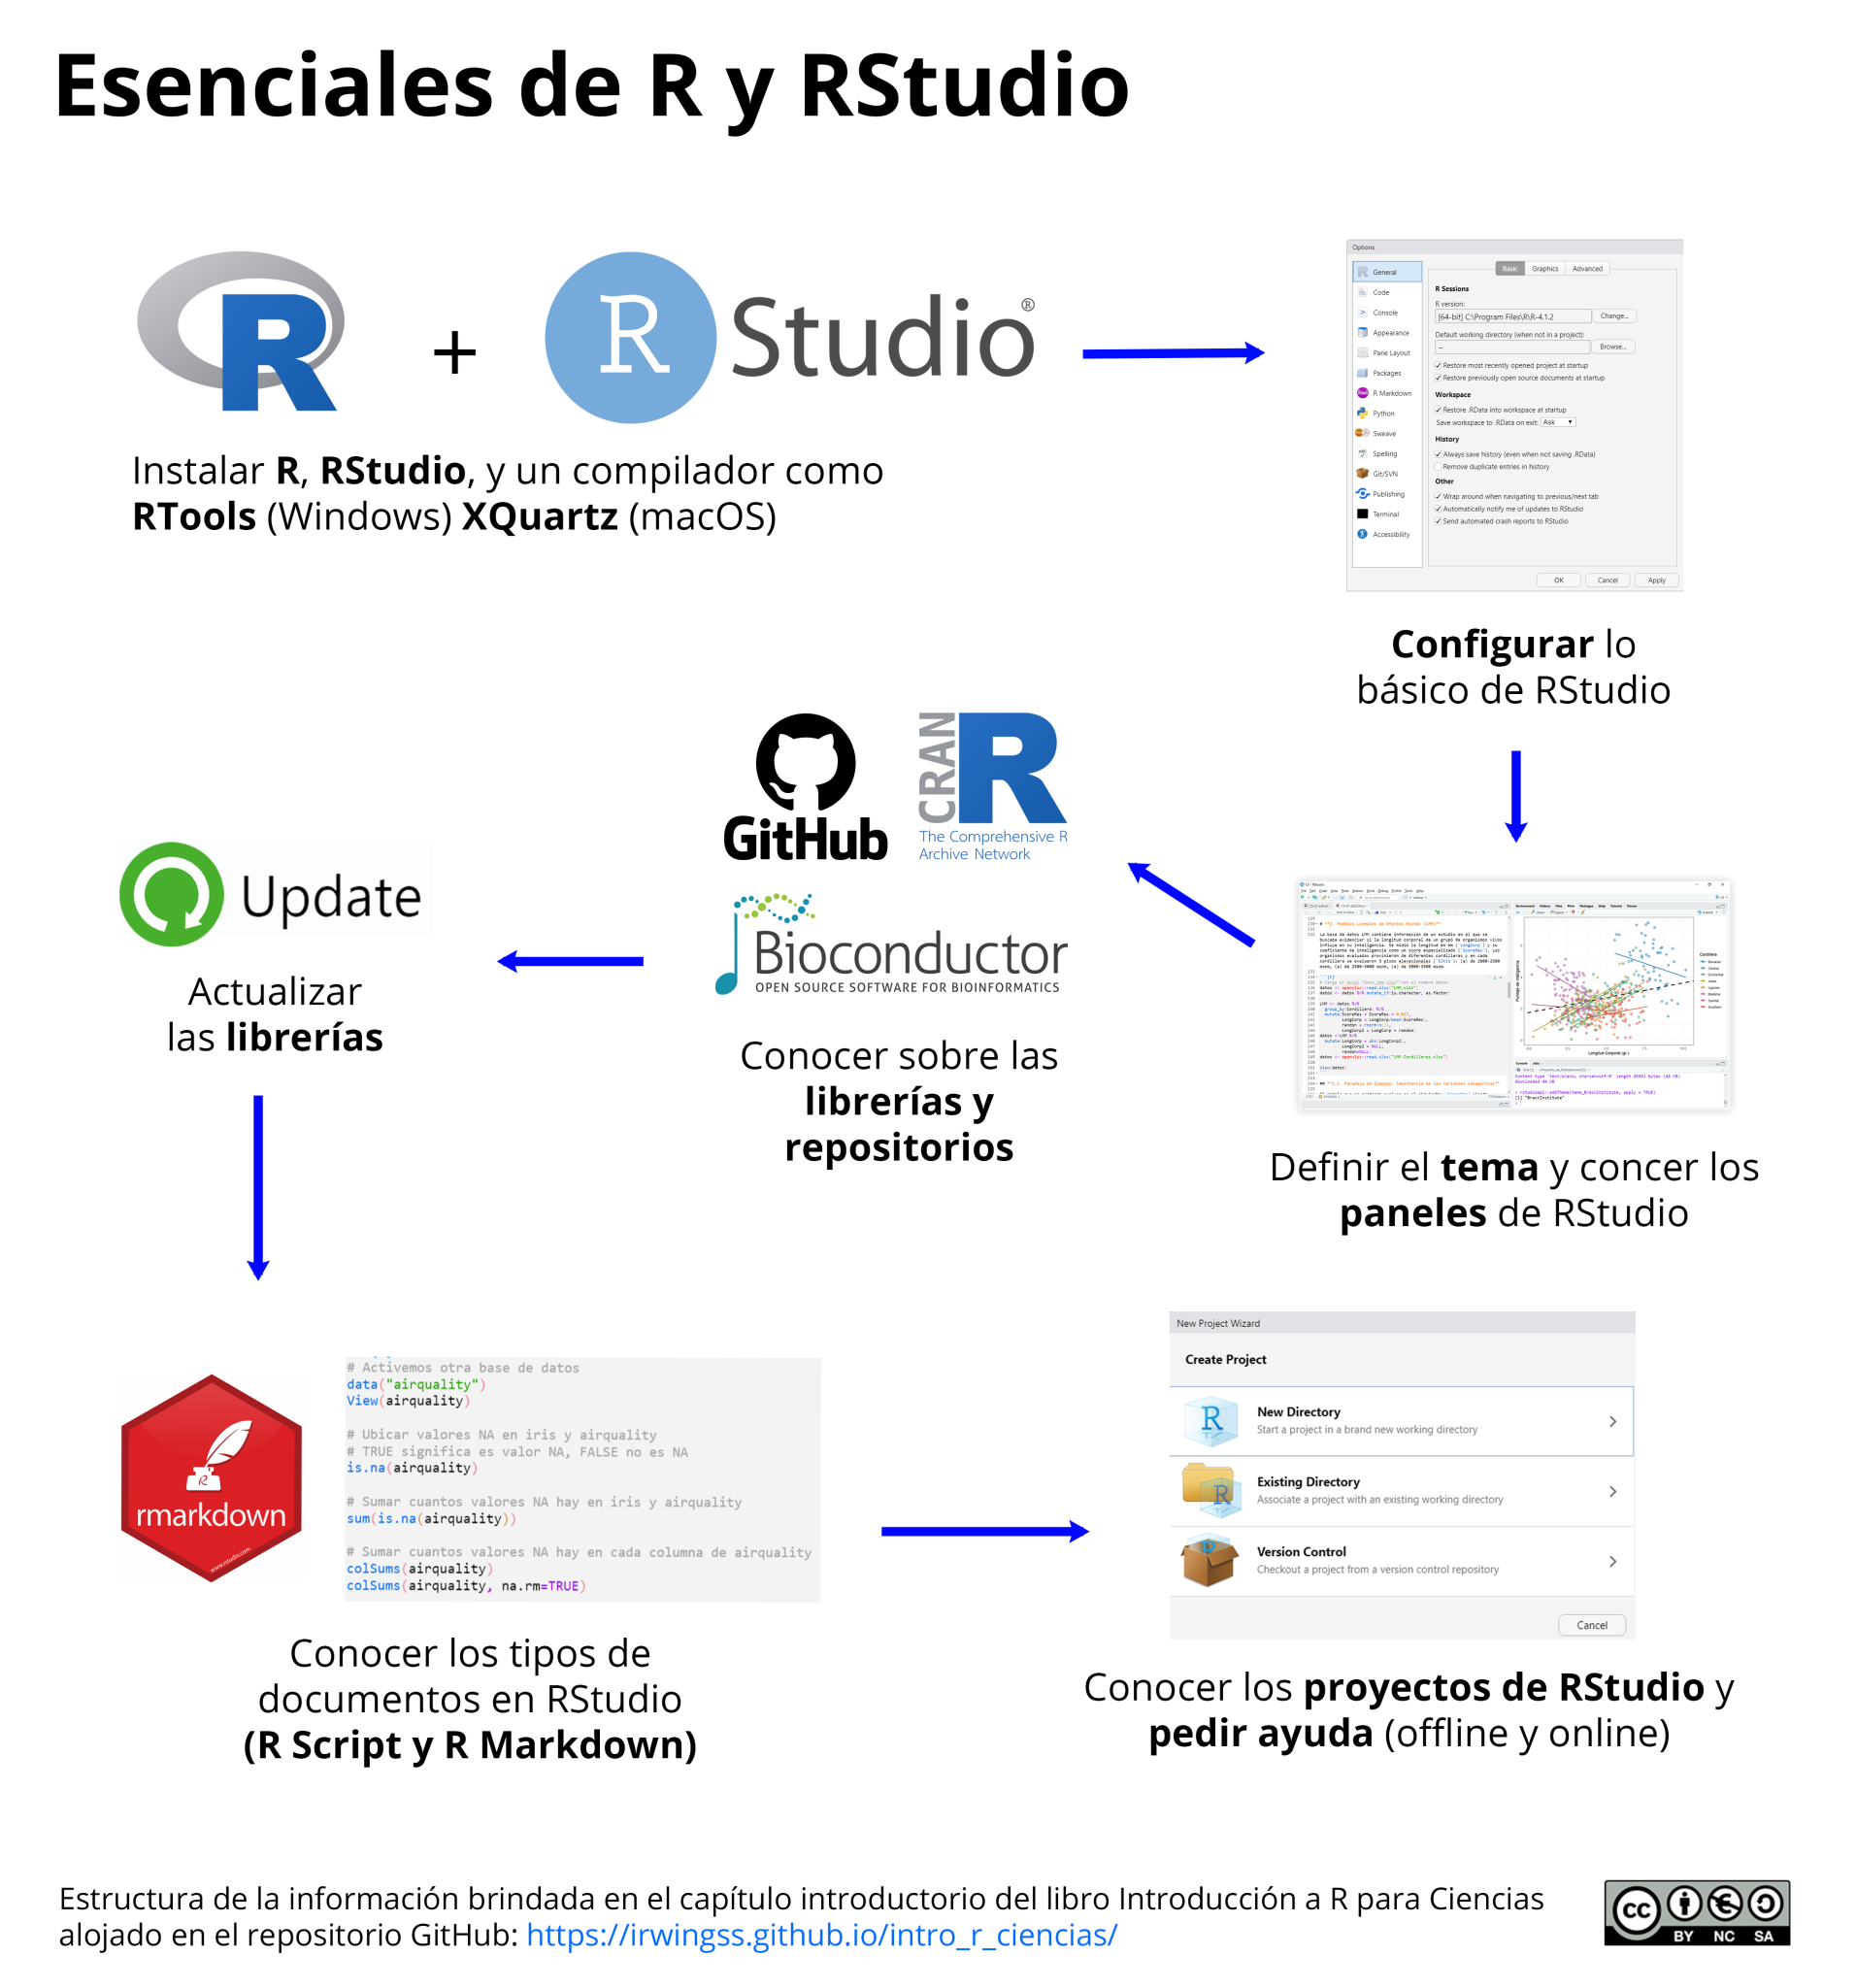
\includegraphics[width=1\linewidth]{figs/elaboradas/Esenciales de RStudio} 

}

\caption{Estructura temática del capítulo ``Esenciales de R y RStudio''.}\label{fig:figura1}
\end{figure}

\hypertarget{instalaciuxf3n-de-r-y-rstudio}{%
\subsection{Instalación de R y RStudio}\label{instalaciuxf3n-de-r-y-rstudio}}

Para utilizar el lenguaje de programación R (en adelante R), proponemos el uso del ambiente de desarrollo integrado \href{https://www.rstudio.com/}{RStudio}. Este programa mejorará enormemente el flujo, la velocidad y la eficiencia de trabajo con R. RStudio es más que un editor de texto que resalta la sintaxis del código de R, sino que también permite tener paneles de trabajo organizados que facilitan su uso.

\begin{rmdwarning }
\textbf{Requerimientos mínimos del sistema para ejecutar RStudio:}

\begin{itemize}
\tightlist
\item
  Sistema con CPU de 64 bits. Con 32 bits es posible instalar R pero no las versiones más recientes de RStudio.
\item
  Procesadores de 2 núcleos (equivalente a Intel® Core™ i3 o AMD Ryzen™ 3).
\item
  4 Gb RAM.
\item
  Espacio en almacenamiento de 100 Gb.
\end{itemize}

\textbf{Requerimientos recomendados del sistema para ejecutar RStudio:}

\begin{itemize}
\tightlist
\item
  Procesadores de 4 a más núcleos (equivalente a Intel® Core™ i5 a más o AMD Ryzen™ 5 a más).
\item
  8 a más Gb RAM.
\item
  Más de 100 Gb de espacio de almacenamiento.
  \end{rmdwarning }
\end{itemize}

Para efectos de este libro, se deberá utilizar \textbf{las versiones listadas (o posteriores)} de los siguientes programas, según el sistema operativo:

\hypertarget{para-windows}{%
\paragraph*{Para Windows:}\label{para-windows}}
\addcontentsline{toc}{paragraph}{Para Windows:}

\begin{itemize}
\tightlist
\item
  R version 4.1.3 (2022-03-10) -- ``One Push-Up'' \href{https://cran.r-project.org/bin/windows/base/R-4.1.3-win.exe}{Descarga}
\item
  RStudio Desktop 2022.02.0+443 \href{https://download1.rstudio.org/desktop/windows/RStudio-2022.02.0-443.exe}{Descarga}
\item
  Rtools4.0 \href{https://cran.r-project.org/bin/windows/Rtools/rtools40v2-x86_64.exe}{Descarga}
\end{itemize}

\hypertarget{para-macos}{%
\paragraph*{Para macOS:}\label{para-macos}}
\addcontentsline{toc}{paragraph}{Para macOS:}

\begin{itemize}
\tightlist
\item
  R version 4.1.3 (2022-03-10) -- ``One Push-Up'' \href{https://cran.r-project.org/bin/macosx/base/R-4.1.3.pkg}{Descarga}
\item
  RStudio Desktop 2021.09.1+372 \href{https://download1.rstudio.org/desktop/macos/RStudio-2022.02.0-443.dmg}{Descarga}
\item
  XQuartz 2.8.1. \href{https://github.com/XQuartz/XQuartz/releases/download/XQuartz-2.8.1/XQuartz-2.8.1.dmg}{Descarga}
\end{itemize}

\hypertarget{para-ubuntudebian}{%
\paragraph*{Para Ubuntu/Debian:}\label{para-ubuntudebian}}
\addcontentsline{toc}{paragraph}{Para Ubuntu/Debian:}

A lo largo del libro no brindamos comentarios o soporte para el uso de R o RStudio en UNIX/GNU/Linux/Ubuntu. Las principales razones son que la mayoría de usuarios que aprenden R no suelen utilizar sistemas operativos de código libre, además de que algunos paquetes han presentado problemas al ser instalados.

Primero, se debe preparar el índice de paquetes del sistema:

\begin{verbatim}
sudo apt update
\end{verbatim}

\begin{verbatim}
sudo apt -y upgrade
\end{verbatim}

Luego, ejecuta:

\begin{verbatim}
sudo apt -y install r-base
\end{verbatim}

Con lo anterior ya se tiene R instalado. Más adelante, cuando se desee actualizar R, ejecuta el código:

\begin{verbatim}
sudo apt-get remove --purge r-base*
\end{verbatim}

Luego, añadir el repositorio de CRAN:

\begin{verbatim}
sudo gedit /etc/apt/source.list
\end{verbatim}

Para Instalar RStudio para Ubuntu 18, Ubuntu 20 o Debian 10

\begin{verbatim}
sudo apt-get install gdebi-core
wget https://download1.rstudio.org/desktop/bionic/amd64/rstudio-2022.02.0-443-amd64.deb
sudo gdebi rstudio-server-2021.09.2-382-amd64.deb
\end{verbatim}

Los pasos aquí detallados están publicados en la \href{https://www.rstudio.com/products/rstudio/download-server/debian-ubuntu/}{web oficial de RStudio}. Otros códigos interesantes puedes hallarlos en diferentes referencias como las del \href{http://www.upm.es/sfs/Rectorado/Gabinete\%20del\%20Rector/Notas\%20de\%20Prensa/2015/05/documentos/Instrucciones\%20de\%20instalaci\%C3\%B3n\%20de\%20R\%20y\%20RStudio.pdf}{Center for Open Middleware}.

\hypertarget{configuraciuxf3n-de-rstudio}{%
\subsection{Configuración de RStudio}\label{configuraciuxf3n-de-rstudio}}

La siguiente es una configuración sugerida para que RStudio sea visualizado de igual manera por todos los estudiantes que usen este libro, y se guíen mejor con la sintaxis del código, ordenamiento de paneles, codificación, idioma del texto, entre otros.



\begin{figure}

{\centering \includegraphics[width=1\linewidth]{figs/screenshots/configRStudio-1} 

}

\caption{Para iniciar la configuración de RStudio, clic en \texttt{tools/\ Global\ Options}.}\label{fig:figura2}
\end{figure}



\begin{figure}

{\centering \includegraphics[width=1\linewidth]{figs/screenshots/configRStudio-2} 

}

\caption{Abrirá la ventana de configuraciones. En la pestaña General se verifica la versión de R que está ejecutando RStudio.}\label{fig:figura3}
\end{figure}



\begin{figure}

{\centering \includegraphics[width=1\linewidth]{figs/screenshots/configRStudio-3} 

}

\caption{En la pestaña Code se configura la mayor cantidad de puntos necesarios para que el código sea legible. Aquí se muestra la configuración de las pestañas Editing y Display. Las dos opciones nuevas en la versión de RStudio 1.4+ son (con flechas rojas), son importantes en mejorar la lectura del código para principiantes: una permite identificar los pares de paréntesis con colores diferenciables (Rainbow parentheses en pestaña Display), y la otra es un primer intento de crear un operador pipe nativo para el código básico de R (Use native pipe operator, \texttt{\textbar{}\textgreater{}}). Este último no lo habilitaremos para seguir usando el pipe de tidyverse \texttt{\%\textgreater{}\%}.}\label{fig:figura4}
\end{figure}



\begin{figure}

{\centering \includegraphics[width=1\linewidth]{figs/screenshots/configRStudio-4} 

}

\caption{En la pestaña Saving es importante definir la codificación que usarán los archivos generados por RStudio. Se recomienda dar clic en \texttt{Change...} y luego seleccionar la codificación \texttt{UTF-8}.}\label{fig:figura5}
\end{figure}



\begin{figure}

{\centering \includegraphics[width=1\linewidth]{figs/screenshots/configRStudio-6} 

}

\caption{Las pestañas Completion y Diagnóstico no se modifican mucho, pero sí es necesario mencionar que si notáse que el programa se ejecuta muy lento, se debe considerar desactivar las opciones de diagnóstico (marcadas en rojo).}\label{fig:figura6}
\end{figure}



\begin{figure}

{\centering \includegraphics[width=1\linewidth]{figs/screenshots/configRStudio-7} 

}

\caption{La organización de los paneles descritos en la sección \protect\hyperlink{panelesRStudio}{1.4 Paneles de RStudio} se configuran previamente en la pestaña Pane Layout. A la izquierda: la organización por defecto. A la derecha: se deberá seleccionar todas las pestañas (excepto VCS y Connections) con un check dentro del panel superior derecho. Eso hará que el panel inferior derecho cambie de nombre a ``TabSet''.}\label{fig:figura7}
\end{figure}



\begin{figure}

{\centering \includegraphics[width=1\linewidth]{figs/screenshots/configRStudio-8} 

}

\caption{El siguiente paso es cambiar la ubicación de TabSet haciendo clic y cambiando el panel por Console. Clic en Aplicar para definir los cambios.}\label{fig:figura8}
\end{figure}



\begin{figure}

{\centering \includegraphics[width=1\linewidth]{figs/screenshots/configRStudio-9} 

}

\caption{La configuración de R Markdown es solo para evitar que se cuelgue al usar los documentos. Definir todas las casillas y selectores como se muestra a continuación en las pestañas Basic y Advanced.}\label{fig:figura9}
\end{figure}



\begin{figure}

{\centering \includegraphics[width=1\linewidth]{figs/screenshots/configRStudio-10} 

}

\caption{Para trabajar correctamente con los documentos R Markdown y evitar que se cuelguen, desmarcar la casilla con flecha roja. En la pestaña Spelling, se especifica el uso del lenguaje para el texto de los documentos. Selecciona de la lista ``Spanish''. Clic en Aplicar para definir los cambios.}\label{fig:figura10}
\end{figure}

\hypertarget{nuevas-caracteruxedsticas-de-rstudio-versiuxf3n-2022-actualizado-23-02-22}{%
\subsection{Nuevas características de RStudio versión 2022 (Actualizado: 23-02-22)}\label{nuevas-caracteruxedsticas-de-rstudio-versiuxf3n-2022-actualizado-23-02-22}}

Durante febrero de 2022 se actualizó RStudio a la primera versión del año: 2022.02.0+443. En esta versión, el soporte gráfico fue actualizado, además de permitir algunos cambios en la visualización de R Markdown. El detalle de la actualización publicada por Studio Blog está \href{https://www.rstudio.com/blog/rstudio-2022-02-0-what-s-new/}{disponible aquí}.



\begin{figure}

{\centering \includegraphics[width=1\linewidth]{figs/screenshots/actualizacion RStudio 2022} 

}

\caption{En la sección de R Markdown, pestaña Visual, apareció una nueva opción para numerar las líneas de código dentro de cada code chunk (flecha roja izquierda, cambio visualizado en la flecha roja derecha). Además, la forma de cambiar del modo editor visual (Visual) a editor de código (Source) está dispuesto de manera más elegante. Estos cambios, están acompañados en mejoras en la salida gráfica y corrección de algunos problemas menores de los R Markdown.}\label{fig:figura11}
\end{figure}

\hypertarget{tema-brackinstitute-2022}{%
\subsection{Tema BrackInstitute (2022)}\label{tema-brackinstitute-2022}}

Este es un requerimiento especial para los estudiantes que usen este libro en las clases, en vivo o grabadas, del \href{https://www.brackinstitute.com/}{Instituto de Ciencias Antonio Brack} a través de la plataforma educativa online \href{https://www.masterx.org/}{masterX}. Se les solicita instalen el tema de color de RStudio \texttt{BrackInstitute} para que la sintaxis del código sea del mismo color que el mostrado en clase, facilitando así su comprensión. Si eres un lector que no está llevando el programa, sientete libre instalar el tema también.



\begin{figure}

{\centering \includegraphics[width=1\linewidth]{figs/screenshots/tema BrackInstitute} 

}

\caption{Vista previa del tema \texttt{BrackInstitute}.}\label{fig:figura12}
\end{figure}

Para instalarlo, copia las líneas de código completas en la consola.

\begin{Shaded}
\begin{Highlighting}[]
\FunctionTok{install.packages}\NormalTok{(}\StringTok{"xml2"}\NormalTok{)}
\FunctionTok{install.packages}\NormalTok{(}\StringTok{"rstudioapi"}\NormalTok{)}
\FunctionTok{install.packages}\NormalTok{(}\StringTok{"fs"}\NormalTok{)}
\NormalTok{tema\_BrackInstitute }\OtherTok{\textless{}{-}}\NormalTok{ fs}\SpecialCharTok{::}\FunctionTok{path\_temp}\NormalTok{(}\StringTok{"tema\_BrackInstitute"}\NormalTok{, }\AttributeTok{ext =} \StringTok{"tmTheme"}\NormalTok{)}
\FunctionTok{download.file}\NormalTok{(}\StringTok{"https://raw.githubusercontent.com/irwingss/Primolius{-}Theme/main/BrackInstitute.tmTheme"}\NormalTok{,tema\_BrackInstitute)}
\NormalTok{rstudioapi}\SpecialCharTok{::}\FunctionTok{addTheme}\NormalTok{(tema\_BrackInstitute, }\AttributeTok{apply =} \ConstantTok{TRUE}\NormalTok{)}
\end{Highlighting}
\end{Shaded}

Como se muestra a continuación:



\begin{figure}

{\centering \includegraphics[width=1\linewidth]{figs/screenshots/tema en consola} 

}

\caption{Código de instalación del tema \texttt{BrackInstitute} en la consola, listo para ser ejecutado.}\label{fig:figura13}
\end{figure}

Finalmente, presiona \texttt{enter} para comenzar su ejecución.

Si todo va bien, el tema cambiará automáticamente. Para más temas desarrollados para el Instituto de Ciencias Antonio Brack, visita el repositorio \href{https://github.com/irwingss/Primolius-Theme}{Primolius-Theme} de \href{https://github.com/irwingss}{Irwing S. Saldaña}.

\hypertarget{panelesRStudio}{%
\subsection{Paneles de RStudio}\label{panelesRStudio}}

Existen diversos editores de código que permiten trabajar con R, pero ninguno con la versatilidad de RStudio. El programa está dividido en paneles que uno puede reorganizar a conveniencia. Más allá de la posición o el orden de los paneles, es necesario que se sepa reconocerlos por su contenido, las pestañas que contiene, entre otros. Aquí se presentan los paneles en su posición clásica, junto con algunas barras y botones que se deben conocer al iniciar con RStudio.



\begin{figure}

{\centering \includegraphics[width=1\linewidth]{figs/screenshots/Slide1} 

}

\caption{Panel de Trabajo. Aquí aparecerán los archivos de trabajo de R, sean R script o R Markdown. Además, es donde aparecen las bases de datos cuando se pide visualizarlas en RStudio.}\label{fig:figura14}
\end{figure}



\begin{figure}

{\centering \includegraphics[width=1\linewidth]{figs/screenshots/Slide2} 

}

\caption{Consola. Es el panel donde se imprimen los resultados textuales y numéricos junto con el código que los genera.}\label{fig:figura15}
\end{figure}



\begin{figure}

{\centering \includegraphics[width=1\linewidth]{figs/screenshots/Slide3} 

}

\caption{Panel de pestañas: aquí encontrarás: el ambiente (Environment) donde se guardan los objetos creados o cargados en RStudio; la historia (History) de las ejecuciones realizadas durante la sesión de RStudio; archivos (Files) para visualizar los archivos de la carpeta de trabajo actual (definida como la carpeta ``documentos'' por defecto); la pestaña de visualización de gráficos estáticos (Plots); pestaña de instalación y actualización de paquetes (Packages); la pestaña de ayuda (Help); y el visualizador (Viewer) de gráficos animados, gráficos 3D, objetos HTML. las conexiones (Connections) que se pueden realizar con bases de datos (Oracle, SQL, Salesforce, Spark, Hipe, entre otros); tutoriales (tutorial) precargados usando shiny para el uso básico de R y RStudio.}\label{fig:figura16}
\end{figure}



\begin{figure}

{\centering \includegraphics[width=1\linewidth]{figs/screenshots/Slide6} 

}

\caption{Barra de opciones rápidas.}\label{fig:figura17}
\end{figure}



\begin{figure}

{\centering \includegraphics[width=1\linewidth]{figs/screenshots/Slide5} 

}

\caption{Barra de menús. De las pestañas más importantes: File nos permite crear o cargar archivos; Session, definir espacio de trabajo actual; y Tools, ingresar a las configuraciones de RStudio. Usos más avanzados, como la depuración de código o el uso de versiones de control (Git), también se manejan desde las opciones de esta barra.}\label{fig:figura18}
\end{figure}

\hypertarget{libreruxedas-y-repositorios}{%
\subsection{Librerías y Repositorios}\label{libreruxedas-y-repositorios}}

Una de las mayores virtudes de R es la enorme comunidad de desarrollo que ha creado asombrosas funcionalidades para simplificarle el flujo de trabajo a otras personas. Estas funcionalidades en realidad son \emph{funciones} (para mayor detalle sobre ellas, visita la sección \protect\hyperlink{funciones}{2.7 Funciones}). La estructura que almacena funciones se conoce como librería o paquete. Para poder una función en RStudio, se debe instalar previamente el paquete que la contiene. Los paquetes están publicados en repositorios. Los principales son:

\begin{itemize}
\item
  \href{https://cran.r-project.org/}{CRAN} (de Comprehensive R Archive Network en inglés), el repositorio oficial de R. Solo los paquetes aprobados y con soporte de fallos constante son publicados aquí.
\item
  \href{https://github.com/}{GitHub}, el repositorio más grande no oficial en el que se pueden encontrar paquetes de R. Muchos repositorios en CRAN mantienen versiones beta en GitHub para su testeo.
\item
  \href{https://www.bioconductor.org/}{Bioconductor}, el mayor repositorio de paquetes asociados a bioinformática y ciencias afines.
\end{itemize}



\begin{figure}

{\centering \includegraphics[width=1\linewidth]{figs/screenshots/paquetes instalacion} 

}

\caption{Instalación manual de paquetes.}\label{fig:figura19}
\end{figure}

Si se requiere instalar paquetes de CRAN (e.g., \textbf{tidyverse}) con código, se utilizará un código similar a este:

\begin{Shaded}
\begin{Highlighting}[]
\FunctionTok{install.packages}\NormalTok{(}\StringTok{"tidyverse"}\NormalTok{)}
\end{Highlighting}
\end{Shaded}

\hypertarget{actualizaciuxf3n-de-libreruxedas}{%
\subsection{Actualización de librerías}\label{actualizaciuxf3n-de-libreruxedas}}

Es importante mantener actualizada la paquetería. En los repositorios de cada paquete se suelen reportar fallos o inconsistencias que son resueltas y liberadas como una actualización. Se recomienda hacer esto al menos una vez por mes.



\begin{figure}

{\centering \includegraphics[width=1\linewidth]{figs/screenshots/paquetes actualizacion} 

}

\caption{Actualización manual de paquetes de CRAN.}\label{fig:figura20}
\end{figure}

Los paquetes instalados desde repositorio no oficial, deberán ser actualizados ``reinstalándolos'' de manera forzada. Para forzar la instalación de un paquete ya instalado desde github, se usa el argumento \texttt{force=TRUE}:

\begin{Shaded}
\begin{Highlighting}[]
\FunctionTok{install.packages}\NormalTok{(}\StringTok{"devtools"}\NormalTok{)}
\NormalTok{devtools}\SpecialCharTok{::}\FunctionTok{install\_github}\NormalTok{(}\StringTok{"irwingss/rbrack"}\NormalTok{, }\AttributeTok{force=}\ConstantTok{TRUE}\NormalTok{)}
\end{Highlighting}
\end{Shaded}

\begin{rmdnote}
Una vez instalados, los paquetes se almacenan en un estado no activo. Para usar sus funciones, se requiere \textbf{activar el paquete} que la contiene.
\end{rmdnote}

Para activar un paquete utiliza la función \texttt{library()}:

\begin{Shaded}
\begin{Highlighting}[]
\FunctionTok{library}\NormalTok{(tidyverse)}
\end{Highlighting}
\end{Shaded}

Desde el momento que se ejecuta el código anterior, \textbf{tidyverse} estará activo hasta que se cierre o reinicie el programa RStudio.

\begin{rmdnote}
Otra manera de usar una función es activar su uso puntualmente, sin activar toda la librería. En este respecto, el operador \texttt{::} permite acceder a las funciones de un paquete para seleccionar una y activar su uso
\end{rmdnote}

Para acceder puntualmente a la función \texttt{bind\_cols()} de la librería \textbf{dplyr}, se usa:

\begin{Shaded}
\begin{Highlighting}[]
\NormalTok{dplyr}\SpecialCharTok{::}\FunctionTok{bind\_cols}\NormalTok{()}
\end{Highlighting}
\end{Shaded}

\hypertarget{tipos-de-documentos-en-rstudio}{%
\subsection{Tipos de documentos en RStudio}\label{tipos-de-documentos-en-rstudio}}

Luego de conocer los paneles de RStudio, es necesario crear los espacios donde se escribirán las órdenes a modo de código. Estos documentos, como cualquier editor de texto, se pueden guardar o compartir, por ejemplo, mediante un correo electrónico.

\hypertarget{r-script-.r}{%
\subsubsection{R Script (.R)}\label{r-script-.r}}

Es el documento más simple donde puedo escribir R. Es un editor de texto como el bloc de notas de cualquier sistema operativo. No obstante, este editor lee y colorea la sintaxis especial del código de R. Esto permite identificar cada parte del código según lo que sea: una variable, una función, un número, un texto, símbolos especiales, operadores, entre otros; simplificando enormemente la lectura del código y el aprendizaje de R.

\begin{rmdnote}
Puedes crear un R script utilizando clics (ver Figura \ref{fig:figura21}), o con atajo de teclado: \texttt{Control\ +\ shift\ +\ N} (Windows) o \texttt{Command\ +\ shift\ +\ N} (MacOS).
\end{rmdnote}



\begin{figure}

{\centering \includegraphics[width=1\linewidth]{figs/screenshots/abrir un Rscript} 

}

\caption{Procedimiento para abrir un documento de RScript usando el menú \texttt{File/\ New\ File/\ R\ script}.}\label{fig:figura21}
\end{figure}



\begin{figure}

{\centering \includegraphics[width=1\linewidth]{figs/screenshots/Rscript} 

}

\caption{Apariencia de un R script con código. Notar los colores diferenciales para cada parte del código.}\label{fig:figura22}
\end{figure}

\hypertarget{r-markdown-.rmd}{%
\subsubsection{R Markdown (.Rmd)}\label{r-markdown-.rmd}}

Es un formato de archivo para la creación de documentos dinámicos. Estos pueden ser: páginas web, aplicaciones \textbf{shiny}, diapositivas, o cualquier tipo de reporte que puede ser exportado en formato .docx, .pdf o .html. Utiliza la sintaxis de Markdown pero posibilitando la inclusión de ``pedacitos de código'', la traducción literal de code chunk. Los chunk se comportan como pequeños R scripts embebidos en el documento de texto plano escrito con sintaxis Markdown.

Suena extremadamente complejo el decir ``sintaxis Markdown'', pero no lo es. Una vez uno sabe utilizar R, aprender Markdown resulta sencillo. Puedes aprender a utilizar R Markdown con el libro en línea \href{https://bookdown.org/yihui/rmarkdown/}{R Markdown: The Definitive Guide} en su versión de 2018, o el más actualizado \href{https://bookdown.org/yihui/rmarkdown-cookbook/}{R Markdown Cookbook} de 2020. Ambos libros han sido escritos en colaboración de Yihui Xie, uno de las mentes brillantes de RStudio y a quien le debemos el uso de documentos dinámicos en RStudio.

No se profundizará en el uso de R Markdown, dado que no es el objetivo del programa, pero se utilizará frecuentemente durante las clases. Si eres un estudiante que no ha está llevando el programa, podrás siempre utilizar tanto R script como R Markdown para ejecutar tus códigos. Se recomienda fuertemente comenzar a utilizar este último dada la ventaja de permitir hacer anotaciones de texto plano como en cualquier editor de texto común.



\begin{figure}

{\centering \includegraphics[width=1\linewidth]{figs/screenshots/abrir R Markdown 1} 

}

\caption{Procedimiento para abrir un documento de R Markdown usando el menú \texttt{File/\ New\ File/\ R\ Markdown...}.}\label{fig:figura23}
\end{figure}



\begin{figure}

{\centering \includegraphics[width=1\linewidth]{figs/screenshots/abrir R Markdown 2} 

}

\caption{Ventana emergente para darle nombre al documento R Markdown.}\label{fig:figura24}
\end{figure}



\begin{figure}

{\centering \includegraphics[width=1\linewidth]{figs/screenshots/abrir R Markdown 3} 

}

\caption{Aparecerá un archivo R Markdown con texto de ejemplo para que tengamos una idea de qué se puede hacer con él.}\label{fig:figura25}
\end{figure}



\begin{figure}

{\centering \includegraphics[width=1\linewidth]{figs/screenshots/abrir R Markdown 4} 

}

\caption{\texttt{knit} es una función del paquete \texttt{knitr}, desarrollado por Yihui Xie y colaboradores, para la generación de reportes dinámicos con R Markdown. Haciendo clic en el botón se despliega la lista de posibles exportaciones del documento. La exportación \texttt{Knit\ to\ HTML} produce una página web de reporte.}\label{fig:figura26}
\end{figure}



\begin{figure}

{\centering \includegraphics[width=1\linewidth]{figs/screenshots/abrir R Markdown 5} 

}

\caption{Tras hacer clic en \texttt{Knit\ to\ HTML}, será necesario guardar en el almacenamiento de la computadora el documento, cuya extensión es \texttt{.Rmd}.}\label{fig:figura27}
\end{figure}



\begin{figure}

{\centering \includegraphics[width=1\linewidth]{figs/screenshots/abrir R Markdown 6} 

}

\caption{En la consola, o en una pestaña Render, comenzará a mostrarse la ejecución del código que \texttt{knit} desplegó para exportar el R Markdown a página web HTML.}\label{fig:figura28}
\end{figure}



\begin{figure}

{\centering \includegraphics[width=1\linewidth]{figs/screenshots/abrir R Markdown 7} 

}

\caption{Vista del archivo HTML generado a partir del R Markdown de ejemplo.}\label{fig:figura29}
\end{figure}

\hypertarget{proyectos-de-rstudio}{%
\subsection{Proyectos de RStudio}\label{proyectos-de-rstudio}}

Este es el santo grial del uso de RStudio para crear una diversidad de repositorios: de trabajo, \href{https://medium.com/@jonathanmines/the-ultimate-github-collaboration-guide-df816e98fb67}{colaboraciones}, \href{https://bookdown.org/yihui/rmarkdown/xaringan.html}{diapositivas}, \href{https://rmarkdown.rstudio.com/lesson-13.html}{páginas web}, \href{https://bookdown.org/yihui/blogdown/}{blogs}, \href{https://bookdown.org/}{libros}, entre otros. Para poder usar un proyecto de RStudio con dichos propósitos, se necesita aprender a usar las versiones de control de proyectos con \href{https://happygitwithr.com/install-git.html}{Git} y \href{https://cfss.uchicago.edu/setup/shell/}{Shell}. Puedes iniciar en este tema con una genial presentación de su uso, elaborado por \href{https://www.geo.uzh.ch/microsite/reproducible_research/post/rr-rstudio-git/}{University of Zurich}.

Este apartado solo se centrará en el uso de proyectos para trabajos locales. Una vez se domine este uso, será más sencillo entender cómo elaborar otras cosas más complejas.

Aquí se muestran los pasos para crear un proyecto local:



\begin{figure}

{\centering \includegraphics[width=1\linewidth]{figs/screenshots/proyectos1} 

}

\caption{Para crear un proyecto local, ir a menu \texttt{File/\ New\ Project...}.}\label{fig:figura30}
\end{figure}



\begin{figure}

{\centering \includegraphics[width=1\linewidth]{figs/screenshots/proyectos2} 

}

\caption{Para efectos de este libro, selecciona la primera opción. Clic en \texttt{New\ Directory} para crear en el almacenamiento de tu computador una carpeta nueva donde se almacenará todo los respecto a este proyecto. \texttt{Existing\ Directory} solo se usará cuando ya se ha creado de antemano una carpeta donde se quiere almacenar el proyecto. Para versiones de control con Git y GitHub, el proceso se inicia con \texttt{Version\ Control}, para crear la carpeta de trabajo (tal como las anteriores opciones), pero el proyecto estará \emph{casi} listo para hacer \emph{commit} y publicar los cambios en GitHub.}\label{fig:figura31}
\end{figure}



\begin{figure}

{\centering \includegraphics[width=1\linewidth]{figs/screenshots/proyectos3} 

}

\caption{En \texttt{Directory\ name:} escribe el nombre del proyecto, mismo que también tendrá la nueva carpeta de trabajo que se creará en tu computador. En el botón \texttt{Browse...}, podrás ubicar una carpeta \emph{madre} donde irás creando proyectos para mantenerlos todos ordenados y accesibles. Puede ser una subcarpeta dentro de documentos, con algún nombre genérico como ``proyectos'', ``proyectos de R'', entre otros. Finalmente, clic en \texttt{Create\ Project}.}\label{fig:figura32}
\end{figure}



\begin{figure}

{\centering \includegraphics[width=1\linewidth]{figs/screenshots/proyectos4} 

}

\caption{Se abrirá una nueva sesión con título idéntico a la carpeta de proyecto creada (aquí ``Investigación A''). Nótese el ambiente (environment) en blanco. Todas las variables y funciones que se creen o carguen en el proyecto permanecerán en este ambiente específico del proyecto.}\label{fig:figura33}
\end{figure}



\begin{figure}

{\centering \includegraphics[width=1\linewidth]{figs/screenshots/proyectos5} 

}

\caption{En la pestaña de \texttt{Files} se verá el contenido de todo lo que copiemos dentro de la carpeta del proyecto. Puedes acceder a la carpeta de trabajo haciendo clic en \texttt{More/\ Show\ Folder\ in\ New\ Windows}. Allí podrás pegar archivos o documentos que necesites cargar posteriormente en tu proyecto.}\label{fig:figura34}
\end{figure}



\begin{figure}

{\centering \includegraphics[width=1\linewidth]{figs/screenshots/proyectos6} 

}

\caption{Para crear un nuevo proyecto, abrir uno existente o cerrar el proyecto actual (flecha roja), existe el menú de acceso rápido que tiene el mismo nombre que tu proyecto actual. Para ver la dirección de la carpeta de trabajo en consola, ejecuta la función \texttt{getwd()}.}\label{fig:figura35}
\end{figure}



\begin{figure}

{\centering \includegraphics[width=1\linewidth]{figs/screenshots/proyectos7} 

}

\caption{En tu computador, encontrarás creada la carpeta del proyecto, en la dirección que especificaste, donde podrás pegar los archivos que aparecerán en la pestaña de Files del Panel de Ambiente del proyecto.}\label{fig:figura36}
\end{figure}

\begin{rmdnote}
\begin{itemize}
\item
  Para ver la dirección de la carpeta de trabajo en consola, ejecuta la función \texttt{getwd()}.
\item
  Si necesitas cambiar manualmente tu proyecto a otro directorio (carpeta) de trabajo, ejecuta la función \texttt{setwd()} definiendo dentro de ella y entre comillas la nueva dirección deseada. Por ejemplo:

  \texttt{setwd("C:/Users/irwin/Documents/Otra\_Carpeta/Subcarpeta\ B")}
\item
  No olvides las comillas al inicio y final de la dirección, ni que los slash usados son forwardslash (hacia delante) \texttt{/}, no backslash (hacia atrás) \texttt{\textbackslash{}}.
  \end{rmdnote}
\end{itemize}

\hypertarget{pedir-ayuda}{%
\subsection{Pedir ayuda}\label{pedir-ayuda}}

Pedir ayuda sin internet es algo posible en RStudio. Todas las librerías instaladas contienen información de respaldo sobre el uso de cada función que almacenan.

Para acceder a ella, se debe acceder a la pestaña Help.



\begin{figure}

{\centering \includegraphics[width=1\linewidth]{figs/screenshots/help1} 

}

\caption{Accediendo a la pestaña Help para buscar ayuda sobre la función \texttt{mean()}. Nótese que solo se busca el nombre de la función sin paréntesis.}\label{fig:figura37}
\end{figure}



\begin{figure}

{\centering \includegraphics[width=1\linewidth]{figs/screenshots/help2} 

}

\caption{Detalle de la ayuda de la función \texttt{mean()}. Es muy útil revisar la sección Arguments donde se describen los argumentos, además los ejemplos de uso.}\label{fig:figura38}
\end{figure}

\begin{rmdnote}
\begin{itemize}
\item
  Es posible \textbf{pedir ayuda con código}. Ejecutando la función \texttt{help()} conteniendo el nombre de la \emph{función} que se desea buscar, abrirá automáticamente la página de ayuda en la pestaña Help. Por ejemplo:\texttt{help(varimax)}.
\item
  Otra forma de obtener el mismo resultado es usando el símbolo \texttt{?}. Por ejemplo: \texttt{?varimax}.
\item
  Si se necesita buscar un \emph{término}, no una función, se usaría el simbolo doble \texttt{??} antes del término a buscar. Esta búsqueda es más lenta porque es más profunda y nos da todas las funciones donde se use dicho término. Por ejemplo, para buscar en todos archivos de ayuda de R el término deviance: \texttt{??deviance}.
  \end{rmdnote}
\end{itemize}

Para pedir ayuda en internet, se recomienda el uso del buscador exclusivo de temas en R conocido como \href{https://rseek.org/}{rseek}.



\begin{figure}

{\centering \includegraphics[width=1\linewidth]{figs/screenshots/rseek} 

}

\caption{Búsqueda de ayuda para la función \texttt{mean()} en rseek. Puedes acceder directamente a la viñeta (PDF o web) del uso de la función (que es la misma información que en la búsqueda en RStudio), documentación, funciones asociadas, paquetes populares que usen mean, wikipedia, blogs como \href{https://www.r-bloggers.com/}{R-Bloggers} donde expliquen su uso, \emph{Issues} que son problemas reportados para la función, o paquetes que contengan una función con el mismo nombre.}\label{fig:figura39}
\end{figure}

\hypertarget{rbasico}{%
\section{\texorpdfstring{\textbf{Primer contacto con R}}{Primer contacto con R}}\label{rbasico}}

Este capítulo se centra en el manejo y comprensión del lenguaje de programación R (en adelante: ``R'') en nivel introductorio. Se asume que el lector tiene instalados y configurados los programas R, RStudio y algún otro programa de soporte para el manejo de paquetes. Si no cuentas con ninguno en tu computadora, visita el capítulo \protect\hyperlink{esencialesRRStudio}{1 Esenciales de R y RStudio}.

Una ventaja de los lenguajes de programación es que permiten al usuario definir una secuencia de órdenes (comandos) adaptadas a los requerimientos analíticos que tenga. El flujo de trabajo completo, el paso a paso, queda escrito en el código. Este puede ser compartido con colegas en trabajos colaborativos.

Antes de aprender sobre los métodos estadísticos de análisis que se revisarán en este libro, se necesita ``hablar'' correctamente el lenguaje R. Aprenderás a trabajar con el código básico en R, a crear variables para almacenar información, a crear funciones para agilizar el flujo de trabajo, a utilizar \texttt{tidyverse} para el manejo y limpieza de bases de datos, entre otros códigos útiles para inicar con R.

La forma simplificada de cómo funciona R se resume en escribir una orden, presionar ``algo'' para que la computadora comience a procesar la orden, y luego recibir un resultado textual o gráfico. Básicamente lo que hace cualquier otro lenguaje de programación.

No obstante, R es considerada una de los mejores lenguajes informáticos si nuestra orientación es más la investigación científica que el desarrollo informático. Otros lenguajes informáticos populares entre científicos son Python, MATLAB, C, C++, JavaScript, SQL, Scala, Julia, SAS, pero ninguno esta tan orientado al desarrollo estadístico como R.



\begin{figure}

{\centering \includegraphics[width=1\linewidth]{figs/screenshots/tema BrackInstitute} 

}

\caption{Ejemplo de uso de RStudio en el análisis estadístico.}\label{fig:figura40}
\end{figure}

R es considerada como una \emph{calculadora con esteroides} dado que puedes aplicar matemáticas con él; aquella ciencia sobre la que se cimentan casi todas las demás. Si puedes hacer ello, tienes las puertas abiertas a aplicar análisis estadísticos, generar gráficos y todo lo que te imagines. Y pues sí, también hay cosas algo bizarras en R, como poder crear tu propio \href{https://r-coder.com/calendarios-r/}{calendario} o usar \href{https://github.com/R-CoderDotCom/ggcats}{gatitos} en un gráfico de dispersión de puntos.

A diferencia de los lenguajes humanos (idiomas), un lenguaje de programación debe estar escrito a la perfección. No hay espacio para una coma mal puesta, un paréntesis olvidado, o un nombre errado. La computadora solo ejecutará la orden si todo está escrito exactamente, tal y como debe ser. Todos los ejemplos de este libro pueden ser ejecutados correctamente si se escriben como es mostrado, y si instalaste todo lo necesario para trabajar (revisa las secciones \protect\hyperlink{prerrequisitos}{Prerrequisitos} y \protect\hyperlink{esencialesRRStudio}{1 Esenciales de R y RStudio}.

\hypertarget{ejecutar-cuxf3digo}{%
\subsection{Ejecutar código}\label{ejecutar-cuxf3digo}}

¿Alguna vez hiciste un histograma de frecuencias?. Hacer uno de manera exploratoria es muy sencillo en R. El siguiente código hará dos cosas en un solo paso:

\begin{enumerate}
\def\labelenumi{\arabic{enumi}.}
\tightlist
\item
  Creará un conjunto de 10,000 datos aleatorios que siguen en la distribución normal.
\item
  Generará el gráfico del histograma de frecuencias utilizando el conjunto previamente creado.
\end{enumerate}

Por ahora no se ahondará en el detalle de qué cosa es \texttt{rnorm()} o \texttt{hist()}.

\begin{Shaded}
\begin{Highlighting}[]
\FunctionTok{hist}\NormalTok{(}\FunctionTok{rnorm}\NormalTok{(}\DecValTok{10000}\NormalTok{))}
\end{Highlighting}
\end{Shaded}

\begin{center}\includegraphics[width=1\linewidth]{02-primer-contacto_files/figure-latex/figura41-1} \end{center}

Para replicarlo, es necesario escribir el código exacto, para luego dar la orden, es decir, ejecutar el código. La ejecución se hace presionando en el teclado de tu computador \texttt{control\ +\ enter} o \texttt{command\ +\ enter} (usuarios macOS).

\begin{rmdnote}
Existen otros atajos de teclado para ejecuciones especiales.

\begin{itemize}
\tightlist
\item
  Ejecutar todas las líneas de código del script: \texttt{control\ (o\ command)\ +\ shift\ +\ enter}.
\item
  Ejecutar desde el inicio del script hasta la línea actual: \texttt{control\ (o\ command)\ +\ Alt\ +\ B}.
\item
  Ejecutar desde la línea actual hasta el final del script: \texttt{control\ (o\ command)\ +\ Alt\ +\ E}.
\end{itemize}

No obstante, no son necesarias. Es suficiente con conocer la ejecución básica, dado que para ejecutar varias líneas de código a la vez solo se deben seleccionar las requeridas y ejecutar con \texttt{control\ +\ enter} o \texttt{command\ +\ enter}.
\end{rmdnote}

Una pregunta que siempre genera confusión es la presencia de unos corchetes \texttt{{[}1{]}} en los resultados vistos tanto en consola como en este libro. Esto no es parte de un resultado por si mismo, es la posición del elemento mostrado justo a la derecha del corchete.

Si se ejecuta el símbolo \texttt{:} entre dos números, R generará el rango de valores enteros entre dichos números, incluyéndolos.

\begin{Shaded}
\begin{Highlighting}[]
\DecValTok{1}\SpecialCharTok{:}\DecValTok{100}
\CommentTok{\#   [1]   1   2   3   4   5   6   7   8   9  10  11  12  13  14  15  16  17  18  19}
\CommentTok{\#  [20]  20  21  22  23  24  25  26  27  28  29  30  31  32  33  34  35  36  37  38}
\CommentTok{\#  [39]  39  40  41  42  43  44  45  46  47  48  49  50  51  52  53  54  55  56  57}
\CommentTok{\#  [58]  58  59  60  61  62  63  64  65  66  67  68  69  70  71  72  73  74  75  76}
\CommentTok{\#  [77]  77  78  79  80  81  82  83  84  85  86  87  88  89  90  91  92  93  94  95}
\CommentTok{\#  [96]  96  97  98  99 100}
\end{Highlighting}
\end{Shaded}

El resultado muestra los confusos \texttt{{[}{]}} a la izquierda del primer elemento de cada fila del conjunto de datos resultante, indicando su posición dentro de la secuencia de elementos.

\hypertarget{r-como-calculadora}{%
\subsection{R como calculadora}\label{r-como-calculadora}}

Como ya se había mencionado antes, R nos permite operar con código. La cosa más sencilla para hacer en R es sumar.

\begin{Shaded}
\begin{Highlighting}[]
\DecValTok{10} \SpecialCharTok{+} \DecValTok{10}
\CommentTok{\# [1] 20}
\end{Highlighting}
\end{Shaded}

\begin{rstudio-tip}
En adelante se visualizará tanto el código a ejecutar (primera línea del ejemplo de suma aquí propuesto) como su resultado textual, mismo que obtendrás en la consola de RStudio (segunda línea del ejemplo) si sigues los pasos de cada ejemplo o ejercicio.
\end{rstudio-tip}

\begin{longtable}[]{@{}lllr@{}}
\caption{\label{tab:unnamed-chunk-5}Operaciones (símbolos) aritméticas en R}\tabularnewline
\toprule()
Operador & Operación & Ejemplo & Resultado \\
\midrule()
\endfirsthead
\toprule()
Operador & Operación & Ejemplo & Resultado \\
\midrule()
\endhead
\texttt{+} & Suma & \texttt{10\ +\ 3} & 13.000 \\
\texttt{-} & Resta & \texttt{10\ -\ \ 3} & 7.000 \\
\texttt{*} & Multiplicación & \texttt{10\ *\ 3} & 30.000 \\
\texttt{/} & División & \texttt{10\ /\ 3} & 3.333 \\
\texttt{\^{}} & Potencia & \texttt{10\ \^{}\ 3} & 1000.000 \\
\texttt{\%/\%} & División entera (parte entera) & \texttt{10\ \%\%\ 3} & 3.000 \\
\texttt{\%\%} & Residuo de dividir un número entre otro & \texttt{10\ \%/\%\ 3} & 1.000 \\
\bottomrule()
\end{longtable}

\hypertarget{funciones-matemuxe1ticas}{%
\subsubsection{Funciones matemáticas}\label{funciones-matemuxe1ticas}}

Operaciones más complejas necesitan el uso de funciones. Estas son ``secuencias de ordenes empaquetadas con un nombre pequeño y recordable'' --- la información sobre las funciones será desarrollada más adelante (\protect\hyperlink{funciones}{2.6 Funciones} y \protect\hyperlink{creacion-fun}{6.2 Creación de Funciones}). En la siguiente tabla se presentan las funciones matemáticas más comunes en R:

\begin{longtable}[]{@{}lllr@{}}
\caption{\label{tab:unnamed-chunk-6}Operaciones matemáticas en R. Estos procedimientos matemáticos vienen predefinidos como ordenes denominadas ``Funciones''.}\tabularnewline
\toprule()
Función & Operación & Ejemplo & Resultado \\
\midrule()
\endfirsthead
\toprule()
Función & Operación & Ejemplo & Resultado \\
\midrule()
\endhead
\texttt{exp(n)} & Eleva e a la n & \texttt{exp(3)} & 20.086 \\
\texttt{sqrt(n)} & Raíz cuadrada de n & \texttt{sqrt(3)} & 1.732 \\
\texttt{log(n)} & Logaritmo natural de n & \texttt{log(3)} & 1.099 \\
\texttt{log(n,\ b)} & Logaritmo de n en base b & \texttt{log(3,\ 10)} & 0.477 \\
\texttt{log10(n)} & Logaritmo de n en base 10 & \texttt{log10(3)} & 0.477 \\
\texttt{log1p(n)} & Logaritmo natural de n +1 & \texttt{log1p(2)} & 1.099 \\
\texttt{log2(n)} & Logaritmo en base 2 & \texttt{log2(10)} & 3.322 \\
\texttt{pi} & Número pi & \texttt{pi} & 3.142 \\
\texttt{abs(n)} & Convierte n en absoluto & \texttt{abs(-10.2)} & 10.200 \\
\bottomrule()
\end{longtable}

\hypertarget{operadores-luxf3gicos-y-relacionales}{%
\subsection{Operadores lógicos y relacionales}\label{operadores-luxf3gicos-y-relacionales}}

Además de poder operar matemáticamente dos objetos, los lenguajes de programación como R usan condiciones lógicas para definir estados de verdadero (\texttt{TRUE}) o falso (\texttt{FALSE}). Existen dos tipos de operadores en R para de definir un estado lógico:

Los operadores relacionales permiten comparar dos objetos y definir si la condición solicitada es verdadera o falsa. Por ejemplo: al preguntar a R si 10 es mayor que 9, definirá la condición lógica como verdadera. Este tipo de comparaciones pueden ser mayor, menor, mayor igual, menor igual, igual, no es igual o negación de un valor.

Los operadores lógicos permiten definir una condición lógica en base a los resultados de dos comparativas relacionales. Por ejemplo, si se desea filtrar las filas de una tabla para que se cumpla la \emph{condición 1}: valores mayores a 10 en la columna A \emph{y} la \emph{condición 2}: valores menores que 5 en la columna B, es preciso que ambas condiciones se cumplan para que una fila se muestre en el resultado final, gracias al operador \emph{y}. Si la condición usa el operador \emph{o}, tanto se cumpla una u otra condición, la fila se mostrará en el filtrado final.

En la siguiente tabla se muestran los operadores lógicos (últimos dos) y relacionales.

\begin{longtable}[]{@{}llll@{}}
\caption{\label{tab:unnamed-chunk-7}Operadores relacionales y lógicos en R, modos de uso y resultado lógico esperado (Verdadero o Falso).}\tabularnewline
\toprule()
Operador & Operación & Ejemplo & Resultado \\
\midrule()
\endfirsthead
\toprule()
Operador & Operación & Ejemplo & Resultado \\
\midrule()
\endhead
\texttt{!a} & \texttt{a} no es verdadero (negación de \texttt{a}) & \texttt{!TRUE} & FALSE \\
\texttt{==} & \texttt{a} es igual \texttt{b}, donde \texttt{b} es un solo elemento & \texttt{1\ ==\ 2} & FALSE \\
\texttt{\%in\%} & \texttt{a} es igual \texttt{b}, donde \texttt{b} es un conjunto de elementos & \texttt{1\ \%in\%\ c(2,3,1)} & TRUE \\
\texttt{!=} & \texttt{a} no es igual \texttt{b} & \texttt{A\ !=\ A} & FALSE \\
\texttt{\textgreater{}} & \texttt{a} es mayor que \texttt{b} & \texttt{10\ \textgreater{}\ 9} & TRUE \\
\texttt{\textless{}} & \texttt{a} es menor que \texttt{b} & \texttt{10\ \textless{}\ 9} & FALSE \\
\texttt{\textgreater{}=} & \texttt{a} es mayor igual que \texttt{b} & \texttt{10\ \textgreater{}=\ 9} & TRUE \\
\texttt{\textless{}=} & \texttt{a} es menor igual que \texttt{b} & \texttt{10\ \textless{}=\ 9} & FALSE \\
\texttt{\textbar{}} o \texttt{\textbar{}\textbar{}} & Se cumple la \texttt{Condición\ 1} o \texttt{Condición\ 2}. Si al menos una de las dos condiciones es verdadera, el resultado final es verdadero. & \texttt{9\ ==\ 10\ \textbar{}\ 10\ \textgreater{}\ 9} & TRUE \\
\texttt{\&} o \texttt{\&\&} & Se cumple la \texttt{Condición\ 1} y la \texttt{Condición\ 2}. Si ambas condiciones son verdadera, el resultado final es verdadero, de otro modo, falso. & \texttt{10\ ==\ 10\ \&\ 10\ \textgreater{}\ 9} & TRUE \\
\bottomrule()
\end{longtable}

\hypertarget{comentar-el-cuxf3digo}{%
\subsection{Comentar el código}\label{comentar-el-cuxf3digo}}

Una forma de asegurar que en el futuro el código escrito sea entendible, incluso por nosotros mismos, es comentándolo. Dejar comentarios nos ayudará a recordar la intención con la que se escribió una sección determinada de los comandos.

Para comentar en R, se requiere colocar el símbolo \texttt{\#} a la izquierda del texto a ser considerado comentario.

\begin{Shaded}
\begin{Highlighting}[]
\CommentTok{\# Esta es una suma }
\DecValTok{2} \SpecialCharTok{+} \DecValTok{2} 
\CommentTok{\# [1] 4}

\DecValTok{10} \SpecialCharTok{*} \DecValTok{2} \CommentTok{\# + 3029}
\CommentTok{\# [1] 20}
\end{Highlighting}
\end{Shaded}

Como queda en evidencia, no importa si el comentario está en solitario en una línea de código, o si está a la derecha de algo que sí se quiere ejecutar. Esto no afecta el resultado de la operación.

\hypertarget{creaciuxf3n-de-variables}{%
\subsection{Creación de variables}\label{creaciuxf3n-de-variables}}

Las variables son espacios virtuales, que puede contener de elementos o estar vacíos. Imagina que en una tabla de datos es un objeto ``contenedor de mediciones'' de un trabajo de investigación. Dicha tabla puede ser considerada una variable u objeto en R. Más adelante se hablará sobre los tipos de variables que existen en R.

Una forma sencilla de comenzar con variables es guardar un valor numérica en la memoria de trabajo de RStudio, también llamado ambiente (pestaña \emph{Environment}). En este sentido, se necesita \emph{asignar} el contenido a un nombre para que RStudio lo ``recuerde'', haciendo uso de un operador de asignación \texttt{\textless{}-}. Para crear una variable llamada NUM conteniendo el número 2022.

\begin{Shaded}
\begin{Highlighting}[]
\NormalTok{NUM }\OtherTok{\textless{}{-}} \DecValTok{2022}
\end{Highlighting}
\end{Shaded}

Si se desea ver el contenido de una variable previamente guardada en el ambiente, basta con ejecutar el nombre d ela variable:

\begin{Shaded}
\begin{Highlighting}[]
\NormalTok{NUM}
\CommentTok{\# [1] 2022}
\end{Highlighting}
\end{Shaded}

o usar la función \texttt{print()} para imprimirla en la consola:

\begin{Shaded}
\begin{Highlighting}[]
\FunctionTok{print}\NormalTok{(NUM)}
\CommentTok{\# [1] 2022}
\end{Highlighting}
\end{Shaded}

Una versión frecuentemente usada en ejemplos de R, involucra colocar a la asignación entre paréntesis para que hacer dos cosas a la vez: guardar la variable en el ambiente y mostrar su contenido en la consola.

\begin{Shaded}
\begin{Highlighting}[]
\NormalTok{(NUM }\OtherTok{\textless{}{-}} \DecValTok{2022}\NormalTok{)}
\CommentTok{\# [1] 2022}
\end{Highlighting}
\end{Shaded}

Existe la posibilidad de asignar con un operador de asignación inverso \texttt{-\textgreater{}}. Toma en cuenta qué debe ir en la cola (contenido) y en la cabeza (nombre) del operador. En otras palabras, la ``flecha'' que se forma con este operador siempre apunta al futuro nombre de la variable. Recuerda, la variable no existe hasta que no se ejecute y aparezca dicho nombre en el ambiente de RStudio.

\begin{Shaded}
\begin{Highlighting}[]
\CommentTok{\# Operador de asignación inverso}
\DecValTok{2022} \OtherTok{{-}\textgreater{}}\NormalTok{ NUM}
\end{Highlighting}
\end{Shaded}

El símbolo \texttt{=} también funciona, pero, por convención, este no se debe usar para crear variables. Se usará dentro de las funciones para ``asignar'' contenido a los argumentos de las mismas (se explicará a continuación).

\begin{Shaded}
\begin{Highlighting}[]
\CommentTok{\# Mal uso del símbolo =}
\NormalTok{NUM }\OtherTok{=} \DecValTok{2022}

\CommentTok{\# Buen uso del símbolo = : siempre dentro de una función.}
\CommentTok{\# Calcular el logaritmo en base 2 de 10}
\NormalTok{bs }\OtherTok{\textless{}{-}} \DecValTok{2} \SpecialCharTok{+} \DecValTok{8}
\FunctionTok{log}\NormalTok{(}\DecValTok{10}\NormalTok{, }\AttributeTok{base =}\NormalTok{ bs)}
\CommentTok{\# [1] 1}
\end{Highlighting}
\end{Shaded}

\begin{rstudio-tip}
Ciertamente, en el ejemplo anterior no fue esencial guardar la variable \texttt{bs} en el ambiente para su uso posterior dentro de \texttt{log()}. Sabemos de antemano que la suma es \texttt{10}. No obstante, este ejemplo nos da idea de como aplicar el guardar un resultado para usarlo luego en ejercicios más complejos.
\end{rstudio-tip}

No es posible continuar hablando de variables sin antes hacer una introducción a las funciones en R.

\hypertarget{funciones}{%
\subsection{Funciones}\label{funciones}}

Se puede idealizar una función como una secuencia de órdenes (líneas de código) que tienen como objetivo aplicarle un procedimiento (gráfico, estadístico, de modificación o transformación, entre otros) a un objeto de entrada (input) para generar un resultado (ouput). Dichas líneas de código están empaquetadas y almacenadas con un nombre.

Reconocer una función en R es tarea sencilla, siempre será un nombre seguido de paréntesis. Por ejemplo, la función para calcular la desviación estándar de un conjunto de datos es \texttt{sd()}, que proviene del inglés \emph{standard deviation}. Dentro de los paréntesis se deben colocar los argumentos de la función. El argumento más sencillo que algunas funciones necesitan es un conjunto de datos, y es justamente lo único que necesita \texttt{sd()}.

\begin{Shaded}
\begin{Highlighting}[]
\CommentTok{\# Para crear un conjunto de datos en R se usa la función c()}
\NormalTok{x }\OtherTok{\textless{}{-}} \FunctionTok{c}\NormalTok{(}\DecValTok{7}\NormalTok{,}\DecValTok{9}\NormalTok{,}\DecValTok{3}\NormalTok{,}\DecValTok{4}\NormalTok{,}\DecValTok{5}\NormalTok{,}\DecValTok{3}\NormalTok{,}\DecValTok{7}\NormalTok{,}\DecValTok{8}\NormalTok{)}

\CommentTok{\# Usando sd() para hallar la desviación estándar de x}
\FunctionTok{sd}\NormalTok{(x)}
\CommentTok{\# [1] 2.315}
\end{Highlighting}
\end{Shaded}

Si se ejecuta únicamente el nombre de una función existente en RStudio, en la consola se mostrará el contenido de la misma, la secuencia de órdenes que le dan forma a la función. Ejecuta el \texttt{sd} para ver su contenido:

\begin{Shaded}
\begin{Highlighting}[]
\NormalTok{sd}
\CommentTok{\# function (x, na.rm = FALSE) }
\CommentTok{\# sqrt(var(if (is.vector(x) || is.factor(x)) x else as.double(x), }
\CommentTok{\#     na.rm = na.rm))}
\CommentTok{\# \textless{}bytecode: 0x0000020985342ee0\textgreater{}}
\CommentTok{\# \textless{}environment: namespace:stats\textgreater{}}
\end{Highlighting}
\end{Shaded}

La secuencia de órdenes dentro de \texttt{sd} es corta. Básicamente utiliza la función \texttt{sqrt()} para sacarle la raíz cuadrada a la función \texttt{var()}, esta última calcula la varianza de un conjunto de datos. La estructura del código es propiamente la fórmula matemática para el cálculo de la desviación estándar. Aunque, a decir verdades, el código luce más complejo, y es debido a que aquí la función \texttt{var()} contiene argumentos condicionales para pedir que evalúe si el objeto \texttt{x} es correcto para la función, o si se necesita un cambio antes de procesar\texttt{x} en \texttt{sd()}. Pierde cuidado si no se entiende mucho por ahora, no es necesario comprender las funciones a este nivel al iniciar con R.

\hypertarget{funciones-buxe1sica-uxfatiles}{%
\subsection{Funciones básica útiles}\label{funciones-buxe1sica-uxfatiles}}

En gran medida, las primeras etapas del aprendizaje de R involucran \emph{entender}, siendo prioritario comprender qué dice un código y cómo se interpreta, más allá de escribirlo de memoria. En este sentido, la mayoría de funciones están nombradas de tal manera que indican para qué se pueden usar. Un dominio básico del idioma inglés será de mucha utilidad, principalmente porque casi todas las funciones de R están nombradas en inglés.

Para facilitar esta primera etapa de aprendizaje, aquí se muestra una lista de funciones básica útiles, tanto a nivel de programación como de análisis de datos, que serán clave para iniciar con R.

Los ejemplos de uso de la tabla son aplicables, siempre y cuando se ejecute antes el siguiente código para activar la base de datos \texttt{iris}, y crear los vectores \texttt{x}, \texttt{y}, y \texttt{letras}.

\begin{Shaded}
\begin{Highlighting}[]
\FunctionTok{data}\NormalTok{(}\StringTok{"iris"}\NormalTok{)}
\FunctionTok{set.seed}\NormalTok{(}\DecValTok{123}\NormalTok{)}
\NormalTok{x }\OtherTok{\textless{}{-}} \FunctionTok{rnorm}\NormalTok{(}\DecValTok{30}\NormalTok{,}\DecValTok{2}\NormalTok{,}\DecValTok{1}\NormalTok{)}
\NormalTok{y }\OtherTok{\textless{}{-}} \FunctionTok{rnorm}\NormalTok{(}\DecValTok{30}\NormalTok{,}\DecValTok{5}\NormalTok{,}\DecValTok{3}\NormalTok{)}\SpecialCharTok{*}\NormalTok{x}\SpecialCharTok{/}\DecValTok{2}
\NormalTok{letras }\OtherTok{\textless{}{-}} \FunctionTok{c}\NormalTok{(}\StringTok{"A"}\NormalTok{, }\StringTok{"B"}\NormalTok{, }\StringTok{"A"}\NormalTok{, }\StringTok{"A"}\NormalTok{)}
\end{Highlighting}
\end{Shaded}

\begin{longtable}[]{@{}lll@{}}
\caption{\label{tab:unnamed-chunk-19}Funciones básicas útiles en R.}\tabularnewline
\toprule()
Función & Descripción & Ejmplo.de.uso \\
\midrule()
\endfirsthead
\toprule()
Función & Descripción & Ejmplo.de.uso \\
\midrule()
\endhead
\texttt{\textbar{}\textgreater{}} & Operador pipe nativo. & \texttt{x\ \textbar{}\textgreater{}\ round(2)} \\
\texttt{\%\textgreater{}\%} & Operador pipe de tidyverse. & \texttt{x\ \%\textgreater{}\%\ round(2)} \\
\texttt{mean()} & Promedio de un conjunto de datos \texttt{x}. & \texttt{mean(x)} \\
\texttt{median()} & Mediana de un conjunto de datos \texttt{x}. & \texttt{median(x)} \\
\texttt{sd()} & Desviación estándar de un conjunto de datos \texttt{x}. & \texttt{sd(x)} \\
\texttt{var()} & Varianza de un conjunto de datos \texttt{x}. & \texttt{var(x)} \\
\texttt{quantile()} & Cálculo de cuantiles de un conjunto de datos \texttt{x}. & \texttt{quantile(x)} \\
\texttt{range()} & Valor mínimo y máximo de un conjunto de datos \texttt{x}. & \texttt{range(x)} \\
\texttt{seq\_along()} & Crea una secuencia de números enteros desde 1 hasta el valor de la longitud de elementos del vector. & \texttt{seq\_along(x)} \\
\texttt{sum()} & Suma de todos los elementos numéricos de un conjunto de datos \texttt{x}. & \texttt{sum(x)} \\
\texttt{max()} & Valor máximo de un conjunto de datos \texttt{x}. & \texttt{max(x)} \\
\texttt{min()} & Valor mínimo de un conjunto de datos \texttt{x}. & \texttt{min(x)} \\
\texttt{seq()} & Calcula una secuencia de números al ofrecerle un inicio, un final y cada cuántos valores. & \texttt{seq(0,\ 10,\ 2)} \\
\texttt{seq()} & Calcula una secuencia de números al ofrecerle un inicio, un final y cada la cantidad de valores que necesito de dicho rango. & \texttt{seq(0,\ 10,\ length=25)} \\
\texttt{rep()} & Repite un vector una cantidad de veces definida. & \texttt{rep("Perú",\ 15)} \\
\texttt{paste0()} & Concatena dos elementos de texto sin espacio entre ellos & \texttt{paste0("Séptima","Maravilla")} \\
\texttt{paste()} & Concatena dos elementos de texto con espacio entre ellos & \texttt{paste("Séptima","Maravilla")} \\
\texttt{sort()} & Reordena un vector de mayor a menor, o alfabéticamente. & \texttt{sort(c("C","Z","A"))} \\
\texttt{rev()} & Muestra un vector en orden reverso. & \texttt{rev(c("C","Z","A"))} \\
\texttt{unique()} & Muestra los valores únicos de un vector \texttt{x}. & \texttt{unique(letras)} \\
\texttt{scale()} & Estandariza (centrado y escalado) un conjunto de datos x. & \texttt{scale(x)} \\
\texttt{lm()} & Calcula un modelo lineal, siguiendo una fórmula predefinida. & \texttt{lm(Petal.Length\ \textasciitilde{}\ Sepal.Length,\ data=iris)} \\
\texttt{glm()} & Calcula un modelo generalizado lineal, siguiendo una fórmula predefinida. & \texttt{glm(Petal.Length\ \textasciitilde{}\ Sepal.Length,\ data=iris)} \\
\texttt{aov()} & Calcula un ANOVA, siguiendo una fórmula predefinida. & \texttt{aov(Petal.Length\ \textasciitilde{}\ Species,\ data=iris)} \\
\texttt{summary()} & Ofrece un resumen estadístico de un objeto especial, un vector o una base de datos. & \texttt{summary(x)} \\
\texttt{chisq.test()} & Prueba de Chi cuadrado de dos variables. & \texttt{chisq.test(x,\ y)} \\
\texttt{t.test()} & Prueba de T de dos variables. & \texttt{t.test(x,\ y)} \\
\texttt{cor.test()} & Correlación (\texttt{pearson}, \texttt{kendall}, \texttt{spearman}) de dos conjuntos de datos. & \texttt{cor.test(x,\ y,\ method="pearson")} \\
\texttt{plot()} & Realizá un gráfico de dispersión de puntos entre dos vectores numéricos. & \texttt{plot(x,\ y)} \\
\texttt{pairs()} & Genera un gráfico de enfrentamientos pareados entre todas las columnas de una base de datos. & \texttt{pairs(DF)} \\
\texttt{hist()} & Grafica un histograma de frecuencias de un vector \texttt{x}. & \texttt{hist(x)} \\
\texttt{boxplot()} & Grafica un gráfico de cajas de un vector \texttt{x}. & \texttt{boxplot(x)} \\
\texttt{plot(density())} & Produce el gráfico de función de densidad de un vector \texttt{x}. & \texttt{plot(density(x))} \\
\texttt{rnorm()} & Genera una cantidad de números aleatorios que siguen la distribución Normal, con parámetros definidos. & \texttt{rnorm(100,\ mean=1,\ sd=0)} \\
\texttt{set.seed()} & Especifíca que secuencia de números aleatorios usar. Permite replicabilidad de un evento aleatorio. & \texttt{set.seed(123)} \\
\texttt{getwd()} & Muestra la dirección del directorio de trabajo actual. & \texttt{getwd()} \\
\texttt{setwd()} & Define la nueva dirección del directorio de trabajo. & \texttt{setwd("C:/mi\ carpeta")} \\
\texttt{str()} & Muestra la estructura de una base de datos. & \texttt{str(iris)} \\
\texttt{View()} & Visualiza una base de datos en una nueva pestaña. & \texttt{View(iris)} \\
\texttt{names()} & Reporta los nombres de las columnas de una base de datos. & \texttt{names(iris)} \\
\texttt{colnames()} & Reporta los nombres de las columnas de una base de datos. & \texttt{colnames(iris)} \\
\texttt{rownames()} & Reporta los nombres de las filas de una base de datos. & \texttt{rownames(iris)} \\
\texttt{length()} & Reporta el número de elementos de un vector, o la cantidad de columnas de una base de datos. & \texttt{length(x)} o \texttt{length(iris)} \\
\texttt{nrow()} & Reporta la cantidad de filas de una base de datos. & \texttt{nrow(iris)} \\
\texttt{ncol()} & Reporta la cantidad de columnas de una base de datos. & \texttt{ncol(iris)} \\
\texttt{head()} & Muestra las primeras 6 filas de una data frame (DF) o tibble. & \texttt{head(DF)} \\
\texttt{tail()} & Muestra las últimas 6 filas de una data frame (DF) o tibble. & \texttt{tail(DF)} \\
\texttt{ls()} & Lista el nombre de todos los objetos en el ambiente. & \texttt{ls()} \\
\texttt{rm()} & Elimina una variable del ambiente de RStudio. & \texttt{rm(iris)} \\
\texttt{rm(ls())} & Elimina todas las variables del ambiente de RStudio. & \texttt{rm(ls())} \\
\texttt{dev.off()} & Cierra forzadamente la salida gráfica de RStudio. Ejecutar para cuando existe algún error en la generación de un gráfico. Además, permite terminar la exportación de un archivo gráfico. & \texttt{dev.off()} \\
\texttt{install.packages()} & Permite instalar una librería en RStudio. & \texttt{install.packages("tidyverse")} \\
\texttt{library()} & Permite activar durante la sesión actual una librería previamente instalada. & \texttt{library(tidyverse)} \\
\texttt{table()} & Muestra la frecuencia de los elementos únicos de un vector. & \texttt{table(letras)} \\
\texttt{subset()} & Devuelve un subgrupo de filas en una base de datos, filtradas si cumplen con una condición lógica. & \texttt{subset(iris,\ Petal.Length\ \textgreater{}\ 6.5)} \\
\texttt{sample()} & Devuelve un muestreo aleatorio de tamaño definido de un conjunto de datos x. & \texttt{sample(x,\ 3)} \\
\texttt{data()} & Permite cargar una base de datos de ejemplo preinstalada en RStudio dentro de algún paquete activo. & \texttt{data("iris")} \\
\texttt{round()} & Redondea un número a la cantidad de decimales establecida. & \texttt{round(0.00887,\ 2)} \\
\texttt{signif()} & Redondea un número a la cantidad de números significativos establecida. & \texttt{signif(0.00887,\ 2)} \\
\texttt{print()} & Imprime un objeto en la consola. Retorna el valor original.. & \texttt{print(x)} \\
\texttt{return()} & Imprime un objeto en la consola. Retorna el valor original.. & \texttt{return(x)} \\
\texttt{cut()} & Convierte a factor un vector, dividiéndolo (cortándolo) en la cantidad de grupos definidos. Clásica función para convertir un vector numérico de edades en rangos etarios. & \texttt{cut(1:20,\ breaks\ =\ 3)} \\
\texttt{cut()} & Los mismo que cut() pero dándole un nombre nuevo a cada nivel del factor. & \texttt{cut(1:20,\ breaks\ =\ 3)\ \textbar{}\textgreater{}\ factor(labels\ =\ c("A","B","C"))} \\
\texttt{print()} & Imprime un objeto en la consola. Retorna el valor original.. & \texttt{print(x)} \\
\texttt{return()} & Imprime un objeto en la consola. Retorna el valor original.. & \texttt{return(x)} \\
\bottomrule()
\end{longtable}

\hypertarget{ejercicios-del-capuxedtulo}{%
\subsection{Ejercicios del capítulo}\label{ejercicios-del-capuxedtulo}}

\begin{enumerate}
\def\labelenumi{\arabic{enumi}.}
\tightlist
\item
  Soluciona la ecuación \(\frac{24+12}{(2 * 3)^2}\).
\item
  Resuelve \(\mathrm{log_{10}}(|\frac{\mathrm{exp(10)}^2}{-10*9^{6}}|)\). Las barras verticales implican aplicar valor absoluto antes de calcular el logaritmo en base 10.
  1.La función sigmoidal \(\sigma(\mathrm{z}) = \frac{1}{1+e^{-\mathrm{z}}}\) es muy importante en estadística. Permite convertir el resultado de una regresión logística (Odds ratios) en probabilidades, facilitando la interpretación. Utiliza la fórmula \(z = -1.69 + 1*0.56\), emulando el resultado hipotético de una regresión logística, como insumo para calcular su probabilidad correspondiente utilizando la función sigmoidal. Como dato extra, el resultado de \(\sigma(\mathrm{z})\) por 100 para convertirlo a probabilidad porcentual.
\item
  Este ejercicio avanzado es de carácter explicativo. Sigue el ejercicio en la sección del \protect\hyperlink{cap.-2-primer-contacto-con-r}{Solucionario: Cap. 2, pregunta 3} correspondiente. Para calcular la derivaba de una función matemática, primero se debe crear la estructura matemática utilizando la función \texttt{expression()}. Una vez guardada la expresión, se utiliza la función \texttt{D()} para derivar.
  Calcula la primera derivada de:
  \(f(x)=-2x+2\)
  \(f(x)=-2x^2-5\)
  \(f(x)=\frac{x^3+2}{3}\)
  Calcula la primera derivada de una expresión con dos variables:
  \(f(x)=x^2+y^2+2*x*y-3*x+4*y+4\)
  Calcula la segunda derivada de:
  \(f(x)=x^2+3*x\)
\item
  Crea un vector con llamado \texttt{num1} conteniendo 1000 números aleatorios con distribución normal, con promedio 19 y desviación estándar 1.29 (revisa la \protect\hyperlink{funciones-buxe1sica-uxfatiles}{TABLA 2.4}).
  Asegúrate de ejecutar previamente la función \texttt{set.seed(123)} para que el ejercicio sea replicable.
\item
  Calcula el promedio y la desviación estándar del objeto \texttt{num1}. ¿Son exactamente iguales a los valores definidos con los que creaste el conjunto de datos usando \texttt{rnorm()}?
\item
  Calcula los cuartiles de dicho conjunto de datos. ¿Cuál es el valor del cuartil 50\% (que es conocido como mediana) (revisa la \protect\hyperlink{funciones-buxe1sica-uxfatiles}{TABLA 2.4})?
\item
  Utilizando los operadores relacionales, convierte el vector numérico \texttt{num1} a vector lógico, aplicando la pregunta lógica ``números mayores a 20.0''. Guarda el resultado en el ambiente con el nombre \texttt{VL20} (revisa la \protect\hyperlink{operadores-luxf3gicos-y-relacionales}{TABLA 2.3}).
\item
  Coloca el objeto \texttt{VL20} dentro de la función \texttt{mean()}. La función mean calcula normalmente el promedio de un conjunto de datos numéricos. No obstante, cuando se le ofrece un vector lógico, contabiliza la cantidad de elementos \texttt{TRUE} y ofrece la proporción de verdaderos respecto al total de elemento del conjunto. ¿Cuál es la proporción de elementos \texttt{FALSE} del vector \texttt{VL20}? (revisa la \protect\hyperlink{operadores-luxf3gicos-y-relacionales}{TABLA 2.3}).
\item
  Utilizando los operadores lógicos y relacionales, convierte el vector numérico \texttt{num1} a vector lógico, aplicando la pregunta lógica ``números menor igual a 19.5 y números mayor a 15.7'' (revisa la \protect\hyperlink{operadores-luxf3gicos-y-relacionales}{TABLA 2.3}).
\end{enumerate}

\hypertarget{estructurasdatos}{%
\section{\texorpdfstring{\textbf{Estructuras de datos}}{Estructuras de datos}}\label{estructurasdatos}}

La sección básica de R, introdujo la terminología de variables y funciones en lo que respecta a la sintaxis del código en R. En este capítulo, revisaremos todo lo que se debe conocer para manejar estructuras de datos diversas. Estos son los insumos esenciales que ingresarán más adelante en las funciones para poder procesar datos, analizarlos o convertirlos en impresionantes gráficos estadísticos. La teoría sobre las variables es la base de todo lo que desarrollarás en R.



\begin{figure}

{\centering \includegraphics[width=1\linewidth]{figs/elaboradas/Estructuras 2} 

}

\caption{Ejemplos de código para crear las diferentes estructuras de datos de amplio uso en R.}\label{fig:figura42}
\end{figure}

\hypertarget{clasificaciuxf3n-de-variables}{%
\subsection{Clasificación de variables}\label{clasificaciuxf3n-de-variables}}

Toda variable cuenta con dos atributos: clase y estructura. Para entender cómo se almacenan los datos en R, se necesita conocerlas a detalle.



\begin{figure}

{\centering \includegraphics[width=1\linewidth]{figs/fotografias/gatobox} 

}

\caption{Analogía del gato en la caja para entender a las variables. Aquí, el gato es el contenido; la caja, la estructura. Esta ``variable'' podría ser considerada de la clase ``contenedora de gatos'' y de estructura ``cúbica''. De igual manera, en R reconoceremos variables contenedoras de números, de caracteres, de valores lógicos, mismos que podrán estar ordenados en estructuras de una, dos, tres o N dimensiones.}\label{fig:figura43}
\end{figure}

\hypertarget{clases-atuxf3micas}{%
\subsubsection{Clases atómicas}\label{clases-atuxf3micas}}

Según su contenido, en R existen seis clases básicas (o atómicas) de variables:

\begin{itemize}
\tightlist
\item
  Clase lógica: identificado con el nombre \texttt{logical}
\item
  Clase carácter o texto: identificado con el nombre \texttt{character}
\item
  Clase número con decimales: conocidos como \emph{doubles}, identificado con el nombre \texttt{numeric}
\item
  Clase número entero: identificado con el nombre \texttt{integer}
\item
  Clase número complejo: identificado con el nombre \texttt{complex}
\item
  Clase crudo o en bits: identificado con el nombre \texttt{raw}
\end{itemize}

De estos, los últimos tres no serán utilizando a lo largo de este libro. Quizá surja la pregunta de por qué no usar números enteros. En realidad una variable del tipo \texttt{numeric} ya incluye enteros y con decimales (es decir, todos los números reales). Para efectos de una gran cantidad de funciones estadísticas, en R no es relevante brindarle números enteros como \texttt{integer}, o diferenciarlos de \texttt{numeric}.

\hypertarget{estructuras-de-datos}{%
\subsubsection{Estructuras de datos}\label{estructuras-de-datos}}

Según su estructura, las variables pueden tener una forma de almacenamiento con diferente dimensionalidad.

\begin{itemize}
\tightlist
\item
  La estructura más básica de R es el vector, con una sola dimensión.
\item
  El vector se convierte en un factor si es que contiene información categorizada, y sigue teniendo una dimensión.
\item
  Si vectores se colocan verticalmente, y se apilan lado a lado, se convierten en una estructura de dos dimensiones. Dependiendo de sus características estas pueden ser:
  matrices, data frames o tibbles.
\item
  Se puede considerar a los arrays como arreglos multidimensionales de matrices
\item
  Finalmente, las \emph{listas} son estructuras de datos básicas. No se consideran dimensionales dado que almacena a otras estructuras de datos secuencialmente. Una lista puede albergar vectores, factores, matrices, data frames, tibbles, arrays, incluso otras listas.
\end{itemize}



\begin{figure}

{\centering \includegraphics[width=1\linewidth]{figs/elaboradas/Estructuras de datos en R} 

}

\caption{Estructuras informáticas para almacenar de datos en el lenguaje R.}\label{fig:figura44}
\end{figure}

\hypertarget{vectores}{%
\subsection{Vectores}\label{vectores}}

R es un lenguaje basado en vectores. La estructura de almacenamiento de datos más básica es el vector. Un vector contiene elementos, que pueden ser números, textos, valores lógicos, y de cualquier clase atómica. No obstante, solamente puede almacenar elementos de una única clase atómica a la vez. Solo números, solo texto, solo valores lógicos.

\hypertarget{crear-un-vector}{%
\subsubsection{Crear un vector}\label{crear-un-vector}}

Para crear un vector, se utiliza la función \texttt{c()} donde especifíco los elementos directamente:

\begin{Shaded}
\begin{Highlighting}[]
\CommentTok{\# Vector numérico}
\NormalTok{numeros }\OtherTok{\textless{}{-}} \FunctionTok{c}\NormalTok{(}\DecValTok{1}\NormalTok{,}\DecValTok{2}\NormalTok{,}\DecValTok{3}\NormalTok{,}\DecValTok{4}\NormalTok{,}\DecValTok{5}\NormalTok{,}\DecValTok{6}\NormalTok{)}
\NormalTok{numeros}
\CommentTok{\# [1] 1 2 3 4 5 6}
\end{Highlighting}
\end{Shaded}

Un operador de gran utilidad es \texttt{:} que permite crear rangos de números enteros.

\begin{Shaded}
\begin{Highlighting}[]
\DecValTok{1}\SpecialCharTok{:}\DecValTok{6}
\CommentTok{\# [1] 1 2 3 4 5 6}
\end{Highlighting}
\end{Shaded}

Además de \texttt{c()}, existe la función \texttt{vector()} para crear vectores vacíos de una longitud y clase atómica determinado.

\begin{Shaded}
\begin{Highlighting}[]
\CommentTok{\# Vector lógico de longitud (length) 10}
\NormalTok{vLog }\OtherTok{\textless{}{-}} \FunctionTok{vector}\NormalTok{(}\StringTok{"logical"}\NormalTok{, }\AttributeTok{length=}\DecValTok{10}\NormalTok{)}
\NormalTok{vLog}
\CommentTok{\#  [1] FALSE FALSE FALSE FALSE FALSE FALSE FALSE FALSE FALSE FALSE}

\CommentTok{\# Vector de caracteres de longitud (length) 15}
\NormalTok{vCha }\OtherTok{\textless{}{-}} \FunctionTok{vector}\NormalTok{(}\StringTok{"character"}\NormalTok{, }\AttributeTok{length=}\DecValTok{15}\NormalTok{)}
\NormalTok{vCha}
\CommentTok{\#  [1] "" "" "" "" "" "" "" "" "" "" "" "" "" "" ""}

\CommentTok{\# Vector de números de longitud (length) 20}
\NormalTok{vNum }\OtherTok{\textless{}{-}} \FunctionTok{vector}\NormalTok{(}\StringTok{"numeric"}\NormalTok{, }\AttributeTok{length=}\DecValTok{20}\NormalTok{)}
\NormalTok{vNum}
\CommentTok{\#  [1] 0 0 0 0 0 0 0 0 0 0 0 0 0 0 0 0 0 0 0 0}
\end{Highlighting}
\end{Shaded}

La razón para usar \texttt{vector()} es para crear un \emph{contenido vacío} de una longitud determinada, el cual podremos ir llenando con los resultados de un loop. Nos adelantaremos un poco con el código un tanto más avanzado, pero verás el uso de esta función.

\begin{Shaded}
\begin{Highlighting}[]
\NormalTok{vNum }\OtherTok{\textless{}{-}} \FunctionTok{vector}\NormalTok{(}\StringTok{"numeric"}\NormalTok{, }\AttributeTok{length=}\DecValTok{6}\NormalTok{)}
\NormalTok{vNum}
\CommentTok{\# [1] 0 0 0 0 0 0}

\CommentTok{\# Loop donde a una secuencia de números del 1 al 6}
\CommentTok{\# se le multiplica a cada uno por 100}
\ControlFlowTok{for}\NormalTok{ (i }\ControlFlowTok{in} \DecValTok{1}\SpecialCharTok{:}\DecValTok{6}\NormalTok{)\{}
\NormalTok{  vNum[i] }\OtherTok{\textless{}{-}}\NormalTok{ i }\SpecialCharTok{*} \DecValTok{100}
\NormalTok{\}}

\CommentTok{\# Vector ya rellenado por el loop}
\NormalTok{vNum}
\CommentTok{\# [1] 100 200 300 400 500 600}
\end{Highlighting}
\end{Shaded}

\hypertarget{vectores-de-secuencias-y-repeticiones}{%
\subsubsection{Vectores de secuencias y repeticiones}\label{vectores-de-secuencias-y-repeticiones}}

Existen formas especiales de crear vectores implica el uso de \texttt{seq()} para crear secuencias numéricas, o \texttt{rep()} para repetir de algún valor una determinada cantidad de veces.

Para crear una secuencia del 10 al 100 cada 5 elementos, se usa el argument \texttt{by\ =} dentro de \texttt{seq()}

\begin{Shaded}
\begin{Highlighting}[]
\FunctionTok{seq}\NormalTok{(}\DecValTok{10}\NormalTok{, }\DecValTok{100}\NormalTok{, }\AttributeTok{by=}\DecValTok{5}\NormalTok{)}
\CommentTok{\#  [1]  10  15  20  25  30  35  40  45  50  55  60  65  70  75  80  85  90  95 100}
\end{Highlighting}
\end{Shaded}

Para crear una secuencia del 36 números entre 10 y 100, se usa el argument \texttt{length\ =} dentro de \texttt{seq()}

\begin{Shaded}
\begin{Highlighting}[]
\FunctionTok{seq}\NormalTok{(}\DecValTok{10}\NormalTok{, }\DecValTok{100}\NormalTok{, }\AttributeTok{length=}\DecValTok{36}\NormalTok{)}
\CommentTok{\#  [1]  10.00  12.57  15.14  17.71  20.29  22.86  25.43  28.00  30.57  33.14  35.71}
\CommentTok{\# [12]  38.29  40.86  43.43  46.00  48.57  51.14  53.71  56.29  58.86  61.43  64.00}
\CommentTok{\# [23]  66.57  69.14  71.71  74.29  76.86  79.43  82.00  84.57  87.14  89.71  92.29}
\CommentTok{\# [34]  94.86  97.43 100.00}
\end{Highlighting}
\end{Shaded}

Las repeticiones implica definir dos argumentos: lo que se repetirá, y la cantidad de veces. Para repetir el carácter \texttt{América} 10 veces, se usa:

\begin{Shaded}
\begin{Highlighting}[]
\FunctionTok{rep}\NormalTok{(}\StringTok{"América"}\NormalTok{, }\DecValTok{10}\NormalTok{)}
\CommentTok{\#  [1] "América" "América" "América" "América" "América" "América" "América" "América"}
\CommentTok{\#  [9] "América" "América"}
\end{Highlighting}
\end{Shaded}

\hypertarget{funciones-uxfatiles-para-vectores}{%
\subsubsection{Funciones útiles para vectores}\label{funciones-uxfatiles-para-vectores}}

Resulta útil conocer algunas de las funciones básicas en R para trabajar con vector.

\begin{longtable}[]{@{}lll@{}}
\caption{\label{tab:unnamed-chunk-8}Operaciones (símbolos) aritméticas en R}\tabularnewline
\toprule()
Función & Descripción & Ejmplo.de.uso \\
\midrule()
\endfirsthead
\toprule()
Función & Descripción & Ejmplo.de.uso \\
\midrule()
\endhead
\texttt{length()} & Reporta el número de elementos de un vector, o la cantidad de columnas de una base de datos. & \texttt{length(x)} o \texttt{length(iris)} \\
\texttt{max()} & Valor máximo de un conjunto de datos \texttt{x}. & \texttt{max(x)} \\
\texttt{mean()} & Promedio de un conjunto de datos \texttt{x}. & \texttt{mean(x)} \\
\texttt{median()} & Mediana de un conjunto de datos \texttt{x}. & \texttt{median(x)} \\
\texttt{min()} & Valor mínimo de un conjunto de datos \texttt{x}. & \texttt{min(x)} \\
\texttt{range()} & Valor mínimo y máximo de un conjunto de datos \texttt{x}. & \texttt{range(x)} \\
\texttt{sd()} & Desviación estándar de un conjunto de datos \texttt{x}. & \texttt{sd(x)} \\
\texttt{sum()} & Suma de todos los elementos numéricos de un conjunto de datos \texttt{x}. & \texttt{sum(x)} \\
\texttt{var()} & Varianza de un conjunto de datos \texttt{x}. & \texttt{var(x)} \\
\texttt{prod()} & Multiplica de todos los elementos numéricos de un conjunto de datos \texttt{x}. & \texttt{prod(x)} \\
\texttt{rep()} & Repite un vector una cantidad de veces definida. & \texttt{rep("Perú",\ 15)} \\
\texttt{seq()} & Calcula una secuencia de números al ofrecerle un inicio, un final y cada cuántos valores. & \texttt{seq(0,\ 10,\ 2)} \\
\bottomrule()
\end{longtable}

\hypertarget{operaciones-numuxe9ricas-con-vectores}{%
\subsubsection{Operaciones numéricas con vectores}\label{operaciones-numuxe9ricas-con-vectores}}

Las operaciones matemáticas que involucran vectores se aplican con lo que se denomina \emph{element-wise}, que se traduce como \emph{\textbf{elemento a elemento}}.

\begin{Shaded}
\begin{Highlighting}[]
\NormalTok{vector2 }\OtherTok{\textless{}{-}} \DecValTok{10}\SpecialCharTok{:}\DecValTok{20}
\NormalTok{vector2 }\SpecialCharTok{+} \DecValTok{5}
\CommentTok{\#  [1] 15 16 17 18 19 20 21 22 23 24 25}
\end{Highlighting}
\end{Shaded}

En la operación anterior, se le sumó 5 unidades a cada elemento de \texttt{vector2}. Si se \textbf{operan dos vectores de igual longitud}, los elementos del primer vector se van operando uno por uno contra el elemento correspondiente en la posición homóloga del segundo vector.

\begin{Shaded}
\begin{Highlighting}[]
\NormalTok{vector3 }\OtherTok{\textless{}{-}} \DecValTok{0}\SpecialCharTok{:}\DecValTok{10}
\NormalTok{vector2 }\SpecialCharTok{*}\NormalTok{ vector3}
\CommentTok{\#  [1]   0  11  24  39  56  75  96 119 144 171 200}
\end{Highlighting}
\end{Shaded}

Si se \textbf{operan dos vectores de diferente longitud} de elementos, el resultado tendrá la longitud del mayor, y el menor se irá operando elemento a elemento, y se \emph{recliclará} desde su primer elemento para aplicarse hasta culminar de operar todo.

\begin{Shaded}
\begin{Highlighting}[]
\NormalTok{vector4 }\OtherTok{\textless{}{-}} \DecValTok{1}\SpecialCharTok{:}\DecValTok{3}

\CommentTok{\# Revisar el contenido de los vectores}
\NormalTok{vector2}
\CommentTok{\#  [1] 10 11 12 13 14 15 16 17 18 19 20}
\NormalTok{vector4}
\CommentTok{\# [1] 1 2 3}

\CommentTok{\# Producto de dos vectores de longitud desigual}
\NormalTok{vector2 }\SpecialCharTok{*}\NormalTok{ vector4}
\CommentTok{\# Warning in vector2 * vector4: longitud de objeto mayor no es múltiplo de la longitud}
\CommentTok{\# de uno menor}
\CommentTok{\#  [1] 10 22 36 13 28 45 16 34 54 19 40}
\end{Highlighting}
\end{Shaded}

\hypertarget{valores-perdidos-en-vectores}{%
\subsubsection{Valores perdidos en vectores}\label{valores-perdidos-en-vectores}}

Estos elementos son los tipicos \emph{NA} que aparecen cuando no hay un dato disponible en un conjunto de datos. Si operamos un vector con funciones estadísticas, como \texttt{mean()} o \texttt{sd()}, el resultado se verá afectado por la presencia del NA, y este impedirá que se genere el resultado correcto. Para evitarlo, es importante incorporar el argumento \texttt{na.rm\ =\ TRUE} para \emph{remover} los NA de un conjunto de datos y operar sin ellos.

\begin{Shaded}
\begin{Highlighting}[]
\NormalTok{vectorNA }\OtherTok{\textless{}{-}} \FunctionTok{c}\NormalTok{(}\DecValTok{10}\NormalTok{, }\DecValTok{20}\NormalTok{, }\ConstantTok{NA}\NormalTok{, }\DecValTok{40}\NormalTok{, }\DecValTok{50}\NormalTok{)}

\CommentTok{\# Operar directo (errado)}
\FunctionTok{mean}\NormalTok{(vectorNA)}
\CommentTok{\# [1] NA}

\CommentTok{\# Operar incluyendo el argumento para remover NAs}
\FunctionTok{mean}\NormalTok{(vectorNA, }\AttributeTok{na.rm =} \ConstantTok{TRUE}\NormalTok{)}
\CommentTok{\# [1] 30}
\end{Highlighting}
\end{Shaded}

\hypertarget{indexaciuxf3n-de-vectores}{%
\subsubsection{Indexación de vectores}\label{indexaciuxf3n-de-vectores}}

Indexar significa ubicar posiciones. Cada elemento dentro del vector tiene una posición única. Se puede \textbf{extraer el contenido de una posición única definida} dentro de un vector utilizando el operador \texttt{{[}{]}}. Utilicemos el objeto \texttt{vectorNA} creado en la sección anterior:

\begin{Shaded}
\begin{Highlighting}[]
\NormalTok{vectorNA[}\DecValTok{1}\NormalTok{]}
\CommentTok{\# [1] 10}

\NormalTok{vectorNA[}\DecValTok{3}\NormalTok{]}
\CommentTok{\# [1] NA}

\NormalTok{vectorNA[}\DecValTok{5}\NormalTok{]}
\CommentTok{\# [1] 50}
\end{Highlighting}
\end{Shaded}

Para \textbf{extraer más de un elemento a la vez}, en lugar de colocar una sola posición dentro de \texttt{{[}{]}}, se coloca un vector con las posiciones.

\begin{Shaded}
\begin{Highlighting}[]
\NormalTok{vectorNA[}\FunctionTok{c}\NormalTok{(}\DecValTok{1}\NormalTok{,}\DecValTok{3}\NormalTok{)]}
\CommentTok{\# [1] 10 NA}

\NormalTok{vectorNA[}\FunctionTok{c}\NormalTok{(}\DecValTok{1}\NormalTok{,}\DecValTok{3}\NormalTok{,}\DecValTok{5}\NormalTok{)]}
\CommentTok{\# [1] 10 NA 50}
\end{Highlighting}
\end{Shaded}

Otro modo es crear un vector de índice, \textbf{index}, que contenga las posiciones de interés:

\begin{Shaded}
\begin{Highlighting}[]
\NormalTok{index }\OtherTok{\textless{}{-}} \FunctionTok{c}\NormalTok{(}\DecValTok{1}\NormalTok{,}\DecValTok{3}\NormalTok{,}\DecValTok{5}\NormalTok{)}
\NormalTok{vectorNA[index]}
\CommentTok{\# [1] 10 NA 50}
\end{Highlighting}
\end{Shaded}

\textbf{Indexar con operaciones lógicas} también es posible. El operador \texttt{{[}{]}} puede recibir vectores lógicos, para entregar como resultado aquellos elementos cuyas posiciones sean \texttt{TRUE} dentro del vector lógico. Si se define una operación lógica como ¿Qué elementos de un vector numérico \texttt{x} son valores mayores iguales a 25?, se debe escribir en R: \texttt{x\textgreater{}=25}.

\begin{Shaded}
\begin{Highlighting}[]
\CommentTok{\# Veamos el resultado para entender la operación lógica}
\CommentTok{\# (nota que los elemento NA no se convierten a TRUE o FALSE)}
\NormalTok{vectorNA}\SpecialCharTok{\textgreater{}=}\DecValTok{25}
\CommentTok{\# [1] FALSE FALSE    NA  TRUE  TRUE}
\end{Highlighting}
\end{Shaded}

Conociendo esto, el resultado de la indexación sería:

\begin{Shaded}
\begin{Highlighting}[]
\CommentTok{\# En dos pasos}
\NormalTok{index }\OtherTok{\textless{}{-}}\NormalTok{ vectorNA}\SpecialCharTok{\textgreater{}=}\DecValTok{25}
\NormalTok{vectorNA[index]}
\CommentTok{\# [1] NA 40 50}

\CommentTok{\# En un paso}
\NormalTok{vectorNA[vectorNA}\SpecialCharTok{\textgreater{}=}\DecValTok{25}\NormalTok{]}
\CommentTok{\# [1] NA 40 50}
\end{Highlighting}
\end{Shaded}

En caso se requiera conocer en qué posiciones se cumple la condición lógica anterior, usa la función \texttt{which()}:

\begin{Shaded}
\begin{Highlighting}[]
\FunctionTok{which}\NormalTok{(vectorNA}\SpecialCharTok{\textgreater{}=}\DecValTok{25}\NormalTok{)}
\CommentTok{\# [1] 4 5}
\end{Highlighting}
\end{Shaded}

Dado que \texttt{which()} solo reporta posiciones \texttt{TRUE} y obvia las posiciones con NA, usarlo en la indexación es la mejor manera de reportar los elementos sin incluir en el resultado los valores NA:

\begin{Shaded}
\begin{Highlighting}[]
\NormalTok{vectorNA[}\FunctionTok{which}\NormalTok{(vectorNA}\SpecialCharTok{\textgreater{}=}\DecValTok{25}\NormalTok{)]}
\CommentTok{\# [1] 40 50}
\end{Highlighting}
\end{Shaded}

\hypertarget{muestreo-de-vectores}{%
\subsubsection{Muestreo de vectores}\label{muestreo-de-vectores}}

En ocasiones es requerido realizar muestreos virtuales, en la que se especifique cuántos elementos se requieren extraer de un vector. En R, la extracción se realiza con la función \texttt{sample()}, como:

\begin{itemize}
\item
  \textbf{Muestreo con reemplazamiento:} donde cada elemento extraído se devuelve al conjunto inicial. Este elemento ya muestreado permanecer disponible para aparecer en siguiente muestreo aleatorio. Se especifica con el argumento \texttt{replace\ =\ TRUE}.
\item
  \textbf{Muestreo sin reemplazamiento:} donde cada elemento extraído no vuelve a aparecer en el conjunto inicial. Este elemento ya muestreado no estará disponible para aparecer en siguiente muestreo aleatorio. Se especifica con el argumento \texttt{replace\ =\ FALSE}.
\end{itemize}

Si el muestreo es sin reemplazamiento, solo se puede extraer un máximo de elementos igual a la cantidad de elementos del conjunto inicial.

\begin{rmdnote}
Antes de cualquier función de aleatorización, es importante establecer un conjunto de números aleatorios para que el código sea replicable. Asegurar replicabilidad de los experimentos y análisis es importante para las publicaciones científicas. Utiliza la función \texttt{set.seed(123)} definiendo un número cualquiera, como aquí se colocó 123.
\end{rmdnote}

\begin{Shaded}
\begin{Highlighting}[]
\CommentTok{\# Muestreo con reemplazamiento}
\CommentTok{\# de un conjunto de 2 elementos}
\NormalTok{conjuntoInicial }\OtherTok{\textless{}{-}} \FunctionTok{c}\NormalTok{(}\StringTok{"A"}\NormalTok{,}\StringTok{"Z"}\NormalTok{)}

\FunctionTok{set.seed}\NormalTok{(}\DecValTok{123}\NormalTok{)}
\FunctionTok{sample}\NormalTok{(conjuntoInicial, }\DecValTok{25}\NormalTok{, }\AttributeTok{replace =} \ConstantTok{TRUE}\NormalTok{)}
\CommentTok{\#  [1] "A" "A" "A" "Z" "A" "Z" "Z" "Z" "A" "A" "Z" "Z" "Z" "A" "Z" "A" "Z" "A" "A" "A"}
\CommentTok{\# [21] "A" "Z" "A" "A" "A"}

\CommentTok{\# Muestreo sin reemplazamiento}
\CommentTok{\# de un conjunto con 30 elementos}
\NormalTok{conjuntoInicial2 }\OtherTok{\textless{}{-}} \FunctionTok{rep}\NormalTok{(}\FunctionTok{c}\NormalTok{(}\StringTok{"A"}\NormalTok{,}\StringTok{"Z"}\NormalTok{), }\FunctionTok{c}\NormalTok{(}\DecValTok{10}\NormalTok{,}\DecValTok{20}\NormalTok{))}

\FunctionTok{set.seed}\NormalTok{(}\DecValTok{321}\NormalTok{)}
\FunctionTok{sample}\NormalTok{(conjuntoInicial2, }\DecValTok{25}\NormalTok{, }\AttributeTok{replace =} \ConstantTok{FALSE}\NormalTok{)}
\CommentTok{\#  [1] "Z" "Z" "Z" "Z" "Z" "Z" "Z" "A" "Z" "Z" "Z" "Z" "A" "A" "Z" "Z" "Z" "Z" "A" "Z"}
\CommentTok{\# [21] "Z" "A" "Z" "A" "A"}
\end{Highlighting}
\end{Shaded}

\hypertarget{factores}{%
\subsection{Factores}\label{factores}}

Los factores son tipos especiales de vectores, donde R evalúa los valores únicos de la secuencia y los define como categorías. Son muy útiles en programación dado que permiten graficar, por ejemplo, con un color diferenciado cada nivel de una variable categorica. Imagina que se requiere hacer un gráfico de dispersión de puntos para ver la relación entre dos variables, pero permitiendo que el color de los puntos refleje el grupo al que pertenece cada observación:



\begin{figure}

{\centering \includegraphics[width=1\linewidth]{03-estructuras-datos_files/figure-latex/figura45-1} 

}

\caption{Ejemplo de uso de la variable \emph{Grupos} (factor) empleada para colorear los puntos del gráfico de enfrentamiento de \emph{Pétalo} y \emph{Sépalo}.}\label{fig:figura45}
\end{figure}

\hypertarget{crear-un-factor}{%
\subsubsection{Crear un factor}\label{crear-un-factor}}

Para crear un factor se utiliza la función \texttt{factor()}, y un vector dentro de ella. La función evaluará los valores únicos del vector y definirá los niveles del factor:

\begin{Shaded}
\begin{Highlighting}[]
\CommentTok{\# Crear un vector de texto cualquiera }
\NormalTok{vectorC }\OtherTok{\textless{}{-}} \FunctionTok{c}\NormalTok{(}\StringTok{"A"}\NormalTok{,}\StringTok{"B"}\NormalTok{,}\StringTok{"A"}\NormalTok{,}\StringTok{"A"}\NormalTok{,}\StringTok{"A"}\NormalTok{,}\StringTok{"A"}\NormalTok{,}\StringTok{"B"}\NormalTok{,}\StringTok{"A"}\NormalTok{,}\StringTok{"C"}\NormalTok{,}\StringTok{"C"}\NormalTok{,}\StringTok{"B"}\NormalTok{)}

\CommentTok{\# Crear un vector de texto cualquiera}
\NormalTok{vectorN }\OtherTok{\textless{}{-}} \FunctionTok{c}\NormalTok{(}\DecValTok{1}\NormalTok{,}\DecValTok{1}\NormalTok{,}\DecValTok{2}\NormalTok{,}\DecValTok{1}\NormalTok{,}\DecValTok{2}\NormalTok{,}\DecValTok{2}\NormalTok{,}\DecValTok{1}\NormalTok{,}\DecValTok{1}\NormalTok{,}\DecValTok{2}\NormalTok{,}\DecValTok{1}\NormalTok{,}\DecValTok{2}\NormalTok{,}\DecValTok{1}\NormalTok{,}\DecValTok{2}\NormalTok{,}\DecValTok{2}\NormalTok{,}\DecValTok{2}\NormalTok{,}\DecValTok{1}\NormalTok{)}

\CommentTok{\# Crear factores en base a los vectores}
\FunctionTok{factor}\NormalTok{(vectorC)}
\CommentTok{\#  [1] A B A A A A B A C C B}
\CommentTok{\# Levels: A B C}
\FunctionTok{factor}\NormalTok{(vectorN)}
\CommentTok{\#  [1] 1 1 2 1 2 2 1 1 2 1 2 1 2 2 2 1}
\CommentTok{\# Levels: 1 2}
\end{Highlighting}
\end{Shaded}

\hypertarget{niveles-de-un-factor}{%
\subsubsection{Niveles de un factor}\label{niveles-de-un-factor}}

Cada factor muestra sus niveles (Levels) al final de la secuencia. Se puede conocer cuales son los niveles de un factor guardado en el ambiente, utilizando la función \texttt{levels()}:

\begin{Shaded}
\begin{Highlighting}[]
\CommentTok{\# Guardar el factor}
\NormalTok{F1 }\OtherTok{\textless{}{-}} \FunctionTok{factor}\NormalTok{(vectorC)}

\CommentTok{\# Revisar los niveles del factor}
\FunctionTok{levels}\NormalTok{(F1)}
\CommentTok{\# [1] "A" "B" "C"}
\end{Highlighting}
\end{Shaded}

\hypertarget{reordenar-los-niveles}{%
\subsubsection{Reordenar los niveles}\label{reordenar-los-niveles}}

El orden de los niveles es importante. Por defecto se ordenan los niveles de menor a mayor (si son números), o de la A a la Z (sin son texto). Para una regresión, para un gráfico, el orden afecta los resultados. En una regresión lineal, el primer nivel de un factor puede ser considerado como \emph{nivel base}, y las interpretaciones se harán como factores de aumento o disminución de los otros niveles respecto al nivel base. En un gráfico, el orden de los colores, o las etiquetas de un eje, seguirán este orden.

Para cambiar el orden, las alternativas son variadas. Si solo se desea definir un nivel base, y el orden de los demás niveles no es importante, se usa \texttt{relevel()} con el segundo argumento especificando el nivel que será el nuevo nivel base.

\begin{Shaded}
\begin{Highlighting}[]
\CommentTok{\# Especificando el primer nivel como "C" }
\NormalTok{F1\_cambiado }\OtherTok{\textless{}{-}} \FunctionTok{relevel}\NormalTok{(F1, }\StringTok{"C"}\NormalTok{)}
\NormalTok{F1\_cambiado}
\CommentTok{\#  [1] A B A A A A B A C C B}
\CommentTok{\# Levels: C A B}
\end{Highlighting}
\end{Shaded}

Si se necesita especificar un orden definido manualmente para todos los niveles, es mejor definirlo al momento de crear el factor, usando el argumento \texttt{levels=}:

\begin{Shaded}
\begin{Highlighting}[]
\CommentTok{\# Crear un factor con niveles ordenados manualmente}
\NormalTok{F2 }\OtherTok{\textless{}{-}} \FunctionTok{factor}\NormalTok{(vectorC, }\AttributeTok{levels=}\FunctionTok{c}\NormalTok{(}\StringTok{"B"}\NormalTok{,}\StringTok{"C"}\NormalTok{,}\StringTok{"A"}\NormalTok{))}

\CommentTok{\# Revisar los niveles de F2}
\FunctionTok{levels}\NormalTok{(F2)}
\CommentTok{\# [1] "B" "C" "A"}
\end{Highlighting}
\end{Shaded}

\hypertarget{etiquetas-de-un-factor}{%
\subsubsection{Etiquetas de un factor}\label{etiquetas-de-un-factor}}

En algunas ocasionas existe la necesidad de cambiar el nombre de algún (o algunos) nivel(es), se puede usar un vector con los cambios deseados como contenido del argumento \texttt{labels=}. El orden de las etiquetas cambiadas debe seguir el mismo orden original de los niveles:

\begin{Shaded}
\begin{Highlighting}[]
\CommentTok{\# Crear un factor con cambie de etiqueta}
\NormalTok{F3 }\OtherTok{\textless{}{-}} \FunctionTok{factor}\NormalTok{(F1, }\AttributeTok{labels=}\FunctionTok{c}\NormalTok{(}\StringTok{"Absoluto"}\NormalTok{, }\StringTok{"B"}\NormalTok{, }\StringTok{"Cambio"}\NormalTok{))}

\CommentTok{\# Revisar los niveles de F3}
\FunctionTok{levels}\NormalTok{(F3)}
\CommentTok{\# [1] "Absoluto" "B"        "Cambio"}

\CommentTok{\# Revisando el contenido original (sin cambios) en F1}
\NormalTok{F1}
\CommentTok{\#  [1] A B A A A A B A C C B}
\CommentTok{\# Levels: A B C}

\CommentTok{\# Revisar el contenido de F3}
\NormalTok{F3}
\CommentTok{\#  [1] Absoluto B        Absoluto Absoluto Absoluto Absoluto B        Absoluto}
\CommentTok{\#  [9] Cambio   Cambio   B       }
\CommentTok{\# Levels: Absoluto B Cambio}
\end{Highlighting}
\end{Shaded}

Como fue evidente, al crear un factor se puede usar como insumo un vector, como \texttt{vectorN}, u otro factor previamente creado, como \texttt{F1}.

\hypertarget{valores-perdidos-en-un-factor}{%
\subsubsection{Valores perdidos en un factor}\label{valores-perdidos-en-un-factor}}

Los valores perdidos no forman parte de los niveles de un factor. Se muestran como contenido del conjunto de datos, pero no son considerados niveles.

\begin{Shaded}
\begin{Highlighting}[]
\NormalTok{conjunto1 }\OtherTok{\textless{}{-}} \FunctionTok{c}\NormalTok{(}\DecValTok{1}\NormalTok{,}\DecValTok{2}\NormalTok{,}\DecValTok{1}\NormalTok{,}\DecValTok{1}\NormalTok{,}\ConstantTok{NA}\NormalTok{,}\DecValTok{2}\NormalTok{,}\DecValTok{1}\NormalTok{,}\ConstantTok{NA}\NormalTok{,}\DecValTok{3}\NormalTok{,}\DecValTok{2}\NormalTok{,}\DecValTok{1}\NormalTok{,}\DecValTok{3}\NormalTok{,}\DecValTok{2}\NormalTok{,}\DecValTok{3}\NormalTok{,}\DecValTok{3}\NormalTok{,}\ConstantTok{NA}\NormalTok{)}
\NormalTok{fctConjunto1 }\OtherTok{\textless{}{-}} \FunctionTok{factor}\NormalTok{(conjunto1)}
\NormalTok{fctConjunto1}
\CommentTok{\#  [1] 1    2    1    1    \textless{}NA\textgreater{} 2    1    \textless{}NA\textgreater{} 3    2    1    3    2    3    3    \textless{}NA\textgreater{}}
\CommentTok{\# Levels: 1 2 3}
\end{Highlighting}
\end{Shaded}

Por el contrario, si el investigador coloca deliberadamente los NA como texto, estos sí serán considerados como nivel:

\begin{Shaded}
\begin{Highlighting}[]
\NormalTok{conjunto2 }\OtherTok{\textless{}{-}} \FunctionTok{c}\NormalTok{(}\DecValTok{1}\NormalTok{,}\DecValTok{2}\NormalTok{,}\DecValTok{1}\NormalTok{,}\DecValTok{1}\NormalTok{,}\StringTok{"NA"}\NormalTok{,}\DecValTok{2}\NormalTok{,}\DecValTok{1}\NormalTok{,}\StringTok{"NA"}\NormalTok{,}\DecValTok{3}\NormalTok{,}\DecValTok{2}\NormalTok{,}\DecValTok{1}\NormalTok{,}\DecValTok{3}\NormalTok{,}\DecValTok{2}\NormalTok{,}\DecValTok{3}\NormalTok{,}\DecValTok{3}\NormalTok{,}\StringTok{"NA"}\NormalTok{)}
\NormalTok{fctConjunto2 }\OtherTok{\textless{}{-}} \FunctionTok{factor}\NormalTok{(conjunto2)}
\NormalTok{fctConjunto2}
\CommentTok{\#  [1] 1  2  1  1  NA 2  1  NA 3  2  1  3  2  3  3  NA}
\CommentTok{\# Levels: 1 2 3 NA}
\end{Highlighting}
\end{Shaded}

\hypertarget{indexaciuxf3n-de-factores}{%
\subsubsection{Indexación de factores}\label{indexaciuxf3n-de-factores}}

Indexar significa ubicar posiciones. Tal cual con un vector, en los factores cada elemento dentro del vector tiene una posición única. Para \textbf{extraer el contenido de una posición única definida} se utiliza igualmente el operador \texttt{{[}{]}}. Utilicemos el objeto \texttt{conjunto1} creado en la sección anterior:

\begin{Shaded}
\begin{Highlighting}[]
\NormalTok{fctConjunto2[}\DecValTok{3}\NormalTok{]}
\CommentTok{\# [1] 1}
\CommentTok{\# Levels: 1 2 3 NA}

\NormalTok{fctConjunto2[}\DecValTok{5}\NormalTok{]}
\CommentTok{\# [1] NA}
\CommentTok{\# Levels: 1 2 3 NA}
\end{Highlighting}
\end{Shaded}

El resto de reglas para indexar varios elementos a la vez, o indexar con vectores lógicos, son las mismas que para un vector:

\begin{Shaded}
\begin{Highlighting}[]
\CommentTok{\# Indexar varios elementos a la vez}
\NormalTok{fctConjunto2[}\FunctionTok{c}\NormalTok{(}\DecValTok{3}\NormalTok{,}\DecValTok{5}\NormalTok{,}\DecValTok{10}\NormalTok{)]}
\CommentTok{\# [1] 1  NA 2 }
\CommentTok{\# Levels: 1 2 3 NA}
\end{Highlighting}
\end{Shaded}

Indexar con operaciones relacionales puede ser engorroso. Debido a que los niveles del factor ya no son considerados \emph{números per se}, sino que son categorías textuales, utiliza operaciones como \emph{mayor qué}, \emph{menor qué} y otras similares, produce resultados vacíos NA. Es imposible para R saber que \emph{Categoría 1} es menor igual que \emph{Categoría 2}. No obstante, se pueden aún utiliza operaciones relacionales de igualdad:

\begin{Shaded}
\begin{Highlighting}[]
\CommentTok{\# Con operación relacional de menor qué}
\CommentTok{\# obtendremos un resultado erróneo}
\NormalTok{index }\OtherTok{\textless{}{-}}\NormalTok{ fctConjunto2 }\SpecialCharTok{\textless{}} \DecValTok{3}
\CommentTok{\# Warning in Ops.factor(fctConjunto2, 3): \textquotesingle{}\textless{}\textquotesingle{} not meaningful for factors}
\NormalTok{fctConjunto2[index]}
\CommentTok{\#  [1] \textless{}NA\textgreater{} \textless{}NA\textgreater{} \textless{}NA\textgreater{} \textless{}NA\textgreater{} \textless{}NA\textgreater{} \textless{}NA\textgreater{} \textless{}NA\textgreater{} \textless{}NA\textgreater{} \textless{}NA\textgreater{} \textless{}NA\textgreater{} \textless{}NA\textgreater{} \textless{}NA\textgreater{} \textless{}NA\textgreater{} \textless{}NA\textgreater{} \textless{}NA\textgreater{} \textless{}NA\textgreater{}}
\CommentTok{\# Levels: 1 2 3 NA}

\CommentTok{\# Con operación relacional de igualdad}
\NormalTok{index }\OtherTok{\textless{}{-}}\NormalTok{ fctConjunto2 }\SpecialCharTok{==} \DecValTok{3}
\NormalTok{fctConjunto2[index]}
\CommentTok{\# [1] 3 3 3 3}
\CommentTok{\# Levels: 1 2 3 NA}

\CommentTok{\# Utilizando el operador \%in\% podemos pedir }
\CommentTok{\# varias igualdades a la vez}
\NormalTok{index }\OtherTok{\textless{}{-}}\NormalTok{ fctConjunto2 }\SpecialCharTok{\%in\%} \FunctionTok{c}\NormalTok{(}\DecValTok{1}\NormalTok{,}\DecValTok{2}\NormalTok{)}
\NormalTok{fctConjunto2[index]}
\CommentTok{\# [1] 1 2 1 1 2 1 2 1 2}
\CommentTok{\# Levels: 1 2 3 NA}
\end{Highlighting}
\end{Shaded}

Si se lidia con factores conteniendo NA (no su versión en texto \texttt{NA}), el indexar sin \texttt{which()} genera que se muestren los NA cuando no son requeridos. Utilicemos el objeto \texttt{fctConjunto1}:

\begin{Shaded}
\begin{Highlighting}[]
\NormalTok{index }\OtherTok{\textless{}{-}}\NormalTok{ fctConjunto1 }\SpecialCharTok{==} \DecValTok{3}
\NormalTok{fctConjunto1[index]}
\CommentTok{\# [1] \textless{}NA\textgreater{} \textless{}NA\textgreater{} 3    3    3    3    \textless{}NA\textgreater{}}
\CommentTok{\# Levels: 1 2 3}
\end{Highlighting}
\end{Shaded}

Esto no ocurre al usar which() dentro de los \texttt{{[}{]}}:

\begin{Shaded}
\begin{Highlighting}[]
\NormalTok{fctConjunto1[}\FunctionTok{which}\NormalTok{(index)]}
\CommentTok{\# [1] 3 3 3 3}
\CommentTok{\# Levels: 1 2 3}
\end{Highlighting}
\end{Shaded}

\hypertarget{matrices}{%
\subsection{Matrices}\label{matrices}}

Las matrices son la primera estructura de dos dimensiones aquí presentada. Son útiles cuando se desee aplicar álgebra de matrices. Pero en el día a día, son rudimentarias y limitantes. Sobre esto último, se comporta como un vector: permiten almacenar solamente un tipo de elemento en toda la tabla.

Para crear una matriz, podemos tomar un vector e ir ordenando los elementos de manera vertical u horizontal en una tabla de \(n*p\) dimensiones (donde: \(n\) es la cantidad de filas y \(p\) de columnas), utilizando la función \texttt{matrix()}.

\begin{Shaded}
\begin{Highlighting}[]
\CommentTok{\# Crear un rango de valores cualquiera}
\NormalTok{vector1}\OtherTok{\textless{}{-}}\DecValTok{1}\SpecialCharTok{:}\DecValTok{10}
\end{Highlighting}
\end{Shaded}

Al encajar el contenido del vector de longitud \(n\) en forma de matriz (dos dimensiones) sin especificar la cantidad de columnas o filas, crea una matriz de una sola columna con \(n\) filas.

\begin{Shaded}
\begin{Highlighting}[]
\FunctionTok{matrix}\NormalTok{(vector1)}
\CommentTok{\#       [,1]}
\CommentTok{\#  [1,]    1}
\CommentTok{\#  [2,]    2}
\CommentTok{\#  [3,]    3}
\CommentTok{\#  [4,]    4}
\CommentTok{\#  [5,]    5}
\CommentTok{\#  [6,]    6}
\CommentTok{\#  [7,]    7}
\CommentTok{\#  [8,]    8}
\CommentTok{\#  [9,]    9}
\CommentTok{\# [10,]   10}
\end{Highlighting}
\end{Shaded}

Para definir la cantidad de columnas y filas se usan los argumentos \texttt{ncol=} y \texttt{nrow=}, respectivamente:

\begin{Shaded}
\begin{Highlighting}[]
\FunctionTok{matrix}\NormalTok{(vector1, }\AttributeTok{ncol=}\DecValTok{2}\NormalTok{, }\AttributeTok{nrow=}\DecValTok{5}\NormalTok{)}
\CommentTok{\#      [,1] [,2]}
\CommentTok{\# [1,]    1    6}
\CommentTok{\# [2,]    2    7}
\CommentTok{\# [3,]    3    8}
\CommentTok{\# [4,]    4    9}
\CommentTok{\# [5,]    5   10}
\end{Highlighting}
\end{Shaded}

Por defecto las columnas se llenan \emph{columna por columna}. Para cambiar el comportamiento de llenado a \emph{fila por fila}, se usa:

\begin{Shaded}
\begin{Highlighting}[]
\FunctionTok{matrix}\NormalTok{(vector1, }\AttributeTok{ncol=}\DecValTok{2}\NormalTok{, }\AttributeTok{nrow=}\DecValTok{5}\NormalTok{, }\AttributeTok{byrow=}\ConstantTok{TRUE}\NormalTok{)}
\CommentTok{\#      [,1] [,2]}
\CommentTok{\# [1,]    1    2}
\CommentTok{\# [2,]    3    4}
\CommentTok{\# [3,]    5    6}
\CommentTok{\# [4,]    7    8}
\CommentTok{\# [5,]    9   10}
\end{Highlighting}
\end{Shaded}

En este libro no se hace uso extenso de matrices, por lo que no es necesario conocerlas a mayor detalle.

\hypertarget{data-frames}{%
\subsection{Data Frames}\label{data-frames}}

Esta estructura de datos de dos dimensiones es la más parecida a lo que una hoja de cálculo permite: colocar diferentes tipos de elementos dentro de la tabla, como texto, números, elementos lógicos, entre otros. Al cargar en RStudio una base de datos de un estudio, esta se almacenará como data frame casi siempre (cuando no, podrá ser un tibble o una lista).

Para crear data frames manualmente en R, se utiliza la función \texttt{data.frame()}, especificando como elementos el contenido de cada columna.

\begin{Shaded}
\begin{Highlighting}[]
\NormalTok{DF }\OtherTok{\textless{}{-}} \FunctionTok{data.frame}\NormalTok{(}\AttributeTok{Col1 =} \DecValTok{1}\SpecialCharTok{:}\DecValTok{5}\NormalTok{, }
                 \AttributeTok{Col2 =} \FunctionTok{c}\NormalTok{(}\StringTok{"Sit1"}\NormalTok{,}\StringTok{"Sit1"}\NormalTok{,}\StringTok{"Sit2"}\NormalTok{,}\StringTok{"Sit2"}\NormalTok{,}\StringTok{"Sit3"}\NormalTok{),}
                 \AttributeTok{Log =} \FunctionTok{c}\NormalTok{(T,T,F,F,T),}
                 \AttributeTok{Fct =} \FunctionTok{factor}\NormalTok{(}\FunctionTok{c}\NormalTok{(}\StringTok{"A"}\NormalTok{,}\StringTok{"B"}\NormalTok{,}\StringTok{"C"}\NormalTok{,}\StringTok{"B"}\NormalTok{,}\StringTok{"A"}\NormalTok{)))}

\NormalTok{DF}
\CommentTok{\#   Col1 Col2   Log Fct}
\CommentTok{\# 1    1 Sit1  TRUE   A}
\CommentTok{\# 2    2 Sit1  TRUE   B}
\CommentTok{\# 3    3 Sit2 FALSE   C}
\CommentTok{\# 4    4 Sit2 FALSE   B}
\CommentTok{\# 5    5 Sit3  TRUE   A}
\end{Highlighting}
\end{Shaded}

No obstante, el modo de trabajo habitual implica cargar archivos desde el computador hacia RStudio para guardar tablas de datos como objetos data frame en el ambiente. Para cargar archivos excel (.xlsx) o delimitados (.csv, .txt), o incluso archivos desde SPSS (.SAV), revisa la sección \protect\hyperlink{lectura-de-bases-de-datos}{4.2 Lectura de bases de datos}.

\hypertarget{tibbles}{%
\subsection{Tibbles}\label{tibbles}}

Los Tibbles son estructuras de datos en dos dimensiones que tienen todas las ventajas de almacenaje que los data frame. Pueden almacenar datos de cualquier clase (texto, números, lógicos, etc). Pero presentan dos ventajas adicionales:

\begin{itemize}
\tightlist
\item
  Pueden almacenar objetos complejos, como modelos o fórmulas en las celdas, como si se tratase de un elemento cualquiera.
\item
  Al imprimir sus resultados en consola, brindan información extra sobre el tamaño de la tabla (filas por columnas), y el tipo de datos que almacena de cada columna (su clase).
\item
  También, al ser vistos en consola, solo muestran las filas y columnas adecuadas para el pequeño tamaño de la consola, sin desbordarse como lo hacen los data frame. Esto último se verá reflejado cuando visualices en consola bases de datos grandes.
\end{itemize}

\begin{Shaded}
\begin{Highlighting}[]
\NormalTok{TB }\OtherTok{\textless{}{-}} \FunctionTok{tibble}\NormalTok{(}\AttributeTok{Col1 =} \DecValTok{1}\SpecialCharTok{:}\DecValTok{5}\NormalTok{, }
                 \AttributeTok{Col2 =} \FunctionTok{c}\NormalTok{(}\StringTok{"Sit1"}\NormalTok{,}\StringTok{"Sit1"}\NormalTok{,}\StringTok{"Sit2"}\NormalTok{,}\StringTok{"Sit2"}\NormalTok{,}\StringTok{"Sit3"}\NormalTok{),}
                 \AttributeTok{Log =} \FunctionTok{c}\NormalTok{(T,T,F,F,T),}
                 \AttributeTok{Fct =} \FunctionTok{factor}\NormalTok{(}\FunctionTok{c}\NormalTok{(}\StringTok{"A"}\NormalTok{,}\StringTok{"B"}\NormalTok{,}\StringTok{"C"}\NormalTok{,}\StringTok{"B"}\NormalTok{,}\StringTok{"A"}\NormalTok{)))}
\NormalTok{TB}
\CommentTok{\# \# A tibble: 5 x 4}
\CommentTok{\#    Col1 Col2  Log   Fct  }
\CommentTok{\#   \textless{}int\textgreater{} \textless{}chr\textgreater{} \textless{}lgl\textgreater{} \textless{}fct\textgreater{}}
\CommentTok{\# 1     1 Sit1  TRUE  A    }
\CommentTok{\# 2     2 Sit1  TRUE  B    }
\CommentTok{\# 3     3 Sit2  FALSE C    }
\CommentTok{\# 4     4 Sit2  FALSE B    }
\CommentTok{\# 5     5 Sit3  TRUE  A}
\end{Highlighting}
\end{Shaded}

\hypertarget{listas}{%
\subsection{Listas}\label{listas}}

Las listas son estructuras de datos primitivas. En teoría, los data frame y tibbles son estructuras internamente basadas en listas. En ellos, sus elementos son únicamente vectores de elementos que se comportan como columnas de las tablas cuando imprimidos el objeto.

Las listas propiamente dichas, las que creamos con la función \texttt{list()}, son estructuras amigables, \emph{almacenando prácticamente toda clase de objetos}: vectores, factores, matrices, data frames, tibbles, incluso otras listas.

Como se mencionó arriba, la función \texttt{list()} permite \textbf{crear listas no nombradas}. Cada elemento adquiere como nombre un número correlativo:

\begin{Shaded}
\begin{Highlighting}[]
\CommentTok{\# Creación de una lista no nombradas. Utilizaremos}
\CommentTok{\# algunos objetos que hemos ido creando hasta aquí.}
\NormalTok{primeraLista }\OtherTok{\textless{}{-}} \FunctionTok{list}\NormalTok{(TB, DF, vector1, F2)}
\NormalTok{primeraLista}
\CommentTok{\# [[1]]}
\CommentTok{\# \# A tibble: 5 x 4}
\CommentTok{\#    Col1 Col2  Log   Fct  }
\CommentTok{\#   \textless{}int\textgreater{} \textless{}chr\textgreater{} \textless{}lgl\textgreater{} \textless{}fct\textgreater{}}
\CommentTok{\# 1     1 Sit1  TRUE  A    }
\CommentTok{\# 2     2 Sit1  TRUE  B    }
\CommentTok{\# 3     3 Sit2  FALSE C    }
\CommentTok{\# 4     4 Sit2  FALSE B    }
\CommentTok{\# 5     5 Sit3  TRUE  A    }
\CommentTok{\# }
\CommentTok{\# [[2]]}
\CommentTok{\#   Col1 Col2   Log Fct}
\CommentTok{\# 1    1 Sit1  TRUE   A}
\CommentTok{\# 2    2 Sit1  TRUE   B}
\CommentTok{\# 3    3 Sit2 FALSE   C}
\CommentTok{\# 4    4 Sit2 FALSE   B}
\CommentTok{\# 5    5 Sit3  TRUE   A}
\CommentTok{\# }
\CommentTok{\# [[3]]}
\CommentTok{\#  [1]  1  2  3  4  5  6  7  8  9 10}
\CommentTok{\# }
\CommentTok{\# [[4]]}
\CommentTok{\#  [1] A B A A A A B A C C B}
\CommentTok{\# Levels: B C A}
\end{Highlighting}
\end{Shaded}

Para \textbf{crear una lista nombrada}, se puede colocar cada elemento precedido con un nombre y el símbolo igual.

\begin{Shaded}
\begin{Highlighting}[]
\CommentTok{\# Creación de una lista no nombradas. Utilizaremos}
\CommentTok{\# algunos objetos que hemos ido creando hasta aquí.}
\NormalTok{L1 }\OtherTok{\textless{}{-}} \FunctionTok{list}\NormalTok{(}\AttributeTok{TB =}\NormalTok{ TB, }\AttributeTok{DF =}\NormalTok{ DF, }\AttributeTok{vecThor =}\NormalTok{ vector1, }\AttributeTok{factor =}\NormalTok{ F2)}
\NormalTok{L1}
\CommentTok{\# $TB}
\CommentTok{\# \# A tibble: 5 x 4}
\CommentTok{\#    Col1 Col2  Log   Fct  }
\CommentTok{\#   \textless{}int\textgreater{} \textless{}chr\textgreater{} \textless{}lgl\textgreater{} \textless{}fct\textgreater{}}
\CommentTok{\# 1     1 Sit1  TRUE  A    }
\CommentTok{\# 2     2 Sit1  TRUE  B    }
\CommentTok{\# 3     3 Sit2  FALSE C    }
\CommentTok{\# 4     4 Sit2  FALSE B    }
\CommentTok{\# 5     5 Sit3  TRUE  A    }
\CommentTok{\# }
\CommentTok{\# $DF}
\CommentTok{\#   Col1 Col2   Log Fct}
\CommentTok{\# 1    1 Sit1  TRUE   A}
\CommentTok{\# 2    2 Sit1  TRUE   B}
\CommentTok{\# 3    3 Sit2 FALSE   C}
\CommentTok{\# 4    4 Sit2 FALSE   B}
\CommentTok{\# 5    5 Sit3  TRUE   A}
\CommentTok{\# }
\CommentTok{\# $vecThor}
\CommentTok{\#  [1]  1  2  3  4  5  6  7  8  9 10}
\CommentTok{\# }
\CommentTok{\# $factor}
\CommentTok{\#  [1] A B A A A A B A C C B}
\CommentTok{\# Levels: B C A}
\end{Highlighting}
\end{Shaded}

Resulta muy engorroso tener que colocar los nombres dado que las variables ya tienen uno, esto se puede solucionar si se usa la función \texttt{lst()} de la librería \textbf{dplyr}.

\begin{Shaded}
\begin{Highlighting}[]
\NormalTok{L2 }\OtherTok{\textless{}{-}}\NormalTok{ dplyr}\SpecialCharTok{::}\FunctionTok{lst}\NormalTok{(TB, DF, vector1, F2)}
\NormalTok{L2}
\CommentTok{\# $TB}
\CommentTok{\# \# A tibble: 5 x 4}
\CommentTok{\#    Col1 Col2  Log   Fct  }
\CommentTok{\#   \textless{}int\textgreater{} \textless{}chr\textgreater{} \textless{}lgl\textgreater{} \textless{}fct\textgreater{}}
\CommentTok{\# 1     1 Sit1  TRUE  A    }
\CommentTok{\# 2     2 Sit1  TRUE  B    }
\CommentTok{\# 3     3 Sit2  FALSE C    }
\CommentTok{\# 4     4 Sit2  FALSE B    }
\CommentTok{\# 5     5 Sit3  TRUE  A    }
\CommentTok{\# }
\CommentTok{\# $DF}
\CommentTok{\#   Col1 Col2   Log Fct}
\CommentTok{\# 1    1 Sit1  TRUE   A}
\CommentTok{\# 2    2 Sit1  TRUE   B}
\CommentTok{\# 3    3 Sit2 FALSE   C}
\CommentTok{\# 4    4 Sit2 FALSE   B}
\CommentTok{\# 5    5 Sit3  TRUE   A}
\CommentTok{\# }
\CommentTok{\# $vector1}
\CommentTok{\#  [1]  1  2  3  4  5  6  7  8  9 10}
\CommentTok{\# }
\CommentTok{\# $F2}
\CommentTok{\#  [1] A B A A A A B A C C B}
\CommentTok{\# Levels: B C A}
\end{Highlighting}
\end{Shaded}

Es más que seguro que en el futuro encontrarás ventajoso tener listas nombradas para el manejo de estructuras de datos.

\hypertarget{coerciuxf3n-de-variables}{%
\subsection{Coerción de variables}\label{coerciuxf3n-de-variables}}

Existe la posibilidad de cambiar la naturaleza digital, es decir, la clase y/o estructura, de un objeto en R. Coercer implica permitir que un objeto transforme su clase o estructura a otra diferente a la inicial, permitiendo flexibilizar el manejo de datos de una manera increíblemente sencilla.

Para coercer basta con usar las variables del grupo \texttt{as.-\/-\/-()}. Los tres guiones equivalen a un texto variable que le da la característica a cada función de dicho grupo. A continuación se muestran algunas de las funciones de coerción más importantes:

\begin{longtable}[]{@{}ll@{}}
\caption{\label{tab:unnamed-chunk-43}Principales funciones de coerción de clase de variable.}\tabularnewline
\toprule()
Función & Descripción \\
\midrule()
\endfirsthead
\toprule()
Función & Descripción \\
\midrule()
\endhead
\texttt{as.numeric()} & Cambia la naturaleza de un vector hacia clase numérica (decimales). \\
\texttt{as.integer()} & Cambia la naturaleza de un vector hacia clase numérica (enteros). \\
\texttt{as.character()} & Cambia la naturaleza de un vector hacia clase texto o carácter. \\
\texttt{as.logical()} & Cambia la naturaleza de un vector hacia clase lógica (TRUE o FALSE). \\
\bottomrule()
\end{longtable}

\begin{longtable}[]{@{}ll@{}}
\caption{\label{tab:unnamed-chunk-44}Principales funciones de coerción de estructura de variable.}\tabularnewline
\toprule()
Función & Descripción \\
\midrule()
\endfirsthead
\toprule()
Función & Descripción \\
\midrule()
\endhead
\texttt{as.vector()} & Coerce un factor a vector. \\
\texttt{as.factor()} & Coerce un vector a factor. \\
\texttt{as.matrix()} & Coerce una estructura 2D cualquiera hacia matriz. \\
\texttt{as.data.frame()} & Coerce una estructura 2D cualquiera hacia data frame. \\
\texttt{as.list()} & Coerce una estructura N dimensional hacia una lista. \\
\texttt{dplyr::as\_tibble()} & Coerce una estructura 2D hacia Tibble (del entorno de \textbf{tidyverse}). \\
\bottomrule()
\end{longtable}

Más allá de las funciones convencionales, existen muchas más funciones de coerción que modificas conjuntos de datos particulares. Por ejemplo, para trabajar con fechas, objetos especiales de R como dendrogramas, fórmulas, entre otros.

\begin{longtable}[]{@{}ll@{}}
\caption{\label{tab:unnamed-chunk-45}Algunas funciones de coerción especiales.}\tabularnewline
\toprule()
Función & Descripción \\
\midrule()
\endfirsthead
\toprule()
Función & Descripción \\
\midrule()
\endhead
\texttt{as.Date()} & Coerce un texto o elemento numérico hacia fecha (formato calendario). \\
\texttt{as.POSIXct()} & Coerce un texto o elemento numérico hacia fecha UTC (formato calendario). \\
\texttt{as.dengrogram()} & Coerce un objeto de ordenamiento hcluster hacia dendrogram. \\
\texttt{as.hclust()} & Coerce un objeto de ordenamiento dendrogram hacia hcluster. \\
\texttt{as.formula()} & Coerce un texto hacia una fórmula estadística. Identico a \texttt{formula()}. \\
\texttt{as.roman()} & Coerce números enteros hacia números romanos. \\
\texttt{image()} & Coerce una matriz numérica hacia una imagen raster. \\
\bottomrule()
\end{longtable}

\begin{rmdtip}
Para casos incluso más especiales, como tópicos relacionados a sistemas de información geográfica, bioinformática, entre otros, encontrarás las funciones de coerción respectivas dentro de cada paquetes específico que utilices.
\end{rmdtip}

\hypertarget{ejercicios-del-capuxedtulo-1}{%
\subsection{Ejercicios del capítulo}\label{ejercicios-del-capuxedtulo-1}}

\begin{enumerate}
\def\labelenumi{\arabic{enumi}.}
\tightlist
\item
  Crea una variable llamada \texttt{datosNumeros} que contenga 200 números (decimales) entre el 20 y 80.
\item
  Utilizando la función \texttt{sample()}, crea una variable llamada \texttt{muestr4} que contenga el muestreo de 10 elementos (con repetición) del objeto \texttt{datosNumeros}. Utiliza \texttt{set.seed(123)}
  antes del muestro para asegurar la replicabilidad del mismo.
\item
  Redondea todos los elementos del vector \texttt{datosNumeros} a dos decimales, coerciona el objeto a texto, y guarda el resultado en el ambiente con el nombre \texttt{coer}.
\item
  Utiliza \texttt{coer} para coercer el objeto hacia número nuevamente.
\item
  Crea el vector \texttt{miPais} que contenga únicamente el nombre de tu país de residencia. Coerce \texttt{miPais}hacia vector numérico. ¿Notas la advertencia?
\item
  Crea una data frame llamada \texttt{DF10}, cuyo contenido sea: una columna numérica, otra de texto, y otra lógica, todas de 5 elementos. Coerce \texttt{DF10} hacia matriz. ¿Notas algo particular en los elementos de la matriz?
\item
  Crea una lista llamda \texttt{list1} que contenga los objetos: \texttt{muestr4}, \texttt{datosNumeros},\texttt{DF10}. Luego, indexa las posiciones:
  - Fila 2, columna 3 del objeto \texttt{DF10}.
  - Elemento 150 del objeto \texttt{datosNumeros}.
  - El elemento 5 del objeto \texttt{muestr4}.
  Realiza esto utilizando tanto una lista nombra como no nombrada.
\end{enumerate}

\hypertarget{carga-y-exportaciuxf3n-de-datos}{%
\section{\texorpdfstring{\textbf{Carga y exportación de datos}}{Carga y exportación de datos}}\label{carga-y-exportaciuxf3n-de-datos}}

En este capítulo corto, se abordarán los tópicos de carga y exportación de bases de datos. Si bien no se abordará la carga de todos los tipos posibles de archivos en RStudio, se cubrirán las extensiones esenciales para todo iniciante en el manejo de datos. Extensiones especiales como, \texttt{.shp} para la diagramación de mapas, no serán desarrollados en este libro.



\begin{figure}

{\centering \includegraphics[width=1\linewidth]{figs/elaboradas/Extensiones} 

}

\caption{Extensiones de archivos frecuentemente usados en R y RStudio. Más allá de lo mencionado aquí, existe una vasta cantidad de extensiones posibles de gestionar con RStudio. Dependiendo del campo de aplicación específico en el que te desarrolles, continuarás encontrando nuevas extensiones.}\label{fig:figura46}
\end{figure}

En adelante se espera que los archivos a cargar estén colocados dentro de la carpete de proyecto activa. De no ser el caso, se pueden buscar manualmente los archivos con una ventana emergente de búsqueda activada por la función \texttt{file.choose()}.

Por ejemplo, para leer un archivo \texttt{.csv} dentro de la carpeta de proyecto, se usa:

\begin{Shaded}
\begin{Highlighting}[]
\NormalTok{misDatos }\OtherTok{\textless{}{-}} \FunctionTok{read.csv}\NormalTok{(}\StringTok{"archivo.csv"}\NormalTok{)}
\end{Highlighting}
\end{Shaded}

Con búsqueda manual, se recomienda emplear \texttt{file.choose()} en reemplazo del nombre del archivo:

\begin{Shaded}
\begin{Highlighting}[]
\NormalTok{misDatos }\OtherTok{\textless{}{-}} \FunctionTok{read.csv}\NormalTok{(}\FunctionTok{file.choose}\NormalTok{())}
\end{Highlighting}
\end{Shaded}



\begin{figure}

{\centering \includegraphics[width=1\linewidth]{figs/screenshots/ventana emergente file choose} 

}

\caption{Vista previa de la venta emergente que se abre tras ejecutar el código mostrado anteriormente con \texttt{file.choose()}. Si no se muestra automáticamente, algunas veces se abre minimizada. Se recomienda buscar en los programas abiertos de la barra de tareas del sistema operativo en cuestión.}\label{fig:figura47}
\end{figure}

\begin{rmdwarning}
Nunca olvidar la extensión respectiva dentro de las comillas y al final del nombre del archivo (como en el ejemplo ``archivo.csv'' mostrado aneriormente). Si se coloca la extensión correcta, el archivo exportado será ilegible.
\end{rmdwarning}

\hypertarget{lectura-de-bases-de-datos}{%
\subsection{Lectura de bases de datos}\label{lectura-de-bases-de-datos}}

\hypertarget{archivos-delimitados}{%
\subsubsection{Archivos delimitados}\label{archivos-delimitados}}

Modo de uso de la función \texttt{read.csv()} para la carga de archivos delimitados por comas, extensión \texttt{.csv}:

\begin{Shaded}
\begin{Highlighting}[]
\DocumentationTok{\#\#\# Argumentos a utilizar}
\FunctionTok{read.csv}\NormalTok{(}\StringTok{"archivo.csv"}\NormalTok{, }\CommentTok{\# Nombre o ruta completa al archivo}
         \AttributeTok{sep =} \StringTok{","}\NormalTok{,     }\CommentTok{\# Separador de los valores}
         \AttributeTok{dec =} \StringTok{"."}\NormalTok{,     }\CommentTok{\# Punto decimal}
         \AttributeTok{header =} \ConstantTok{TRUE}\NormalTok{, }\CommentTok{\# Leer el encabezado (TRUE) o no (FALSE)}
         \AttributeTok{fill =} \ConstantTok{TRUE}\NormalTok{)   }\CommentTok{\# Rellenar celdas vacías: sí (TRUE, por defecto) o no (FALSE)}
\end{Highlighting}
\end{Shaded}

Los argumentos por defecto de \texttt{read.csv()} permiten cargar un archivo con encabezados, rellenar las celdas vacías con NA (recomendado), con el separador de celdas coma \texttt{,} y el separador de decimales \texttt{.}. Si el documento de interés tiene estas características, bastará con colocar lo siguiente para cargarlo:

\begin{Shaded}
\begin{Highlighting}[]
\FunctionTok{read.csv}\NormalTok{(}\StringTok{"datos\_investig.csv"}\NormalTok{)}
\end{Highlighting}
\end{Shaded}

Modo de uso de la función \texttt{read.csv()} para la carga de archivos delimitados por comas, extensión \texttt{.csv}:

\begin{Shaded}
\begin{Highlighting}[]
\DocumentationTok{\#\#\# Argumentos a utilizar}
\FunctionTok{read.csv}\NormalTok{(}\StringTok{"archivo.csv"}\NormalTok{, }\CommentTok{\# Nombre o ruta completa al archivo}
         \AttributeTok{sep =} \StringTok{","}\NormalTok{,     }\CommentTok{\# Separador de los elementos}
         \AttributeTok{dec =} \StringTok{"."}\NormalTok{,     }\CommentTok{\# Separador decimal}
         \AttributeTok{header =} \ConstantTok{TRUE}\NormalTok{, }\CommentTok{\# Leer el encabezado (TRUE, por defecto) o no (FALSE)}
         \AttributeTok{fill =} \ConstantTok{TRUE}\NormalTok{)   }\CommentTok{\# Rellenar celdas vacías: sí (TRUE, por defecto) o no (FALSE)}
\end{Highlighting}
\end{Shaded}

Por otro lado, existe \texttt{read.csv2()} que hace lo mismo que la anterior, pero para tablas que cuenten con el separador de celdas punto y coma \texttt{;} y el separador de decimales \texttt{,}. Todo dependerá de cómo esté configurado tu archivo original.

\begin{Shaded}
\begin{Highlighting}[]
\FunctionTok{read.csv2}\NormalTok{(}\StringTok{"datos\_investig2.csv"}\NormalTok{)}
\end{Highlighting}
\end{Shaded}

Otros argumentos interesantes en ambas funciones son:

\begin{Shaded}
\begin{Highlighting}[]
\DocumentationTok{\#\#\# Para definir qué valores sean considerados como NA (y no solo las celdas vacías)}
\FunctionTok{read.csv2}\NormalTok{(}\StringTok{"datos\_investig3.csv"}\NormalTok{, }\AttributeTok{na.strings =} \FunctionTok{c}\NormalTok{(}\StringTok{"Na"}\NormalTok{, }\StringTok{"NA"}\NormalTok{, }\StringTok{"{-}9999"}\NormalTok{))}

\DocumentationTok{\#\#\# Para coercer las columnas de texto a factor al leer el documento}
\FunctionTok{read.csv2}\NormalTok{(}\StringTok{"datos\_investig3.csv"}\NormalTok{, }\AttributeTok{stringsAsFactos =} \ConstantTok{TRUE}\NormalTok{)}

\DocumentationTok{\#\#\# Para no cargar ciertas filas del documento (por ejemplo la fila 10)}
\FunctionTok{read.csv2}\NormalTok{(}\StringTok{"datos\_investig3.csv"}\NormalTok{, }\AttributeTok{skip =} \DecValTok{10}\NormalTok{)}
\end{Highlighting}
\end{Shaded}

\hypertarget{archivos-tabulados}{%
\subsubsection{Archivos tabulados}\label{archivos-tabulados}}

Modo de uso de la función \texttt{read.table()} para la carga de archivos delimitados por tabulaciones, extensión \texttt{.txt}:

\begin{Shaded}
\begin{Highlighting}[]
\DocumentationTok{\#\#\# Argumentos a utilizar}
\FunctionTok{read.table}\NormalTok{(}\StringTok{"archivo.txt"}\NormalTok{, }\CommentTok{\# Nombre o ruta completa al archivo}
         \AttributeTok{sep =} \StringTok{""}\NormalTok{,        }\CommentTok{\# Separador de los elementos}
         \AttributeTok{dec =} \StringTok{"."}\NormalTok{,       }\CommentTok{\# Separador decimal}
         \AttributeTok{header =} \ConstantTok{FALSE}\NormalTok{)   }\CommentTok{\# Leer el encabezado (TRUE) o no (FALSE, por defecto)}
\end{Highlighting}
\end{Shaded}

Otros argumentos interesantes son idénticos a los encontrados en las funciones mostradas anteriormente:

\begin{Shaded}
\begin{Highlighting}[]
\DocumentationTok{\#\#\# Para definir qué valores sean considerados como NA (y no solo las celdas vacías)}
\FunctionTok{read.table}\NormalTok{(}\StringTok{"datos\_investig3.txt"}\NormalTok{, }\AttributeTok{na.strings =} \FunctionTok{c}\NormalTok{(}\StringTok{"Na"}\NormalTok{, }\StringTok{"NA"}\NormalTok{, }\StringTok{"{-}9999"}\NormalTok{))}

\DocumentationTok{\#\#\# Para coercer las columnas de texto a factor al leer el documento}
\FunctionTok{read.table}\NormalTok{(}\StringTok{"datos\_investig3.txt"}\NormalTok{, }\AttributeTok{stringsAsFactos =} \ConstantTok{TRUE}\NormalTok{)}

\DocumentationTok{\#\#\# Para no cargar ciertas filas del documento (por ejemplo la fila 10)}
\FunctionTok{read.table}\NormalTok{(}\StringTok{"datos\_investig3.txt"}\NormalTok{, }\AttributeTok{skip =} \DecValTok{10}\NormalTok{)}
\end{Highlighting}
\end{Shaded}

\hypertarget{archivos-delimitados-con-otros-caracteres}{%
\subsubsection{Archivos delimitados con otros caracteres}\label{archivos-delimitados-con-otros-caracteres}}

Una función versátil es \texttt{read.delim()} y su compañera \texttt{read.delim2()}. Ambas permiten cargar archivos delimitados por cualquier carácter. Realizan carga de archivos tal y como lo hacen \texttt{read.csv()}, \texttt{read.csv2()} o \texttt{read.table()}.

\begin{Shaded}
\begin{Highlighting}[]
\FunctionTok{read.delim}\NormalTok{(}\StringTok{"archivo.txt"}\NormalTok{, }\CommentTok{\# Nombre o ruta completa al archivo (puede ser .csv también)}
         \AttributeTok{sep =} \StringTok{"}\SpecialCharTok{\textbackslash{}t}\StringTok{"}\NormalTok{,      }\CommentTok{\# Separador de columnas}
         \AttributeTok{dec =} \StringTok{"."}\NormalTok{,       }\CommentTok{\# Separador decimal}
         \AttributeTok{header =} \ConstantTok{TRUE}\NormalTok{,  }\CommentTok{\# Leer el encabezado (TRUE, por defecto) o no (FALSE)}
         \AttributeTok{fill =} \ConstantTok{TRUE}\NormalTok{)     }\CommentTok{\# Rellenar celdas vacías: sí (TRUE, por defecto) o no (FALSE)}

\FunctionTok{read.delim2}\NormalTok{(}\StringTok{"archivo.txt"}\NormalTok{, }\CommentTok{\# Nombre o ruta completa al archivo (puede ser .csv también)}
         \AttributeTok{sep =} \StringTok{"}\SpecialCharTok{\textbackslash{}t}\StringTok{"}\NormalTok{,      }\CommentTok{\# Separador de columnas}
         \AttributeTok{dec =} \StringTok{","}\NormalTok{,       }\CommentTok{\# Separador decimal}
         \AttributeTok{header =} \ConstantTok{TRUE}\NormalTok{,  }\CommentTok{\# Leer el encabezado (TRUE, por defecto) o no (FALSE)}
         \AttributeTok{fill =} \ConstantTok{TRUE}\NormalTok{)     }\CommentTok{\# Rellenar celdas vacías: sí (TRUE, por defecto) o no (FALSE)}
\end{Highlighting}
\end{Shaded}

Cuando se define el \texttt{sep\ =\ "\textbackslash{}t"} leen archivos tabulados; \texttt{sep\ =\ "\ "}, separados por espacios; \texttt{sep\ =\ ","}, separados por comas; o \texttt{sep\ =\ ";"}, separados por punto y coma. Se podrá colocar el separador respectivo en caso sea uno diferente a los mencionados.

\hypertarget{hojas-de-cuxe1lculo-de-excel}{%
\subsubsection{Hojas de cálculo de Excel}\label{hojas-de-cuxe1lculo-de-excel}}

Existen varias librerías para cargar archivos de excel en R, con extensión \texttt{.xlsx}. Se recomienda el uso de la librería \textbf{openxlsx}, por su simplicidad de uso y porque no demanda de instalaciones adicionales de otros programas.

\begin{Shaded}
\begin{Highlighting}[]
\FunctionTok{library}\NormalTok{(openxlsx)}
\FunctionTok{read.xlsx}\NormalTok{(}\StringTok{"archivo.xslx"}\NormalTok{, }\CommentTok{\# Nombre o ruta completa al archivo}
          \AttributeTok{colNames =} \ConstantTok{TRUE}\NormalTok{, }\CommentTok{\# Leer el encabezado (TRUE, por defecto) o no (FALSE)}
          \AttributeTok{na.strings =} \FunctionTok{c}\NormalTok{(}\StringTok{"Na"}\NormalTok{, }\StringTok{"NA"}\NormalTok{, }\StringTok{"{-}9999"}\NormalTok{), }\CommentTok{\# Valores a ser considerados como NA}
          \AttributeTok{sep.names =} \StringTok{"."}\NormalTok{) }\CommentTok{\# Rellena los espacios de los nombres de columnas con .}
\end{Highlighting}
\end{Shaded}

\begin{rmdnote}
Es mucho más fácil trabajar con archivos con extensión .xlsx. Si forzosamente se debe abrir un archivo .xls (más antiguo), utiliza: \texttt{readxl::read\_xls("archivo.xls")}
\end{rmdnote}

\hypertarget{bases-de-datos-de-r}{%
\subsubsection{Bases de datos de R}\label{bases-de-datos-de-r}}

Los archivos de extensión \texttt{.rda} son la forma más sencilla de compartir bases de datos que solo serán abiertas en el entorno de R. No son leídas con otro programa. Lo interesante de estas bases es que almacenan el nombre del objeto original con el que fueron creadas en R. Una vez cargas el archivo con la función \texttt{load()}, el objeto aparecerá en el ambiente con su nombre original (no necesariamente el mismo nombre que el archivo.rda):

\begin{Shaded}
\begin{Highlighting}[]
\FunctionTok{load}\NormalTok{(}\StringTok{"archivo.rda"}\NormalTok{)}
\end{Highlighting}
\end{Shaded}

\begin{rmdtip}
También existen archivos \texttt{.RData} que aparecen automáticamente uno crea un proyecto. Estos son los archivos que almacenan el ambiente de un proyecto, es decir, todas las variables creadas durante la sesión de RStudio, y que fueron guardadas al cerrar esta misma.
\end{rmdtip}

\hypertarget{archivos-de-spss}{%
\subsubsection{Archivos de SPSS}\label{archivos-de-spss}}

En algunas ocasiones, los investigadores que manejen SPSS querrán abrir sus archivos de datos, con extensión \texttt{.SAV}, para generar gráficos o análisis en R. Esto es posible gracias a la integración realizada por una librería de \textbf{tidyverse} llamada \textbf{haven}:

\begin{Shaded}
\begin{Highlighting}[]
\FunctionTok{library}\NormalTok{(haven)}
\FunctionTok{read\_sav}\NormalTok{(}\StringTok{"archivo.SAV"}\NormalTok{)}
\end{Highlighting}
\end{Shaded}

\hypertarget{exportar-basas-de-datos}{%
\subsection{Exportar basas de datos}\label{exportar-basas-de-datos}}

Exportar archivos desde R es tarea sencilla. Se listan a continuación las funciones de exportación de los formatos descritos en la sección anterior.

\begin{Shaded}
\begin{Highlighting}[]
\DocumentationTok{\#\#\# Exportar a .csv}
\FunctionTok{write.csv}\NormalTok{(objeto,              }\CommentTok{\# Objeto del ambiente a exportar}
          \StringTok{"nombre nuevo.csv"}\NormalTok{,  }\CommentTok{\# Nombre del archivo a generar}
          \AttributeTok{row.names =} \ConstantTok{FALSE}\NormalTok{)   }\CommentTok{\# Incluir (TRUE) o no (FALSE, por defecto) }
                               \CommentTok{\# los nombres de las filas en el archivo final}

\DocumentationTok{\#\#\# Exportar a .txt}
\FunctionTok{write.delim}\NormalTok{(objeto,              }\CommentTok{\# Objeto del ambiente a exportar}
            \StringTok{"nombre nuevo.txt"}\NormalTok{,  }\CommentTok{\# Nombre del archivo a generar}
            \AttributeTok{sep=}\StringTok{"}\SpecialCharTok{\textbackslash{}t}\StringTok{"}\NormalTok{)            }\CommentTok{\# Separador de columnas}

\DocumentationTok{\#\#\# Exportar a .xlsx}
\FunctionTok{library}\NormalTok{(openxlsx)}
\FunctionTok{write.xlsx}\NormalTok{(objeto,              }\CommentTok{\# Objeto del ambiente a exportar}
           \StringTok{"nombre nuevo.xlsx"}\NormalTok{)  }\CommentTok{\# Nombre del archivo a generar)}

\DocumentationTok{\#\#\# Exportar a .rda}
\FunctionTok{save}\NormalTok{(objeto,              }\CommentTok{\# Objeto del ambiente a exportar}
     \AttributeTok{file =} \StringTok{"nombre nuevo.rda"}\NormalTok{)  }\CommentTok{\# Nombre del archivo a generar)}

\CommentTok{\# Exportar a .SAV}
\FunctionTok{library}\NormalTok{(haven)}
\FunctionTok{write\_sav}\NormalTok{(objeto, }\StringTok{"nombre nuevo.sav"}\NormalTok{)}
\end{Highlighting}
\end{Shaded}

\hypertarget{programaciuxf3n-funcional}{%
\section{\texorpdfstring{\textbf{Programación funcional}}{Programación funcional}}\label{programaciuxf3n-funcional}}

R, en esencia, es un lenguaje de programación funcional. En R existen muchas herramientas y facilidades para la creación de funciones. Es posible hacer prácticamente de todo con funciones: crear nuevas variables, automatizar resultados de una secuencia de pasos de código usada frecuentemente, crear funciones dentro de funciones para automatizar procesos, por mencionar algunas posibilidades. En este capítulo, se comenzará describiendo la creación de funciones básicas para resolver problemas sencillos, se revisará el uso de operadores de control de flujo (\texttt{for}, \texttt{if}, \texttt{else}, \texttt{while}), y finalmente se utilizarán ambos conceptos para aplicaciones más avanzadas de programación con R.

Estos tópicos son considerados por muchos autores como el una introducción a R Avanzado, donde se explota al máximo el pensamiento funcional para aplicarlo en análisis de datos. Siéntete libre de revisar repetidamente el siguiente contenido porque será de muchísima utilidad en tu desarrollo como investigador usuario de R.



\begin{figure}

{\centering \includegraphics[width=1\linewidth]{figs/screenshots/programming} 

}

\caption{Ejemplo sencillo del uso de programación funcional con loops (ciclos o iteraciones repetidas \emph{i} veces) para obtener un resultado.}\label{fig:figura48}
\end{figure}

\hypertarget{creacion-fun}{%
\subsection{Creación de funciones}\label{creacion-fun}}

La gran comunidad de desarrollo detrás de R ha creado una infinidad de funciones, almacenadas en los miles de paquetes (o librerías), disponibles en el repositorio oficial \texttt{CRAN}, así como en repositorios secundarios (ver sección \protect\hyperlink{libreruxedas-y-repositorios}{1.6 Librerías y repositorios}). Es casi seguro que más adelante te será útil crear funciones con las que suplir alguna necesidad en el análisis de datos. Cuando se detecta que algunas secuencias de órdenes se suelen repetir, crear una función que empaquete dicha secuencia permitirá \emph{automatizar procedimientos y simplificar el código}. Como regla general, si copias y pegas una secuencia de órdenes para usarla más de 2 veces, ya se debería pensar en crear una función que compile la tarea.

\begin{rmdnote}
\textbf{Crear un función involucra los siguientes pasos:}

\begin{enumerate}
\def\labelenumi{\arabic{enumi}.}
\tightlist
\item
  Darle un nombre. Crear una función es como crear una variable: hay que asignarle un contenido a un nombre.
\item
  Luego de escribir el nombre, se tiene que usar la función llamada \texttt{function()}para indicar qué argumentos tendrá la nueva función.
\item
  Definir el contenido de la función, la secuencia de órdenes, dentro de corchetes. Dentro de ellos se usarán los argumentos establecidos en \texttt{function()}.
  \end{rmdnote}
\end{enumerate}

\hypertarget{ejemplo-simple}{%
\subsubsection{Ejemplo simple}\label{ejemplo-simple}}

\begin{example}

Comenzando con ejemplo muy simple, se creará una función que le sume 100 a un número dado:

\begin{Shaded}
\begin{Highlighting}[]
\DocumentationTok{\#\#\# Modo 1: }
\DocumentationTok{\#\#\# Crear la función con corchetes}
\NormalTok{mi.fun1 }\OtherTok{\textless{}{-}} \ControlFlowTok{function}\NormalTok{(x)\{}
\NormalTok{  x}\SpecialCharTok{+}\DecValTok{100}
\NormalTok{\}}

\DocumentationTok{\#\#\# Modo 2:}
\DocumentationTok{\#\#\# Cuando el contenido de una función es muy sencillo,}
\DocumentationTok{\#\#\# el contenido puede ir sin llaves y en una sola línea:}
\NormalTok{mi.fun2 }\OtherTok{\textless{}{-}} \ControlFlowTok{function}\NormalTok{(x) x}\SpecialCharTok{+}\DecValTok{100}

\DocumentationTok{\#\#\# Ambas funciones brindan el mismo resultado}
\FunctionTok{mi.fun1}\NormalTok{(}\DecValTok{156}\NormalTok{)}
\CommentTok{\# [1] 256}
\FunctionTok{mi.fun2}\NormalTok{(}\DecValTok{156}\NormalTok{)}
\CommentTok{\# [1] 256}
\end{Highlighting}
\end{Shaded}

\end{example}

\hypertarget{funciuxf3n-de-gauss}{%
\subsubsection{Función de Gauss}\label{funciuxf3n-de-gauss}}

\begin{example}

Recrear la famosa función de \href{https://es.wikipedia.org/wiki/Carl_Friedrich_Gauss}{Carl Friedrich Gauss} para calcular la suma de todos los números dentro de un rango numérico, implicar tomar su fórmula matemática:

\[ k = \frac{n * ( n + 1 )}{2} \]

y convertirla en código funcional:

\begin{Shaded}
\begin{Highlighting}[]
\DocumentationTok{\#\#\# Crear la función}
\NormalTok{k.Gauss }\OtherTok{\textless{}{-}} \ControlFlowTok{function}\NormalTok{(n) \{}
\NormalTok{  (n }\SpecialCharTok{*}\NormalTok{ (n}\SpecialCharTok{+}\DecValTok{1}\NormalTok{))}\SpecialCharTok{/}\DecValTok{2}
\NormalTok{\}}

\DocumentationTok{\#\#\# Usar la función}
\FunctionTok{k.Gauss}\NormalTok{(}\DecValTok{100}\NormalTok{)}
\CommentTok{\# [1] 5050}
\end{Highlighting}
\end{Shaded}

\end{example}

\hypertarget{variables-y-valores-por-defecto}{%
\subsubsection{Variables y valores por defecto}\label{variables-y-valores-por-defecto}}

Esa letra o palabra que se ha colocado dentro de la función \texttt{function()} recibe el nombre de variable de la función. Hasta aquí se definió una única variable dentro de cada función: \texttt{x} para \texttt{mi.fun1()} y \texttt{mi.fun2()}, o \texttt{n} para \texttt{k.Gaus()}. Pero se puede colocar más de una, e incluso definir valores por defecto en \texttt{function()}, mismos que se podrán modificar al usar la función ya creada.

\begin{example}

La siguiente función permitirá hallar el logaritmo en base 2 (definido por defecto) de la función matemática de Gauss, pero podrás modificar el valor cuando quieras posteriormente:

\begin{Shaded}
\begin{Highlighting}[]
\DocumentationTok{\#\#\# Crear la función}
\NormalTok{log.Gauss }\OtherTok{\textless{}{-}} \ControlFlowTok{function}\NormalTok{(n, }\AttributeTok{base =} \DecValTok{2}\NormalTok{) \{}
\NormalTok{  resultado.Gauss }\OtherTok{\textless{}{-}}\NormalTok{ (n }\SpecialCharTok{*}\NormalTok{ (n}\SpecialCharTok{+}\DecValTok{1}\NormalTok{))}\SpecialCharTok{/}\DecValTok{2}
\NormalTok{  logaritmo }\OtherTok{\textless{}{-}} \FunctionTok{log}\NormalTok{(resultado.Gauss, }\AttributeTok{base=}\NormalTok{base)}
  \FunctionTok{return}\NormalTok{(logaritmo)}
\NormalTok{\}}

\DocumentationTok{\#\#\# Usar la función}
\FunctionTok{log.Gauss}\NormalTok{(}\DecValTok{100}\NormalTok{)}
\CommentTok{\# [1] 12.3}

\DocumentationTok{\#\#\# Cambiando la base del logaritmo}
\FunctionTok{log.Gauss}\NormalTok{(}\DecValTok{100}\NormalTok{, }\AttributeTok{base =} \DecValTok{10}\NormalTok{)}
\CommentTok{\# [1] 3.703}

\DocumentationTok{\#\#\# En casos como estos, donde la posición}
\DocumentationTok{\#\#\# de un argumento es única, puedes obviar}
\DocumentationTok{\#\#\# el nombre del mismo (base)}
\FunctionTok{log.Gauss}\NormalTok{(}\DecValTok{100}\NormalTok{, }\DecValTok{10}\NormalTok{)}
\CommentTok{\# [1] 3.703}
\end{Highlighting}
\end{Shaded}

\end{example}

\hypertarget{almacenar-variables-directamente-en-el-ambiente}{%
\subsubsection{Almacenar variables directamente en el ambiente}\label{almacenar-variables-directamente-en-el-ambiente}}

Como es evidente en el ejemplo anterior, se pueden crear variables dentro de una función utilizando el operador \texttt{\textless{}-}, pero estas son de carácter temporal. Una vez se imprime el resultado en consola, la variable temporal desaparece. Para que algún paso realizado dentro de una función se guarde como un objeto permanentemente en el ambiente, usa el símbolo especial \texttt{\textless{}\textless{}-}.

\begin{example}

En el siguiente ejemplo permitiremos que un paso de la función \texttt{log.Gauss()} se guarde en el ambiente:

\begin{Shaded}
\begin{Highlighting}[]
\DocumentationTok{\#\#\# Crear la función con guardado especial}
\NormalTok{log.Gauss }\OtherTok{\textless{}{-}} \ControlFlowTok{function}\NormalTok{(n, }\AttributeTok{base =} \DecValTok{2}\NormalTok{) \{}
\NormalTok{  resultado.Gauss }\OtherTok{\textless{}\textless{}{-}}\NormalTok{ (n }\SpecialCharTok{*}\NormalTok{ (n}\SpecialCharTok{+}\DecValTok{1}\NormalTok{))}\SpecialCharTok{/}\DecValTok{2}   \CommentTok{\# Este objeto se guardará}
\NormalTok{  logaritmo }\OtherTok{\textless{}{-}} \FunctionTok{log}\NormalTok{(resultado.Gauss, }\AttributeTok{base=}\NormalTok{base)}
  \FunctionTok{print}\NormalTok{(logaritmo)}
\NormalTok{\}}

\DocumentationTok{\#\#\# Usar la función}
\FunctionTok{log.Gauss}\NormalTok{(}\DecValTok{100}\NormalTok{, }\AttributeTok{base =} \DecValTok{5}\NormalTok{)}
\CommentTok{\# [1] 5.298}

\DocumentationTok{\#\#\# Mostrar el objeto resultado.Gauss que se creó }
\DocumentationTok{\#\#\# automáticamente tras ejecutar log.Gauss()}
\FunctionTok{print}\NormalTok{(resultado.Gauss)}
\CommentTok{\# [1] 5050}
\end{Highlighting}
\end{Shaded}

\end{example}

\hypertarget{control-de-flujo}{%
\subsection{Control de flujo}\label{control-de-flujo}}

En R existen algunos operadores para controlar el flujo de las acciones a tomar en la ejecución. Esto sucede solamente cuando se cumple una condición dada. Recordemos que las condiciones lógicas se resuelven como verdadera \texttt{TRUE} o falsa \texttt{FALSE}. Existen operadores de elección (\texttt{if}, \texttt{else}) y de iteración o \emph{loop} (\texttt{for}, \texttt{while}). Se revisará a detalle sus usos en las siguientes secciones.



\begin{figure}

{\centering \includegraphics[width=1\linewidth]{figs/elaboradas/Contro de Flujo en R} 

}

\caption{Diagramas de flujo para comprender cómo funcionan las principales estructuras de control de flujo en programación con R.}\label{fig:figura65}
\end{figure}

\hypertarget{control-con-if}{%
\subsubsection{\texorpdfstring{Control con \texttt{if}}{Control con if}}\label{control-con-if}}

El primer operador de control de flujo a destacar es el condicional \texttt{if}. Este significa \texttt{si}, y ejecuta la expresión: \emph{si A se cumple (es decir, si A es \texttt{TRUE}), muestro un resultado}. Este tienen la estructura básica:

\begin{Shaded}
\begin{Highlighting}[]
\ControlFlowTok{if}\NormalTok{ (condición) acción\_si\_la\_condición\_es\_verdadera}
\end{Highlighting}
\end{Shaded}

\begin{example}

Para poner en contexto lo anterior:

\begin{Shaded}
\begin{Highlighting}[]
\DocumentationTok{\#\#\# Crear una condición verdadera}
\NormalTok{condicion }\OtherTok{\textless{}{-}} \ConstantTok{TRUE}

\ControlFlowTok{if}\NormalTok{(condicion) }\DecValTok{1}
\CommentTok{\# [1] 1}
\end{Highlighting}
\end{Shaded}

En este sentido,\texttt{if} mostrará como \emph{resultado} lo que esté a la derecha del paréntesis de condición, siempre y cuando la condición sea verdadera. Cuando la condición es falsa, no muestra resultado alguno:

\begin{Shaded}
\begin{Highlighting}[]
\DocumentationTok{\#\#\# Crear una condición falsa}
\NormalTok{condicion }\OtherTok{\textless{}{-}} \ConstantTok{FALSE}

\ControlFlowTok{if}\NormalTok{ (condicion) }\DecValTok{1}
\end{Highlighting}
\end{Shaded}

\end{example}

\begin{example}

En la siguiente expresión, reemplazaremos la condición \texttt{TRUE} por una condición real con un vector llamado \texttt{num}. Se hará la pregunta lógica ¿es el objeto \texttt{num} \emph{numeric}?. El resultado será un texto indicando que \texttt{num} \emph{es un número} siempre que la condición sea verdadera.

\begin{Shaded}
\begin{Highlighting}[]
\DocumentationTok{\#\#\# Cuando num es un número}
\NormalTok{num }\OtherTok{\textless{}{-}} \DecValTok{123}

\ControlFlowTok{if}\NormalTok{ (}\FunctionTok{is.numeric}\NormalTok{(num)) }\FunctionTok{paste}\NormalTok{(num, }\StringTok{"es un número"}\NormalTok{)}
\CommentTok{\# [1] "123 es un número"}

\DocumentationTok{\#\#\# Cuando num no es un número}
\NormalTok{num }\OtherTok{\textless{}{-}} \StringTok{"Andes Tropicales"}

\ControlFlowTok{if}\NormalTok{ (}\FunctionTok{is.numeric}\NormalTok{(num)) }\FunctionTok{paste}\NormalTok{(num, }\StringTok{"es un número"}\NormalTok{)}
\end{Highlighting}
\end{Shaded}

\end{example}

En el ejemplo con \texttt{"Andes\ Tropicales"}, la condición no fue verdadera, \texttt{if} no mostró resultado alguno en consola.

\hypertarget{control-completo-con-if-y-else}{%
\subsubsection{\texorpdfstring{Control completo con \texttt{if} y \texttt{else}}{Control completo con if y else}}\label{control-completo-con-if-y-else}}

El segundo operador de control que uno debe conocer es \texttt{else}. Este significa \texttt{entonces}, y suele colocarse acompañando a \texttt{if} para completar la condición universal: \emph{si A se cumple, muestro un resultado; si A no se cumple, entonces muestro otro resultado}. Utilizando ambis, se obtiene tienen la estructura básica:

\begin{Shaded}
\begin{Highlighting}[]
\ControlFlowTok{if}\NormalTok{ (condición) acción\_si\_la\_condición\_es\_verdadera }\ControlFlowTok{else}\NormalTok{ acción\_si\_la\_condición\_es\_falsa}
\end{Highlighting}
\end{Shaded}

\begin{example}

Poniendo en contexto lo mencionado:

\begin{Shaded}
\begin{Highlighting}[]
\DocumentationTok{\#\#\# Usar if y else con una condición lógica}
\NormalTok{condicion }\OtherTok{\textless{}{-}} \ConstantTok{TRUE}

\ControlFlowTok{if}\NormalTok{ (condicion) }\DecValTok{1} \ControlFlowTok{else} \DecValTok{0}
\CommentTok{\# [1] 1}

\DocumentationTok{\#\#\# Usar if y else con una condición lógica}
\NormalTok{condicion }\OtherTok{\textless{}{-}} \ConstantTok{FALSE}

\ControlFlowTok{if}\NormalTok{ (condicion) }\DecValTok{1} \ControlFlowTok{else} \DecValTok{0}
\CommentTok{\# [1] 0}
\end{Highlighting}
\end{Shaded}

Es más frecuente \textbf{utilizar llaves} \texttt{\{\}} para definir el \emph{resultado} de \texttt{if} o el \emph{otro resultado} de \texttt{else}:

\begin{Shaded}
\begin{Highlighting}[]
\DocumentationTok{\#\#\# Usar if y else con una condición lógica}
\NormalTok{condicion }\OtherTok{\textless{}{-}} \ConstantTok{TRUE}

\ControlFlowTok{if}\NormalTok{ (condicion) \{}\DecValTok{1}\NormalTok{\} }\ControlFlowTok{else}\NormalTok{ \{}\DecValTok{0}\NormalTok{\}}
\CommentTok{\# [1] 1}

\DocumentationTok{\#\#\# Usar if y else con una condición lógica}
\NormalTok{condicion }\OtherTok{\textless{}{-}} \ConstantTok{FALSE}

\ControlFlowTok{if}\NormalTok{ (condicion) \{}\DecValTok{1}\NormalTok{\} }\ControlFlowTok{else}\NormalTok{ \{}\DecValTok{0}\NormalTok{\}}
\CommentTok{\# [1] 0}
\end{Highlighting}
\end{Shaded}

Para \textbf{escribir un código con varias líneas} de \texttt{if} y \texttt{else}, es necesario respetar el sangrado (espacio desde el borde), siendo que \texttt{else} se muestre sangrado dentro de la cadena de código iniciada con \texttt{if}.

\begin{Shaded}
\begin{Highlighting}[]
\DocumentationTok{\#\#\# Código de if y else en varias líneas}
\NormalTok{condicion }\OtherTok{\textless{}{-}} \ConstantTok{FALSE}

\ControlFlowTok{if}\NormalTok{ (condicion) \{}
  \DecValTok{1}
\NormalTok{  \} }\ControlFlowTok{else}\NormalTok{ \{}
    \DecValTok{0}\NormalTok{\}}
\CommentTok{\# [1] 0}
\end{Highlighting}
\end{Shaded}

\end{example}

\begin{example}

Veamos una aplicación más completa de todo lo discutido hasta el momento:

\begin{Shaded}
\begin{Highlighting}[]
\DocumentationTok{\#\#\# Cuando num es un número}
\NormalTok{num }\OtherTok{\textless{}{-}} \DecValTok{123}

\ControlFlowTok{if}\NormalTok{ (}\FunctionTok{is.numeric}\NormalTok{(num)) \{}
  \FunctionTok{paste}\NormalTok{(num, }\StringTok{"es un número"}\NormalTok{)}
\NormalTok{  \} }\ControlFlowTok{else}\NormalTok{ \{}
  \FunctionTok{paste}\NormalTok{(num, }\StringTok{"no es un número"}\NormalTok{)}
\NormalTok{    \}}
\CommentTok{\# [1] "123 es un número"}

\DocumentationTok{\#\#\# Cuando num no es un número}
\NormalTok{num }\OtherTok{\textless{}{-}} \StringTok{"Andes Tropicales"}

\ControlFlowTok{if}\NormalTok{ (}\FunctionTok{is.numeric}\NormalTok{(num)) \{}
  \FunctionTok{paste}\NormalTok{(num, }\StringTok{"es un número"}\NormalTok{)}
\NormalTok{  \} }\ControlFlowTok{else}\NormalTok{ \{}
    \FunctionTok{paste}\NormalTok{(num, }\StringTok{"no es un número"}\NormalTok{)}
\NormalTok{    \}}
\CommentTok{\# [1] "Andes Tropicales no es un número"}
\end{Highlighting}
\end{Shaded}

\end{example}

\begin{example}

A continuación varias aplicaciones para identificar si un valor numérico es par o impar, para identificar si un valor es NA, y para identificar si un valor es del tipo carácter o texto:

\begin{Shaded}
\begin{Highlighting}[]
\DocumentationTok{\#\#\# Con valor numérico para identificar par o impar}
\NormalTok{valor }\OtherTok{\textless{}{-}} \DecValTok{120}

\ControlFlowTok{if}\NormalTok{((valor }\SpecialCharTok{\%\%} \DecValTok{2}\NormalTok{) }\SpecialCharTok{==} \DecValTok{0}\NormalTok{) \{}
  \FunctionTok{print}\NormalTok{(}\FunctionTok{paste}\NormalTok{(valor,}\StringTok{"es par"}\NormalTok{))}
\NormalTok{  \} }\ControlFlowTok{else} \ControlFlowTok{if}\NormalTok{ ((valor }\SpecialCharTok{\%\%} \DecValTok{2}\NormalTok{) }\SpecialCharTok{!=} \DecValTok{0}\NormalTok{) \{}
    \FunctionTok{print}\NormalTok{(}\FunctionTok{paste}\NormalTok{(valor,}\StringTok{"es impar"}\NormalTok{)) }
\NormalTok{    \}}
\CommentTok{\# [1] "120 es par"}

\DocumentationTok{\#\#\# Con valor NA para identificar si es NA o un texto}
\NormalTok{valor }\OtherTok{\textless{}{-}} \ConstantTok{NA}

\ControlFlowTok{if}\NormalTok{ (}\FunctionTok{is.na}\NormalTok{(valor)) \{}
      \FunctionTok{print}\NormalTok{(}\FunctionTok{paste}\NormalTok{(valor, }\StringTok{"es un valor perdido"}\NormalTok{))}
\NormalTok{    \} }\ControlFlowTok{else}\NormalTok{ \{}
      \FunctionTok{print}\NormalTok{(}\FunctionTok{paste}\NormalTok{(valor, }\StringTok{"no es un valor perdido, debe ser un texto"}\NormalTok{))}
\NormalTok{    \}}
\CommentTok{\# [1] "NA es un valor perdido"}

\DocumentationTok{\#\#\# Con valor NA para identificar si es NA o un texto}
\NormalTok{valor }\OtherTok{\textless{}{-}} \StringTok{"América"}

\ControlFlowTok{if}\NormalTok{ (}\FunctionTok{is.na}\NormalTok{(valor)) \{}
      \FunctionTok{print}\NormalTok{(}\FunctionTok{paste}\NormalTok{(valor, }\StringTok{"es un valor perdido"}\NormalTok{))}
\NormalTok{    \} }\ControlFlowTok{else}\NormalTok{ \{}
      \FunctionTok{print}\NormalTok{(}\FunctionTok{paste}\NormalTok{(valor, }\StringTok{"no es un valor perdido, debe ser un texto"}\NormalTok{))}
\NormalTok{    \}}
\CommentTok{\# [1] "América no es un valor perdido, debe ser un texto"}
\end{Highlighting}
\end{Shaded}

\end{example}

\begin{example}

Crear un proceso complejo que involucre una respuesta para cualquiera de los tipos de elementos ofrecidos en el ejemplo anterior (valor numérico, NA y textual) puede ser un dolor de cabeza. Si se concatenan las condiciones con \texttt{else} e \texttt{if} de manera errada, generará un error:

\begin{Shaded}
\begin{Highlighting}[]
\DocumentationTok{\#\#\# Forma errada}
\NormalTok{valor }\OtherTok{\textless{}{-}} \StringTok{"Mil quinientos veinte"}

\ControlFlowTok{if}\NormalTok{((valor }\SpecialCharTok{\%\%} \DecValTok{2}\NormalTok{) }\SpecialCharTok{==} \DecValTok{0}\NormalTok{) \{}
  \FunctionTok{print}\NormalTok{(}\FunctionTok{paste}\NormalTok{(valor,}\StringTok{"es par"}\NormalTok{))}
\NormalTok{  \} }\ControlFlowTok{else} \ControlFlowTok{if}\NormalTok{ ((valor }\SpecialCharTok{\%\%} \DecValTok{2}\NormalTok{) }\SpecialCharTok{!=} \DecValTok{0}\NormalTok{) \{}
    \FunctionTok{print}\NormalTok{(}\FunctionTok{paste}\NormalTok{(valor,}\StringTok{"es impar"}\NormalTok{)) }
\NormalTok{    \} }\ControlFlowTok{else} \ControlFlowTok{if}\NormalTok{ (}\FunctionTok{is.na}\NormalTok{(valor)) \{}
      \FunctionTok{print}\NormalTok{(}\FunctionTok{paste}\NormalTok{(valor, }\StringTok{"es un valor perdido"}\NormalTok{))}
\NormalTok{    \} }\ControlFlowTok{else}\NormalTok{ \{}
      \FunctionTok{print}\NormalTok{(}\FunctionTok{paste}\NormalTok{(valor, }\StringTok{"no es un valor perdido, debe ser un texto"}\NormalTok{))}
\NormalTok{    \}}
\CommentTok{\# Error in valor\%\%2 : non{-}numeric argument to binary operator}
\end{Highlighting}
\end{Shaded}

La manera correcta de crear esta condición compleja se obtiene primero preguntando si el elemento \texttt{valor} es número o no. Este paso es fundamental debido a las limitaciones razonables de operar numéricamente con \texttt{\%\%} un texto, generando un error:

\begin{Shaded}
\begin{Highlighting}[]
\StringTok{"Mil quinientos veinte"} \SpecialCharTok{\%\%} \DecValTok{2}
\CommentTok{\# Error in "Texto"\%\%2 : non{-}numeric argument to binary operator}
\end{Highlighting}
\end{Shaded}

Incluyendo la pregunta ¿es verdad \texttt{TRUE} que el valor es un número? con \texttt{is.numeric(valor)\ ==\ TRUE} para cuando valor es número; y la pregunta ¿es falso \texttt{FALSE} que el valor es un número? con \texttt{is.numeric(valor)\ ==\ FALSE}, para cuando valor es texto:

\begin{Shaded}
\begin{Highlighting}[]
\DocumentationTok{\#\#\# Tómate el tiempo que necesites para }
\DocumentationTok{\#\#\# entender cómo funciona esta estructura}
\DocumentationTok{\#\#\# Prueba su aplicación cambiando el contenido de valor:}
\NormalTok{valor }\OtherTok{\textless{}{-}} \StringTok{"Mil quinientos veinte"}

\ControlFlowTok{if}\NormalTok{ (}\FunctionTok{is.numeric}\NormalTok{(valor) }\SpecialCharTok{==} \ConstantTok{TRUE}\NormalTok{) \{}
  \ControlFlowTok{if}\NormalTok{((valor }\SpecialCharTok{\%\%} \DecValTok{2}\NormalTok{) }\SpecialCharTok{==} \DecValTok{0}\NormalTok{) \{}
    \FunctionTok{print}\NormalTok{(}\FunctionTok{paste}\NormalTok{(valor,}\StringTok{"es par"}\NormalTok{))}
\NormalTok{    \} }\ControlFlowTok{else} \ControlFlowTok{if}\NormalTok{ ((valor }\SpecialCharTok{\%\%} \DecValTok{2}\NormalTok{) }\SpecialCharTok{!=} \DecValTok{0}\NormalTok{) \{}
      \FunctionTok{print}\NormalTok{(}\FunctionTok{paste}\NormalTok{(valor,}\StringTok{"es impar"}\NormalTok{))}
\NormalTok{      \}}
\NormalTok{  \} }\ControlFlowTok{else} \ControlFlowTok{if}\NormalTok{ (}\FunctionTok{is.numeric}\NormalTok{(valor) }\SpecialCharTok{==} \ConstantTok{FALSE}\NormalTok{) \{}
    \ControlFlowTok{if}\NormalTok{ (}\FunctionTok{is.na}\NormalTok{(valor)) \{}
      \FunctionTok{print}\NormalTok{(}\FunctionTok{paste}\NormalTok{(valor, }\StringTok{"es un valor perdido"}\NormalTok{))}
\NormalTok{      \} }\ControlFlowTok{else}\NormalTok{ \{}
        \FunctionTok{print}\NormalTok{(}\FunctionTok{paste}\NormalTok{(valor, }\StringTok{"no es un valor perdido, debe ser un texto"}\NormalTok{))}
\NormalTok{      \}}
\NormalTok{    \}}
\CommentTok{\# [1] "Mil quinientos veinte no es un valor perdido, debe ser un texto"}
\end{Highlighting}
\end{Shaded}

\end{example}

\begin{rmdnote}
Tanto \texttt{if} como \texttt{else} permiten evaluar elementos dentro de una función y pueden funcionar como \textbf{interruptores} que de decanten en la elección de una ruta de análisis en relación a una condición relacionada con el elemento u objeto de entrada.
\end{rmdnote}

Para entender la importancia de estos \textbf{interruptores} en la creación de funciones, revisemos el contenido de la función \texttt{dist()}, que calcula una matriz de distancias para análisis multivariados. Para esta función, es importante especificar qué método de cálculo de distancias se debe usar. Siempre existirá alguno definido por defecto, en este caso \texttt{"euclidean"} (distancia euclidiana). Reconoce las estructuras \texttt{if} y \texttt{else} que usa la función para decidir qué hacer cuando se le a otorgado uno u otro valor en el argumento \texttt{method}.

\begin{Shaded}
\begin{Highlighting}[]
\NormalTok{dist}
\CommentTok{\# function (x, method = "euclidean", diag = FALSE, upper = FALSE, }
\CommentTok{\#     p = 2) }
\CommentTok{\# \{}
\CommentTok{\#     if (!is.na(pmatch(method, "euclidian"))) }
\CommentTok{\#         method \textless{}{-} "euclidean"}
\CommentTok{\#     METHODS \textless{}{-} c("euclidean", "maximum", "manhattan", "canberra", }
\CommentTok{\#         "binary", "minkowski")}
\CommentTok{\#     method \textless{}{-} pmatch(method, METHODS)}
\CommentTok{\#     if (is.na(method)) }
\CommentTok{\#         stop("invalid distance method")}
\CommentTok{\#     if (method == {-}1) }
\CommentTok{\#         stop("ambiguous distance method")}
\CommentTok{\#     x \textless{}{-} as.matrix(x)}
\CommentTok{\#     N \textless{}{-} nrow(x)}
\CommentTok{\#     attrs \textless{}{-} if (method == 6L) }
\CommentTok{\#         list(Size = N, Labels = dimnames(x)[[1L]], Diag = diag, }
\CommentTok{\#             Upper = upper, method = METHODS[method], p = p, call = match.call(), }
\CommentTok{\#             class = "dist")}
\CommentTok{\#     else list(Size = N, Labels = dimnames(x)[[1L]], Diag = diag, }
\CommentTok{\#         Upper = upper, method = METHODS[method], call = match.call(), }
\CommentTok{\#         class = "dist")}
\CommentTok{\#     .Call(C\_Cdist, x, method, attrs, p)}
\CommentTok{\# \}}
\CommentTok{\# \textless{}bytecode: 0x000001c83ede14d0\textgreater{}}
\CommentTok{\# \textless{}environment: namespace:stats\textgreater{}}
\end{Highlighting}
\end{Shaded}

\hypertarget{condicionales-en-vectores-de-muxe1s-de-un-elemento-con-ifelse}{%
\subsubsection{\texorpdfstring{Condicionales en vectores de más de un elemento con \texttt{ifelse()}}{Condicionales en vectores de más de un elemento con ifelse()}}\label{condicionales-en-vectores-de-muxe1s-de-un-elemento-con-ifelse}}

De manera similar al uso de \texttt{if} y \texttt{else}, es posible operar de manera vectorial. Esto significa: aplicar una condición a cada elemento de un vector, para que cuando esta se cumpla (sea \texttt{TRUE}) se de un resultado, mientras que otorgue otro cuando no se cumpla (sea \texttt{FALSE}). La función \texttt{ifelse()}, encargada de ello, requiere como argumentos una condición lógica, un valor para cuando la condición sea \texttt{TRUE} y otro valor para cuando sea \texttt{FALSE}. La estructura básica es:

\begin{Shaded}
\begin{Highlighting}[]
\FunctionTok{ifelse}\NormalTok{(condicion, }\StringTok{"acción\_si\_la\_condición\_es\_verdadera"}\NormalTok{, }\StringTok{"acción\_si\_la\_condición\_es\_falsa"}\NormalTok{)}
\end{Highlighting}
\end{Shaded}

\begin{example}

Usando \texttt{ifelse()} para identificar los valores pares e impares de un vector numérico:

\begin{Shaded}
\begin{Highlighting}[]
\DocumentationTok{\#\#\# Crear un vector cualquiera}
\NormalTok{vector }\OtherTok{\textless{}{-}} \DecValTok{1}\SpecialCharTok{:}\DecValTok{50}

\DocumentationTok{\#\#\# Usar ifelse()}
\FunctionTok{ifelse}\NormalTok{((vector }\SpecialCharTok{\%\%} \DecValTok{2}\NormalTok{) }\SpecialCharTok{==} \DecValTok{0}\NormalTok{, }\StringTok{"Par"}\NormalTok{, }\StringTok{"Impar"}\NormalTok{)}
\CommentTok{\#  [1] "Impar" "Par"   "Impar" "Par"   "Impar" "Par"   "Impar" "Par"   "Impar" "Par"  }
\CommentTok{\# [11] "Impar" "Par"   "Impar" "Par"   "Impar" "Par"   "Impar" "Par"   "Impar" "Par"  }
\CommentTok{\# [21] "Impar" "Par"   "Impar" "Par"   "Impar" "Par"   "Impar" "Par"   "Impar" "Par"  }
\CommentTok{\# [31] "Impar" "Par"   "Impar" "Par"   "Impar" "Par"   "Impar" "Par"   "Impar" "Par"  }
\CommentTok{\# [41] "Impar" "Par"   "Impar" "Par"   "Impar" "Par"   "Impar" "Par"   "Impar" "Par"}
\end{Highlighting}
\end{Shaded}

\end{example}

Es posible incluir una función \texttt{ifelse()} dentro de otra en la posición de resultado \texttt{FALSE} para \textbf{concatenar varias condiciones aplicadas al mismo vector}:

\begin{Shaded}
\begin{Highlighting}[]
\DocumentationTok{\#\#\# Usar ifelse()}
\FunctionTok{ifelse}\NormalTok{((vector }\SpecialCharTok{\%\%} \DecValTok{2}\NormalTok{) }\SpecialCharTok{==} \DecValTok{0} \SpecialCharTok{\&}\NormalTok{ vector }\SpecialCharTok{\textgreater{}} \DecValTok{10}\NormalTok{, }\StringTok{"Par \textgreater{}10"}\NormalTok{, }
       \FunctionTok{ifelse}\NormalTok{((vector }\SpecialCharTok{\%\%} \DecValTok{2}\NormalTok{) }\SpecialCharTok{==} \DecValTok{0} \SpecialCharTok{\&}\NormalTok{ vector }\SpecialCharTok{\textless{}=} \DecValTok{10}\NormalTok{, }\StringTok{"Par \textless{}=10"}\NormalTok{, }
              \FunctionTok{ifelse}\NormalTok{((vector }\SpecialCharTok{\%\%} \DecValTok{2}\NormalTok{) }\SpecialCharTok{!=} \DecValTok{0} \SpecialCharTok{\&}\NormalTok{ vector }\SpecialCharTok{\textgreater{}} \DecValTok{10}\NormalTok{, }\StringTok{"impar \textgreater{}10"}\NormalTok{, }\StringTok{"impar \textless{}=10"}\NormalTok{)))}
\CommentTok{\#  [1] "impar \textless{}=10" "Par \textless{}=10"   "impar \textless{}=10" "Par \textless{}=10"   "impar \textless{}=10" "Par \textless{}=10"  }
\CommentTok{\#  [7] "impar \textless{}=10" "Par \textless{}=10"   "impar \textless{}=10" "Par \textless{}=10"   "impar \textgreater{}10"  "Par \textgreater{}10"   }
\CommentTok{\# [13] "impar \textgreater{}10"  "Par \textgreater{}10"    "impar \textgreater{}10"  "Par \textgreater{}10"    "impar \textgreater{}10"  "Par \textgreater{}10"   }
\CommentTok{\# [19] "impar \textgreater{}10"  "Par \textgreater{}10"    "impar \textgreater{}10"  "Par \textgreater{}10"    "impar \textgreater{}10"  "Par \textgreater{}10"   }
\CommentTok{\# [25] "impar \textgreater{}10"  "Par \textgreater{}10"    "impar \textgreater{}10"  "Par \textgreater{}10"    "impar \textgreater{}10"  "Par \textgreater{}10"   }
\CommentTok{\# [31] "impar \textgreater{}10"  "Par \textgreater{}10"    "impar \textgreater{}10"  "Par \textgreater{}10"    "impar \textgreater{}10"  "Par \textgreater{}10"   }
\CommentTok{\# [37] "impar \textgreater{}10"  "Par \textgreater{}10"    "impar \textgreater{}10"  "Par \textgreater{}10"    "impar \textgreater{}10"  "Par \textgreater{}10"   }
\CommentTok{\# [43] "impar \textgreater{}10"  "Par \textgreater{}10"    "impar \textgreater{}10"  "Par \textgreater{}10"    "impar \textgreater{}10"  "Par \textgreater{}10"   }
\CommentTok{\# [49] "impar \textgreater{}10"  "Par \textgreater{}10"}
\end{Highlighting}
\end{Shaded}

\hypertarget{condicionales-en-vectores-case_when-de-dplyr}{%
\subsubsection{\texorpdfstring{Condicionales en vectores \texttt{case\_when()} de \textbf{dplyr}}{Condicionales en vectores case\_when() de dplyr}}\label{condicionales-en-vectores-case_when-de-dplyr}}

La función \texttt{case\_when()} de la librería \textbf{dplyr} es la solución para cuando se necesita utilizar muchos \texttt{ifelse()} concatenados. Su uso, como otras funciones de \textbf{dplyr}, es sencillo. La estructura básica es:

\begin{Shaded}
\begin{Highlighting}[]
\FunctionTok{case\_when}\NormalTok{(}
\NormalTok{  condicion }\SpecialCharTok{\textasciitilde{}} \StringTok{"resultado\_verdadero"}\NormalTok{,}
\NormalTok{  condicion }\SpecialCharTok{\textasciitilde{}} \StringTok{"resultado\_verdadero"}\NormalTok{,}
\NormalTok{  condicion }\SpecialCharTok{\textasciitilde{}} \StringTok{"resultado\_verdadero"}\NormalTok{,}
\NormalTok{  condicion }\SpecialCharTok{\textasciitilde{}} \StringTok{"resultado\_verdadero"}
\NormalTok{)}
\end{Highlighting}
\end{Shaded}

\begin{example}

Resolviendo el último ejemplo de la sección anterior con \texttt{case\_when()}:

\begin{Shaded}
\begin{Highlighting}[]
\DocumentationTok{\#\#\# Crear un vector}
\NormalTok{vector }\OtherTok{\textless{}{-}} \DecValTok{1}\SpecialCharTok{:}\DecValTok{50}

\DocumentationTok{\#\#\# Evaluar el vector con case\_when()}
\FunctionTok{library}\NormalTok{(dplyr)}
\FunctionTok{case\_when}\NormalTok{(}
\NormalTok{  (vector }\SpecialCharTok{\%\%} \DecValTok{2}\NormalTok{) }\SpecialCharTok{==} \DecValTok{0} \SpecialCharTok{\&}\NormalTok{ vector }\SpecialCharTok{\textgreater{}} \DecValTok{10} \SpecialCharTok{\textasciitilde{}} \StringTok{"Par \textgreater{}10"}\NormalTok{,}
\NormalTok{  (vector }\SpecialCharTok{\%\%} \DecValTok{2}\NormalTok{) }\SpecialCharTok{==} \DecValTok{0} \SpecialCharTok{\&}\NormalTok{ vector }\SpecialCharTok{\textless{}=} \DecValTok{10} \SpecialCharTok{\textasciitilde{}} \StringTok{"Par \textless{}=10"}\NormalTok{,}
\NormalTok{  (vector }\SpecialCharTok{\%\%} \DecValTok{2}\NormalTok{) }\SpecialCharTok{!=} \DecValTok{0} \SpecialCharTok{\&}\NormalTok{ vector }\SpecialCharTok{\textgreater{}} \DecValTok{10} \SpecialCharTok{\textasciitilde{}} \StringTok{"impar \textgreater{}10"}\NormalTok{,}
\NormalTok{  (vector }\SpecialCharTok{\%\%} \DecValTok{2}\NormalTok{) }\SpecialCharTok{!=} \DecValTok{0} \SpecialCharTok{\&}\NormalTok{ vector }\SpecialCharTok{\textless{}=} \DecValTok{10} \SpecialCharTok{\textasciitilde{}} \StringTok{"impar \textless{}=10"}
\NormalTok{)}
\CommentTok{\#  [1] "impar \textless{}=10" "Par \textless{}=10"   "impar \textless{}=10" "Par \textless{}=10"   "impar \textless{}=10" "Par \textless{}=10"  }
\CommentTok{\#  [7] "impar \textless{}=10" "Par \textless{}=10"   "impar \textless{}=10" "Par \textless{}=10"   "impar \textgreater{}10"  "Par \textgreater{}10"   }
\CommentTok{\# [13] "impar \textgreater{}10"  "Par \textgreater{}10"    "impar \textgreater{}10"  "Par \textgreater{}10"    "impar \textgreater{}10"  "Par \textgreater{}10"   }
\CommentTok{\# [19] "impar \textgreater{}10"  "Par \textgreater{}10"    "impar \textgreater{}10"  "Par \textgreater{}10"    "impar \textgreater{}10"  "Par \textgreater{}10"   }
\CommentTok{\# [25] "impar \textgreater{}10"  "Par \textgreater{}10"    "impar \textgreater{}10"  "Par \textgreater{}10"    "impar \textgreater{}10"  "Par \textgreater{}10"   }
\CommentTok{\# [31] "impar \textgreater{}10"  "Par \textgreater{}10"    "impar \textgreater{}10"  "Par \textgreater{}10"    "impar \textgreater{}10"  "Par \textgreater{}10"   }
\CommentTok{\# [37] "impar \textgreater{}10"  "Par \textgreater{}10"    "impar \textgreater{}10"  "Par \textgreater{}10"    "impar \textgreater{}10"  "Par \textgreater{}10"   }
\CommentTok{\# [43] "impar \textgreater{}10"  "Par \textgreater{}10"    "impar \textgreater{}10"  "Par \textgreater{}10"    "impar \textgreater{}10"  "Par \textgreater{}10"   }
\CommentTok{\# [49] "impar \textgreater{}10"  "Par \textgreater{}10"}
\end{Highlighting}
\end{Shaded}

Cuando hay elementos que no cumplen con ninguna condición ofrecida, el elemento se reemplaza por \texttt{NA} en el vector de resultado:

\begin{Shaded}
\begin{Highlighting}[]
\DocumentationTok{\#\#\# Crear un vector}
\NormalTok{vector }\OtherTok{\textless{}{-}} \DecValTok{1}\SpecialCharTok{:}\DecValTok{50}

\DocumentationTok{\#\#\# Evaluar el vector con case\_when()}
\DocumentationTok{\#\#\# con una sola condición}
\FunctionTok{library}\NormalTok{(dplyr)}
\FunctionTok{case\_when}\NormalTok{(}
\NormalTok{  (vector }\SpecialCharTok{\%\%} \DecValTok{2}\NormalTok{) }\SpecialCharTok{==} \DecValTok{0} \SpecialCharTok{\&}\NormalTok{ vector }\SpecialCharTok{\textgreater{}} \DecValTok{10} \SpecialCharTok{\textasciitilde{}} \StringTok{"Par \textgreater{}10"}
\NormalTok{)}
\CommentTok{\#  [1] NA        NA        NA        NA        NA        NA        NA        NA       }
\CommentTok{\#  [9] NA        NA        NA        "Par \textgreater{}10" NA        "Par \textgreater{}10" NA        "Par \textgreater{}10"}
\CommentTok{\# [17] NA        "Par \textgreater{}10" NA        "Par \textgreater{}10" NA        "Par \textgreater{}10" NA        "Par \textgreater{}10"}
\CommentTok{\# [25] NA        "Par \textgreater{}10" NA        "Par \textgreater{}10" NA        "Par \textgreater{}10" NA        "Par \textgreater{}10"}
\CommentTok{\# [33] NA        "Par \textgreater{}10" NA        "Par \textgreater{}10" NA        "Par \textgreater{}10" NA        "Par \textgreater{}10"}
\CommentTok{\# [41] NA        "Par \textgreater{}10" NA        "Par \textgreater{}10" NA        "Par \textgreater{}10" NA        "Par \textgreater{}10"}
\CommentTok{\# [49] NA        "Par \textgreater{}10"}
\end{Highlighting}
\end{Shaded}

\end{example}

\hypertarget{ciclos-o-loops-con-for}{%
\subsubsection{\texorpdfstring{Ciclos o Loops con \texttt{for}}{Ciclos o Loops con for}}\label{ciclos-o-loops-con-for}}

El segundo grupo de operadores de control de flujo incluye a los responsables de ciclos, iteraciones o loops. Un loop con \texttt{for} tienen la siguiente estructura básica:

\begin{Shaded}
\begin{Highlighting}[]
\ControlFlowTok{for}\NormalTok{ (elemento }\ControlFlowTok{in}\NormalTok{ vector\_secuencial) \{acciones a realizar\}}
\end{Highlighting}
\end{Shaded}

\hypertarget{entendiendo-la-estructura-buxe1sica-de-for}{%
\paragraph{\texorpdfstring{Entendiendo la estructura básica de \texttt{for}}{Entendiendo la estructura básica de for}}\label{entendiendo-la-estructura-buxe1sica-de-for}}

\texttt{Elemento} y \texttt{vector\_secuencial} son dos cosas que no se han visto hasta el momento. Elemento se comporta como una variable de posición. Es clásico que se coloque a \texttt{i} como elemento, pero puede ser cualquier letra o palabra, siempre y cuando esta se utilice dentro del loop. El elemento funciona como variable de posición, y en cada vuelta del loop, \texttt{i} será reemplazado con un elemento del \texttt{vector\_secuencial}, uno a uno en orden correlativo.

El \texttt{vector\_secuencial}, por su parte, es un vector que debe contener la secuencia correlativa de números que vaya desde 1 hasta la cantidad máxima de elementos que tiene el vector sobre el que se pretende aplicar el loop. Si el vector inicial al que se le aplicará el loop contiene solo cuatro elementos: \texttt{c(10.1,\ 50.9,\ 23.4,\ 31.5)}, se debe colocar una de las siguientes opciones dentro del paréntesis de \texttt{for}:

\begin{Shaded}
\begin{Highlighting}[]
\DocumentationTok{\#\#\# Vector sobre el que aplicar el loop}
\NormalTok{vector }\OtherTok{\textless{}{-}} \FunctionTok{c}\NormalTok{(}\FloatTok{10.1}\NormalTok{, }\FloatTok{50.9}\NormalTok{, }\FloatTok{23.4}\NormalTok{, }\FloatTok{31.5}\NormalTok{)}
\end{Highlighting}
\end{Shaded}

\begin{Shaded}
\begin{Highlighting}[]
\DocumentationTok{\#\#\# Opción 1: colocar un rango manualmente (poco eficiente)}
\ControlFlowTok{for}\NormalTok{ (i }\ControlFlowTok{in} \DecValTok{1}\SpecialCharTok{:}\DecValTok{4}\NormalTok{)}

\DocumentationTok{\#\#\# Opción 1: colocar un rango con length() (no recomendado)}
\ControlFlowTok{for}\NormalTok{ (i }\ControlFlowTok{in} \DecValTok{1}\SpecialCharTok{:}\FunctionTok{length}\NormalTok{(vector))}

\DocumentationTok{\#\#\# Opción 1: usando seq\_along() para crear el rango (recomendado)}
\ControlFlowTok{for}\NormalTok{ (i }\ControlFlowTok{in} \FunctionTok{seq\_along}\NormalTok{(vector))}
\end{Highlighting}
\end{Shaded}

\hypertarget{uso-de-for}{%
\paragraph{\texorpdfstring{Uso de \texttt{for}}{Uso de for}}\label{uso-de-for}}

\begin{example}

Utilizando un loop para obtener solo los valores mayores igual al promedio de un conjunto de datos:

\begin{Shaded}
\begin{Highlighting}[]
\DocumentationTok{\#\#\# Crear aleatoriamente un conjunto de datos }
\DocumentationTok{\#\#\# que siga la distribución normal}
\FunctionTok{set.seed}\NormalTok{(}\DecValTok{123}\NormalTok{)}
\NormalTok{aleatorio }\OtherTok{\textless{}{-}} \FunctionTok{rnorm}\NormalTok{(}\DecValTok{200}\NormalTok{, }\AttributeTok{mean =} \DecValTok{20}\NormalTok{, }\AttributeTok{sd=}\FloatTok{5.6}\NormalTok{)}

\DocumentationTok{\#\#\# Crear un objeto vacío para rellenarlo}
\DocumentationTok{\#\#\# con el resultado de cada vuelta del loop}
\NormalTok{res }\OtherTok{\textless{}{-}} \FunctionTok{c}\NormalTok{()}

\DocumentationTok{\#\#\# Loop sin importar que se generen NA}
\ControlFlowTok{for}\NormalTok{ (i }\ControlFlowTok{in} \FunctionTok{seq\_along}\NormalTok{(aleatorio))\{}
  \ControlFlowTok{if}\NormalTok{ (aleatorio[i] }\SpecialCharTok{\textgreater{}=} \FunctionTok{mean}\NormalTok{(aleatorio)) \{}
\NormalTok{    res[i] }\OtherTok{\textless{}{-}}\NormalTok{ aleatorio[i]}
\NormalTok{  \}}
\NormalTok{\}}

\DocumentationTok{\#\#\# Resultado}
\NormalTok{res}
\CommentTok{\#   [1]    NA    NA 28.73 20.39 20.72 29.60 22.58    NA    NA    NA 26.85 22.01 22.24}
\CommentTok{\#  [14] 20.62    NA 30.01 22.79    NA 23.93    NA    NA    NA    NA    NA    NA    NA}
\CommentTok{\#  [27] 24.69 20.86    NA 27.02 22.39    NA 25.01 24.92 24.60 23.86 23.10    NA    NA}
\CommentTok{\#  [40]    NA    NA    NA    NA 32.15 26.76    NA    NA    NA 24.37    NA 21.42    NA}
\CommentTok{\#  [53]    NA 27.66    NA 28.49    NA 23.27 20.69 21.21 22.13    NA    NA    NA    NA}
\CommentTok{\#  [66] 21.70 22.51 20.30 25.16 31.48    NA    NA 25.63    NA    NA 25.74    NA    NA}
\CommentTok{\#  [79] 21.02    NA 20.03 22.16    NA 23.61    NA 21.86 26.14 22.44    NA 26.43 25.56}
\CommentTok{\#  [92] 23.07 21.34    NA 27.62    NA 32.25 28.58    NA    NA    NA 21.44    NA    NA}
\CommentTok{\# [105]    NA    NA    NA    NA    NA 25.15    NA 23.40    NA    NA 22.91 21.69 20.59}
\CommentTok{\# [118]    NA    NA    NA 20.66    NA    NA    NA 30.33    NA 21.32 20.44    NA    NA}
\CommentTok{\# [131] 28.09 22.53 20.23    NA    NA 26.34    NA 24.14 30.69    NA 23.93    NA    NA}
\CommentTok{\# [144]    NA    NA    NA    NA 23.85 31.76    NA 24.41 24.31 21.86    NA    NA    NA}
\CommentTok{\# [157] 23.15    NA 25.47    NA 25.90    NA    NA 38.15    NA 21.67 23.56    NA 22.89}
\CommentTok{\# [170] 22.07    NA 20.37    NA 31.92    NA    NA 20.21 21.74 22.44    NA    NA 27.07}
\CommentTok{\# [183]    NA    NA    NA    NA 26.22 20.47 24.22    NA 21.20    NA 20.53    NA    NA}
\CommentTok{\# [196] 31.18 23.36}
\end{Highlighting}
\end{Shaded}

Para no generar \texttt{NA} en el resultado se usa un truco: ir adicionando el resultado a \texttt{res} como un vector que concatena el contenido de hasta la iteración anterior de \texttt{res}, más el contenido de la iteración actual:

\begin{Shaded}
\begin{Highlighting}[]
\DocumentationTok{\#\#\# Loop sin NA}
\NormalTok{res }\OtherTok{\textless{}{-}} \FunctionTok{c}\NormalTok{()}
\ControlFlowTok{for}\NormalTok{ (i }\ControlFlowTok{in} \FunctionTok{seq\_along}\NormalTok{(aleatorio))\{}
  \ControlFlowTok{if}\NormalTok{ (aleatorio[i] }\SpecialCharTok{\textgreater{}=} \FunctionTok{mean}\NormalTok{(aleatorio)) \{}
\NormalTok{    res }\OtherTok{\textless{}{-}} \FunctionTok{c}\NormalTok{(res, aleatorio[i]) }\CommentTok{\# aquí está el truco}
\NormalTok{  \}}
\NormalTok{\}}

\DocumentationTok{\#\#\# Resultado}
\NormalTok{res}
\CommentTok{\#  [1] 28.73 20.39 20.72 29.60 22.58 26.85 22.01 22.24 20.62 30.01 22.79 23.93 24.69}
\CommentTok{\# [14] 20.86 27.02 22.39 25.01 24.92 24.60 23.86 23.10 32.15 26.76 24.37 21.42 27.66}
\CommentTok{\# [27] 28.49 23.27 20.69 21.21 22.13 21.70 22.51 20.30 25.16 31.48 25.63 25.74 21.02}
\CommentTok{\# [40] 20.03 22.16 23.61 21.86 26.14 22.44 26.43 25.56 23.07 21.34 27.62 32.25 28.58}
\CommentTok{\# [53] 21.44 25.15 23.40 22.91 21.69 20.59 20.66 30.33 21.32 20.44 28.09 22.53 20.23}
\CommentTok{\# [66] 26.34 24.14 30.69 23.93 23.85 31.76 24.41 24.31 21.86 23.15 25.47 25.90 38.15}
\CommentTok{\# [79] 21.67 23.56 22.89 22.07 20.37 31.92 20.21 21.74 22.44 27.07 26.22 20.47 24.22}
\CommentTok{\# [92] 21.20 20.53 31.18 23.36}
\end{Highlighting}
\end{Shaded}

\end{example}

\begin{example}

Otra manera de conseguir el efecto visto en el ejemplo anterio es utilizando el operador condicional \texttt{next}. Este ``salta'' un ciclo cuando se cumple la condición del \texttt{if} previo. Nota como la condición en \texttt{if} pide lo contrario a lo que se necesita, para que cuando se cumpla se active \texttt{next} y cuando no se cumpla se guarda el valor concatenado en res.

\begin{Shaded}
\begin{Highlighting}[]
\DocumentationTok{\#\#\# Crear un objeto vacío }
\NormalTok{res }\OtherTok{\textless{}{-}} \FunctionTok{c}\NormalTok{()}

\DocumentationTok{\#\#\# Loop con next y condición if inversa a lo requerido}
\ControlFlowTok{for}\NormalTok{ (i }\ControlFlowTok{in} \FunctionTok{seq\_along}\NormalTok{(aleatorio))\{}
  \ControlFlowTok{if}\NormalTok{ (aleatorio[i] }\SpecialCharTok{\textless{}} \FunctionTok{mean}\NormalTok{(aleatorio)) }\CommentTok{\# condición inversa para usar next}
    \ControlFlowTok{next}
\NormalTok{  res }\OtherTok{\textless{}{-}} \FunctionTok{c}\NormalTok{(res, aleatorio[i])}
\NormalTok{\}}

\DocumentationTok{\#\#\# Resultado}
\NormalTok{res}
\CommentTok{\#  [1] 28.73 20.39 20.72 29.60 22.58 26.85 22.01 22.24 20.62 30.01 22.79 23.93 24.69}
\CommentTok{\# [14] 20.86 27.02 22.39 25.01 24.92 24.60 23.86 23.10 32.15 26.76 24.37 21.42 27.66}
\CommentTok{\# [27] 28.49 23.27 20.69 21.21 22.13 21.70 22.51 20.30 25.16 31.48 25.63 25.74 21.02}
\CommentTok{\# [40] 20.03 22.16 23.61 21.86 26.14 22.44 26.43 25.56 23.07 21.34 27.62 32.25 28.58}
\CommentTok{\# [53] 21.44 25.15 23.40 22.91 21.69 20.59 20.66 30.33 21.32 20.44 28.09 22.53 20.23}
\CommentTok{\# [66] 26.34 24.14 30.69 23.93 23.85 31.76 24.41 24.31 21.86 23.15 25.47 25.90 38.15}
\CommentTok{\# [79] 21.67 23.56 22.89 22.07 20.37 31.92 20.21 21.74 22.44 27.07 26.22 20.47 24.22}
\CommentTok{\# [92] 21.20 20.53 31.18 23.36}
\end{Highlighting}
\end{Shaded}

\end{example}

\begin{example}

Si es requerido frenar el loop antes de que culmine, en base a una nueva condición definida, se debe utilizar \texttt{break}. En nuestro ejemplo, para frenar el loop cuando aparezca el primer valor mayor a 30.5, es necesario ir evaluando en cada iteración del loop si existe al menos un valor \texttt{\textgreater{}\ 30.5} en el objeto \texttt{res}. Esto se obtiene con \texttt{any(res\ \textgreater{}\ 30.5)}. En el momento que se cumpla, \texttt{break} frena el loop.

\begin{Shaded}
\begin{Highlighting}[]
\DocumentationTok{\#\#\# Crear un objeto vacío }
\NormalTok{res }\OtherTok{\textless{}{-}} \FunctionTok{c}\NormalTok{()}

\DocumentationTok{\#\#\# Loop con next y condición if inversa a lo requerido}
\ControlFlowTok{for}\NormalTok{ (i }\ControlFlowTok{in} \FunctionTok{seq\_along}\NormalTok{(aleatorio))\{}
  \ControlFlowTok{if}\NormalTok{ (aleatorio[i] }\SpecialCharTok{\textless{}} \FunctionTok{mean}\NormalTok{(aleatorio)) }
    \ControlFlowTok{next}
\NormalTok{  res }\OtherTok{\textless{}{-}} \FunctionTok{c}\NormalTok{(res, aleatorio[i])}
  
  \ControlFlowTok{if}\NormalTok{ (}\FunctionTok{any}\NormalTok{(res }\SpecialCharTok{\textgreater{}} \FloatTok{30.5}\NormalTok{)) }\CommentTok{\# hay que evaluar si hay algún (any)}
    \ControlFlowTok{break}
\NormalTok{\}}

\DocumentationTok{\#\#\# Resultado}
\NormalTok{res}
\CommentTok{\#  [1] 28.73 20.39 20.72 29.60 22.58 26.85 22.01 22.24 20.62 30.01 22.79 23.93 24.69}
\CommentTok{\# [14] 20.86 27.02 22.39 25.01 24.92 24.60 23.86 23.10 32.15}
\end{Highlighting}
\end{Shaded}

\end{example}

\hypertarget{ciclos-o-loops-con-replicate}{%
\subsubsection{\texorpdfstring{Ciclos o loops con \texttt{replicate()}}{Ciclos o loops con replicate()}}\label{ciclos-o-loops-con-replicate}}

La función \texttt{replicate()} facilita mucho procesos iterativos para simulación. Permite replicar una o varias líneas de código las veces que sean definidas, para almacenarlas como una lista de vectores (con el argumento \texttt{simplify\ =\ FALSE}), o como un vector único (con el argumento \texttt{simplify\ =\ TRUE}, como está por defecto). Ejemplificaremos su uso con un \textbf{caso de estudio}:

\begin{example}

Se ha evaluado una población, de la cual se obtuvo como muestra 100 medidas de una longitud. Al obtener el valor más grande de dicha muestra se obtiene:

\begin{Shaded}
\begin{Highlighting}[]
\DocumentationTok{\#\#\# Valores del estudio}
\NormalTok{muestra }\OtherTok{\textless{}{-}} \FunctionTok{c}\NormalTok{(}\FloatTok{155.62}\NormalTok{, }\FloatTok{158.5}\NormalTok{, }\FloatTok{174.06}\NormalTok{, }\FloatTok{161.11}\NormalTok{, }\FloatTok{161.62}\NormalTok{, }\FloatTok{175.42}\NormalTok{, }\FloatTok{164.51}\NormalTok{, }\FloatTok{149.49}\NormalTok{, }
         \FloatTok{154.52}\NormalTok{, }\FloatTok{156.62}\NormalTok{, }\FloatTok{171.15}\NormalTok{, }\FloatTok{163.63}\NormalTok{, }\FloatTok{163.99}\NormalTok{, }\FloatTok{161.46}\NormalTok{, }\FloatTok{155.66}\NormalTok{, }\FloatTok{176.05}\NormalTok{,}
         \FloatTok{164.83}\NormalTok{, }\FloatTok{143.39}\NormalTok{, }\FloatTok{166.6}\NormalTok{, }\FloatTok{156.39}\NormalTok{, }\FloatTok{151.21}\NormalTok{, }\FloatTok{158.6}\NormalTok{, }\FloatTok{151.57}\NormalTok{, }\FloatTok{154.16}\NormalTok{, }
         \FloatTok{155.06}\NormalTok{, }\FloatTok{145.83}\NormalTok{, }\FloatTok{167.79}\NormalTok{, }\FloatTok{161.83}\NormalTok{, }\FloatTok{150.6}\NormalTok{, }\FloatTok{171.41}\NormalTok{, }\FloatTok{164.21}\NormalTok{, }\FloatTok{157.93}\NormalTok{, }
         \FloatTok{168.29}\NormalTok{, }\FloatTok{168.14}\NormalTok{, }\FloatTok{167.65}\NormalTok{, }\FloatTok{166.49}\NormalTok{, }\FloatTok{165.32}\NormalTok{, }\FloatTok{159.96}\NormalTok{, }\FloatTok{157.84}\NormalTok{, }\FloatTok{157.19}\NormalTok{,}
         \FloatTok{154.46}\NormalTok{, }\FloatTok{158.69}\NormalTok{, }\FloatTok{149.49}\NormalTok{, }\FloatTok{179.37}\NormalTok{, }\FloatTok{171.01}\NormalTok{, }\FloatTok{150.73}\NormalTok{, }\FloatTok{156.99}\NormalTok{, }\FloatTok{156.44}\NormalTok{, }
         \FloatTok{167.29}\NormalTok{, }\FloatTok{159.77}\NormalTok{, }\FloatTok{162.7}\NormalTok{, }\FloatTok{160.25}\NormalTok{, }\FloatTok{160.13}\NormalTok{, }\FloatTok{172.41}\NormalTok{, }\FloatTok{158.54}\NormalTok{, }\FloatTok{173.69}\NormalTok{, }
         \FloatTok{147.03}\NormalTok{, }\FloatTok{165.59}\NormalTok{, }\FloatTok{161.58}\NormalTok{, }\FloatTok{162.38}\NormalTok{, }\FloatTok{163.8}\NormalTok{, }\FloatTok{156.13}\NormalTok{, }\FloatTok{157.6}\NormalTok{, }\FloatTok{151.64}\NormalTok{, }
         \FloatTok{151.18}\NormalTok{, }\FloatTok{163.14}\NormalTok{, }\FloatTok{164.4}\NormalTok{, }\FloatTok{160.96}\NormalTok{, }\FloatTok{168.52}\NormalTok{, }\FloatTok{178.34}\NormalTok{, }\FloatTok{156.23}\NormalTok{, }\FloatTok{140.41}\NormalTok{, }
         \FloatTok{169.25}\NormalTok{, }\FloatTok{154.33}\NormalTok{, }\FloatTok{154.51}\NormalTok{, }\FloatTok{169.42}\NormalTok{, }\FloatTok{158.02}\NormalTok{, }\FloatTok{149.88}\NormalTok{, }\FloatTok{162.08}\NormalTok{, }\FloatTok{159.29}\NormalTok{, }
         \FloatTok{160.55}\NormalTok{, }\FloatTok{163.85}\NormalTok{, }\FloatTok{157.28}\NormalTok{, }\FloatTok{166.11}\NormalTok{, }\FloatTok{158.58}\NormalTok{, }\FloatTok{163.39}\NormalTok{, }\FloatTok{170.04}\NormalTok{, }\FloatTok{164.29}\NormalTok{, }
         \FloatTok{157.66}\NormalTok{, }\FloatTok{170.49}\NormalTok{, }\FloatTok{169.14}\NormalTok{, }\FloatTok{165.27}\NormalTok{, }\FloatTok{162.58}\NormalTok{, }\FloatTok{155.04}\NormalTok{, }\FloatTok{172.34}\NormalTok{, }\FloatTok{155.28}\NormalTok{, }
         \FloatTok{179.53}\NormalTok{, }\FloatTok{173.83}\NormalTok{, }\FloatTok{158.45}\NormalTok{, }\FloatTok{151.57}\NormalTok{)}

\DocumentationTok{\#\#\# El valor más alto de dicha población}
\FunctionTok{max}\NormalTok{(muestra)}
\CommentTok{\# [1] 179.5}
\end{Highlighting}
\end{Shaded}

Pero ¿Siempre será así?. ¿Será que si evaluo nuevamente la población obtendré el mismo valor máximo?. Como no tenemos dinero ni tiempo para volver a evaluar dicha población, decidimos simularla. En este paso necesitamos información de la muestra:

\begin{Shaded}
\begin{Highlighting}[]
\DocumentationTok{\#\#\# Promedio}
\NormalTok{promedio }\OtherTok{\textless{}{-}} \FunctionTok{mean}\NormalTok{(muestra)}

\DocumentationTok{\#\#\# Desviación estándar}
\NormalTok{desvest }\OtherTok{\textless{}{-}} \FunctionTok{sd}\NormalTok{(muestra)}
\end{Highlighting}
\end{Shaded}

Con estos datos se puede simular una población en R. Asumiendo que esta siguen una distribución normal, utilizamos:

\begin{Shaded}
\begin{Highlighting}[]
\DocumentationTok{\#\#\# Simular los datos }
\FunctionTok{set.seed}\NormalTok{(}\DecValTok{123}\NormalTok{)}
\NormalTok{muestra\_simulada }\OtherTok{\textless{}{-}} \FunctionTok{rnorm}\NormalTok{(}\DecValTok{100}\NormalTok{, }\AttributeTok{mean =}\NormalTok{ promedio, }\AttributeTok{sd =}\NormalTok{ desvest)}

\DocumentationTok{\#\#\# Ver los resultados}
\NormalTok{muestra\_simulada}
\CommentTok{\#   [1] 156.8 159.5 173.7 161.8 162.3 174.9 164.9 151.2 155.8 157.7 171.0 164.1 164.5}
\CommentTok{\#  [14] 162.2 156.9 175.5 165.2 145.7 166.9 157.5 152.8 159.6 153.1 155.5 156.3 147.9}
\CommentTok{\#  [27] 167.9 162.5 152.2 171.2 164.7 158.9 168.4 168.3 167.8 166.8 165.7 160.8 158.9}
\CommentTok{\#  [40] 158.3 155.8 159.6 151.2 178.5 170.9 152.4 158.1 157.6 167.5 160.6 163.3 161.1}
\CommentTok{\#  [53] 160.9 172.2 159.5 173.3 149.0 165.9 162.3 163.0 164.3 157.3 158.6 153.2 152.8}
\CommentTok{\#  [66] 163.7 164.8 161.7 168.6 177.6 157.4 142.9 169.3 155.7 155.8 169.4 159.0 151.6}
\CommentTok{\#  [79] 162.7 160.2 161.3 164.3 158.3 166.4 159.5 163.9 170.0 164.7 158.7 170.4 169.2}
\CommentTok{\#  [92] 165.6 163.2 156.3 172.1 156.5 178.7 173.5 159.4 153.1}
\end{Highlighting}
\end{Shaded}

Para repetir esta simulación diez mil veces, y obtener estadísticos descriptivos de los valores máximos de dichas muchas simuladas, utilizaremos \texttt{replicate()} con dos pasos internos por cada iteración del loop:

\begin{itemize}
\tightlist
\item
  Crear un conjunto de números aleatorios para la iteración.
\item
  Hallar el valor máximo de la longitud en dicho conjunto.
\end{itemize}

\begin{Shaded}
\begin{Highlighting}[]
\DocumentationTok{\#\#\# Usar replicate()}
\FunctionTok{set.seed}\NormalTok{(}\DecValTok{123}\NormalTok{)}
\NormalTok{resultados }\OtherTok{\textless{}{-}} \FunctionTok{replicate}\NormalTok{(}\AttributeTok{n =} \DecValTok{10000}\NormalTok{, \{}
\NormalTok{  parcial }\OtherTok{\textless{}{-}} \FunctionTok{rnorm}\NormalTok{(}\DecValTok{100}\NormalTok{, }\AttributeTok{mean =}\NormalTok{ promedio, }\AttributeTok{sd =}\NormalTok{ desvest)}
  \FunctionTok{max}\NormalTok{(parcial)}
\NormalTok{  \}}
\NormalTok{) }

\DocumentationTok{\#\#\# Revisar el valor máximo, mínimo y promedio de longitudes }
\DocumentationTok{\#\#\# máximas obtenidas por el loop de replicate()}
\FunctionTok{min}\NormalTok{(resultados)}
\CommentTok{\# [1] 171.8}
\FunctionTok{max}\NormalTok{(resultados)}
\CommentTok{\# [1] 199.8}
\FunctionTok{mean}\NormalTok{(resultados)}
\CommentTok{\# [1] 181.2}

\DocumentationTok{\#\#\# Valor máximo de la muestra original}
\FunctionTok{max}\NormalTok{(muestra)}
\CommentTok{\# [1] 179.5}
\end{Highlighting}
\end{Shaded}

\end{example}

Con ello nos hemos dado cuenta que, asumiendo que la variable tiene distribución de probabilidades normal, el valor máximo de la muestra original (179.53), es menor al promedio poblacional simulado con diez mil réplicas (199.809). Por el contrario, está más cerca del valor máximo más pequeño dentro de los diez mil datos (171.7636).

\hypertarget{ciclos-o-loops-con-while}{%
\subsubsection{\texorpdfstring{Ciclos o Loops con \texttt{while}}{Ciclos o Loops con while}}\label{ciclos-o-loops-con-while}}

Otro operador de control de flujo con el que se crea loops es \texttt{while}. A diferencia de \texttt{for}, que opera hasta que se acaben las iteraciones definidas por el rango \texttt{1:n}, \texttt{while} se detendrá solo hasta que se cumpla una condición. Si dicha condición nunca se cumple, se crea un loop infinito. Un loop con \texttt{while} tienen la siguiente estructura básica:

\begin{Shaded}
\begin{Highlighting}[]
\CommentTok{\# Posición inicial}
\NormalTok{index }\OtherTok{\textless{}{-}} \DecValTok{1}

\CommentTok{\# Loop con while}
\ControlFlowTok{while}\NormalTok{ (condicion\_respecto\_a\_index) \{}
\NormalTok{  acciones a realizar}
\NormalTok{  index }\OtherTok{\textless{}{-}}\NormalTok{ index }\SpecialCharTok{+} \DecValTok{1}
\NormalTok{  \}}
\end{Highlighting}
\end{Shaded}

Es la segunda línea de la condición a realizar dentro del loop \texttt{while} lo que le da la continuidad. En alguna iteración, el ir ``sumando'' valores al index hará que se cumpla la condición definida.

\begin{example}

Veamos su aplicación:

\begin{Shaded}
\begin{Highlighting}[]
\CommentTok{\# Posición inicial}
\NormalTok{index }\OtherTok{\textless{}{-}} \DecValTok{1}

\CommentTok{\# Loop con while}
\ControlFlowTok{while}\NormalTok{ (index }\SpecialCharTok{\textless{}=} \DecValTok{5}\NormalTok{) \{}
  \CommentTok{\# Acción a realizar}
  \FunctionTok{print}\NormalTok{(}\FunctionTok{paste}\NormalTok{(}\StringTok{"El número es"}\NormalTok{, index))}
  \CommentTok{\# Suma una posición para la siguiente iteración}
\NormalTok{  index }\OtherTok{\textless{}{-}}\NormalTok{ index }\SpecialCharTok{+} \DecValTok{1}
\NormalTok{\}}
\CommentTok{\# [1] "El número es 1"}
\CommentTok{\# [1] "El número es 2"}
\CommentTok{\# [1] "El número es 3"}
\CommentTok{\# [1] "El número es 4"}
\CommentTok{\# [1] "El número es 5"}
\end{Highlighting}
\end{Shaded}

\end{example}

Una segunda manera de operar es indicar que se frene el loop hasta que una condición lógica cambie de estado (\texttt{FALSE} a \texttt{TRUE}, o viceversa).

\begin{example}

Se aplicará el imprimir la secuencia de bases nitrogenadas (letras \texttt{A}, \texttt{C}, \texttt{G}, \texttt{T}) hasta que se ubique la primera base G. Trata de interpretar cada paso dentro de una iteración del loop \texttt{while}:

\begin{Shaded}
\begin{Highlighting}[]
\DocumentationTok{\#\#\# Vector sobre el cual hacer la impresión de elementos}
\NormalTok{vector }\OtherTok{\textless{}{-}} \FunctionTok{c}\NormalTok{(}\StringTok{"A"}\NormalTok{,}\StringTok{"T"}\NormalTok{,}\StringTok{"C"}\NormalTok{,}\StringTok{"A"}\NormalTok{,}\StringTok{"T"}\NormalTok{,}\StringTok{"G"}\NormalTok{,}\StringTok{"G"}\NormalTok{,}\StringTok{"G"}\NormalTok{,}\StringTok{"G"}\NormalTok{,}\StringTok{"C"}\NormalTok{,}\StringTok{"C"}\NormalTok{)}

\DocumentationTok{\#\#\# Condición en estado falso}
\NormalTok{condicion }\OtherTok{\textless{}{-}} \ConstantTok{FALSE}

\DocumentationTok{\#\#\# Índice}
\NormalTok{index }\OtherTok{\textless{}{-}} \DecValTok{1}

\DocumentationTok{\#\#\# Loop con while}
\DocumentationTok{\#\#\# Aquí !condicion significa: }
\DocumentationTok{\#\#\# "mientras que condición no sea verdadera, continuar" }
\ControlFlowTok{while}\NormalTok{ ( }\SpecialCharTok{!}\NormalTok{condicion ) \{ }
  \FunctionTok{print}\NormalTok{(vector[index]) }\CommentTok{\# imprime el elemento}
\NormalTok{  index }\OtherTok{\textless{}{-}}\NormalTok{ index }\SpecialCharTok{+} \DecValTok{1}   \CommentTok{\# adiciona una posición}
\NormalTok{  condicion }\OtherTok{\textless{}{-}}\NormalTok{ vector[index] }\SpecialCharTok{==} \StringTok{"G"} \CommentTok{\# evalúa si es G la siguiente posición}
\NormalTok{\}}
\CommentTok{\# [1] "A"}
\CommentTok{\# [1] "T"}
\CommentTok{\# [1] "C"}
\CommentTok{\# [1] "A"}
\CommentTok{\# [1] "T"}
\end{Highlighting}
\end{Shaded}

\end{example}

Intentar con \texttt{for} lo explicado en el ejemplo anterior llevaría al \textbf{resultado erróneo} de imprimir todo menos los elementos que se soliciten, como ``G'':

\begin{Shaded}
\begin{Highlighting}[]
\DocumentationTok{\#\#\# Vector sobre el cual hacer la impresión de elementos}
\NormalTok{vector }\OtherTok{\textless{}{-}} \FunctionTok{c}\NormalTok{(}\StringTok{"A"}\NormalTok{,}\StringTok{"T"}\NormalTok{,}\StringTok{"C"}\NormalTok{,}\StringTok{"A"}\NormalTok{,}\StringTok{"G"}\NormalTok{,}\StringTok{"T"}\NormalTok{,}\StringTok{"C"}\NormalTok{,}\StringTok{"A"}\NormalTok{,}
            \StringTok{"T"}\NormalTok{,}\StringTok{"G"}\NormalTok{,}\StringTok{"G"}\NormalTok{,}\StringTok{"C"}\NormalTok{,}\StringTok{"G"}\NormalTok{,}\StringTok{"G"}\NormalTok{,}\StringTok{"C"}\NormalTok{,}\StringTok{"C"}\NormalTok{)}

\DocumentationTok{\#\#\# Loop con for}
\ControlFlowTok{for}\NormalTok{(i }\ControlFlowTok{in} \FunctionTok{seq\_along}\NormalTok{(vector))\{}
  \ControlFlowTok{if}\NormalTok{(vector[i]}\SpecialCharTok{!=}\StringTok{"G"}\NormalTok{)}
  \FunctionTok{print}\NormalTok{(vector[i])}
\NormalTok{\}}
\CommentTok{\# [1] "A"}
\CommentTok{\# [1] "T"}
\CommentTok{\# [1] "C"}
\CommentTok{\# [1] "A"}
\CommentTok{\# [1] "T"}
\CommentTok{\# [1] "C"}
\CommentTok{\# [1] "A"}
\CommentTok{\# [1] "T"}
\CommentTok{\# [1] "C"}
\CommentTok{\# [1] "C"}
\CommentTok{\# [1] "C"}
\end{Highlighting}
\end{Shaded}

Algo más interesante para el loop \texttt{while} podría ser frenar la impresión de elementos cuando se identifique que a partir de la siguiente iteración aparecerá una secuencia definida.

\begin{example}

Imagina que necesitas frenar la impresión hasta que aparezca la primera secuencia \texttt{TGC}, en ese orden:

\begin{Shaded}
\begin{Highlighting}[]
\CommentTok{\# Objetos necesarios}
\NormalTok{vector }\OtherTok{\textless{}{-}} \FunctionTok{c}\NormalTok{(}\StringTok{"A"}\NormalTok{,}\StringTok{"T"}\NormalTok{,}\StringTok{"C"}\NormalTok{,}\StringTok{"A"}\NormalTok{,}\StringTok{"G"}\NormalTok{,}\StringTok{"T"}\NormalTok{,}\StringTok{"C"}\NormalTok{,}\StringTok{"A"}\NormalTok{,}
            \StringTok{"T"}\NormalTok{,}\StringTok{"G"}\NormalTok{,}\StringTok{"G"}\NormalTok{,}\StringTok{"C"}\NormalTok{,}\StringTok{"G"}\NormalTok{,}\StringTok{"G"}\NormalTok{,}\StringTok{"C"}\NormalTok{,}\StringTok{"C"}\NormalTok{)}
\NormalTok{condicion }\OtherTok{\textless{}{-}} \ConstantTok{FALSE}
\NormalTok{index }\OtherTok{\textless{}{-}} \DecValTok{1}

\DocumentationTok{\#\#\# Loop con while}
\ControlFlowTok{while}\NormalTok{ ( }\SpecialCharTok{!}\NormalTok{condicion ) \{ }
  \FunctionTok{print}\NormalTok{(vector[index]) }
\NormalTok{  index }\OtherTok{\textless{}{-}}\NormalTok{ index }\SpecialCharTok{+} \DecValTok{1} 
\NormalTok{  condicion }\OtherTok{\textless{}{-}} \FunctionTok{identical}\NormalTok{(}\FunctionTok{c}\NormalTok{(vector[index], vector[index}\SpecialCharTok{+}\DecValTok{1}\NormalTok{], }
\NormalTok{                           vector[index}\SpecialCharTok{+}\DecValTok{2}\NormalTok{]), }\FunctionTok{c}\NormalTok{(}\StringTok{"T"}\NormalTok{,}\StringTok{"G"}\NormalTok{,}\StringTok{"G"}\NormalTok{))}
\NormalTok{\}}
\CommentTok{\# [1] "A"}
\CommentTok{\# [1] "T"}
\CommentTok{\# [1] "C"}
\CommentTok{\# [1] "A"}
\CommentTok{\# [1] "G"}
\CommentTok{\# [1] "T"}
\CommentTok{\# [1] "C"}
\CommentTok{\# [1] "A"}
\end{Highlighting}
\end{Shaded}

\end{example}

\hypertarget{operadoresfuncion}{%
\subsection{Operadores de función}\label{operadoresfuncion}}

Los \textbf{operadores de función} son funciones que toman como entrada una función y devuelven como resultado otra función generada como una modificación de la inicial. Esto es diferente de lo mostrado hasta el momento, donde una función usualmente genera un objeto como resultado.

\begin{example}

Veamos un ejemplo sobre la identificación de números primos. La forma más sencilla de hacer es creando una función que identifique si un número dado es primo o no. El proceso de idear esta función comienza con crear una función que identifique si un número es primo o no. Esta función inicial debe ser pensada como una función que se le puede aplicar a un solo elemento, no a un conjunto de datos.

\begin{Shaded}
\begin{Highlighting}[]
\DocumentationTok{\#\#\# Crear la función primo.logic() para identificar números primos}
\NormalTok{primo.logic }\OtherTok{\textless{}{-}} \ControlFlowTok{function}\NormalTok{(x) \{}
  \ControlFlowTok{if}\NormalTok{ (x }\SpecialCharTok{==} \DecValTok{2}\NormalTok{) \{}
    \ConstantTok{TRUE}
\NormalTok{  \} }\ControlFlowTok{else} \ControlFlowTok{if}\NormalTok{ (}\FunctionTok{any}\NormalTok{(x }\SpecialCharTok{\%\%} \DecValTok{2}\SpecialCharTok{:}\NormalTok{(x}\DecValTok{{-}1}\NormalTok{) }\SpecialCharTok{==} \DecValTok{0}\NormalTok{)) \{}
    \ConstantTok{FALSE}
\NormalTok{  \} }\ControlFlowTok{else}\NormalTok{ \{ }
    \ConstantTok{TRUE}
\NormalTok{  \}}
\NormalTok{\}}

\DocumentationTok{\#\#\# Probar la función con los números primos 2, 3, 5, y no primos 4, 9, 27}
\FunctionTok{primo.logic}\NormalTok{(}\DecValTok{2}\NormalTok{)}
\CommentTok{\# [1] TRUE}
\FunctionTok{primo.logic}\NormalTok{(}\DecValTok{3}\NormalTok{)}
\CommentTok{\# [1] TRUE}
\FunctionTok{primo.logic}\NormalTok{(}\DecValTok{5}\NormalTok{)}
\CommentTok{\# [1] TRUE}
\FunctionTok{primo.logic}\NormalTok{(}\DecValTok{4}\NormalTok{)}
\CommentTok{\# [1] FALSE}
\FunctionTok{primo.logic}\NormalTok{(}\DecValTok{9}\NormalTok{)}
\CommentTok{\# [1] FALSE}
\FunctionTok{primo.logic}\NormalTok{(}\DecValTok{27}\NormalTok{)}
\CommentTok{\# [1] FALSE}
\end{Highlighting}
\end{Shaded}

El resultado es excelente, \texttt{primo.logic()} identifica si un número es primo o no. Sin embargo, no es eficiente ir probando elemento a elemento el contenido de un conjunto de datos. Automatizar \texttt{primo.logic()} para que aplique la búsqueda de números primos elemento a elemento (\emph{element-wise}) a un vector completo, implica vectorizar \texttt{primo.logic()} usando la función \texttt{Vectorize()}. Este es el \textbf{operador de funciones} que nos devolverá como resultado la función \texttt{primo.logic()} aplicable a un vector:

\begin{Shaded}
\begin{Highlighting}[]
\DocumentationTok{\#\#\# Crear un vector para buscar los números primos en él}
\NormalTok{sec }\OtherTok{\textless{}{-}} \DecValTok{1}\SpecialCharTok{:}\DecValTok{100}

\DocumentationTok{\#\#\# Vectorizar la función primo.logic() y }
\DocumentationTok{\#\#\# guardarla como una nueva función primoV}
\NormalTok{primoV }\OtherTok{\textless{}{-}} \FunctionTok{Vectorize}\NormalTok{(primo.logic) }

\DocumentationTok{\#\#\# Usar primoV()}
\FunctionTok{primoV}\NormalTok{(sec)}
\CommentTok{\#   [1] FALSE  TRUE  TRUE FALSE  TRUE FALSE  TRUE FALSE FALSE FALSE  TRUE FALSE  TRUE}
\CommentTok{\#  [14] FALSE FALSE FALSE  TRUE FALSE  TRUE FALSE FALSE FALSE  TRUE FALSE FALSE FALSE}
\CommentTok{\#  [27] FALSE FALSE  TRUE FALSE  TRUE FALSE FALSE FALSE FALSE FALSE  TRUE FALSE FALSE}
\CommentTok{\#  [40] FALSE  TRUE FALSE  TRUE FALSE FALSE FALSE  TRUE FALSE FALSE FALSE FALSE FALSE}
\CommentTok{\#  [53]  TRUE FALSE FALSE FALSE FALSE FALSE  TRUE FALSE  TRUE FALSE FALSE FALSE FALSE}
\CommentTok{\#  [66] FALSE  TRUE FALSE FALSE FALSE  TRUE FALSE  TRUE FALSE FALSE FALSE FALSE FALSE}
\CommentTok{\#  [79]  TRUE FALSE FALSE FALSE  TRUE FALSE FALSE FALSE FALSE FALSE  TRUE FALSE FALSE}
\CommentTok{\#  [92] FALSE FALSE FALSE FALSE FALSE  TRUE FALSE FALSE FALSE}

\DocumentationTok{\#\#\# Filtrar los números primos de la secuencia}
\NormalTok{sec[}\FunctionTok{primoV}\NormalTok{(sec)]}
\CommentTok{\#  [1]  2  3  5  7 11 13 17 19 23 29 31 37 41 43 47 53 59 61 67 71 73 79 83 89 97}
\end{Highlighting}
\end{Shaded}

\end{example}

De manera similar a lo mostrado con \texttt{Vectorize()}, existen otros enfoques en R que utilizan funciones de la familia \texttt{apply()}. Este tema es abordado en la siguiente sección.

\hypertarget{familia-apply}{%
\subsection{\texorpdfstring{Familia \texttt{apply()}}{Familia apply()}}\label{familia-apply}}

\hypertarget{funciuxf3n-apply}{%
\subsubsection{\texorpdfstring{Función \texttt{apply()}}{Función apply()}}\label{funciuxf3n-apply}}

La familia de funciones \texttt{apply()} reúne a varias funciones que permiten, como se implica de su nombre, aplicar algo a un objeto. Ese algo es una función.

\begin{example}

Para explorar los beneficios de este grupo de funciones, comencemos con un problema básico: calcular el promedio de varias columnas numéricas de una data frame.

\begin{Shaded}
\begin{Highlighting}[]
\DocumentationTok{\#\#\# Activar la data frame de ejemplo llamada iris}
\FunctionTok{data}\NormalTok{(iris)}

\DocumentationTok{\#\#\# Ver las primeras 10 filas de la tabla}
\FunctionTok{head}\NormalTok{(iris, }\DecValTok{10}\NormalTok{)}
\CommentTok{\#    Sepal.Length Sepal.Width Petal.Length Petal.Width Species}
\CommentTok{\# 1           5.1         3.5          1.4         0.2  setosa}
\CommentTok{\# 2           4.9         3.0          1.4         0.2  setosa}
\CommentTok{\# 3           4.7         3.2          1.3         0.2  setosa}
\CommentTok{\# 4           4.6         3.1          1.5         0.2  setosa}
\CommentTok{\# 5           5.0         3.6          1.4         0.2  setosa}
\CommentTok{\# 6           5.4         3.9          1.7         0.4  setosa}
\CommentTok{\# 7           4.6         3.4          1.4         0.3  setosa}
\CommentTok{\# 8           5.0         3.4          1.5         0.2  setosa}
\CommentTok{\# 9           4.4         2.9          1.4         0.2  setosa}
\CommentTok{\# 10          4.9         3.1          1.5         0.1  setosa}
\end{Highlighting}
\end{Shaded}

Calcular el promedio de las primeras cuatro columnas (las únicas numéricas), se puede hacer manualmente:

\begin{Shaded}
\begin{Highlighting}[]
\FunctionTok{mean}\NormalTok{(iris}\SpecialCharTok{$}\NormalTok{Sepal.Length)}
\CommentTok{\# [1] 5.843}
\FunctionTok{mean}\NormalTok{(iris}\SpecialCharTok{$}\NormalTok{Sepal.Width)}
\CommentTok{\# [1] 3.057}
\FunctionTok{mean}\NormalTok{(iris}\SpecialCharTok{$}\NormalTok{Petal.Length)}
\CommentTok{\# [1] 3.758}
\FunctionTok{mean}\NormalTok{(iris}\SpecialCharTok{$}\NormalTok{Petal.Width)}
\CommentTok{\# [1] 1.199}
\end{Highlighting}
\end{Shaded}

O con \texttt{apply()}. Esta función necesita que especifiquemos como argumentos: una base de datos tabular (DF), un modo de aplicación de la función (fila por fila: MARGIN = 1, columna por columna: MARGIN = 2), y la función (sin paréntesis) a ser aplicada. El resultado obtenido es un vector, cuyos elementos reciben el nombre de la columna de la cual proceden. En consecuencia, la estructura básica es:

\begin{Shaded}
\begin{Highlighting}[]
\DocumentationTok{\#\#\# Modo largo}
\FunctionTok{apply}\NormalTok{(DF, }\AttributeTok{MARGIN =} \DecValTok{2}\NormalTok{, }\AttributeTok{FUN =}\NormalTok{ FUNCIÓN)}

\DocumentationTok{\#\#\# Modo corto}
\FunctionTok{apply}\NormalTok{(DF, }\DecValTok{2}\NormalTok{, FUNCIÓN)}
\end{Highlighting}
\end{Shaded}

Poniendo en contexto \texttt{apply()} para el ejemplo planteado:

\begin{Shaded}
\begin{Highlighting}[]
\DocumentationTok{\#\#\# Seleccionando las 4 primeras columnas de iris}
\FunctionTok{apply}\NormalTok{(iris[,}\DecValTok{1}\SpecialCharTok{:}\DecValTok{4}\NormalTok{], }\DecValTok{2}\NormalTok{, }\AttributeTok{FUN =}\NormalTok{ mean)}
\CommentTok{\# Sepal.Length  Sepal.Width Petal.Length  Petal.Width }
\CommentTok{\#        5.843        3.057        3.758        1.199}
\end{Highlighting}
\end{Shaded}

\end{example}

Dentro de la familia \texttt{apply()} podrás encontrar:

\begin{longtable}[]{@{}ll@{}}
\caption{\label{tab:unnamed-chunk-49}Funciones de la familia apply() que se pueden utilizar en R para automatizar la aplicación de funciones sobre diferentes estructuras de datos.}\tabularnewline
\toprule()
Función & Descripción \\
\midrule()
\endfirsthead
\toprule()
Función & Descripción \\
\midrule()
\endhead
\texttt{apply()} & Aplica una función a las columnas (MARGIN = 2) o filas (MARGIN = 1) de una base de datos en dos dimensiones (tablas, matrices, data frames). Produce un vector nombrado como resultado. \\
\texttt{lapply()} & Aplicar una función sobre un vector o lista. Produce una lista como resultado. \\
\texttt{sapply()} & Igual que \texttt{lapply()} pero produce un vector o matriz como resultado. \\
\texttt{vapply()} & Igual que \texttt{sapply()} pero produce un resultado con estructura predefinida por el usuario. \\
\texttt{tapply()} & Aplica una función a un vector separándolo primero por grupos en base a otro vector. Devuelve como resultado un array. \\
\texttt{mapply()} & Es la versión ``multivariada'' de \texttt{sapply()}. Aplica una función a la vez sobre varios vectores. En estos evalúa sobre la función de manera agrupada los primeros elementos, segundos elementos, terceros elementos, y así para delante, hasta acabar con los elementos de todos los vectores. \\
\bottomrule()
\end{longtable}

\hypertarget{funciuxf3n-lapply}{%
\subsubsection{\texorpdfstring{Función \texttt{lapply()}}{Función lapply()}}\label{funciuxf3n-lapply}}

La función \texttt{lapply()} se aplica tanto a una base de datos tabular o sobre una lista. Si se aplica a una tabla (DF), lo hace siempre de manera columna a columa, lo mismo que hace \texttt{apply()} con el argumento \texttt{MARGIN\ =\ 2}. No obstante, el resultado es siempre una lista, no un vector. La estructura básica es:

\begin{Shaded}
\begin{Highlighting}[]
\FunctionTok{lapply}\NormalTok{(DF,  }\AttributeTok{FUN =}\NormalTok{ FUNCIÓN)}
\end{Highlighting}
\end{Shaded}

\begin{example}

Aplicando \texttt{lapply()} al ejemplo propuesto anteriormente, se tiene:

\begin{Shaded}
\begin{Highlighting}[]
\FunctionTok{lapply}\NormalTok{(iris[,}\DecValTok{1}\SpecialCharTok{:}\DecValTok{4}\NormalTok{],  }\AttributeTok{FUN =}\NormalTok{ mean)}
\CommentTok{\# $Sepal.Length}
\CommentTok{\# [1] 5.843}
\CommentTok{\# }
\CommentTok{\# $Sepal.Width}
\CommentTok{\# [1] 3.057}
\CommentTok{\# }
\CommentTok{\# $Petal.Length}
\CommentTok{\# [1] 3.758}
\CommentTok{\# }
\CommentTok{\# $Petal.Width}
\CommentTok{\# [1] 1.199}
\end{Highlighting}
\end{Shaded}

Siempre que se necesite ``deslistar'' una lista y extraer los elementos como un único vector, se utiliza \texttt{unlist()}:

\begin{Shaded}
\begin{Highlighting}[]
\NormalTok{lista }\OtherTok{\textless{}{-}} \FunctionTok{lapply}\NormalTok{(iris[,}\DecValTok{1}\SpecialCharTok{:}\DecValTok{4}\NormalTok{],  }\AttributeTok{FUN =}\NormalTok{ mean)}
\FunctionTok{unlist}\NormalTok{(lista)}
\CommentTok{\# Sepal.Length  Sepal.Width Petal.Length  Petal.Width }
\CommentTok{\#        5.843        3.057        3.758        1.199}
\end{Highlighting}
\end{Shaded}

\end{example}

En este último ejemplo, vemos como el resultado converge con el de \texttt{apply()}.

\hypertarget{funciuxf3n-tapply}{%
\subsubsection{\texorpdfstring{Función \texttt{tapply()}}{Función tapply()}}\label{funciuxf3n-tapply}}

Esta función es excepcional. Permite calcular el resultado de una función aplicada sobre un vector, pero muestra los resultados agrupados en base a las categorías de otro vector de misma longitud. El resultado obtenido es un vector. La estructura básica es:

\begin{Shaded}
\begin{Highlighting}[]
\FunctionTok{tapply}\NormalTok{(VECTOR\_NUMÉRICO, VECTOR\_DE\_AGRUPAMIENTO, }\AttributeTok{FUN =}\NormalTok{ FUNCIÓN)}
\end{Highlighting}
\end{Shaded}

\begin{example}

El siguiente código sirve para calcular el promedio por especie (grupo especificado en la columna \texttt{Species}), de la variable en la columna 1 de la base de datos iris:

\begin{Shaded}
\begin{Highlighting}[]
\FunctionTok{tapply}\NormalTok{(iris[,}\DecValTok{1}\NormalTok{], iris}\SpecialCharTok{$}\NormalTok{Species, }\AttributeTok{FUN =}\NormalTok{ mean)}
\CommentTok{\#     setosa versicolor  virginica }
\CommentTok{\#      5.006      5.936      6.588}
\end{Highlighting}
\end{Shaded}

\end{example}

Recuerda que siempre que necesites puedes crear una función. Si unificamos el uso de \texttt{lapply()} para aplicar \texttt{tapply()} a cada elemento de columna de \texttt{iris{[},1:4{]}}, es necesario crear una función con \texttt{tapply()} dentro del cual se especifique el uso de la función \texttt{mean()}:

\begin{Shaded}
\begin{Highlighting}[]
\FunctionTok{lapply}\NormalTok{(iris[,}\DecValTok{1}\SpecialCharTok{:}\DecValTok{4}\NormalTok{],  }\AttributeTok{FUN =} \ControlFlowTok{function}\NormalTok{(x) }\FunctionTok{tapply}\NormalTok{(x, iris}\SpecialCharTok{$}\NormalTok{Species, mean))}
\CommentTok{\# $Sepal.Length}
\CommentTok{\#     setosa versicolor  virginica }
\CommentTok{\#      5.006      5.936      6.588 }
\CommentTok{\# }
\CommentTok{\# $Sepal.Width}
\CommentTok{\#     setosa versicolor  virginica }
\CommentTok{\#      3.428      2.770      2.974 }
\CommentTok{\# }
\CommentTok{\# $Petal.Length}
\CommentTok{\#     setosa versicolor  virginica }
\CommentTok{\#      1.462      4.260      5.552 }
\CommentTok{\# }
\CommentTok{\# $Petal.Width}
\CommentTok{\#     setosa versicolor  virginica }
\CommentTok{\#      0.246      1.326      2.026}
\end{Highlighting}
\end{Shaded}

\hypertarget{funciuxf3n-sapply}{%
\subsubsection{\texorpdfstring{Función \texttt{sapply()}}{Función sapply()}}\label{funciuxf3n-sapply}}

Una forma de usar funciones elemento a elemento (\emph{element-wise}) en un vector sin tener que vectorizar (ver \protect\hyperlink{operadoresfuncion}{Sección 5.3}), y que otorgue como resultado un vector, se obtiene con \texttt{sapply()}. Esta se puede aplicar sobre vectores. La estructura básica es:

\begin{Shaded}
\begin{Highlighting}[]
\FunctionTok{sapply}\NormalTok{(VECTOR, }\AttributeTok{FUN =}\NormalTok{ FUNCIÓN)}
\end{Highlighting}
\end{Shaded}

\begin{example}

Aplicado al caso de la \protect\hyperlink{operadoresfuncion}{Sección 5.3 Operadores de Función} en el que se requería aplicar \texttt{primo.logic()} sobre un vector numérico llamado \texttt{sec} para la búsqueda de números primos, se tiene:

\begin{Shaded}
\begin{Highlighting}[]
\DocumentationTok{\#\#\# Recreando sec para buscar los números primos en él}
\NormalTok{sec }\OtherTok{\textless{}{-}} \DecValTok{1}\SpecialCharTok{:}\DecValTok{100}

\DocumentationTok{\#\#\# Aplicar sapply()}
\FunctionTok{sapply}\NormalTok{(sec, }\AttributeTok{FUN =}\NormalTok{ primo.logic)}
\CommentTok{\#   [1] FALSE  TRUE  TRUE FALSE  TRUE FALSE  TRUE FALSE FALSE FALSE  TRUE FALSE  TRUE}
\CommentTok{\#  [14] FALSE FALSE FALSE  TRUE FALSE  TRUE FALSE FALSE FALSE  TRUE FALSE FALSE FALSE}
\CommentTok{\#  [27] FALSE FALSE  TRUE FALSE  TRUE FALSE FALSE FALSE FALSE FALSE  TRUE FALSE FALSE}
\CommentTok{\#  [40] FALSE  TRUE FALSE  TRUE FALSE FALSE FALSE  TRUE FALSE FALSE FALSE FALSE FALSE}
\CommentTok{\#  [53]  TRUE FALSE FALSE FALSE FALSE FALSE  TRUE FALSE  TRUE FALSE FALSE FALSE FALSE}
\CommentTok{\#  [66] FALSE  TRUE FALSE FALSE FALSE  TRUE FALSE  TRUE FALSE FALSE FALSE FALSE FALSE}
\CommentTok{\#  [79]  TRUE FALSE FALSE FALSE  TRUE FALSE FALSE FALSE FALSE FALSE  TRUE FALSE FALSE}
\CommentTok{\#  [92] FALSE FALSE FALSE FALSE FALSE  TRUE FALSE FALSE FALSE}
\end{Highlighting}
\end{Shaded}

\end{example}

\hypertarget{ejercicios-del-capuxedtulo-2}{%
\subsection{Ejercicios del capítulo}\label{ejercicios-del-capuxedtulo-2}}

\begin{enumerate}
\def\labelenumi{\arabic{enumi}.}
\tightlist
\item
  Reproduce el resultado del siguiente loop \texttt{for}, utilizando la función \texttt{replicate()}:
\end{enumerate}

\begin{Shaded}
\begin{Highlighting}[]
\FunctionTok{set.seed}\NormalTok{(}\DecValTok{123}\NormalTok{)}
\NormalTok{lista1 }\OtherTok{\textless{}{-}} \FunctionTok{list}\NormalTok{() }\CommentTok{\# Lista vacía}
\ControlFlowTok{for}\NormalTok{ (i }\ControlFlowTok{in} \DecValTok{1}\SpecialCharTok{:}\DecValTok{3}\NormalTok{) \{ }\CommentTok{\# Número de iteraciones = 5}
\NormalTok{  lista1[[i]] }\OtherTok{=} \FunctionTok{rnorm}\NormalTok{(}\DecValTok{6}\NormalTok{, }\DecValTok{0}\NormalTok{, }\DecValTok{1}\NormalTok{) }\CommentTok{\# Conjunto aleatorio normal para cada iteración}
\NormalTok{\}}
\NormalTok{lista1}
\CommentTok{\# [[1]]}
\CommentTok{\# [1] {-}0.56048 {-}0.23018  1.55871  0.07051  0.12929  1.71506}
\CommentTok{\# }
\CommentTok{\# [[2]]}
\CommentTok{\# [1]  0.4609 {-}1.2651 {-}0.6869 {-}0.4457  1.2241  0.3598}
\CommentTok{\# }
\CommentTok{\# [[3]]}
\CommentTok{\# [1]  0.4008  0.1107 {-}0.5558  1.7869  0.4979 {-}1.9666}
\end{Highlighting}
\end{Shaded}

\begin{enumerate}
\def\labelenumi{\arabic{enumi}.}
\tightlist
\item
  Crea la base de datos DF numérica (código ya definido en el siguiente chunk), que tiene las dimensiones 12 (filas) x 5 (columnas). Esta base contiene valores no deseados: \texttt{-999}. Crea y utiliza una función llamada \texttt{cambiarNA()} que te permita cambiar estos valores por \texttt{NA}.
\end{enumerate}

\begin{Shaded}
\begin{Highlighting}[]
\CommentTok{\# Base de datos DF}
\FunctionTok{set.seed}\NormalTok{(}\DecValTok{123}\NormalTok{)}
\NormalTok{secuencia }\OtherTok{\textless{}{-}} \FunctionTok{c}\NormalTok{(}\FunctionTok{seq}\NormalTok{(}\FloatTok{0.5}\NormalTok{, }\FloatTok{7.9}\NormalTok{, }\AttributeTok{length =} \DecValTok{10}\NormalTok{), }\SpecialCharTok{{-}}\DecValTok{999}\NormalTok{, }\DecValTok{5555}\NormalTok{)}
\NormalTok{DF }\OtherTok{\textless{}{-}} \FunctionTok{data.frame}\NormalTok{(}\FunctionTok{replicate}\NormalTok{(}\DecValTok{5}\NormalTok{, }
                           \FunctionTok{sample}\NormalTok{(secuencia, }\DecValTok{12}\NormalTok{, }\AttributeTok{rep =} \ConstantTok{TRUE}\NormalTok{)))}
\NormalTok{DF }\OtherTok{\textless{}{-}} \FunctionTok{round}\NormalTok{(DF,}\DecValTok{2}\NormalTok{)}

\CommentTok{\# Darle nombre a sus columnas}
\FunctionTok{colnames}\NormalTok{(DF) }\OtherTok{\textless{}{-}} \FunctionTok{paste0}\NormalTok{(}\StringTok{"Var"}\NormalTok{, }\DecValTok{1}\SpecialCharTok{:}\DecValTok{5}\NormalTok{)}

\CommentTok{\# Revisar el contenido de DF}
\NormalTok{DF }
\CommentTok{\#       Var1    Var2    Var3    Var4    Var5}
\CommentTok{\# 1     2.14    3.79    7.08    7.90    6.26}
\CommentTok{\# 2     2.14    2.14    2.14    5.43 5555.00}
\CommentTok{\# 3     7.90 {-}999.00    2.97 {-}999.00    1.32}
\CommentTok{\# 4     1.32    7.08    0.50 5555.00    0.50}
\CommentTok{\# 5     4.61 5555.00 {-}999.00    3.79    7.08}
\CommentTok{\# 6  {-}999.00    7.08    5.43    5.43 {-}999.00}
\CommentTok{\# 7     3.79    7.08    3.79    3.79    7.08}
\CommentTok{\# 8     2.97    2.14 5555.00 {-}999.00    4.61}
\CommentTok{\# 9     4.61    6.26    7.90    4.61    3.79}
\CommentTok{\# 10    7.08    7.90    5.43    7.08    7.08}
\CommentTok{\# 11    7.90    5.43    7.08    1.32    7.90}
\CommentTok{\# 12 {-}999.00    7.90    7.08    3.79 5555.00}
\end{Highlighting}
\end{Shaded}

\begin{enumerate}
\def\labelenumi{\arabic{enumi}.}
\item
  Utilizando la base de datos DF creada inicialmente en el ejercicio 2, modifica la función \texttt{cambiarNA()} para que no solo cambie \texttt{-999} a \texttt{NA}, sino que cambie cualquier valor que tú le proporciones con un argumento. Llama a esta función \texttt{cambiarNA2()}. Utilízala para reemplazar los valores \texttt{5555} a \texttt{NA}.
\item
  Utilizando la base de datos DF creada inicialmente en el ejercicio 2, modifica la función \texttt{cambiarNA2()} de tal manera que te permita definir más de un valor (un vector numérico) como elementos a ser reemplazados por \texttt{NA}. Llama a esta función \texttt{cambiarNA3()}. Cambia por \texttt{NA} los valores \texttt{-999} y \texttt{5555}. Pista: Esta función deberá contener un loop para aplicarle la función de cambio por NA a un elemento del vector a la vez en cada iteración.
\item
  Crea un loop \texttt{for} que itere sobre los números del 1 al 50 y calcule el cubo de cada número, de manera que los resultados se vayan guardando en un vector llamado \texttt{preliminar}. Luego, crea un segundo loop que te permita identificar y almacenar solamente los números menores a la mediana \texttt{median()} del conjunto de datos \texttt{preliminar} en un nuevo vector llamado \texttt{final}.
\item
  En R ya existe una función para calcular la varianza y es \texttt{var()}. Pero este ejercicio se trata de poner en juego lo que aprendiste sobre programación en R. La fórmula matemática de la varianza poblacional, con denominador \(n\), Ecuación \eqref{eq:varianzapob}. Pero la función \texttt{var()} de R contiene la fórmula matemática para calcular la varianza de muestras, no de poblaciones enteras. La fórmula matemática de la varianza muestral que usa R tiene como denominador \(n-1\), Ecuación \eqref{eq:varianzamuestral}. Crea una función llamada \texttt{var2()} que calcule la varianza del conjunto de datos llamado \texttt{vector}. Finalmente, compara tus resultados con los obtenidos por \texttt{var()}.
\end{enumerate}

\begin{align}
  \sigma^2 = \frac{1}{n}*{\displaystyle\sum_{i=1}^{n}(x_i - \mu)^2} \label{eq:varianzapob}
  \end{align}

\begin{equation}
  \sigma^2 = \frac{1}{n-1}*{\displaystyle\sum_{i=1}^{n}(x_i - \mu)^2} \label{eq:varianzamuestral}
  \end{equation}

\begin{Shaded}
\begin{Highlighting}[]
\FunctionTok{set.seed}\NormalTok{(}\DecValTok{123}\NormalTok{)}
\NormalTok{vector }\OtherTok{\textless{}{-}} \FunctionTok{rnorm}\NormalTok{(}\DecValTok{50}\NormalTok{, }\DecValTok{21}\NormalTok{, }\FloatTok{1.6}\NormalTok{)}
\end{Highlighting}
\end{Shaded}

\begin{enumerate}
\def\labelenumi{\arabic{enumi}.}
\tightlist
\item
  Carga la base de datos npk. Usando una función de la familia apply(), calcula la el promedio, mediana y desviación estándar de la columna \texttt{yield} para cada categoría (numérica) de la columna \texttt{block}. Con ello, se conocerá el promedio de producción que se obtuvo en cada bloque para un estudio de mejora fitogenética:
\end{enumerate}

\begin{Shaded}
\begin{Highlighting}[]
\FunctionTok{data}\NormalTok{(}\StringTok{"npk"}\NormalTok{)}
\end{Highlighting}
\end{Shaded}

\begin{enumerate}
\def\labelenumi{\arabic{enumi}.}
\tightlist
\item
  Ejecuta el siguiente código para crear una lista llamada \texttt{iris3Lista} a partir de la base de datos de ejemplo \texttt{iris3} (un array). Si revisas \texttt{iris3Lista}, notarás que continene 3 elementos, cada uno de ellos es una matriz de datos de cuatro columnas (\texttt{Sepal\ L.}, \texttt{Sepal\ W.}, \texttt{Petal\ L.}, y \texttt{Petal\ W.}). Utilizando dos funciones de la familia \texttt{apply()}, calcula el promedio de cada columna de cada elemento de la lista \texttt{iris3Lista}.
\end{enumerate}

\begin{Shaded}
\begin{Highlighting}[]
\CommentTok{\# Cargar iris3}
\FunctionTok{data}\NormalTok{(}\StringTok{"iris3"}\NormalTok{)}

\CommentTok{\# Convertirla a lista}
\NormalTok{iris3Lista }\OtherTok{\textless{}{-}} \FunctionTok{list}\NormalTok{(}\AttributeTok{setosa =}\NormalTok{ iris3[,,}\DecValTok{1}\NormalTok{],}
                \AttributeTok{versicolor =}\NormalTok{ iris3[,,}\DecValTok{2}\NormalTok{],}
                \AttributeTok{virginica =}\NormalTok{ iris3[,,}\DecValTok{3}\NormalTok{])}
\end{Highlighting}
\end{Shaded}

\hypertarget{tidyversecap}{%
\section{\texorpdfstring{\textbf{Manejo de datos con} \textbf{tidyverse}}{Manejo de datos con tidyverse}}\label{tidyversecap}}

En esta capítulo brindaremos las pautas de trabajo de uno de los paquetes más importantes para análisis de datos. Esta colección de paquetes ha sido diseñado para facilitar el flujo de trabajo en estadística y análisis de datos. Tareas recurrentes que se realizan con este objetivo son cubiertas por diferentes paquetes de tidyverse: importar datos, reordarlos, transformarlos y manipularlos para que estén listos para el análisis, y visualización. Los paquetes que pertenecen al núcleo de tidyverse se activan en la sesión de RStudio tras ejecutar \texttt{library(tidyverse)}. Estos son:

\begin{itemize}
\tightlist
\item
  \textbf{readr}: carga de archivos orientada a producir tibbles.
\item
  \textbf{dplyr}: manipulación, arreglo y ordenamiento de bases de datos.
\item
  \textbf{ggplot2}: reconocida como la mejor librería de graficación estadística.
\item
  \textbf{tibble}: modernización de las capacidades de un data frame.
\item
  \textbf{tidyr}: complemento de \textbf{dplyr} limpieza de datos.
\item
  \textbf{purrr}: trabajo mejorado en programación funcional.
\item
  \textbf{stringr}: trabajo con cadenas de texto de una manera cohesiva y simple.
\item
  \textbf{forcats}: manejo de variables categóricas (factores).
\end{itemize}

Para más detalles, visita la página web de \href{https://www.tidyverse.org/packages/}{tidyverse}.



\begin{figure}

{\centering \includegraphics[width=1\linewidth]{figs/elaboradas/tidyverse universo} 

}

\caption{Librerías de tidyverse y asociadas. Se ha creado una masiva cantidad de librerías que mejoran las particularidades de tidyverse para ofrecer una experiencia de usuario más completa en diferentes áreas:carga de datos, reordenamiento, transformación, programación, manipulación de datos, graficación, modelamiento y publicación.}\label{fig:figura49}
\end{figure}

Más allá de los ocho paquetes núcleo de \textbf{tidyverse}, se ha desarrollado una gran batería de paquetes asociados, diseñados en el entorno de la sintaxis especial de esta librería. El ecosistema de \textbf{tidyverse} incluye librerías para la carga de bases de datos provenientes de softwares estadísticos (e.g., SPSS con \textbf{haven}), manejo de variables especiales (e.g., datos de fechas con \textbf{lubridate}), modelamiento estadístico (con \textbf{tidymodels}) y revisión de modelos (con \textbf{broom}). Otros paquetes se han desarrollado para cubrir funciones que interactúen en las pipelines (pipe original \texttt{\%\textgreater{}\%} del paquete \textbf{magrittr}), para crear código más legible (e.g., funciones de \textbf{rstatix}).



\begin{figure}

{\centering \includegraphics[width=1\linewidth]{figs/screenshots/pipeline ejemplo} 

}

\caption{Ejemplo del uso de pipe (\texttt{\%\textgreater{}\%}) en una pipeline para trabajar con tidyverse.}\label{fig:figura50}
\end{figure}

\hypertarget{activaciuxf3n-de-tidyverse}{%
\paragraph*{\texorpdfstring{Activación de \textbf{tidyverse}}{Activación de tidyverse}}\label{activaciuxf3n-de-tidyverse}}
\addcontentsline{toc}{paragraph}{Activación de \textbf{tidyverse}}

Para instalar \textbf{tidyverse} en tu equipo, ejecuta:

\begin{Shaded}
\begin{Highlighting}[]
\FunctionTok{install.packages}\NormalTok{(}\StringTok{"tidyverse"}\NormalTok{)}
\end{Highlighting}
\end{Shaded}

Para activar \textbf{tidyverse}, ejecuta:

\begin{Shaded}
\begin{Highlighting}[]
\FunctionTok{library}\NormalTok{(tidyverse)}
\end{Highlighting}
\end{Shaded}

\hypertarget{resolver-conflictos}{%
\paragraph*{Resolver conflictos}\label{resolver-conflictos}}
\addcontentsline{toc}{paragraph}{Resolver conflictos}

Tras activar \textbf{tidyverse}, aparecerán en la consola los paquetes nucleo que estan siendo activados (\textbf{Attaching packages}) y los conflictos que tienen con otras librerías (\textbf{Conflicts}) (Figura \ref{fig:conflictotidyverse}). Un \textbf{conflicto} significa que dentro de la librería activada (\textbf{tidyverse} en este caso) existen una o más funciones que tienen el mismo nombre que una función alojada en otra librería actualmente activa en la sesión de RStudio. El texto \texttt{dplyr::filter()\ masks\ stats::filter()} indica que la función \texttt{filter()} de la librería \textbf{dplyr} es idéntica en nombre a \texttt{filter()} de la librería \textbf{stats}.



\begin{figure}

{\centering \includegraphics[width=1\linewidth]{figs/screenshots/conflictos tidyverse} 

}

\caption{Vista previa de los conflictos detectados en consola tras la activación de la librería \textbf{tidyverse}.}\label{fig:conflictotidyverse}
\end{figure}

Para \textbf{resolver el conflicto}, cada vez que se use una función conflictiva se debe especificar la librería de origen con el operador \texttt{::}; el código debe ser como el siguiente: \texttt{dplyr::filter()}. R reconocerá que se está utilizando la función \texttt{filter()} del paquete \textbf{dplyr}.

\hypertarget{datosordenados}{%
\subsection{Datos ordenados (tidy)}\label{datosordenados}}

Un gran porcentaje del tiempo que se suele emplear en el análisis de datos en R está dedicado a manipular objetos para su limpieza y preparación. Este lenguaje de programación necesita datos ordenados (del inglés \textbf{tidy}) para que su sintaxis de código funcione sin errores. Para R, datos ordenados implica tener objetos tabulares (2D) en los que:

\begin{itemize}
\tightlist
\item
  Cada fila contenga información de una sola observación o unidad muestral (e.g., parcela, punto, transecto, paciente, placa, o el nombre que reciba su unidad muestral).
\item
  Cada columnas contenga una única variable de medición y esta sea independiente de las demás.
\end{itemize}



\begin{figure}

{\centering \includegraphics[width=1\linewidth]{figs/elaboradas/datos tidy} 

}

\caption{Datos ordenados correctamente para analizar en R}\label{fig:figura51}
\end{figure}

El estructurar las bases de datos de esta manera se puede hacer fuera del entorno de R, utilizando el gestor de hojas de cálculo de tu preferencia.

\hypertarget{quuxe9-evitar-para-tener-datos-tidy}{%
\subsubsection{¿Qué evitar para tener datos tidy?}\label{quuxe9-evitar-para-tener-datos-tidy}}

En principio, recordando que cada columna es una variable en las que cada fila solo podrá tener un solo valor, se deben evitar las siguientes situaciones:



\begin{figure}

{\centering \includegraphics[width=1\linewidth]{figs/screenshots/excel1} 

}

\caption{Evitar poner encabezados (texto en negritas), comentarios o usar columnas que no contengan datos (texto resaltado). Celdas fusionadas (texto en rojo) generan problemas porque al cargarse en RStudio, las celdas se desagregan y dejan espacios en blanco.}\label{fig:figura52}
\end{figure}



\begin{figure}

{\centering \includegraphics[width=1\linewidth]{figs/screenshots/excel2} 

}

\caption{Evitar colocar más de una variable de medición en una columna. En este caso, la columna \texttt{Status} contiene información de estado, categoría y nivel. Estas deben ser tratadas como variables independientes unas de otras.}\label{fig:figura53}
\end{figure}



\begin{figure}

{\centering \includegraphics[width=1\linewidth]{figs/screenshots/excel3} 

}

\caption{Evitar nombres complejos como nombre de variable (columna). Al cargar en R, dependiendo de la función, los espacios en blanco entre palabras se autocorregirán por \texttt{.} o \texttt{\_}. Es mejor modificar estos nombres para simplificarlos, acortarlos y evitar espacios en blanco.}\label{fig:figura54}
\end{figure}



\begin{figure}

{\centering \includegraphics[width=1\linewidth]{figs/screenshots/excel4} 

}

\caption{Si una variable contiene categorías, es probable que en R la quieras tratar como factor para análisis o graficación. Evita nombres de categorías excesivamente largos o con símbolos extraños. Puedes asegurarte en convertirlos a categorías numéricas (1, 2, 3, etc.).}\label{fig:figura55}
\end{figure}

Como dato adicional. Trata de utilizar una sola hoja de cálculo por archivo. Facilitará la carga de datos.

\hypertarget{cuxf3mo-se-debe-ver-una-base-tidy}{%
\subsubsection{¿Cómo se debe ver una base tidy?}\label{cuxf3mo-se-debe-ver-una-base-tidy}}

Con todas las consideraciones mencionadas, una base de datos perfectamente tidy se vería:



\begin{figure}

{\centering \includegraphics[width=1\linewidth]{figs/screenshots/excel5} 

}

\caption{Tabla de datos ordenada. Vista de hoja de cálculo.}\label{fig:figura56}
\end{figure}

Asumiendo que se está utilizando proyectos de RStudio, y que la base de datos \texttt{WHO\_tidy.xlsx} existe dentro de dicha carpeta, el código para cargar la base datos en R es:

\begin{Shaded}
\begin{Highlighting}[]
\NormalTok{WHO }\OtherTok{\textless{}{-}}\NormalTok{ openxlsx}\SpecialCharTok{::}\FunctionTok{read.xlsx}\NormalTok{(}\StringTok{"WHO\_tidy.xlsx"}\NormalTok{)}
\end{Highlighting}
\end{Shaded}



\begin{figure}

{\centering \includegraphics[width=1\linewidth]{figs/screenshots/excel6} 

}

\caption{Tabla perfectamente ordenada vista en RStudio.}\label{fig:figura57}
\end{figure}

\hypertarget{introducciuxf3n-a-dplyr-y-tidyr}{%
\subsection{\texorpdfstring{Introducción a \texttt{dplyr} y \texttt{tidyr}}{Introducción a dplyr y tidyr}}\label{introducciuxf3n-a-dplyr-y-tidyr}}

En el universo de \textbf{tidyverse} existen dos asombrosa librerías para realizar limpieza y manejo de datos: \texttt{dplyr} y \texttt{tidyr}. De manera sencilla, las funciones más útiles que contienen son:

\begin{longtable}[]{@{}ll@{}}
\caption{\label{tab:unnamed-chunk-6}Funciones útiles para la limpieza y manejo de datos con \textbf{tidyr}.}\tabularnewline
\toprule()
Función & Descripción \\
\midrule()
\endfirsthead
\toprule()
Función & Descripción \\
\midrule()
\endhead
\texttt{gather()} & Permite convertir una tabla ancha a una tabla larga \\
\texttt{spread()} & Permite convertir una tabla larga a una tabla ancha \\
\texttt{unite()} & Permite unir el contenido textual varias columnas en una sola. \\
\texttt{separate()} & Permite separar el contenido textual de una columna en varias columnas. \\
\texttt{drop\_na()} & Elimina las filas que contengan NA en una tabla. \\
\bottomrule()
\end{longtable}

\begin{longtable}[]{@{}ll@{}}
\caption{\label{tab:unnamed-chunk-7}Funciones útiles para la limpieza y manejo de datos con \textbf{dplyr}.}\tabularnewline
\toprule()
Función & Descripción \\
\midrule()
\endfirsthead
\toprule()
Función & Descripción \\
\midrule()
\endhead
\texttt{filter()} & Filtra filas en base a criterios lógicos. \\
\texttt{select()} & Familia de funciones que permite seleccionar columnas por su nombre o indexación. \\
\texttt{group\_by()} & Agrupa virtualmente las filas en base a una columna categórica. \\
\texttt{arrange()} & Reordena verticalmente columnas, sea de menor a mayor o de A a Z. \\
\texttt{arrange(desc())} & Reordena verticalmente columnas, sea de mayor a menor o de Z a A. \\
\texttt{count()} & Cuenta las veces que cada valor se repite en una columna. \\
\texttt{mutate()} & Familia de funciones que permite crear nuevas columnas o modificar las existentes. \\
\texttt{summarize()} & Familia de funcione generan resúmenes estadísticos. \\
\texttt{anti\_join()} & Función para fusionar tablas A y B, devuelve las filas de A que no existen B. \\
\texttt{semi\_join()} & Función para fusionar tablas A y B, devuelve las filas que existen en A y B. Puede duplicar filas de A. \\
\texttt{inner\_join()} & Función para fusionar tablas A y B, devuelve las filas que existen en A y B. No duplica filas de A. \\
\texttt{full\_join()} & Función para fusionar tablas A y B, devuelve todas las filas de A y B. \\
\texttt{right\_join()} & Función para fusionar tablas A y B, devuelve A más las filas de B que existan en A. \\
\texttt{left\_join()} & Función para fusionar tablas A y B, devuelve B más las filas de A que existan en B. \\
\bottomrule()
\end{longtable}

\hypertarget{pipelines-con-tidyverse}{%
\subsection{Pipelines con tidyverse}\label{pipelines-con-tidyverse}}

Cuando se inicia en el lenguaje de R, la manera intuitiva de aplicar secuencialmente varias funciones a una base de datos puede lucir así:

\begin{Shaded}
\begin{Highlighting}[]
\NormalTok{Res1 }\OtherTok{\textless{}{-}} \FunctionTok{Funcion1}\NormalTok{(BASE\_DE\_DATOS)}
\NormalTok{Res1 }\OtherTok{\textless{}{-}} \FunctionTok{Funcion2}\NormalTok{(Res1)}
\NormalTok{Res3 }\OtherTok{\textless{}{-}} \FunctionTok{Funcion3}\NormalTok{(Res2)}
\end{Highlighting}
\end{Shaded}

Pero existe un concepto para explorar en este contexto: anidar variables. Implica colocar funciones una dentro de otra de manera que la aplicación se hace de adentro hacia afuera: sobre \texttt{BASE\_DE\_DATOS} se aplicará \texttt{Funcion1()}; al resultado de ella, se aplicará \texttt{Funcion2()}; y al siguiente resultado, \texttt{Funcion3()}.

\begin{Shaded}
\begin{Highlighting}[]
\FunctionTok{Funcion3}\NormalTok{(}\FunctionTok{Funcion2}\NormalTok{(}\FunctionTok{Funcion1}\NormalTok{(BASE\_DE\_DATOS)))}
\end{Highlighting}
\end{Shaded}

Los programadores de la librería \textbf{magrittr} diseñaron un operador llamado \emph{pipe}, en Español tubo, \texttt{\%\textgreater{}\%}. Este permite ir pasando el resultado de una función como primer argumento (o argumento de \texttt{data}) de la siguiente función. Este sencillo operador mejora enormemente la lectura y compresión del código, haciéndolo incluso más elegante. Con \emph{pipe}, el ejemplo secuencial explicado arriba se convierte en:

\begin{Shaded}
\begin{Highlighting}[]
\CommentTok{\# Pipeline}
\NormalTok{BASE\_DE\_DATOS }\SpecialCharTok{\%\textgreater{}\%} 
  \FunctionTok{Funcion1}\NormalTok{() }\SpecialCharTok{\%\textgreater{}\%} 
  \FunctionTok{Funcion2}\NormalTok{() }\SpecialCharTok{\%\textgreater{}\%} 
  \FunctionTok{Funcion3}\NormalTok{()}
\end{Highlighting}
\end{Shaded}

La gran ventaja es que \textbf{tidyverse} ha sido diseñado en torno a la creación de \emph{pipelines}, en Español tuberías. Siendo que todo se simplifica para su uso con estas librerías y otras que sean consideradas \emph{pipe-friendly}, como \textbf{rstatix}. A lo largo del capítulo, se irá aplicando el concepto de tuberías para que te familiarices con su uso.

Como un ejemplo definitivo, así es como se crean \emph{pipelines} que generen gráficos con \textbf{ggplot2} y \textbf{dplyr}:

\begin{Shaded}
\begin{Highlighting}[]
\CommentTok{\# Cargar la base de datos Boston}
\FunctionTok{library}\NormalTok{(MASS)}
\FunctionTok{data}\NormalTok{(}\StringTok{"Boston"}\NormalTok{)}

\CommentTok{\# Pipeline}
\NormalTok{Boston }\SpecialCharTok{\%\textgreater{}\%} 
  \FunctionTok{filter}\NormalTok{(rad }\SpecialCharTok{\%in\%} \DecValTok{1}\SpecialCharTok{:}\DecValTok{3} \SpecialCharTok{\&}\NormalTok{ zn }\SpecialCharTok{!=} \DecValTok{0}\NormalTok{) }\SpecialCharTok{\%\textgreater{}\%}
  \FunctionTok{group\_by}\NormalTok{(tax) }\SpecialCharTok{\%\textgreater{}\%} 
  \FunctionTok{summarise}\NormalTok{(}\AttributeTok{age\_promedio =} \FunctionTok{mean}\NormalTok{(age),}
            \AttributeTok{rad =} \FunctionTok{unique}\NormalTok{(rad)) }\SpecialCharTok{\%\textgreater{}\%} 
  \FunctionTok{mutate}\NormalTok{(}\AttributeTok{tax =} \FunctionTok{paste0}\NormalTok{(}\StringTok{"N\_"}\NormalTok{,tax),}
         \AttributeTok{tax =} \FunctionTok{as.factor}\NormalTok{(tax),}
         \AttributeTok{rad =} \FunctionTok{as.factor}\NormalTok{(rad)) }\SpecialCharTok{\%\textgreater{}\%} 
  \FunctionTok{ggplot}\NormalTok{(}\FunctionTok{aes}\NormalTok{(}\AttributeTok{x=}\FunctionTok{reorder}\NormalTok{(tax, age\_promedio), }\AttributeTok{y=}\NormalTok{age\_promedio, }\AttributeTok{fill=}\NormalTok{rad))}\SpecialCharTok{+}
  \FunctionTok{geom\_bar}\NormalTok{(}\AttributeTok{stat=}\StringTok{"identity"}\NormalTok{)}\SpecialCharTok{+}
  \FunctionTok{geom\_text}\NormalTok{(}\FunctionTok{aes}\NormalTok{(}\AttributeTok{label=}\FunctionTok{round}\NormalTok{(age\_promedio,}\DecValTok{2}\NormalTok{)), }\AttributeTok{color =}\StringTok{"white"}\NormalTok{,}
            \AttributeTok{hjust =} \FloatTok{1.1}\NormalTok{)}\SpecialCharTok{+}
  \FunctionTok{scale\_y\_discrete}\NormalTok{(}\AttributeTok{expand =} \FunctionTok{c}\NormalTok{(}\DecValTok{0}\NormalTok{,}\DecValTok{0}\NormalTok{,}\DecValTok{0}\NormalTok{,}\DecValTok{10}\NormalTok{))}\SpecialCharTok{+}
  \FunctionTok{scale\_fill\_manual}\NormalTok{(}\AttributeTok{values =}\NormalTok{ colorPal)}\SpecialCharTok{+}
  \FunctionTok{labs}\NormalTok{(}\AttributeTok{x=}\StringTok{"Nivel de Tax"}\NormalTok{, }\AttributeTok{y=}\StringTok{"Edad promedio"}\NormalTok{, }\AttributeTok{fill=}\StringTok{"Grupo"}\NormalTok{,}
       \AttributeTok{title =} \StringTok{"Edad promedio por nivel de Tax"}\NormalTok{,}
       \AttributeTok{subtitle =} \StringTok{"Datos obtenidos de Boston (1969)"}\NormalTok{)}\SpecialCharTok{+}
  \FunctionTok{coord\_flip}\NormalTok{()}\SpecialCharTok{+} 
  \FunctionTok{theme\_minimal}\NormalTok{()}\SpecialCharTok{+}
  \FunctionTok{theme}\NormalTok{(}\AttributeTok{legend.position =} \StringTok{"bottom"}\NormalTok{, }
        \AttributeTok{axis.ticks.length.y =} \FunctionTok{unit}\NormalTok{(}\DecValTok{0}\NormalTok{, }\StringTok{"cm"}\NormalTok{),}
        \AttributeTok{legend.key.height =} \FunctionTok{unit}\NormalTok{(}\FloatTok{0.2}\NormalTok{,}\StringTok{"cm"}\NormalTok{),}
        \AttributeTok{legend.key.width =} \FunctionTok{unit}\NormalTok{(}\FloatTok{1.5}\NormalTok{, }\StringTok{"cm"}\NormalTok{),}
        \AttributeTok{title =} \FunctionTok{element\_text}\NormalTok{(}\AttributeTok{face =} \DecValTok{2}\NormalTok{))}
\end{Highlighting}
\end{Shaded}

\begin{figure}

{\centering \includegraphics[width=1\linewidth]{06-tidyverse_files/figure-latex/figura58-1} 

}

\caption{Ejemplo de código con ggplot2 y dplyr utilizando una pipeline.}\label{fig:figura58}
\end{figure}

\hypertarget{tablas-anchas-y-largas-con-tidyr}{%
\subsection{Tablas anchas y largas con tidyr}\label{tablas-anchas-y-largas-con-tidyr}}

En general, mucho de lo que se puede hacer en R necesita de tablas anchas. Este es el nombre que reciben las tablas que cumplen con ser \emph{tidy} (ordenadas, revisa la \protect\hyperlink{datosordenados}{Sección 6.1 Datos ordenados}):

\begin{itemize}
\tightlist
\item
  cada columna es una variable.
\item
  cada fila es una observación.
\end{itemize}



\begin{figure}

{\centering \includegraphics[width=1\linewidth]{figs/elaboradas/tablas ancha y larga} 

}

\caption{Comparativa entre tabla ancha y larga, y las funciones para pasar de una estructura a otra.}\label{fig:figura59}
\end{figure}

\hypertarget{de-ancha-a-larga}{%
\subsubsection{De ancha a larga}\label{de-ancha-a-larga}}

En ciertas ocasiones, trabajar con tablas largas es lo que necesitamos para analizar o generar gráficos con los datos. La función \texttt{gather()} de la librería \textbf{tidyr} permite convertir una tabla ancha en larga, apilando dos o más variables en tan solo dos columnas: una de etiquetas (argumento \texttt{key}) y una de valores o contenidos de las celdas (argumento \texttt{value}). La estructura básica es:

\begin{Shaded}
\begin{Highlighting}[]
\FunctionTok{gather}\NormalTok{(DF,             }\CommentTok{\# base de datos}
       \AttributeTok{key =} \StringTok{"COL1"}\NormalTok{,   }\CommentTok{\# nombre de la futura columna de etiquetas}
       \AttributeTok{value =} \StringTok{"COL2"}\NormalTok{, }\CommentTok{\# nombre de la futura columna de valores}
\NormalTok{       COL3}\SpecialCharTok{:}\NormalTok{COL4)      }\CommentTok{\# columnas a apilar (e.g, posiciones 3:4)}
\end{Highlighting}
\end{Shaded}

\begin{example}

Considera la tabla \texttt{mice2}:

\begin{Shaded}
\begin{Highlighting}[]
\CommentTok{\# install.packages("datarium")}
\FunctionTok{library}\NormalTok{(datarium)}
\FunctionTok{data}\NormalTok{(}\StringTok{"mice2"}\NormalTok{)}

\CommentTok{\# Ver el contenido}
\NormalTok{mice2}
\CommentTok{\#    id before after}
\CommentTok{\# 1   1  187.2 429.5}
\CommentTok{\# 2   2  194.2 404.4}
\CommentTok{\# 3   3  231.7 405.6}
\CommentTok{\# 4   4  200.5 397.2}
\CommentTok{\# 5   5  201.7 377.9}
\CommentTok{\# 6   6  235.0 445.8}
\CommentTok{\# 7   7  208.7 408.4}
\CommentTok{\# 8   8  172.4 337.0}
\CommentTok{\# 9   9  184.6 414.3}
\CommentTok{\# 10 10  189.6 380.3}
\end{Highlighting}
\end{Shaded}

\texttt{mice2} es una tabla ancha. Para apilar sus columnas \texttt{before} y \texttt{after} en una nueva columna llamada \texttt{Tiempo}, mientras que sus valores se apilan en \texttt{Valores}, se tiene:

\begin{Shaded}
\begin{Highlighting}[]
\CommentTok{\# Utilizar gather() para apilar las columnas 2 y 3}
\CommentTok{\# en las columnas Tiempo (etiquetas) y Valor (valores)}
\NormalTok{ratones\_larga }\OtherTok{\textless{}{-}} \FunctionTok{gather}\NormalTok{(mice2, }\AttributeTok{key=}\StringTok{"Tiempo"}\NormalTok{, }\AttributeTok{value=}\StringTok{"Valor"}\NormalTok{, }\DecValTok{2}\SpecialCharTok{:}\DecValTok{3}\NormalTok{)}

\CommentTok{\# Ver el contenido}
\NormalTok{ratones\_larga}
\CommentTok{\#    id Tiempo Valor}
\CommentTok{\# 1   1 before 187.2}
\CommentTok{\# 2   2 before 194.2}
\CommentTok{\# 3   3 before 231.7}
\CommentTok{\# 4   4 before 200.5}
\CommentTok{\# 5   5 before 201.7}
\CommentTok{\# 6   6 before 235.0}
\CommentTok{\# 7   7 before 208.7}
\CommentTok{\# 8   8 before 172.4}
\CommentTok{\# 9   9 before 184.6}
\CommentTok{\# 10 10 before 189.6}
\CommentTok{\# 11  1  after 429.5}
\CommentTok{\# 12  2  after 404.4}
\CommentTok{\# 13  3  after 405.6}
\CommentTok{\# 14  4  after 397.2}
\CommentTok{\# 15  5  after 377.9}
\CommentTok{\# 16  6  after 445.8}
\CommentTok{\# 17  7  after 408.4}
\CommentTok{\# 18  8  after 337.0}
\CommentTok{\# 19  9  after 414.3}
\CommentTok{\# 20 10  after 380.3}
\end{Highlighting}
\end{Shaded}

\end{example}

\hypertarget{de-larga-a-ancha}{%
\subsubsection{De larga a ancha}\label{de-larga-a-ancha}}

Apilar variables en tablas largas es muy frecuente en procesos de toma de datos, quizá por facilidad o rapidez en el almacenamiento de los mismos durante los estudios. La función \texttt{spread()} permite dispersar datos partiendo de dos columnas: una de etiquetas apiladas (\texttt{key}) y otra de valores apilados (\texttt{values}), hacia las columnas que sean necesarias (igual a la cantidad de niveles en \texttt{key}). La estructura básica es:

\begin{Shaded}
\begin{Highlighting}[]
\FunctionTok{spread}\NormalTok{(DF,           }\CommentTok{\# base de datos}
       \AttributeTok{key =}\NormalTok{ COL1,   }\CommentTok{\# columna de etiquetas}
       \AttributeTok{value =}\NormalTok{ COL2) }\CommentTok{\# columna de valores}
\end{Highlighting}
\end{Shaded}

\begin{example}

Considera la tabla \texttt{ratones\_larga} obtenida en el ejemplo anterior:

\begin{Shaded}
\begin{Highlighting}[]
\CommentTok{\# Utilizar gather() para apilar las columnas 2 y 3}
\CommentTok{\# en las columnas Tiempo (etiquetas) y Valor (valores)}
\FunctionTok{spread}\NormalTok{(ratones\_larga, }\AttributeTok{key=}\NormalTok{Tiempo, }\AttributeTok{value=}\NormalTok{Valor)}
\CommentTok{\#    id after before}
\CommentTok{\# 1   1 429.5  187.2}
\CommentTok{\# 2   2 404.4  194.2}
\CommentTok{\# 3   3 405.6  231.7}
\CommentTok{\# 4   4 397.2  200.5}
\CommentTok{\# 5   5 377.9  201.7}
\CommentTok{\# 6   6 445.8  235.0}
\CommentTok{\# 7   7 408.4  208.7}
\CommentTok{\# 8   8 337.0  172.4}
\CommentTok{\# 9   9 414.3  184.6}
\CommentTok{\# 10 10 380.3  189.6}
\end{Highlighting}
\end{Shaded}

\end{example}

\hypertarget{filtrado}{%
\subsection{Filtrado}\label{filtrado}}

Conocer cómo filtrar correctamente una base de datos es fundamental en el manejo de bases de datos. Implica escoger del total de filas solo aquellas que cumplan con ciertos criterios lógicos.

\hypertarget{procedimiento-de-filtrado}{%
\subsubsection{Procedimiento de filtrado}\label{procedimiento-de-filtrado}}

\textbf{Primer paso:} saber qué se va a filtrar. Por ejemplo: en la base de datos \texttt{DF} se desea filtrar solo aquellas filas que en la columna A tengan valores mayores iguales a 5.32.

\textbf{Segundo paso:} formalizar la petición en sintaxis de R, utilizando operadores lógicos y/o relacionales. Para escribir en R \emph{``todos los valores de un vector A mayor igual a 5.32''}, colocamos:

\begin{Shaded}
\begin{Highlighting}[]
\NormalTok{A }\SpecialCharTok{\textgreater{}=} \FloatTok{5.32}
\end{Highlighting}
\end{Shaded}

\textbf{Tercer paso:} incluir esta petición lógica en la función de filtrado de \textbf{dplyr}:

\begin{Shaded}
\begin{Highlighting}[]
\NormalTok{DF }\SpecialCharTok{\%\textgreater{}\%} \FunctionTok{filter}\NormalTok{(A }\SpecialCharTok{\textgreater{}=} \FloatTok{5.32}\NormalTok{)}
\end{Highlighting}
\end{Shaded}

\hypertarget{aplicaciones-de-filtrado}{%
\subsubsection{Aplicaciones de filtrado}\label{aplicaciones-de-filtrado}}

Considera la base de datos \texttt{WHO\_tidy.xlsx}:

\begin{Shaded}
\begin{Highlighting}[]
\NormalTok{WHO }\OtherTok{\textless{}{-}}\NormalTok{ openxlsx}\SpecialCharTok{::}\FunctionTok{read.xlsx}\NormalTok{(}\StringTok{"WHO\_tidy.xlsx"}\NormalTok{)}
\end{Highlighting}
\end{Shaded}

\begin{example}

Filtrar únicamente las filas de la categoría \texttt{Category\ B} columna \texttt{Category}.
¿Cuál es el porcentaje de filas que tiene esta nueva base de datos respecto a la original?

\begin{Shaded}
\begin{Highlighting}[]
\CommentTok{\# Número de filas de WHO}
\FunctionTok{nrow}\NormalTok{(WHO)}
\CommentTok{\# [1] 2938}

\CommentTok{\# Filtrado}
\NormalTok{WHO1 }\OtherTok{\textless{}{-}}\NormalTok{ WHO }\SpecialCharTok{\%\textgreater{}\%} \FunctionTok{filter}\NormalTok{(Category }\SpecialCharTok{==} \StringTok{"Category B"}\NormalTok{)}

\CommentTok{\# Número de filas de WHO1}
\FunctionTok{nrow}\NormalTok{(WHO1)}
\CommentTok{\# [1] 963}

\CommentTok{\# Porcentaje de filas en WHO1 respecto a WHO}
\NormalTok{(}\FunctionTok{nrow}\NormalTok{(WHO1) }\SpecialCharTok{/} \FunctionTok{nrow}\NormalTok{(WHO)) }\SpecialCharTok{*} \DecValTok{100}
\CommentTok{\# [1] 32.78}
\end{Highlighting}
\end{Shaded}

\end{example}

Para incorporar más de una condición relacional, utiliza los operadores lógicos ``y'' \texttt{\&} u ``o'' \texttt{\textbar{}}.

\begin{example}

Filtrar únicamente las filas con cumplan con tener \texttt{Category\ B} en la columna \texttt{Category} y Level 1 en la columna \texttt{Level}. Calcular el número de filas de la tabla:

\begin{Shaded}
\begin{Highlighting}[]
\NormalTok{WHO }\SpecialCharTok{\%\textgreater{}\%} 
  \FunctionTok{filter}\NormalTok{(Category }\SpecialCharTok{==} \StringTok{"Category B"} \SpecialCharTok{\&}\NormalTok{ Level }\SpecialCharTok{==} \StringTok{"Level 1"}\NormalTok{) }\SpecialCharTok{\%\textgreater{}\%} 
  \FunctionTok{nrow}\NormalTok{()}
\CommentTok{\# [1] 309}
\end{Highlighting}
\end{Shaded}

\end{example}

Cuando se necesita filtrar más de un nivel para una columna, se utiliza el operador \texttt{\%in\%} (ver \protect\hyperlink{operadores-luxf3gicos-y-relacionales}{sección 2.3 Operadores lógicos y relacionales}). Cuando se deba filtrar todos los niveles excepto uno, es más sencillo el proceso utilizando el operador \texttt{!=}.

\begin{example}

Filtrar las categorías \texttt{Category\ A} y \texttt{Category\ B} en la columna \texttt{Category}, además de y Level 1 en la columna \texttt{Level}. Calcular el número de filas de la tabla:

\begin{Shaded}
\begin{Highlighting}[]
\NormalTok{WHO }\SpecialCharTok{\%\textgreater{}\%} 
  \FunctionTok{filter}\NormalTok{(Category }\SpecialCharTok{\%in\%} \FunctionTok{c}\NormalTok{(}\StringTok{"Category A"}\NormalTok{, }\StringTok{"Category B"}\NormalTok{) }\SpecialCharTok{\&}\NormalTok{ Level }\SpecialCharTok{==} \StringTok{"Level 1"}\NormalTok{) }\SpecialCharTok{\%\textgreater{}\%} 
  \FunctionTok{nrow}\NormalTok{()}
\CommentTok{\# [1] 645}
\end{Highlighting}
\end{Shaded}

\end{example}

Como era de esperar, ahora hay más filas en la tabla filtrada.

\begin{example}

Considera adicionar una tercer condición lógica al ejemplo anterior. Esta vez, se requiere filtrar aquellas filas que con valores de expectativa de vida (columna \texttt{Life\_exp}) mayor a 60:

\begin{Shaded}
\begin{Highlighting}[]
\NormalTok{WHO }\SpecialCharTok{\%\textgreater{}\%} 
  \FunctionTok{filter}\NormalTok{(Category }\SpecialCharTok{\%in\%} \FunctionTok{c}\NormalTok{(}\StringTok{"Category A"}\NormalTok{, }\StringTok{"Category B"}\NormalTok{) }\SpecialCharTok{\&}\NormalTok{ Level }\SpecialCharTok{==} \StringTok{"Level 1"} \SpecialCharTok{\&}\NormalTok{ Life\_exp }\SpecialCharTok{\textgreater{}} \DecValTok{80}\NormalTok{) }\SpecialCharTok{\%\textgreater{}\%} 
  \FunctionTok{nrow}\NormalTok{()}
\CommentTok{\# [1] 49}
\end{Highlighting}
\end{Shaded}

\end{example}

\begin{example}

Aprovechemos a adicionar una cuarta condición de filtrado: años (columna \texttt{Year}) 2013 a 2015.

\begin{Shaded}
\begin{Highlighting}[]
\NormalTok{WHO }\SpecialCharTok{\%\textgreater{}\%} 
  \FunctionTok{filter}\NormalTok{(Category }\SpecialCharTok{\%in\%} \FunctionTok{c}\NormalTok{(}\StringTok{"Category A"}\NormalTok{, }\StringTok{"Category B"}\NormalTok{)) }\SpecialCharTok{\%\textgreater{}\%}  
  \FunctionTok{filter}\NormalTok{(Level }\SpecialCharTok{==} \StringTok{"Level 1"} \SpecialCharTok{\&}\NormalTok{ Life\_exp }\SpecialCharTok{\textgreater{}} \DecValTok{80}\NormalTok{) }\SpecialCharTok{\%\textgreater{}\%} 
  \FunctionTok{filter}\NormalTok{(Year }\SpecialCharTok{\%in\%} \DecValTok{2013}\SpecialCharTok{:}\DecValTok{2015}\NormalTok{) }\SpecialCharTok{\%\textgreater{}\%} 
  \FunctionTok{nrow}\NormalTok{()}
\CommentTok{\# [1] 18}
\end{Highlighting}
\end{Shaded}

\end{example}

\hypertarget{selecciuxf3n}{%
\subsection{Selección}\label{selecciuxf3n}}

Al igual que con el filtrado de filas, una sola función para seleccionar columnas, \texttt{select()}. La función devuelve solo las columnas seleccionadas, ya sea utilizando sus nombres o su indexación de posición. El orden en el que coloques las columnas dentro de la función será el orden en el que aparecerán en el resultado final.

\begin{rmdtip}
A partir de la reciente versión de R 4.1.3., en algunos equipos es necesario colocar \texttt{dplyr::select()} en lugar de simplemente usar \texttt{select()}. Si en tu equipo funciona directamente \texttt{select()}, no te preocupes en mencionar de qué paquete procede.
\end{rmdtip}

\begin{example}

Considerando la base de datos \texttt{WHO}, seleccionar las columnas \texttt{Country}, \texttt{Year}, \texttt{Polio}, \texttt{Diph}, utilizando posición y nombre. Mostrar las primeras 6 filas.

\begin{Shaded}
\begin{Highlighting}[]
\CommentTok{\# Por posición}
\NormalTok{WHO }\SpecialCharTok{\%\textgreater{}\%} 
\NormalTok{  dplyr}\SpecialCharTok{::}\FunctionTok{select}\NormalTok{(}\DecValTok{1}\NormalTok{,}\DecValTok{2}\NormalTok{,}\DecValTok{17}\NormalTok{,}\DecValTok{18}\NormalTok{) }\SpecialCharTok{\%\textgreater{}\%} 
  \FunctionTok{head}\NormalTok{()}
\CommentTok{\#       Country Year Polio Tot\_exp}
\CommentTok{\# 1 Afghanistan 2015     6    8.16}
\CommentTok{\# 2 Afghanistan 2014    58    8.18}
\CommentTok{\# 3 Afghanistan 2013    62    8.13}
\CommentTok{\# 4 Afghanistan 2012    67    8.52}
\CommentTok{\# 5 Afghanistan 2011    68    7.87}
\CommentTok{\# 6 Afghanistan 2010    66    9.20}

\CommentTok{\# Por nombre}
\NormalTok{WHO }\SpecialCharTok{\%\textgreater{}\%} 
\NormalTok{  dplyr}\SpecialCharTok{::}\FunctionTok{select}\NormalTok{(Country, Year, Polio, Diph) }\SpecialCharTok{\%\textgreater{}\%} 
  \FunctionTok{head}\NormalTok{()}
\CommentTok{\#       Country Year Polio Diph}
\CommentTok{\# 1 Afghanistan 2015     6   65}
\CommentTok{\# 2 Afghanistan 2014    58   62}
\CommentTok{\# 3 Afghanistan 2013    62   64}
\CommentTok{\# 4 Afghanistan 2012    67   67}
\CommentTok{\# 5 Afghanistan 2011    68   68}
\CommentTok{\# 6 Afghanistan 2010    66   66}
\end{Highlighting}
\end{Shaded}

\end{example}

Lo más complicado de indexar por posición es justamente saber el número exacto de cada columna. En cualquiera de los casos, revisar los nombres de columnas se puede realizar con \texttt{names()}:

\begin{Shaded}
\begin{Highlighting}[]
\FunctionTok{names}\NormalTok{(WHO)}
\CommentTok{\#  [1] "Country"    "Year"       "Status1"    "Category"   "Level"      "Status2"   }
\CommentTok{\#  [7] "St2\_categ"  "Life\_exp"   "Ad\_mort"    "Inf\_deaths" "Alcohol"    "Per\_exp"   }
\CommentTok{\# [13] "Hep\_B"      "Measles"    "BMI"        "U5Y"        "Polio"      "Tot\_exp"   }
\CommentTok{\# [19] "Diph"       "AIDS"       "GDP"        "Pop"        "Thin1\_19"   "Thin5\_9"   }
\CommentTok{\# [25] "Income"     "Schooling"}
\end{Highlighting}
\end{Shaded}

\hypertarget{seleccionar-con-funciones-especiales}{%
\subsubsection{Seleccionar con funciones especiales}\label{seleccionar-con-funciones-especiales}}

Para aprovechar al máximo la función \texttt{select()}, se puede incluir en ella funciones de selección específicas con funciones de ayuda.

\begin{longtable}[]{@{}ll@{}}
\caption{\label{tab:unnamed-chunk-29}Funciones de selección específicas utilizando funciones de ayuda}\tabularnewline
\toprule()
Función & Descripción \\
\midrule()
\endfirsthead
\toprule()
Función & Descripción \\
\midrule()
\endhead
\texttt{select(DF,\ contains("."))} & Selecciona las columnas cuyo nombre contengan ese carácter. \\
\texttt{select(DF,\ num\_range("a",\ 1:5))} & Selecciona las columnas a1, a2, a3, a4, y a5. \\
\texttt{select(DF,\ starts\_with("XYZ"))} & Selecciona las columnas cuyo nombre comience con ``XYZ''. \\
\texttt{select(DF,\ ends\_with("XYZ"))} & Selecciona las columnas cuyo nombre termina en ``XYZ''. \\
& \\
\bottomrule()
\end{longtable}

\begin{example}

Seleccionar todas las columnas que contengan el carácter \texttt{\_}. Mostrar las primeras 6 filas.

\begin{Shaded}
\begin{Highlighting}[]
\NormalTok{WHO }\SpecialCharTok{\%\textgreater{}\%} 
\NormalTok{  dplyr}\SpecialCharTok{::}\FunctionTok{select}\NormalTok{(}\FunctionTok{contains}\NormalTok{(}\StringTok{"\_"}\NormalTok{)) }\SpecialCharTok{\%\textgreater{}\%} 
  \FunctionTok{head}\NormalTok{()}
\CommentTok{\#   St2\_categ Life\_exp Ad\_mort Inf\_deaths Per\_exp Hep\_B Tot\_exp Thin1\_19 Thin5\_9}
\CommentTok{\# 1         1     65.0     263         62  71.280    65    8.16     17.2    17.3}
\CommentTok{\# 2         2     59.9     271         64  73.524    62    8.18     17.5    17.5}
\CommentTok{\# 3         2     59.9     268         66  73.219    64    8.13     17.7    17.7}
\CommentTok{\# 4         1     59.5     272         69  78.184    67    8.52     17.9    18.0}
\CommentTok{\# 5         2     59.2     275         71   7.097    68    7.87     18.2    18.2}
\CommentTok{\# 6         1     58.8     279         74  79.679    66    9.20     18.4    18.4}
\end{Highlighting}
\end{Shaded}

\end{example}

La función \texttt{num\_range("TEXTO",\ RANGO)} crea un vector de caracteres de la misma manera que lo hace \texttt{paste0()}. La diferencia es que \texttt{num\_range()} solo funciona dentro de \texttt{select()}.

\begin{Shaded}
\begin{Highlighting}[]
\CommentTok{\# Resultado de paste0() idéntico a lo que se obtendría con num\_range()}
\FunctionTok{paste0}\NormalTok{(}\StringTok{"Status"}\NormalTok{, }\DecValTok{1}\SpecialCharTok{:}\DecValTok{5}\NormalTok{)}
\CommentTok{\# [1] "Status1" "Status2" "Status3" "Status4" "Status5"}
\end{Highlighting}
\end{Shaded}

\begin{example}

Seleccionar todas las columnas \texttt{Status1} y \texttt{Status2} con la función \texttt{num\_range()}. Mostrar las primeras 6 filas.

\begin{Shaded}
\begin{Highlighting}[]
\CommentTok{\# Con num\_range()}
\NormalTok{WHO }\SpecialCharTok{\%\textgreater{}\%} 
\NormalTok{  dplyr}\SpecialCharTok{::}\FunctionTok{select}\NormalTok{(}\FunctionTok{num\_range}\NormalTok{(}\StringTok{"Status"}\NormalTok{, }\DecValTok{1}\SpecialCharTok{:}\DecValTok{2}\NormalTok{)) }\SpecialCharTok{\%\textgreater{}\%} 
  \FunctionTok{head}\NormalTok{()}
\CommentTok{\#      Status1                                       Status2}
\CommentTok{\# 1 Developing Developing in an inconsisten rate of increase}
\CommentTok{\# 2 Developing          No deteminated by the OMS, but is OK}
\CommentTok{\# 3 Developing          No deteminated by the OMS, but is OK}
\CommentTok{\# 4 Developing Developing in an inconsisten rate of increase}
\CommentTok{\# 5 Developing          No deteminated by the OMS, but is OK}
\CommentTok{\# 6 Developing Developing in an inconsisten rate of increase}

\CommentTok{\# Con paste0()}
\NormalTok{WHO }\SpecialCharTok{\%\textgreater{}\%} 
\NormalTok{  dplyr}\SpecialCharTok{::}\FunctionTok{select}\NormalTok{(}\FunctionTok{paste0}\NormalTok{(}\StringTok{"Status"}\NormalTok{, }\DecValTok{1}\SpecialCharTok{:}\DecValTok{2}\NormalTok{)) }\SpecialCharTok{\%\textgreater{}\%} 
  \FunctionTok{head}\NormalTok{()}
\CommentTok{\#      Status1                                       Status2}
\CommentTok{\# 1 Developing Developing in an inconsisten rate of increase}
\CommentTok{\# 2 Developing          No deteminated by the OMS, but is OK}
\CommentTok{\# 3 Developing          No deteminated by the OMS, but is OK}
\CommentTok{\# 4 Developing Developing in an inconsisten rate of increase}
\CommentTok{\# 5 Developing          No deteminated by the OMS, but is OK}
\CommentTok{\# 6 Developing Developing in an inconsisten rate of increase}
\end{Highlighting}
\end{Shaded}

\end{example}

\begin{rmdnote}
Las dos funciones que se verán a continuación permiten seleccionar utilizando una o varias letras iniciales o finales de cada nombre. La búsqueda no es sensible a si la letra es mayúscula o minúscula.
\end{rmdnote}

\begin{example}

Seleccionar las columnas \textbf{cuyo nombre comience con} la letra S. Mostrar las primeras 6 filas.

\begin{Shaded}
\begin{Highlighting}[]
\CommentTok{\# Con num\_range()}
\NormalTok{WHO }\SpecialCharTok{\%\textgreater{}\%} 
\NormalTok{  dplyr}\SpecialCharTok{::}\FunctionTok{select}\NormalTok{(}\FunctionTok{starts\_with}\NormalTok{(}\StringTok{"S"}\NormalTok{)) }\SpecialCharTok{\%\textgreater{}\%} 
  \FunctionTok{head}\NormalTok{()}
\CommentTok{\#      Status1                                       Status2 St2\_categ Schooling}
\CommentTok{\# 1 Developing Developing in an inconsisten rate of increase         1      10.1}
\CommentTok{\# 2 Developing          No deteminated by the OMS, but is OK         2      10.0}
\CommentTok{\# 3 Developing          No deteminated by the OMS, but is OK         2       9.9}
\CommentTok{\# 4 Developing Developing in an inconsisten rate of increase         1       9.8}
\CommentTok{\# 5 Developing          No deteminated by the OMS, but is OK         2       9.5}
\CommentTok{\# 6 Developing Developing in an inconsisten rate of increase         1       9.2}
\end{Highlighting}
\end{Shaded}

\end{example}

\begin{example}

Seleccionar las columnas \textbf{cuyo nombre termine con} la letra o. Mostrar las primeras 6 filas.

\begin{Shaded}
\begin{Highlighting}[]
\CommentTok{\# Con num\_range()}
\NormalTok{WHO }\SpecialCharTok{\%\textgreater{}\%} 
\NormalTok{  dplyr}\SpecialCharTok{::}\FunctionTok{select}\NormalTok{(}\FunctionTok{ends\_with}\NormalTok{(}\StringTok{"o"}\NormalTok{)) }\SpecialCharTok{\%\textgreater{}\%} 
  \FunctionTok{head}\NormalTok{()}
\CommentTok{\#   Polio}
\CommentTok{\# 1     6}
\CommentTok{\# 2    58}
\CommentTok{\# 3    62}
\CommentTok{\# 4    67}
\CommentTok{\# 5    68}
\CommentTok{\# 6    66}
\end{Highlighting}
\end{Shaded}

\end{example}

\hypertarget{agrupamiento}{%
\subsection{Agrupamiento}\label{agrupamiento}}

La función \texttt{group\_by()} genera \textbf{agrupamientos virtuales}. Divide a una base de datos en función de una columna categórica (factor), pero esta división no se almacena como tal. Si se escogiera como columna de agrupamiento un factor con tres niveles, no esperes ver como resultado tres tablas, cada una con las filas de cada nivel. Este agrupamiento virtual solo permite que las siguientes funciones de la \emph{pipeline} traten por separado a cada nivel.

Esto es muy útil cuando se debe generar resúmenes estadísticos, por ejemplo promedio y desviación estándar, de variables separado por niveles de un factor en la tabla.

En el siguiente ejemplo solo veremos la agrupación, visible como un dato extra mostrado en consola impreso encima la tabla. Más adelante se usará agrupamiento dentro de una \emph{pipeline} más realista.

\begin{rmdwarning}
Es \textbf{importante desagrupar} una vez que se acabaron los cálculos hechos con la pipeline. El no colocar \texttt{ungroup()} al final producirá errores cuando más adelante se usa la base de datos resultante en otras \emph{pipelines}. Nunca dejes un \texttt{group\_by()} sin desagrupar al final.
\end{rmdwarning}

\begin{example}

Seleccionar las columnas \texttt{Country}, \texttt{Year}, \texttt{Polio}, \texttt{Diph}, y agrupar la base de datos \texttt{WHO} por año (columna \texttt{Year}). Mostrar las primeras 6 filas.

\begin{Shaded}
\begin{Highlighting}[]
\CommentTok{\# Para este ejemplo no usaremos ungroup()}
\CommentTok{\# con la finalidad de mostrar el resultado}
\CommentTok{\# textual que aparece sobre una tabla agrupada}
\CommentTok{\# indicando los grupos \textgreater{}\textgreater{} Groups:   Year [6]}
\NormalTok{WHO }\SpecialCharTok{\%\textgreater{}\%} 
\NormalTok{  dplyr}\SpecialCharTok{::}\FunctionTok{select}\NormalTok{(Country, Year, Polio, Diph) }\SpecialCharTok{\%\textgreater{}\%}
  \FunctionTok{group\_by}\NormalTok{(Year) }\SpecialCharTok{\%\textgreater{}\%} 
  \FunctionTok{head}\NormalTok{()}
\CommentTok{\# \# A tibble: 6 x 4}
\CommentTok{\# \# Groups:   Year [6]}
\CommentTok{\#   Country      Year Polio  Diph}
\CommentTok{\#   \textless{}chr\textgreater{}       \textless{}dbl\textgreater{} \textless{}dbl\textgreater{} \textless{}dbl\textgreater{}}
\CommentTok{\# 1 Afghanistan  2015     6    65}
\CommentTok{\# 2 Afghanistan  2014    58    62}
\CommentTok{\# 3 Afghanistan  2013    62    64}
\CommentTok{\# 4 Afghanistan  2012    67    67}
\CommentTok{\# 5 Afghanistan  2011    68    68}
\CommentTok{\# 6 Afghanistan  2010    66    66}
\end{Highlighting}
\end{Shaded}

\end{example}

\begin{rmdnote}
Si estas seleccionando y luego agrupando, asegúrate de que la columna de agrupamiento esté dentro de las seleccionadas. La función antagonista de \texttt{group\_by()} es \texttt{ungroup()}.
\end{rmdnote}

\hypertarget{conteo}{%
\subsection{Conteo}\label{conteo}}

La función de conteo es muy sencilla. Utilizar \texttt{count()} brinda el número de veces que cada nivel de una columna del tipo factor aparece en la misma.

\begin{example}

Considerando la base de datos \texttt{WHO}, filtrar la base para que aparezcan solo las filas que tengan valores mayor igual a 80 de expectativa de vida (columna \texttt{Life\_exp}). Realizar un conteo de la veces que cada año (columna \texttt{Year}) aparece en la base de datos. Año es una variable numérica de valores enteros, y puede ser tratada como factor.

\begin{Shaded}
\begin{Highlighting}[]
\NormalTok{WHO }\SpecialCharTok{\%\textgreater{}\%} 
  \FunctionTok{filter}\NormalTok{(Life\_exp }\SpecialCharTok{\textgreater{}=} \DecValTok{80}\NormalTok{) }\SpecialCharTok{\%\textgreater{}\%} 
  \FunctionTok{count}\NormalTok{(Year)}
\CommentTok{\#    Year  n}
\CommentTok{\# 1  2000  1}
\CommentTok{\# 2  2001  3}
\CommentTok{\# 3  2002  4}
\CommentTok{\# 4  2003  5}
\CommentTok{\# 5  2004 10}
\CommentTok{\# 6  2005 12}
\CommentTok{\# 7  2006 12}
\CommentTok{\# 8  2007 15}
\CommentTok{\# 9  2008 18}
\CommentTok{\# 10 2009 21}
\CommentTok{\# 11 2010 23}
\CommentTok{\# 12 2011 25}
\CommentTok{\# 13 2012 28}
\CommentTok{\# 14 2013 29}
\CommentTok{\# 15 2014 29}
\CommentTok{\# 16 2015 29}
\end{Highlighting}
\end{Shaded}

\end{example}

Es notable, ahora, que con el pasar de los años la cantidad de filas con expectativa mayor igual a 80 años ha ido incrementando. Es una respuesta a que la calidad de vida ha mejorado en el mundo.

\hypertarget{resuxfamenes-estaduxedsticos}{%
\subsection{Resúmenes estadísticos}\label{resuxfamenes-estaduxedsticos}}

Realizar resúmenes estadísticos es uno de los grandes motivos de aprender a trabajar con \emph{pipelines}. Puede aplicarse promedio \texttt{mean()}, mediana \texttt{median()}, desviación estándar \texttt{sd()}, varianza \texttt{var()}, suma \texttt{sum()}, mínimo \texttt{min()}, máximo \texttt{max()}, además de cualquier función existente o creada siempre y cuando el resultado de dichas funciones sea un único valor (es decir, un vector de un elemento).

El resultado final de cualquier función de la familia de \texttt{summarise()} es una tabla conteniendo las columnas que se solicitaron como resumen estadístico. La estructura base es:

\begin{Shaded}
\begin{Highlighting}[]
\NormalTok{BASE\_DE\_DATOS }\SpecialCharTok{\%\textgreater{}\%}\NormalTok{ ... }\SpecialCharTok{\%\textgreater{}\%} 
  \FunctionTok{summarise}\NormalTok{(}\AttributeTok{COLUMNA\_NUEVA =}\NormalTok{ FUNCION\_ESTADÍSTICA(COLUMNA\_ANTIGUA))}
\end{Highlighting}
\end{Shaded}

\begin{rmdtip}
Las funciones estadísticas como \texttt{mean()}, \texttt{median()} y las demás mencionadas arriba, tienen problemas lidiando con valores \texttt{NA}. Si se calcula el promedio de una columna que se conoce contiene \texttt{NA}, se debe colocar el argumento \texttt{na.rm\ =\ TRUE} dentro de cada función para hacer esta obvie los \texttt{NA} y calcule el estimados estadístico deseado. Por ejemplo \texttt{mean(vector,\ na.rm\ =\ TRUE)}.
\end{rmdtip}

\begin{example}

Considerando la base de datos \texttt{WHO}, calcular el promedio de la columna \texttt{Life\_exp}, la mediana de la columna \texttt{Polio}, y el promedio y desviación estándar de \texttt{GDP}. Agrupa previamente por año (columna \texttt{Year}).

\begin{Shaded}
\begin{Highlighting}[]
\CommentTok{\# Sin consideraro los NA}
\NormalTok{WHO }\SpecialCharTok{\%\textgreater{}\%} 
  \FunctionTok{group\_by}\NormalTok{(Year) }\SpecialCharTok{\%\textgreater{}\%} 
  \FunctionTok{summarise}\NormalTok{(}\AttributeTok{Promed =} \FunctionTok{mean}\NormalTok{(Life\_exp),}
            \AttributeTok{Pol =} \FunctionTok{median}\NormalTok{(Polio),}
            \AttributeTok{GDP\_prom =} \FunctionTok{mean}\NormalTok{(GDP),}
            \AttributeTok{GDP\_sd =} \FunctionTok{sd}\NormalTok{(GDP)) }\SpecialCharTok{\%\textgreater{}\%} 
  \FunctionTok{ungroup}\NormalTok{()}
\CommentTok{\# \# A tibble: 16 x 5}
\CommentTok{\#    Year Promed   Pol GDP\_prom GDP\_sd}
\CommentTok{\#   \textless{}dbl\textgreater{}  \textless{}dbl\textgreater{} \textless{}dbl\textgreater{}    \textless{}dbl\textgreater{}  \textless{}dbl\textgreater{}}
\CommentTok{\# 1  2000   66.8    NA       NA     NA}
\CommentTok{\# 2  2001   67.1    NA       NA     NA}
\CommentTok{\# 3  2002   67.4    NA       NA     NA}
\CommentTok{\# 4  2003   67.4    NA       NA     NA}
\CommentTok{\# 5  2004   67.6    NA       NA     NA}
\CommentTok{\# 6  2005   68.2    NA       NA     NA}
\CommentTok{\# \# ... with 10 more rows}
\end{Highlighting}
\end{Shaded}

\begin{Shaded}
\begin{Highlighting}[]
\CommentTok{\# Especificando el argumento na.rm = TRUE }
\CommentTok{\# para obviar los NA de cada columna}
\NormalTok{WHO }\SpecialCharTok{\%\textgreater{}\%} 
  \FunctionTok{group\_by}\NormalTok{(Year) }\SpecialCharTok{\%\textgreater{}\%} 
  \FunctionTok{summarise}\NormalTok{(}\AttributeTok{Promed =} \FunctionTok{mean}\NormalTok{(Life\_exp, }\AttributeTok{na.rm =} \ConstantTok{TRUE}\NormalTok{),}
            \AttributeTok{Pol =} \FunctionTok{median}\NormalTok{(Polio, }\AttributeTok{na.rm =} \ConstantTok{TRUE}\NormalTok{),}
            \AttributeTok{GDP\_prom =} \FunctionTok{mean}\NormalTok{(GDP, }\AttributeTok{na.rm =} \ConstantTok{TRUE}\NormalTok{),}
            \AttributeTok{GDP\_sd =} \FunctionTok{sd}\NormalTok{(GDP, }\AttributeTok{na.rm =} \ConstantTok{TRUE}\NormalTok{)) }\SpecialCharTok{\%\textgreater{}\%} 
  \FunctionTok{ungroup}\NormalTok{()}
\CommentTok{\# \# A tibble: 16 x 5}
\CommentTok{\#    Year Promed   Pol GDP\_prom GDP\_sd}
\CommentTok{\#   \textless{}dbl\textgreater{}  \textless{}dbl\textgreater{} \textless{}dbl\textgreater{}    \textless{}dbl\textgreater{}  \textless{}dbl\textgreater{}}
\CommentTok{\# 1  2000   66.8    88    4709.  9182.}
\CommentTok{\# 2  2001   67.1    89    4855.  8892.}
\CommentTok{\# 3  2002   67.4    91    4599.  8541.}
\CommentTok{\# 4  2003   67.4    91    4775.  9144.}
\CommentTok{\# 5  2004   67.6    91    7056. 13504.}
\CommentTok{\# 6  2005   68.2    93    7250. 13107.}
\CommentTok{\# \# ... with 10 more rows}
\end{Highlighting}
\end{Shaded}

\end{example}

\hypertarget{otras-funciones-de-la-familia-summarise}{%
\subsubsection{\texorpdfstring{Otras funciones de la familia \texttt{summarise()}}{Otras funciones de la familia summarise()}}\label{otras-funciones-de-la-familia-summarise}}

En dplyr existen algunas funciones que tienen versiones similares a ellas. Consideremos esta agrupaciones como familias de funciones. En estas familias, como la de \texttt{summarise()}, encontrarás funciones de aplicación específica:

\begin{longtable}[]{@{}ll@{}}
\caption{\label{tab:unnamed-chunk-44}Funciones de la familia \texttt{summarise()}}\tabularnewline
\toprule()
Función & Descripción \\
\midrule()
\endfirsthead
\toprule()
Función & Descripción \\
\midrule()
\endhead
\texttt{summarise()} & Permite realizar resúmenes estadísticos especificados columna a columna. \\
\texttt{summarise\_all()} & Permite realizar resúmenes estadísticos aplicando una o más funciones a todas las columnas de la tabla. \\
\texttt{summarise\_at()} & Permite realizar resúmenes estadísticos aplicando una o más funciones a un grupo de columnas de la tabla. \\
\texttt{summarise\_if()} & Permite realizar resúmenes estadísticos aplicando una o más funciones si se cumple una condición lógica definida. \\
\texttt{summarise\_each()} & Idéntica a \texttt{summarise\_all()} es considerada obsoleta (deprecated). \\
Variantes & Algunas funciones tienes variantes escritas con ``\_'' al final o con la palabra summarize (con z), hacen lo mismo que las originales sin ``\_'' o con summarise (con s). \\
\bottomrule()
\end{longtable}

\hypertarget{summarise_all}{%
\paragraph{\texorpdfstring{\texttt{summarise\_all()}}{summarise\_all()}}\label{summarise_all}}

Aplicará la o las funciones especificadas a todas las columnas. Si alguna columna no cumple con lo necesario para se analizada (por ejemplo: intentar obtener el promedio de una columna categórica), se genera error. Asegúrate de que la tabla por completo es analizable, o utiliza la función de \textbf{dplyr} \texttt{select()} para seleccionar las columnas de trabajo antes de aplicar \texttt{summarise\_all()}. La estructura básica es:

\begin{Shaded}
\begin{Highlighting}[]
\NormalTok{BASE\_DE\_DATOS }\SpecialCharTok{\%\textgreater{}\%} 
  \FunctionTok{summarise\_all}\NormalTok{(}\AttributeTok{.funs =} \FunctionTok{lst}\NormalTok{(LISTA\_DE\_FUNCIONES))}
\end{Highlighting}
\end{Shaded}

\begin{example}
\protect\hypertarget{exm:summariseall}{}\label{exm:summariseall}

Obtener el promedio, y varianza de las columnas \texttt{GDP}, \texttt{Life\_exp} y \texttt{Pop} por país de Colombia, México y Perú (recuerda que la base tiene estos nombres en inglés).

\begin{Shaded}
\begin{Highlighting}[]
\NormalTok{WHO }\SpecialCharTok{\%\textgreater{}\%} 
  \FunctionTok{filter}\NormalTok{(Country }\SpecialCharTok{\%in\%} \FunctionTok{c}\NormalTok{(}\StringTok{"Colombia"}\NormalTok{,}\StringTok{"Mexico"}\NormalTok{,}\StringTok{"Peru"}\NormalTok{)) }\SpecialCharTok{\%\textgreater{}\%} 
  \FunctionTok{group\_by}\NormalTok{(Country) }\SpecialCharTok{\%\textgreater{}\%} 
\NormalTok{  dplyr}\SpecialCharTok{::}\FunctionTok{select}\NormalTok{(GDP, Life\_exp, Pop) }\SpecialCharTok{\%\textgreater{}\%} 
  \FunctionTok{summarise\_all}\NormalTok{(}\AttributeTok{.funs =} \FunctionTok{lst}\NormalTok{(mean, var), }
                \AttributeTok{na.rm=}\ConstantTok{TRUE}\NormalTok{)}\SpecialCharTok{\%\textgreater{}\%} 
  \FunctionTok{ungroup}\NormalTok{()}
\CommentTok{\# Adding missing grouping variables: \textasciigrave{}Country\textasciigrave{}}
\CommentTok{\# \# A tibble: 3 x 7}
\CommentTok{\#   Country  GDP\_mean Life\_exp\_mean  Pop\_mean   GDP\_var Life\_exp\_var Pop\_var}
\CommentTok{\#   \textless{}chr\textgreater{}       \textless{}dbl\textgreater{}         \textless{}dbl\textgreater{}     \textless{}dbl\textgreater{}     \textless{}dbl\textgreater{}        \textless{}dbl\textgreater{}   \textless{}dbl\textgreater{}}
\CommentTok{\# 1 Colombia    3322.          73.3 31767433.  7555129.        1.16  4.08e14}
\CommentTok{\# 2 Mexico      5179.          75.7 27585265. 15368266.        0.386 2.02e15}
\CommentTok{\# 3 Peru        2929.          73.7 16854322.  5660203.        1.64  1.77e14}
\end{Highlighting}
\end{Shaded}

\end{example}

\hypertarget{summarise_at}{%
\paragraph{\texorpdfstring{\texttt{summarise\_at()}}{summarise\_at()}}\label{summarise_at}}

Otra función muy útil al momento de aplicar diferentes funciones estadísticas a varias columnas es \texttt{summarise\_at()}. Esta función permite seleccionar las columnas de trabajo, como si incorporara su propia función \texttt{select()}. La estructura básica es:

\begin{Shaded}
\begin{Highlighting}[]
\NormalTok{BASE\_DE\_DATOS }\SpecialCharTok{\%\textgreater{}\%} 
  \FunctionTok{summarise\_at}\NormalTok{(}\AttributeTok{.vars =} \FunctionTok{vars}\NormalTok{(COLUMNAS\_DE\_TRABAJO),}
               \AttributeTok{.funs =} \FunctionTok{lst}\NormalTok{(LISTA\_DE\_FUNCIONES))}
\end{Highlighting}
\end{Shaded}

\begin{example}

Siguiendo el ejemplo @ref:(exm:summariseall), recrear el resultado utilizando \texttt{summarise\_at()}:

\begin{Shaded}
\begin{Highlighting}[]
\NormalTok{WHO }\SpecialCharTok{\%\textgreater{}\%} 
  \FunctionTok{filter}\NormalTok{(Country }\SpecialCharTok{\%in\%} \FunctionTok{c}\NormalTok{(}\StringTok{"Colombia"}\NormalTok{,}\StringTok{"Mexico"}\NormalTok{,}\StringTok{"Peru"}\NormalTok{)) }\SpecialCharTok{\%\textgreater{}\%} 
  \FunctionTok{group\_by}\NormalTok{(Country) }\SpecialCharTok{\%\textgreater{}\%} 
  \FunctionTok{summarise\_at}\NormalTok{(}\AttributeTok{.vars =} \FunctionTok{vars}\NormalTok{(GDP, Life\_exp, Pop), }
               \AttributeTok{.funs =} \FunctionTok{lst}\NormalTok{(mean, median, sd),  }
               \AttributeTok{na.rm=}\ConstantTok{TRUE}\NormalTok{)}\SpecialCharTok{\%\textgreater{}\%} 
  \FunctionTok{ungroup}\NormalTok{()}
\CommentTok{\# \# A tibble: 3 x 10}
\CommentTok{\#   Country  GDP\_mean Life\_exp\textasciitilde{}1 Pop\_m\textasciitilde{}2 GDP\_m\textasciitilde{}3 Life\_\textasciitilde{}4 Pop\_m\textasciitilde{}5 GDP\_sd Life\_\textasciitilde{}6 Pop\_sd}
\CommentTok{\#   \textless{}chr\textgreater{}       \textless{}dbl\textgreater{}      \textless{}dbl\textgreater{}   \textless{}dbl\textgreater{}   \textless{}dbl\textgreater{}   \textless{}dbl\textgreater{}   \textless{}dbl\textgreater{}  \textless{}dbl\textgreater{}   \textless{}dbl\textgreater{}  \textless{}dbl\textgreater{}}
\CommentTok{\# 1 Colombia    3322.       73.3  3.18e7   2434.    73.5  4.30e7  2749.   1.08  2.02e7}
\CommentTok{\# 2 Mexico      5179.       75.7  2.76e7   6976.    75.6  1.15e7  3920.   0.621 4.50e7}
\CommentTok{\# 3 Peru        2929.       73.7  1.69e7   2601.    73.8  2.61e7  2379.   1.28  1.33e7}
\CommentTok{\# \# ... with abbreviated variable names 1: Life\_exp\_mean, 2: Pop\_mean, 3: GDP\_median,}
\CommentTok{\# \#   4: Life\_exp\_median, 5: Pop\_median, 6: Life\_exp\_sd}
\end{Highlighting}
\end{Shaded}

\end{example}

\hypertarget{summarise_if}{%
\paragraph{\texorpdfstring{\texttt{summarise\_if()}}{summarise\_if()}}\label{summarise_if}}

Aplicar condicionales para seleccionar columnas es muy útil. Esta función permite indicar una condición lógica con funciones de la familia \texttt{is()}, como \texttt{is.numeric()} que haría la petición de seleccionar solo las funciones numéricas y sobre todas ellas aplicar alguna función estadística. La estructura básica es:

\begin{Shaded}
\begin{Highlighting}[]
\NormalTok{BASE\_DE\_DATOS }\SpecialCharTok{\%\textgreater{}\%} 
  \FunctionTok{summarise\_if}\NormalTok{(}\AttributeTok{.predicate =}\NormalTok{ FUNCIÓN\_IS\_SIN\_PARÉNTESIS,}
               \AttributeTok{.funs =} \FunctionTok{lst}\NormalTok{(LISTA\_DE\_FUNCIONES))}
\end{Highlighting}
\end{Shaded}

\begin{example}

Realizar el promedio y desviación estándar de las columnas numéricas que existan entre las siguientes: \texttt{GDP}, \texttt{Life\_exp}, \texttt{Pop}, \texttt{Status1}, \texttt{Status2}; agrupando por país para Colombia, México y Perú (recuerda que la base tiene estos nombres en inglés):

\begin{Shaded}
\begin{Highlighting}[]
\NormalTok{WHO }\SpecialCharTok{\%\textgreater{}\%} 
  \FunctionTok{filter}\NormalTok{(Country }\SpecialCharTok{\%in\%} \FunctionTok{c}\NormalTok{(}\StringTok{"Colombia"}\NormalTok{,}\StringTok{"Mexico"}\NormalTok{,}\StringTok{"Peru"}\NormalTok{)) }\SpecialCharTok{\%\textgreater{}\%} 
  \FunctionTok{group\_by}\NormalTok{(Country) }\SpecialCharTok{\%\textgreater{}\%} 
\NormalTok{  dplyr}\SpecialCharTok{::}\FunctionTok{select}\NormalTok{(GDP, Life\_exp, Pop, Status1, Status2) }\SpecialCharTok{\%\textgreater{}\%} 
  \FunctionTok{summarise\_if}\NormalTok{(is.numeric, }
               \AttributeTok{.funs =} \FunctionTok{lst}\NormalTok{(mean, sd),  }
               \AttributeTok{na.rm=}\ConstantTok{TRUE}\NormalTok{)}\SpecialCharTok{\%\textgreater{}\%} 
  \FunctionTok{ungroup}\NormalTok{()}
\end{Highlighting}
\end{Shaded}

\end{example}

\hypertarget{reordenamiento}{%
\subsection{Reordenamiento}\label{reordenamiento}}

El concepto detrás de la función \texttt{arrange()} es el de brindarle un orden numérico (menor a mayor) o alfabético (A a la Z) a una columna. Si se desea el orden inverso, sea numérico o alfabético, utiliza \texttt{arrange(desc())}.

\begin{example}

Filtrar las filas con \texttt{GDP} mayor a 70000 y menores de 100000, agrupar por país (columna \texttt{Country}) y obtener el promedio y desviación estándar de \texttt{GDP}. Reordenar de mayor a menor en base al promedio.

\begin{Shaded}
\begin{Highlighting}[]
\NormalTok{WHO }\SpecialCharTok{\%\textgreater{}\%} 
  \FunctionTok{filter}\NormalTok{(GDP }\SpecialCharTok{\textgreater{}=} \DecValTok{70000} \SpecialCharTok{\&}\NormalTok{ GDP }\SpecialCharTok{\textless{}=} \DecValTok{100000}\NormalTok{) }\SpecialCharTok{\%\textgreater{}\%} 
  \FunctionTok{group\_by}\NormalTok{(Country) }\SpecialCharTok{\%\textgreater{}\%} 
  \FunctionTok{summarise\_at}\NormalTok{(}\AttributeTok{.vars =} \FunctionTok{vars}\NormalTok{(GDP), }\AttributeTok{.funs =} \FunctionTok{lst}\NormalTok{(mean, sd), }\AttributeTok{na.rm =} \ConstantTok{TRUE}\NormalTok{) }\SpecialCharTok{\%\textgreater{}\%} 
  \FunctionTok{arrange}\NormalTok{(}\FunctionTok{desc}\NormalTok{(mean))}
\CommentTok{\# \# A tibble: 4 x 3}
\CommentTok{\#   Country       mean    sd}
\CommentTok{\#   \textless{}chr\textgreater{}        \textless{}dbl\textgreater{} \textless{}dbl\textgreater{}}
\CommentTok{\# 1 Qatar       86083. 2344.}
\CommentTok{\# 2 Luxembourg  82728. 9916.}
\CommentTok{\# 3 Norway      82297. 7197.}
\CommentTok{\# 4 Switzerland 81339. 6536.}
\end{Highlighting}
\end{Shaded}

\end{example}

\hypertarget{creaciuxf3n-y-transformaciuxf3n-de-columnas}{%
\subsection{Creación y transformación de columnas}\label{creaciuxf3n-y-transformaciuxf3n-de-columnas}}

Las funciones de la familia \texttt{mutate()} simplifican enormemente el proceso de crear columnas en la base de datos. Algo muy interesante es que es posible aplicar una transformación a una columna que se está creando o modificando dentro de la misma función de \texttt{mutate()} y \texttt{transmute()} (revisa la \texttt{COL\_NUEVA4} en el siguiente código). La estructura base es:

\begin{Shaded}
\begin{Highlighting}[]
\CommentTok{\# Usando mutate()}
\NormalTok{BASE\_DE\_DATOS }\SpecialCharTok{\%\textgreater{}\%}\NormalTok{ ... }\SpecialCharTok{\%\textgreater{}\%} 
  \FunctionTok{mutate}\NormalTok{(}\AttributeTok{COL\_NUEVA1 =} \FunctionTok{FUNCION\_DE\_TRANSFORMACION}\NormalTok{(COL\_ANTIGUA1),}
         \AttributeTok{COL\_NUEVA2 =} \FunctionTok{FUNCION\_DE\_TRANSFORMACION}\NormalTok{(COL\_ANTIGUA2),}
         \AttributeTok{COL\_NUEVA3 =} \FunctionTok{FUNCION\_DE\_TRANSFORMACION}\NormalTok{(COL\_ANTIGUA3),}
         \AttributeTok{COL\_NUEVA4 =} \FunctionTok{FUNCION\_DE\_TRANSFORMACION}\NormalTok{(COL\_NUEVA1))}

\CommentTok{\# Usando transmute()}
\NormalTok{BASE\_DE\_DATOS }\SpecialCharTok{\%\textgreater{}\%}\NormalTok{ ... }\SpecialCharTok{\%\textgreater{}\%} 
  \FunctionTok{transmute}\NormalTok{(}\AttributeTok{COL\_NUEVA1 =} \FunctionTok{FUNCION\_DE\_TRANSFORMACION}\NormalTok{(COL\_ANTIGUA1),}
         \AttributeTok{COL\_NUEVA2 =} \FunctionTok{FUNCION\_DE\_TRANSFORMACION}\NormalTok{(COL\_ANTIGUA2),}
         \AttributeTok{COL\_NUEVA3 =} \FunctionTok{FUNCION\_DE\_TRANSFORMACION}\NormalTok{(COL\_ANTIGUA3),}
         \AttributeTok{COL\_NUEVA4 =} \FunctionTok{FUNCION\_DE\_TRANSFORMACION}\NormalTok{(COL\_NUEVA1))}
\end{Highlighting}
\end{Shaded}

\begin{rmdtip}
El resultado de transformación con \texttt{transmute()} es el mismo, excepto que las nuevas columnas aparecerán solitarias en su propia tabla, separadas de la original. Con \texttt{mutate()}, las nuevas columnas aparecen adjuntas a la derecha de la última columna dentro de la tabla original.
\end{rmdtip}

\begin{example}
\protect\hypertarget{exm:summariseall}{}\label{exm:summariseall}

Se pretende ejemplificar un nuevo índice de la relación Poliomielitis - Sarampión utilizando la fórmula:

\[MP = 0.00001*\frac{\sqrt{\text{#Casos de Sarampión}}}{0.39*\text{#Casos de Polio}^2} \]

Crear la nueva columna MP operando las columnas \texttt{Measles} para Sarampión y \texttt{Polio} para Poliomielitis. Por motivos del ejemplo, seleccionar previamente únicamente las columnas de trabajo, junto con \texttt{Country} y \texttt{Year} para identificar en qué países y qué años se tuvo un mayor valor del índice. Reordenar la columna \texttt{MP} de modo descendente y mostrar las primeras 10 filas.

\begin{Shaded}
\begin{Highlighting}[]
\CommentTok{\# con mutate()}
\NormalTok{WHO }\SpecialCharTok{\%\textgreater{}\%} 
\NormalTok{  dplyr}\SpecialCharTok{::}\FunctionTok{select}\NormalTok{(Measles, Polio, Country, Year) }\SpecialCharTok{\%\textgreater{}\%} 
  \FunctionTok{mutate}\NormalTok{(}\AttributeTok{MP =}\NormalTok{ (}\FloatTok{0.00001}\SpecialCharTok{*}\NormalTok{(}\FunctionTok{sqrt}\NormalTok{(Measles) }\SpecialCharTok{/} \FloatTok{0.39} \SpecialCharTok{*}\NormalTok{ Polio}\SpecialCharTok{\^{}}\DecValTok{2}\NormalTok{))) }\SpecialCharTok{\%\textgreater{}\%} 
  \FunctionTok{arrange}\NormalTok{(}\FunctionTok{desc}\NormalTok{(MP)) }\SpecialCharTok{\%\textgreater{}\%} 
  \FunctionTok{head}\NormalTok{(}\DecValTok{10}\NormalTok{)}
\CommentTok{\#    Measles Polio                          Country Year    MP}
\CommentTok{\# 1   131441    99                            China 2008 91.11}
\CommentTok{\# 2   109023    94                            China 2007 74.81}
\CommentTok{\# 3    99602    94                            China 2006 71.50}
\CommentTok{\# 4   124219    87                            China 2005 68.40}
\CommentTok{\# 5   118712    86                           Malawi 2010 65.34}
\CommentTok{\# 6    52628    99                            China 2014 57.65}
\CommentTok{\# 7    52461    99                            China 2009 57.56}
\CommentTok{\# 8    90387    86                            India 2015 57.01}
\CommentTok{\# 9    88962    86                            China 2001 56.56}
\CommentTok{\# 10  133802    77 Democratic Republic of the Congo 2011 55.61}

\CommentTok{\# con transmute(), no es necesario seleccionar }
\CommentTok{\# debido a que solo se mostrará la columna creada}
\NormalTok{WHO }\SpecialCharTok{\%\textgreater{}\%} 
  \FunctionTok{transmute}\NormalTok{(}\AttributeTok{MP =}\NormalTok{ (}\FloatTok{0.00001}\SpecialCharTok{*}\NormalTok{(}\FunctionTok{sqrt}\NormalTok{(Measles) }\SpecialCharTok{/} \FloatTok{0.39} \SpecialCharTok{*}\NormalTok{ Polio}\SpecialCharTok{\^{}}\DecValTok{2}\NormalTok{))) }\SpecialCharTok{\%\textgreater{}\%} 
  \FunctionTok{arrange}\NormalTok{(}\FunctionTok{desc}\NormalTok{(MP)) }\SpecialCharTok{\%\textgreater{}\%} 
  \FunctionTok{head}\NormalTok{(}\DecValTok{10}\NormalTok{)}
\CommentTok{\#       MP}
\CommentTok{\# 1  91.11}
\CommentTok{\# 2  74.81}
\CommentTok{\# 3  71.50}
\CommentTok{\# 4  68.40}
\CommentTok{\# 5  65.34}
\CommentTok{\# 6  57.65}
\CommentTok{\# 7  57.56}
\CommentTok{\# 8  57.01}
\CommentTok{\# 9  56.56}
\CommentTok{\# 10 55.61}
\end{Highlighting}
\end{Shaded}

\end{example}

\begin{longtable}[]{@{}ll@{}}
\caption{\label{tab:unnamed-chunk-55}Funciones de la familia \texttt{mutate()} y \texttt{transmute()}}\tabularnewline
\toprule()
Función & Descripción \\
\midrule()
\endfirsthead
\toprule()
Función & Descripción \\
\midrule()
\endhead
\texttt{mutate()} & Crea o modifica columnas especificadas una por una. El resultado muestra todas las columnas de la tabla original. \\
\texttt{transmute()} & Crea o modifica columnas especificadas una por una. El resultado solo muestra las columnas creadas o modificadas. \\
\texttt{mutate\_all()} & Aplica una modificación a todas las columnas de una tabla. \\
\texttt{mutate\_at()} & Aplica la(s) modificación(es) solo a la(s) columna(s) especificada(s) en la tabla. \\
\texttt{mutate\_if()} & Aplica una modificación a todas las columnas que cumplan con una condición lógica. \\
\texttt{mutate\_each()} & Idéntica a \texttt{mutate\_all()} es considerada obsoleta (deprecated). \texttt{mutate\_each\_()} también es obsoleta. \\
\texttt{transmute\_all()} & Aplica una modificación a todas las columnas de una tabla. Las exporta en una nueva tabla, no dentro de la original. \\
\texttt{transmute\_at()} & Aplica la(s) modificación(es) solo a la(s) columna(s) especificada(s) en la tabla. Las exporta en una nueva tabla, no dentro de la original. \\
\texttt{transmute\_if()} & Aplica una modificación a todas las columnas que cumplan con una condición lógica. Las exporta en una nueva tabla, no dentro de la original. \\
\texttt{transmute\_each()} & Idéntica a \texttt{transmute\_all()} es considerada obsoleta (deprecated). \texttt{transmute\_each\_()} también es obsoleta. \\
\bottomrule()
\end{longtable}

\hypertarget{mutate_all-y-transmute_all}{%
\paragraph{\texorpdfstring{\texttt{mutate\_all()} y \texttt{transmute\_all()}}{mutate\_all() y transmute\_all()}}\label{mutate_all-y-transmute_all}}

Estas funciones aplicarán las funciones especificadas a todas las columnas de la tabla. Si alguna columna no cumple con lo necesario para se analizada, se genera error. Asegúrate de que la tabla por completo sea modificable con las funciones de transformación definidas. Como alternativa, se utiliza la función de \textbf{dplyr} \texttt{select()} para seleccionar las columnas de trabajo antes de aplicar \texttt{mutate\_all()} o \texttt{transmute\_all()}. La estructura básica es:

\begin{Shaded}
\begin{Highlighting}[]
\NormalTok{BASE\_DE\_DATOS }\SpecialCharTok{\%\textgreater{}\%} 
  \FunctionTok{mutate\_all}\NormalTok{(}\AttributeTok{.funs =} \FunctionTok{lst}\NormalTok{(LISTA\_DE\_FUNCIONES))}
\end{Highlighting}
\end{Shaded}

\begin{rmdnote}
Si la función a usar en el argumento \texttt{.funs\ =} require más de un argumento para funcionar, es mejor crear una función con todas los argumentos definidos tal y como se necesitan. Luego usa la función nueva dentro de alguna función de la familia \texttt{mutate()}.\\
\end{rmdnote}

\begin{example}
\protect\hypertarget{exm:mutateall}{}\label{exm:mutateall}

Seleccionando las columnas \texttt{Income}, \texttt{GDP} y \texttt{Life\_exp}, aplicar la función \texttt{round()} para redondear a un dígito los decimales de estas columnas. Crea previamente la función \texttt{rr()} para redondear a dos decimales un valor dado.

\begin{Shaded}
\begin{Highlighting}[]
\CommentTok{\# Crear una función de rendondeo a dos decimales}
\NormalTok{rr }\OtherTok{\textless{}{-}} \ControlFlowTok{function}\NormalTok{(x)}\FunctionTok{round}\NormalTok{(x,}\DecValTok{2}\NormalTok{)}

\CommentTok{\# Aplicar dentro de mutate\_all}
\NormalTok{WHO }\SpecialCharTok{\%\textgreater{}\%} 
\NormalTok{  dplyr}\SpecialCharTok{::}\FunctionTok{select}\NormalTok{(Income, GDP, Life\_exp) }\SpecialCharTok{\%\textgreater{}\%} 
  \FunctionTok{mutate\_all}\NormalTok{(}\AttributeTok{.funs =} \FunctionTok{lst}\NormalTok{(rr)) }\SpecialCharTok{\%\textgreater{}\%} 
  \FunctionTok{head}\NormalTok{(}\DecValTok{10}\NormalTok{)}
\CommentTok{\#    Income    GDP Life\_exp Income\_rr GDP\_rr Life\_exp\_rr}
\CommentTok{\# 1   0.479 584.26     65.0      0.48 584.26        65.0}
\CommentTok{\# 2   0.476 612.70     59.9      0.48 612.70        59.9}
\CommentTok{\# 3   0.470 631.74     59.9      0.47 631.74        59.9}
\CommentTok{\# 4   0.463 669.96     59.5      0.46 669.96        59.5}
\CommentTok{\# 5   0.454  63.54     59.2      0.45  63.54        59.2}
\CommentTok{\# 6   0.448 553.33     58.8      0.45 553.33        58.8}
\CommentTok{\# 7   0.434 445.89     58.6      0.43 445.89        58.6}
\CommentTok{\# 8   0.433 373.36     58.1      0.43 373.36        58.1}
\CommentTok{\# 9   0.415 369.84     57.5      0.42 369.84        57.5}
\CommentTok{\# 10  0.405 272.56     57.3      0.41 272.56        57.3}
\end{Highlighting}
\end{Shaded}

\end{example}

\hypertarget{mutate_at-y-transmute_at}{%
\paragraph{\texorpdfstring{\texttt{mutate\_at()} y \texttt{transmute\_at()}}{mutate\_at() y transmute\_at()}}\label{mutate_at-y-transmute_at}}

Estas funciones permite seleccionar las columnas de trabajo a las cuales se les aplicará algo. La estructura básica es:

\begin{Shaded}
\begin{Highlighting}[]
\NormalTok{BASE\_DE\_DATOS }\SpecialCharTok{\%\textgreater{}\%} 
  \FunctionTok{mutate\_at}\NormalTok{(}\AttributeTok{.vars =} \FunctionTok{vars}\NormalTok{(COLUMNAS\_DE\_TRABAJO),}
            \AttributeTok{.funs =} \FunctionTok{lst}\NormalTok{(LISTA\_DE\_FUNCIONES))}

\NormalTok{BASE\_DE\_DATOS }\SpecialCharTok{\%\textgreater{}\%} 
  \FunctionTok{transmute\_at}\NormalTok{(}\AttributeTok{.vars =} \FunctionTok{vars}\NormalTok{(COLUMNAS\_DE\_TRABAJO),}
            \AttributeTok{.funs =} \FunctionTok{lst}\NormalTok{(LISTA\_DE\_FUNCIONES))}
\end{Highlighting}
\end{Shaded}

\begin{example}

Siguiendo el ejemplo @ref:(exm:mutateall), recrear el resultado utilizando \texttt{mutate\_at()}. Si se utiliza \texttt{mutate\_at()} con toda la tabla, el resultado será la misma base de datos más las nuevas columnas transformadas. Para no imprimir tanta información, utiliza \texttt{transmute\_at()}

\begin{Shaded}
\begin{Highlighting}[]
\CommentTok{\# Crear una función de rendondeo a dos decimales}
\NormalTok{rr }\OtherTok{\textless{}{-}} \ControlFlowTok{function}\NormalTok{(x)}\FunctionTok{round}\NormalTok{(x,}\DecValTok{2}\NormalTok{)}

\CommentTok{\# Aplicar dentro de mutate\_all}
\NormalTok{WHO }\SpecialCharTok{\%\textgreater{}\%} 
  \FunctionTok{transmute\_at}\NormalTok{(}\AttributeTok{.vars =} \FunctionTok{vars}\NormalTok{(Income, GDP, Life\_exp),}
            \AttributeTok{.funs =} \FunctionTok{lst}\NormalTok{(rr)) }\SpecialCharTok{\%\textgreater{}\%} 
  \FunctionTok{head}\NormalTok{(}\DecValTok{10}\NormalTok{)}
\CommentTok{\#    Income\_rr GDP\_rr Life\_exp\_rr}
\CommentTok{\# 1       0.48 584.26        65.0}
\CommentTok{\# 2       0.48 612.70        59.9}
\CommentTok{\# 3       0.47 631.74        59.9}
\CommentTok{\# 4       0.46 669.96        59.5}
\CommentTok{\# 5       0.45  63.54        59.2}
\CommentTok{\# 6       0.45 553.33        58.8}
\CommentTok{\# 7       0.43 445.89        58.6}
\CommentTok{\# 8       0.43 373.36        58.1}
\CommentTok{\# 9       0.42 369.84        57.5}
\CommentTok{\# 10      0.41 272.56        57.3}
\end{Highlighting}
\end{Shaded}

\end{example}

\hypertarget{mutate_if-y-transmute_if}{%
\paragraph{\texorpdfstring{\texttt{mutate\_if()} y \texttt{transmute\_if()}}{mutate\_if() y transmute\_if()}}\label{mutate_if-y-transmute_if}}

Como otras funciones nombradas como \texttt{\_if}, estas permiten indicar una condición lógica para seleccionar solo las columnas que cumplan con dicha condición. Para establecer la condición se utiliza funciones de la familia \texttt{is()}, como \texttt{is.numeric()}. La estructura básica es:

\begin{Shaded}
\begin{Highlighting}[]
\NormalTok{BASE\_DE\_DATOS }\SpecialCharTok{\%\textgreater{}\%} 
  \FunctionTok{mutate\_if}\NormalTok{(}\AttributeTok{.predicate =}\NormalTok{ FUNCIÓN\_IS\_SIN\_PARÉNTESIS,}
               \AttributeTok{.funs =} \FunctionTok{lst}\NormalTok{(LISTA\_DE\_FUNCIONES))}

\NormalTok{BASE\_DE\_DATOS }\SpecialCharTok{\%\textgreater{}\%} 
  \FunctionTok{transmute\_if}\NormalTok{(}\AttributeTok{.predicate =}\NormalTok{ FUNCIÓN\_IS\_SIN\_PARÉNTESIS,}
               \AttributeTok{.funs =} \FunctionTok{lst}\NormalTok{(LISTA\_DE\_FUNCIONES))}
\end{Highlighting}
\end{Shaded}

\begin{example}

Aplicar la transformación a factor de las columnas del tipo carácter:

\begin{Shaded}
\begin{Highlighting}[]
\CommentTok{\# Revisar la estructura de WHO}
\CommentTok{\# Notar las columnas chr}
\FunctionTok{str}\NormalTok{(WHO)}

\CommentTok{\# Utilizar mutate\_if()}
\NormalTok{WHO2 }\OtherTok{\textless{}{-}}\NormalTok{ WHO }\SpecialCharTok{\%\textgreater{}\%} 
  \FunctionTok{mutate\_if}\NormalTok{(is.character, as.factor)}

\CommentTok{\# Revisar la estructura de WHO2}
\CommentTok{\# Notar que las columnas chr cambiaron a Factor }
\FunctionTok{str}\NormalTok{(WHO2)}
\end{Highlighting}
\end{Shaded}

\end{example}

\hypertarget{combinar-bases-de-datos}{%
\subsection{Combinar bases de datos}\label{combinar-bases-de-datos}}

Combinar bases de datos es una tarea recurrente en ciencia de datos. Las funciones de combinación de \textbf{dplyr} utilizan como materia prima data frames o tibbles. La mejor manera de explicar el uso de estas intrincadas funciones es a través de un gráfico. La Figura \ref{fig:figura60} muestra el detalle de las filas esperadas como resultado del uso de las funciones de combinación:



\begin{figure}

{\centering \includegraphics[width=1\linewidth]{figs/elaboradas/Combinar datasets} 

}

\caption{Funciones de combinación de \textbf{dplyr} y resultado esperado. El color indica la base de datos de origen de las filas que aparecerán en la tabla de resultados.}\label{fig:figura60}
\end{figure}

Veamos la aplicación de estas funciones con un ejemplo muy simple.

\begin{example}

Considera las data frame \texttt{Base\_A} y \texttt{Base\_B}:

\begin{Shaded}
\begin{Highlighting}[]
\CommentTok{\# Crear las bases de datos}
\NormalTok{Base\_A }\OtherTok{\textless{}{-}} \FunctionTok{data.frame}\NormalTok{(}\AttributeTok{ID =}\NormalTok{ LETTERS[}\DecValTok{1}\SpecialCharTok{:}\DecValTok{4}\NormalTok{],}
                     \AttributeTok{COL1 =} \DecValTok{1}\SpecialCharTok{:}\DecValTok{4}\NormalTok{)}
\NormalTok{Base\_B }\OtherTok{\textless{}{-}} \FunctionTok{data.frame}\NormalTok{(}\AttributeTok{ID =}\NormalTok{ LETTERS[}\FunctionTok{c}\NormalTok{(}\DecValTok{1}\NormalTok{,}\DecValTok{3}\NormalTok{,}\DecValTok{4}\NormalTok{,}\DecValTok{5}\NormalTok{)],}
                     \AttributeTok{COL2 =} \FunctionTok{c}\NormalTok{(T,T,F,F))}

\CommentTok{\# Revisar las bases de datos}
\NormalTok{Base\_A}
\CommentTok{\#   ID COL1}
\CommentTok{\# 1  A    1}
\CommentTok{\# 2  B    2}
\CommentTok{\# 3  C    3}
\CommentTok{\# 4  D    4}

\NormalTok{Base\_B}
\CommentTok{\#   ID  COL2}
\CommentTok{\# 1  A  TRUE}
\CommentTok{\# 2  C  TRUE}
\CommentTok{\# 3  D FALSE}
\CommentTok{\# 4  E FALSE}
\end{Highlighting}
\end{Shaded}

\end{example}

\hypertarget{full_join}{%
\subsubsection{\texorpdfstring{\texttt{full\_join()}}{full\_join()}}\label{full_join}}

Une las dos bases de datos por completo. Las celdas en blanco que puedan aparecer se rellenan con \texttt{NA}.

\begin{Shaded}
\begin{Highlighting}[]
\FunctionTok{full\_join}\NormalTok{(Base\_A, Base\_B, }\AttributeTok{by=}\StringTok{"ID"}\NormalTok{)}
\CommentTok{\#   ID COL1  COL2}
\CommentTok{\# 1  A    1  TRUE}
\CommentTok{\# 2  B    2    NA}
\CommentTok{\# 3  C    3  TRUE}
\CommentTok{\# 4  D    4 FALSE}
\CommentTok{\# 5  E   NA FALSE}
\end{Highlighting}
\end{Shaded}

\hypertarget{left_join}{%
\subsubsection{\texorpdfstring{\texttt{left\_join()}}{left\_join()}}\label{left_join}}

Devuelve todas las filas de \texttt{Base\_A} y cualquier fila coincidente de \texttt{Base\_B}. Las filas exclusivas de \texttt{Base\_B} no aparecen. Las celdas en blanco que puedan aparecer se rellenan con \texttt{NA}.

\begin{Shaded}
\begin{Highlighting}[]
\FunctionTok{left\_join}\NormalTok{(Base\_A, Base\_B, }\AttributeTok{by=}\StringTok{"ID"}\NormalTok{)}
\CommentTok{\#   ID COL1  COL2}
\CommentTok{\# 1  A    1  TRUE}
\CommentTok{\# 2  B    2    NA}
\CommentTok{\# 3  C    3  TRUE}
\CommentTok{\# 4  D    4 FALSE}
\end{Highlighting}
\end{Shaded}

\hypertarget{right_join}{%
\subsubsection{\texorpdfstring{\texttt{right\_join()}}{right\_join()}}\label{right_join}}

Devuelve todas las filas de \texttt{Base\_B} y cualquier fila coincidente de \texttt{Base\_A}. Las filas exclusivas de \texttt{Base\_A} no aparecen. Las celdas en blanco que puedan aparecer se rellenan con \texttt{NA}.

\begin{Shaded}
\begin{Highlighting}[]
\FunctionTok{right\_join}\NormalTok{(Base\_A, Base\_B, }\AttributeTok{by=}\StringTok{"ID"}\NormalTok{)}
\CommentTok{\#   ID COL1  COL2}
\CommentTok{\# 1  A    1  TRUE}
\CommentTok{\# 2  C    3  TRUE}
\CommentTok{\# 3  D    4 FALSE}
\CommentTok{\# 4  E   NA FALSE}
\end{Highlighting}
\end{Shaded}

\hypertarget{inner_join}{%
\subsubsection{\texorpdfstring{\texttt{inner\_join()}}{inner\_join()}}\label{inner_join}}

Devuelve todas las filas coincidentes de \texttt{Base\_A} y \texttt{Base\_B}, y muestra las columnas de ambas bases de datos.

\begin{Shaded}
\begin{Highlighting}[]
\FunctionTok{inner\_join}\NormalTok{(Base\_A, Base\_B, }\AttributeTok{by=}\StringTok{"ID"}\NormalTok{)}
\CommentTok{\#   ID COL1  COL2}
\CommentTok{\# 1  A    1  TRUE}
\CommentTok{\# 2  C    3  TRUE}
\CommentTok{\# 3  D    4 FALSE}
\end{Highlighting}
\end{Shaded}

\hypertarget{semi_join}{%
\subsubsection{\texorpdfstring{\texttt{semi\_join()}}{semi\_join()}}\label{semi_join}}

Devuelve todas las filas coincidentes de \texttt{Base\_A} y \texttt{Base\_B}, y muestra únicamente las columnas de la \texttt{Base\_A}.

\begin{Shaded}
\begin{Highlighting}[]
\FunctionTok{semi\_join}\NormalTok{(Base\_A, Base\_B, }\AttributeTok{by=}\StringTok{"ID"}\NormalTok{)}
\CommentTok{\#   ID COL1}
\CommentTok{\# 1  A    1}
\CommentTok{\# 2  C    3}
\CommentTok{\# 3  D    4}
\end{Highlighting}
\end{Shaded}

\hypertarget{anti_join}{%
\subsubsection{\texorpdfstring{\texttt{anti\_join()}}{anti\_join()}}\label{anti_join}}

Devuelve solo las filas que son exclusivas de \texttt{Base\_A}.

\begin{Shaded}
\begin{Highlighting}[]
\FunctionTok{anti\_join}\NormalTok{(Base\_A, Base\_B, }\AttributeTok{by=}\StringTok{"ID"}\NormalTok{)}
\CommentTok{\#   ID COL1}
\CommentTok{\# 1  B    2}
\end{Highlighting}
\end{Shaded}

\hypertarget{limpieza-de-datos}{%
\subsection{Limpieza de datos}\label{limpieza-de-datos}}

Esta sección abordará algunos tópicos de limpieza de datos o \emph{Data cleaning}. Como ya se ha revisado, los valores perdidos o \texttt{NA} causan problemas en el cálculo de parámetros estadísticos de las bases de datos. Más aún, cuando se pretende modelar la relación de una variable Y con los valores de una variable X, es imposible hacer regresión alguna con valores perdidos. Para estos casos, limpiar la base de datos será crucial.

\begin{rmdnote}
Siempre que necesites identificar si un elemento dentro de un objeto es \texttt{NA} o no, podrás utilizar la función \texttt{is.na()}. Esta devolverá un objeto lógico con la misma extensión que el objeto original. En aquellas posiciones donde exista un \texttt{NA} en la base de datos original, \texttt{is.na()} mostrará \texttt{TRUE}.
\end{rmdnote}

\hypertarget{cuuxe1ntos-na-existen-en-la-base-de-datos}{%
\subsubsection{¿Cuántos NA existen en la base de datos?}\label{cuuxe1ntos-na-existen-en-la-base-de-datos}}

\begin{example}

Considerando la base de datos \texttt{WHO}, calcular la cantidad de NA de la base.

\begin{Shaded}
\begin{Highlighting}[]
\CommentTok{\# Convertir WHO a tabla lógica }
\CommentTok{\# para ubicar con TRUE a los NA}
\NormalTok{WHO\_logical }\OtherTok{\textless{}{-}} \FunctionTok{is.na}\NormalTok{(WHO)}
\end{Highlighting}
\end{Shaded}

Recuerda que para las funciones estadísticas y matemáticas, como \texttt{mean()} o \texttt{sum()}, \texttt{TRUE} equivale a 1 y \texttt{FALSE} a 0. Se puede obtener la proporción de \texttt{TRUE} de un vector con \texttt{mean()}, o la suma de \texttt{TRUE} en el vector con \texttt{sum()}.

\begin{Shaded}
\begin{Highlighting}[]
\CommentTok{\# Sumando todos los TRUE (equivalentes a 1)}
\FunctionTok{sum}\NormalTok{(WHO\_logical)}
\CommentTok{\# [1] 2563}
\end{Highlighting}
\end{Shaded}

\end{example}

\hypertarget{cuuxe1ntos-na-existen-en-cada-columna}{%
\subsubsection{¿Cuántos NA existen en cada columna?}\label{cuuxe1ntos-na-existen-en-cada-columna}}

Hay muchas maneras de llegar a este resultado. Pero el procedimiento es similar en concepto al anterior. Se deben sumar los \texttt{TRUE} (celdas con \texttt{NA}) pero esta vez columna a columna. Como dato adicional, este objetivo también puede conseguir utilizando la función \texttt{apply()} (\protect\hyperlink{familia-apply}{Sección 5.4 Familia apply()}).

\begin{example}

Crear una función que sume los NA de un vector:

\begin{Shaded}
\begin{Highlighting}[]
\NormalTok{fun\_na }\OtherTok{\textless{}{-}} \ControlFlowTok{function}\NormalTok{(x) }\FunctionTok{sum}\NormalTok{(}\FunctionTok{is.na}\NormalTok{(x))}
\end{Highlighting}
\end{Shaded}

Ahora, utilizar la función aplicada a todas las columnas de la base de datos \texttt{WHO}:

\begin{Shaded}
\begin{Highlighting}[]
\NormalTok{WHO }\SpecialCharTok{\%\textgreater{}\%} 
  \FunctionTok{summarise\_all}\NormalTok{(}\AttributeTok{.funs =}\NormalTok{ fun\_na)}
\CommentTok{\#   Country Year Status1 Category Level Status2 St2\_categ Life\_exp Ad\_mort Inf\_deaths}
\CommentTok{\# 1       0    0       0        0     0       0         0       10      10          0}
\CommentTok{\#   Alcohol Per\_exp Hep\_B Measles BMI U5Y Polio Tot\_exp Diph AIDS GDP Pop Thin1\_19}
\CommentTok{\# 1     194       0   553       0  34   0    19     226   19    0 448 652       34}
\CommentTok{\#   Thin5\_9 Income Schooling}
\CommentTok{\# 1      34    167       163}
\end{Highlighting}
\end{Shaded}

Si son demasiadas columnas para visualizar, considera seleccionar las columnas cuyos valores sean mayores de 0. Crea una función que evalúe un valor y otorgue \texttt{TRUE} si este es mayor que 0.

\begin{Shaded}
\begin{Highlighting}[]
\CommentTok{\# Crear la función }
\NormalTok{fun0 }\OtherTok{\textless{}{-}} \ControlFlowTok{function}\NormalTok{(x) x }\SpecialCharTok{\textgreater{}} \DecValTok{0}
\end{Highlighting}
\end{Shaded}

La selección ahora utiliza una función que no se utilizó antes: \texttt{select\_if()}. Como todas las funciones \texttt{\_if} de \textbf{dplyr}, esta necesita condicionales para función. Allí entra en juego la función antes creada:

\begin{Shaded}
\begin{Highlighting}[]
\CommentTok{\# Aplicarla en select\_if()}
\NormalTok{WHO }\SpecialCharTok{\%\textgreater{}\%} 
  \FunctionTok{summarise\_all}\NormalTok{(}\AttributeTok{.funs =}\NormalTok{ fun\_na) }\SpecialCharTok{\%\textgreater{}\%} 
  \FunctionTok{select\_if}\NormalTok{(fun0)}
\CommentTok{\#   Life\_exp Ad\_mort Alcohol Hep\_B BMI Polio Tot\_exp Diph GDP Pop Thin1\_19 Thin5\_9}
\CommentTok{\# 1       10      10     194   553  34    19     226   19 448 652       34      34}
\CommentTok{\#   Income Schooling}
\CommentTok{\# 1    167       163}
\end{Highlighting}
\end{Shaded}

\end{example}

\hypertarget{en-quuxe9-fila-o-columna-estuxe1n-los-na}{%
\subsubsection{¿En qué fila o columna están los NA?}\label{en-quuxe9-fila-o-columna-estuxe1n-los-na}}

Ubicar la posición de fila y columna de los valores \texttt{NA} (celdas en blanco) se utiliza cuando se conoce que no deberían haber celdas vacías pero las hay. Encontrarlas permite rellenar dicho valor por el correspondiente que fue omitido en el proceso de rellenado de la base de datos.

\begin{example}

Ubicar los valores NA de la base de datos WHO. Mostrar únicamente las 10 primeras del resultado:

\begin{Shaded}
\begin{Highlighting}[]
\FunctionTok{which}\NormalTok{(WHO\_logical, }\AttributeTok{arr.ind=}\ConstantTok{TRUE}\NormalTok{) }\SpecialCharTok{\%\textgreater{}\%} 
  \FunctionTok{head}\NormalTok{(}\DecValTok{10}\NormalTok{)}
\CommentTok{\#       row col}
\CommentTok{\# 625   625   8}
\CommentTok{\# 770   770   8}
\CommentTok{\# 1651 1651   8}
\CommentTok{\# 1716 1716   8}
\CommentTok{\# 1813 1813   8}
\CommentTok{\# 1910 1910   8}
\CommentTok{\# 1959 1959   8}
\CommentTok{\# 2168 2168   8}
\CommentTok{\# 2217 2217   8}
\CommentTok{\# 2714 2714   8}
\end{Highlighting}
\end{Shaded}

\end{example}

\begin{rmdtip}
En inglés, \emph{row} significa fila y \emph{col} columna.
\end{rmdtip}

\hypertarget{cuxf3mo-reemplazar-los-na-por-otro-valor}{%
\subsubsection{¿Cómo reemplazar los NA por otro valor?}\label{cuxf3mo-reemplazar-los-na-por-otro-valor}}

En ocasiones se necesita reemplazar los NA por algún valor por defecto que en el análisis sea útil. Por ejemplo, en bases que representan datos SIG (Sistemas de Información Geográficas), algunas celdas necesitan ser 9999, o -256, o algún otro valor, para que el análisis los considere bajo la categoría ``no hay dato''. Otros estudios, por su parte, utilizan el rellenar los datos con el promedio o la mediana de la columna. En los siguientes ejemplos veremos su aplicación:

\begin{example}
\protect\hypertarget{exm:na11}{}\label{exm:na11}

Rellenar los valores \texttt{NA} de la base de datos \texttt{WHO} con el valor 9999999. Es excesivamente largo solo con la finalidad de hacerlo notorio, no por otra razón. Selecciona previamente las columnas \texttt{Alcohol}, \texttt{Hep\_B}, \texttt{Measles}, \texttt{Polio}, \texttt{Diph} para que el resultado no sea amplio en la consola. Reordenar el resultado por la columna Alcohol y mostrar las últimas 6 filas de la tabla.

Aquí el truco está en una forma especial de \texttt{mutate\_all()} para transformar todas las columnas pero utilizando \texttt{\textasciitilde{}ifelse()} para reemplazar todas la \texttt{NA} (\texttt{is.na(.x)}) por 9999999, y las no \texttt{NA} con el mismo valor original (\texttt{.x}):

\begin{Shaded}
\begin{Highlighting}[]
\NormalTok{WHO }\SpecialCharTok{\%\textgreater{}\%} 
\NormalTok{  dplyr}\SpecialCharTok{::}\FunctionTok{select}\NormalTok{(Alcohol, Hep\_B, Measles, Polio, Diph) }\SpecialCharTok{\%\textgreater{}\%} 
  \FunctionTok{arrange}\NormalTok{(Alcohol) }\SpecialCharTok{\%\textgreater{}\%} 
  \FunctionTok{mutate\_all}\NormalTok{(}\SpecialCharTok{\textasciitilde{}}\FunctionTok{ifelse}\NormalTok{(}\FunctionTok{is.na}\NormalTok{(.x), }\DecValTok{9999999}\NormalTok{, .x)) }\SpecialCharTok{\%\textgreater{}\%} 
  \FunctionTok{tail}\NormalTok{() }
\CommentTok{\#      Alcohol Hep\_B Measles Polio Diph}
\CommentTok{\# 2933   1e+07    64      39    65   64}
\CommentTok{\# 2934   1e+07    87       0    87   87}
\CommentTok{\# 2935   1e+07    97     256    97   97}
\CommentTok{\# 2936   1e+07    69     468    63   69}
\CommentTok{\# 2937   1e+07     9       9     9    9}
\CommentTok{\# 2938   1e+07    87       0    88   87}
\end{Highlighting}
\end{Shaded}

\end{example}

\begin{example}

Considera el mismo ejemplo anterior \ref{exm:na11}. No obstante, en lugar de reemplazar \texttt{NA} por 9999999, utiliza la función con \texttt{mean(.x,\ na.rm\ =\ TRUE)} para que los NA se reemplacen por el promedio de la columna.

\begin{Shaded}
\begin{Highlighting}[]
\NormalTok{WHO }\SpecialCharTok{\%\textgreater{}\%} 
\NormalTok{  dplyr}\SpecialCharTok{::}\FunctionTok{select}\NormalTok{(Alcohol, Hep\_B, Measles, Polio, Diph) }\SpecialCharTok{\%\textgreater{}\%} 
  \FunctionTok{arrange}\NormalTok{(Alcohol) }\SpecialCharTok{\%\textgreater{}\%} 
  \FunctionTok{mutate\_all}\NormalTok{(}\SpecialCharTok{\textasciitilde{}}\FunctionTok{ifelse}\NormalTok{(}\FunctionTok{is.na}\NormalTok{(.x), }\FunctionTok{mean}\NormalTok{(.x, }\AttributeTok{na.rm =} \ConstantTok{TRUE}\NormalTok{), .x))}\SpecialCharTok{\%\textgreater{}\%} 
  \FunctionTok{tail}\NormalTok{() }
\CommentTok{\#      Alcohol Hep\_B Measles Polio Diph}
\CommentTok{\# 2933   4.603    64      39    65   64}
\CommentTok{\# 2934   4.603    87       0    87   87}
\CommentTok{\# 2935   4.603    97     256    97   97}
\CommentTok{\# 2936   4.603    69     468    63   69}
\CommentTok{\# 2937   4.603     9       9     9    9}
\CommentTok{\# 2938   4.603    87       0    88   87}
\end{Highlighting}
\end{Shaded}

\end{example}

\hypertarget{ejercicios-del-capuxedtulo-3}{%
\subsection{Ejercicios del capítulo}\label{ejercicios-del-capuxedtulo-3}}

\begin{enumerate}
\def\labelenumi{\arabic{enumi}.}
\tightlist
\item
  Carga la base de datos \texttt{aids} de la librería \textbf{boot}. Se pretenden obtener el promedio de las columnas \texttt{delay}, \texttt{dud}, \texttt{time} e\texttt{y}, por cuarto (\texttt{quarter}) y por año (\texttt{year}). Asegúrate de que la tabla esté reordenada de menor a mayor por año (\texttt{year}) y por cuarto (\texttt{quarter}).
\item
  Utilizando la base de dato \texttt{aids}, encuentra cuales son los años (o el año) en que se tuvieron valores mayores igual a 30 en \texttt{time} y valores de mayores a 25 en \texttt{delay}.
\item
  La función \texttt{grepl()} provee una manera muy interesante de filtrar filas. Permite especificar un texto que será buscado dentro de cada palabra en cada celda de dicha columna, para filtrar las filas que contengan dicha cadena de texto. Pueden ser solo letras consecutivas, una palabras completa, etc. Usando \texttt{grepl()} dentro de la función \texttt{filter()}, se filtrarán las filas que coincidan con la búsqueda hecha por \texttt{grepl()}.
\end{enumerate}

Una vez entendido el uso de la función \texttt{grepl()}, instala y activa la librería \texttt{gapminder}, y carga la base de datos del mismo nombre. Filtra las filas que en la columna \texttt{country} tengan el patrón de texto ``ru''. Luego, realiza una segunda \emph{pipeline} para realizar lo mismo pero ahora con el patrón ``nia'', indicando que se ignore mayúsculas o minúsculas.

\begin{Shaded}
\begin{Highlighting}[]
\CommentTok{\# Conjunto de datos}
\NormalTok{vector }\OtherTok{\textless{}{-}} \FunctionTok{c}\NormalTok{(}\StringTok{"Andrea"}\NormalTok{,}\StringTok{"Breta"}\NormalTok{,}\StringTok{"Mark"}\NormalTok{,}\StringTok{"Elon"}\NormalTok{)}

\CommentTok{\# Buscar la letra A mayúscula en los elementos del vector}
\FunctionTok{grepl}\NormalTok{(}\StringTok{"A"}\NormalTok{, vector)}
\CommentTok{\# [1]  TRUE FALSE FALSE FALSE}

\CommentTok{\# Buscar la letra A (mayúscula o minúscula) en los elementos del vector}
\FunctionTok{grepl}\NormalTok{(}\StringTok{"A"}\NormalTok{, vector, }\AttributeTok{ignore.case =} \ConstantTok{TRUE}\NormalTok{)}
\CommentTok{\# [1]  TRUE  TRUE  TRUE FALSE}

\CommentTok{\# Buscar re mayúscula en los elementos del vector}
\FunctionTok{grepl}\NormalTok{(}\StringTok{"re"}\NormalTok{, vector)}
\CommentTok{\# [1]  TRUE  TRUE FALSE FALSE}
\end{Highlighting}
\end{Shaded}

\begin{Shaded}
\begin{Highlighting}[]
\CommentTok{\# Inicia el ejercicio con la instalación de gapminder}
\FunctionTok{install.packages}\NormalTok{(}\StringTok{"gapminder"}\NormalTok{)}
\FunctionTok{library}\NormalTok{(gapminder)}

\CommentTok{\# Carga la base de datos gapminder}
\FunctionTok{data}\NormalTok{(}\StringTok{"gapminder"}\NormalTok{)}
\end{Highlighting}
\end{Shaded}

\begin{enumerate}
\def\labelenumi{\arabic{enumi}.}
\item
  Carga la base de datos \texttt{breslow} de la librería \textbf{boot}. Esta base contiene información sobre el estatus de fumador/no fumador y edad de varios pacientes. Filtra las filas de las personas fumadoras (\texttt{1}) en la columna \texttt{smoke} que tengan \texttt{age} (edad) mayor a 40. Si realizas el ejercicio y no te funciona, la respuesta no era tan sencilla como aparenta. Revisar la \texttt{str()} de una base de datos es crucial siempre, aquí ayuda a entender que originalmente \texttt{age} es un factor, y debería ser numérica para aplicarle el filtrado con mayor a 40. Algo similar pasa con \texttt{smoke}, es numérica y debe ser un factor. Utiliza la función respectiva de \textbf{dplyr} para transformar estas columnas. Aquí el truco para \texttt{age} es primero convertirla de factor a character, y luego a numeric. Pasar de factor directamente a numeric puede hacer que se pierda la información. Juega un poco con la base y notarás estos problemas.
\item
  Carga la base de datos \texttt{population} de la librería \textbf{tidyr}. Identifica cuales son los seis países con mayor población (asegúrate de expresarlo en millones) en 1995, y luego en 2007. ¿Cambió algún país en la lista del top 6 ordenada de mayor a menor?
\end{enumerate}

\hypertarget{appendix-apuxe9ndices}{%
\appendix}


\hypertarget{solucionario-de-ejercicios}{%
\section{\texorpdfstring{\textbf{Solucionario de ejercicios}}{Solucionario de ejercicios}}\label{solucionario-de-ejercicios}}

Este capítulo extra del libro permitirá al lector revisar si las soluciones realizadas a los ejercicios de cada capítulo son correctos. Recuerda que no existe una única solución a un problema en R. Uno es libre de \emph{programar las soluciones} según su propio pensamiento creativo, nivel de conocimiento del código y practicidad.

Se recomienda no revisar este capítulo antes de realizar los ejercicios, principalmente para permitir que el alumno desarrolle su pensamiento lógico respecto al código en R. Recuerda que la práctica hace al maestro.

\hypertarget{cap.-2-primer-contacto-con-r}{%
\subsection{Cap. 2: Primer contacto con R}\label{cap.-2-primer-contacto-con-r}}

\begin{enumerate}
\def\labelenumi{\arabic{enumi}.}
\tightlist
\item
  Soluciona la ecuación \(\sqrt({\frac{24+12}{(2 * 3)^3})}\).
\end{enumerate}

\textbf{Solución:}

\begin{Shaded}
\begin{Highlighting}[]
\FunctionTok{sqrt}\NormalTok{((}\DecValTok{24}\SpecialCharTok{+}\DecValTok{12}\NormalTok{)}\SpecialCharTok{/}\NormalTok{(}\DecValTok{2}\SpecialCharTok{*}\DecValTok{3}\NormalTok{)}\SpecialCharTok{\^{}}\DecValTok{3}\NormalTok{)}
\CommentTok{\# [1] 0.4082}
\end{Highlighting}
\end{Shaded}

\begin{enumerate}
\def\labelenumi{\arabic{enumi}.}
\tightlist
\item
  Resuelve \(\mathrm{log_{10}}(|\frac{\mathrm{exp(10)}^2}{-10*9^{6}}|)\). Las barras verticales implican aplicar valor absoluto antes de calcular el logaritmo en base 10.
\end{enumerate}

\textbf{Solución:}

\begin{Shaded}
\begin{Highlighting}[]
\FunctionTok{log10}\NormalTok{(}\FunctionTok{abs}\NormalTok{((}\FunctionTok{exp}\NormalTok{(}\DecValTok{10}\NormalTok{)}\SpecialCharTok{**}\DecValTok{2}\NormalTok{)}\SpecialCharTok{/}\NormalTok{(}\SpecialCharTok{{-}}\DecValTok{10}\SpecialCharTok{*}\NormalTok{(}\DecValTok{9}\SpecialCharTok{\^{}}\DecValTok{6}\NormalTok{))))}
\CommentTok{\# [1] 1.96}
\end{Highlighting}
\end{Shaded}

1.La función sigmoidal \(\sigma(\mathrm{z}) = \frac{1}{1+e^{-\mathrm{z}}}\) es muy importante en estadística. Permite convertir el resultado de una regresión logística (Odds ratios) en probabilidades, facilitando la interpretación. Utiliza la fórmula \(z = -1.69 + 1*0.56\), emulando el resultado hipotético de una regresión logística, como insumo para calcular su probabilidad correspondiente utilizando la función sigmoidal. Como dato extra, el resultado de \(\sigma(\mathrm{z})\) por 100 para convertirlo a probabilidad porcentual.

\textbf{Solución:}

\begin{Shaded}
\begin{Highlighting}[]
\DocumentationTok{\#\#\# Crear z}
\NormalTok{z }\OtherTok{\textless{}{-}} \SpecialCharTok{{-}}\FloatTok{1.69} \SpecialCharTok{+} \DecValTok{1}\SpecialCharTok{*}\FloatTok{0.56}

\DocumentationTok{\#\#\# Calcular la función sigmoidal}
\DecValTok{1} \SpecialCharTok{/}\NormalTok{ (}\DecValTok{1} \SpecialCharTok{+} \FunctionTok{exp}\NormalTok{(}\SpecialCharTok{{-}}\NormalTok{z))}
\CommentTok{\# [1] 0.2442}
\end{Highlighting}
\end{Shaded}

\begin{enumerate}
\def\labelenumi{\arabic{enumi}.}
\tightlist
\item
  Este ejercicio avanzado es de carácter explicativo. Sigue el ejercicio en la sección del \protect\hyperlink{cap.-2-primer-contacto-con-r}{Solucionario: Cap. 2, pregunta 3} correspondiente. Para calcular la derivaba de una función matemática, primero se debe crear la estructura matemática utilizando la función \texttt{expression()}. Una vez guardada la expresión, se utiliza la función \texttt{D()} para derivar.
  Calcula la primera derivada de:
  \(f(x)=-2x+2\)
  \(f(x)=-2x^2-5\)
  \(f(x)=\frac{x^3+2}{3}\)
  Calcula la primera derivada de una expresión con dos variables:
  \(f(x)=x^2+y^2+2*x*y-3*x+4*y+4\)
  Calcula la segunda derivada de:
  \(f(x)=x^2+3*x\)
\end{enumerate}

\textbf{Solución:}

\begin{Shaded}
\begin{Highlighting}[]
\DocumentationTok{\#\#\# Crear las expresiones matemáticas}
\NormalTok{eMat1 }\OtherTok{\textless{}{-}} \FunctionTok{expression}\NormalTok{((}\SpecialCharTok{{-}}\DecValTok{2}\SpecialCharTok{*}\NormalTok{x)}\SpecialCharTok{+}\DecValTok{2}\NormalTok{)}
\NormalTok{eMat2 }\OtherTok{\textless{}{-}} \FunctionTok{expression}\NormalTok{((}\SpecialCharTok{{-}}\DecValTok{2}\SpecialCharTok{*}\NormalTok{(x}\SpecialCharTok{\^{}}\DecValTok{2}\NormalTok{))}\SpecialCharTok{{-}}\DecValTok{5}\NormalTok{)}
\NormalTok{eMat3 }\OtherTok{\textless{}{-}} \FunctionTok{expression}\NormalTok{(((x}\SpecialCharTok{\^{}}\DecValTok{3}\NormalTok{)}\SpecialCharTok{+}\DecValTok{2}\NormalTok{)}\SpecialCharTok{/}\DecValTok{3}\NormalTok{)}

\DocumentationTok{\#\#\# Función D() para derivar las expresiones sobre x}
\FunctionTok{D}\NormalTok{(eMat1, }\StringTok{"x"}\NormalTok{)}
\CommentTok{\# {-}2}
\FunctionTok{D}\NormalTok{(eMat2, }\StringTok{"x"}\NormalTok{)}
\CommentTok{\# {-}(2 * (2 * x))}
\FunctionTok{D}\NormalTok{(eMat3, }\StringTok{"x"}\NormalTok{)}
\CommentTok{\# 3 * x\^{}2/3}

\DocumentationTok{\#\#\# Crear la expresión matemática con dos variables (x e y)}
\NormalTok{eMat4 }\OtherTok{\textless{}{-}}\FunctionTok{expression}\NormalTok{(x}\SpecialCharTok{\^{}}\DecValTok{2}\SpecialCharTok{+}\NormalTok{y}\SpecialCharTok{\^{}}\DecValTok{2}\SpecialCharTok{+}\DecValTok{2}\SpecialCharTok{*}\NormalTok{x}\SpecialCharTok{*}\NormalTok{y}\DecValTok{{-}3}\SpecialCharTok{*}\NormalTok{x}\SpecialCharTok{+}\DecValTok{4}\SpecialCharTok{*}\NormalTok{y}\SpecialCharTok{+}\DecValTok{4}\NormalTok{)}

\DocumentationTok{\#\#\# Función D() para derivar la expresiones sobre x}
\FunctionTok{D}\NormalTok{(eMat4, }\StringTok{"x"}\NormalTok{)}
\CommentTok{\# 2 * x + 2 * y {-} 3}

\DocumentationTok{\#\#\# Función D() para derivar la expresiones sobre y}
\FunctionTok{D}\NormalTok{(eMat4, }\StringTok{"y"}\NormalTok{)}
\CommentTok{\# 2 * y + 2 * x + 4}

\DocumentationTok{\#\#\# Crear la expresión matemática para obtener segunda derivada}
\NormalTok{eMat5 }\OtherTok{\textless{}{-}} \FunctionTok{expression}\NormalTok{(x}\SpecialCharTok{\^{}}\DecValTok{2}\SpecialCharTok{+}\DecValTok{3}\SpecialCharTok{*}\NormalTok{x)}

\DocumentationTok{\#\#\# Primera derivada}
\FunctionTok{D}\NormalTok{(eMat5, }\StringTok{"x"}\NormalTok{)}
\CommentTok{\# 2 * x + 3}
  
\DocumentationTok{\#\#\# Segunda derivada}
\FunctionTok{D}\NormalTok{(}\FunctionTok{D}\NormalTok{(eMat5, }\StringTok{"x"}\NormalTok{),}\StringTok{\textquotesingle{}x\textquotesingle{}}\NormalTok{)}
\CommentTok{\# [1] 2}
\end{Highlighting}
\end{Shaded}

Para resolver \textbf{integrales en R}, puedes revisar la documentación de la función \texttt{integrate()} en \href{https://www.rdocumentation.org/packages/stats/versions/3.6.2/topics/integrate}{RDocumentation}.

\begin{Shaded}
\begin{Highlighting}[]
\CommentTok{\# Un ejemplo rápido de uso extraído de la documentación}
\NormalTok{integrand }\OtherTok{\textless{}{-}} \ControlFlowTok{function}\NormalTok{(x) \{}\DecValTok{1}\SpecialCharTok{/}\NormalTok{((x}\SpecialCharTok{+}\DecValTok{1}\NormalTok{)}\SpecialCharTok{*}\FunctionTok{sqrt}\NormalTok{(x))\}}
\FunctionTok{integrate}\NormalTok{(integrand, }\AttributeTok{lower =} \DecValTok{0}\NormalTok{, }\AttributeTok{upper =} \ConstantTok{Inf}\NormalTok{)}
\CommentTok{\# 3.142 with absolute error \textless{} 2.7e{-}05}
\end{Highlighting}
\end{Shaded}

\begin{rmdtip}
Se recomienda la lectura del libro \href{https://dtkaplan.github.io/RforCalculus/integrals-and-integration.html}{R for Calculus} de \href{https://github.com/dtkaplan}{Daniel Kaplan} para profundizar en cálculo diferencial e integral en R.
\end{rmdtip}

\begin{enumerate}
\def\labelenumi{\arabic{enumi}.}
\tightlist
\item
  Crea un vector con llamado \texttt{num1} conteniendo 1000 números aleatorios con distribución normal, con promedio 19 y desviación estándar 1.29 (revisa la \protect\hyperlink{funciones-buxe1sica-uxfatiles}{TABLA 2.4}).
  Asegúrate de ejecutar previamente la función \texttt{set.seed(123)} para que el ejercicio sea replicable.
\end{enumerate}

\textbf{Solución:}

\begin{Shaded}
\begin{Highlighting}[]
\FunctionTok{set.seed}\NormalTok{(}\DecValTok{123}\NormalTok{)}
\NormalTok{num1 }\OtherTok{\textless{}{-}} \FunctionTok{rnorm}\NormalTok{(}\DecValTok{1000}\NormalTok{, }\AttributeTok{mean=}\DecValTok{19}\NormalTok{, }\AttributeTok{sd=}\FloatTok{1.29}\NormalTok{)}

\DocumentationTok{\#\#\# La función head() permite ver los primeros N elementos del vector}
\DocumentationTok{\#\#\# Aquí se define N como 20 elementos}
\FunctionTok{head}\NormalTok{(num1, }\DecValTok{20}\NormalTok{)}
\CommentTok{\#  [1] 18.28 18.70 21.01 19.09 19.17 21.21 19.59 17.37 18.11 18.43 20.58 19.46 19.52}
\CommentTok{\# [14] 19.14 18.28 21.31 19.64 16.46 19.90 18.39}
\end{Highlighting}
\end{Shaded}

\begin{enumerate}
\def\labelenumi{\arabic{enumi}.}
\tightlist
\item
  Calcula el promedio y la desviación estándar del objeto \texttt{num1}. ¿Son exactamente iguales a los valores definidos con los que creaste el conjunto de datos usando \texttt{rnorm()}?.
\end{enumerate}

\textbf{Solución:}

\begin{Shaded}
\begin{Highlighting}[]
\FunctionTok{mean}\NormalTok{(num1)}
\CommentTok{\# [1] 19.02}
\FunctionTok{sd}\NormalTok{(num1)}
\CommentTok{\# [1] 1.279}
\end{Highlighting}
\end{Shaded}

Como habrás notado. Los valores obtenidos no son exactamente los valores de promedio y desviación estándar con los que se generaron los mil números aleatorios con \texttt{rnorm()}. La aleatorización impide que los valores sean idénticos, no obstante siempre tienden a lo solicitado. No que sucede exclusivamente en R, de hecho ningún lenguaje de programación lo hace idéntico.

\begin{enumerate}
\def\labelenumi{\arabic{enumi}.}
\tightlist
\item
  Calcula los cuartiles de dicho conjunto de datos. ¿Cuál es el valor del cuartil 50\% (que es conocido como mediana) (revisa la \protect\hyperlink{funciones-buxe1sica-uxfatiles}{TABLA 2.4})?
\end{enumerate}

\textbf{Solución:}

\begin{Shaded}
\begin{Highlighting}[]
\DocumentationTok{\#\#\# Para ver los cuartiles por defecto}
\FunctionTok{quantile}\NormalTok{(num1)}
\CommentTok{\#    0\%   25\%   50\%   75\%  100\% }
\CommentTok{\# 15.38 18.19 19.01 19.86 23.18}

\DocumentationTok{\#\#\# Para obtener el cuartil 50\% o mediana}
\FunctionTok{quantile}\NormalTok{(num1, }\AttributeTok{probs=}\FloatTok{0.5}\NormalTok{)}
\CommentTok{\#   50\% }
\CommentTok{\# 19.01}
\end{Highlighting}
\end{Shaded}

\begin{enumerate}
\def\labelenumi{\arabic{enumi}.}
\tightlist
\item
  Utilizando los operadores relacionales, convierte el vector numérico \texttt{num1} a vector lógico, aplicando la pregunta lógica ``números mayores a 20.0''. Guarda el resultado en el ambiente con el nombre \texttt{VL20} (revisa la \protect\hyperlink{operadores-luxf3gicos-y-relacionales}{TABLA 2.3}).
\end{enumerate}

\textbf{Solución:}

\begin{Shaded}
\begin{Highlighting}[]
\NormalTok{VL20 }\OtherTok{\textless{}{-}}\NormalTok{ num1 }\SpecialCharTok{\textgreater{}} \FloatTok{20.0}

\DocumentationTok{\#\#\# La función head() permite ver los primeros N elementos del vector}
\DocumentationTok{\#\#\# Aquí se define N como 35 elementos}
\FunctionTok{head}\NormalTok{(VL20, }\DecValTok{35}\NormalTok{)}
\CommentTok{\#  [1] FALSE FALSE  TRUE FALSE FALSE  TRUE FALSE FALSE FALSE FALSE  TRUE FALSE FALSE}
\CommentTok{\# [14] FALSE FALSE  TRUE FALSE FALSE FALSE FALSE FALSE FALSE FALSE FALSE FALSE FALSE}
\CommentTok{\# [27]  TRUE FALSE FALSE  TRUE FALSE FALSE  TRUE  TRUE  TRUE}
\end{Highlighting}
\end{Shaded}

\begin{enumerate}
\def\labelenumi{\arabic{enumi}.}
\tightlist
\item
  Coloca el objeto \texttt{VL20} dentro de la función \texttt{mean()}. La función mean calcula normalmente el promedio de un conjunto de datos numéricos. No obstante, cuando se le ofrece un vector lógico, contabiliza la cantidad de elementos \texttt{TRUE} y ofrece la proporción de verdaderos respecto al total de elemento del conjunto. ¿Cuál es la proporción de elementos \texttt{FALSE} del vector \texttt{VL20}? (revisa la \protect\hyperlink{operadores-luxf3gicos-y-relacionales}{TABLA 2.3}).
\end{enumerate}

\textbf{Solución:}

\begin{Shaded}
\begin{Highlighting}[]
\DocumentationTok{\#\#\# Proporción de TRUE en el conjunto}
\FunctionTok{mean}\NormalTok{(VL20)}
\CommentTok{\# [1] 0.221}

\DocumentationTok{\#\#\# Proporción de FALSE en el conjunto}
\DecValTok{1} \SpecialCharTok{{-}} \FunctionTok{mean}\NormalTok{(VL20)}
\CommentTok{\# [1] 0.779}
\end{Highlighting}
\end{Shaded}

\begin{enumerate}
\def\labelenumi{\arabic{enumi}.}
\tightlist
\item
  Utilizando los operadores lógicos y relacionales, convierte el vector numérico \texttt{num1} a vector lógico, aplicando la pregunta lógica ``números menor igual a 19.5 y números mayor a 15.7''. (revisa la \protect\hyperlink{operadores-luxf3gicos-y-relacionales}{TABLA 2.3}). Si se sabe que son 1000 elementos los que contiene el vector, ¿Cuántos elementos del conjunto encajan dentro de la premisa lógica anterior?.
\end{enumerate}

\textbf{Solución:}

\begin{Shaded}
\begin{Highlighting}[]
\DocumentationTok{\#\#\# Crear el vector lógico, dándole un nombre cualquiera}
\NormalTok{num1LOGICO }\OtherTok{\textless{}{-}}\NormalTok{ (num1 }\SpecialCharTok{\textless{}} \DecValTok{19} \SpecialCharTok{\&}\NormalTok{ num1 }\SpecialCharTok{\textgreater{}} \FloatTok{15.7}\NormalTok{)}

\DocumentationTok{\#\#\# Proporción de elementos TRUE}
\DocumentationTok{\#\#\# Es decir, que cumplieron la premisa anterior}
\FunctionTok{mean}\NormalTok{(num1LOGICO)}
\CommentTok{\# [1] 0.491}

\DocumentationTok{\#\#\# Convertir proporción a cantidad,}
\DocumentationTok{\#\#\# multiplicando por el total de datos del vector}
\FunctionTok{mean}\NormalTok{(num1LOGICO) }\SpecialCharTok{*} \FunctionTok{length}\NormalTok{(num1LOGICO)}
\CommentTok{\# [1] 491}
\end{Highlighting}
\end{Shaded}

\hypertarget{preg-estructurasdatos}{%
\subsection{Cap. 3: Estructuras de datos}\label{preg-estructurasdatos}}

\begin{enumerate}
\def\labelenumi{\arabic{enumi}.}
\tightlist
\item
  Crea una variable llamada \texttt{datosNumeros} que contenga 200 números (decimales) entre el 20 y 80.
\end{enumerate}

\textbf{Solución:}

\begin{Shaded}
\begin{Highlighting}[]
\NormalTok{datosNumeros }\OtherTok{\textless{}{-}} \FunctionTok{seq}\NormalTok{(}\DecValTok{20}\NormalTok{, }\DecValTok{80}\NormalTok{, }\AttributeTok{length=}\DecValTok{200}\NormalTok{)}

\DocumentationTok{\#\#\# Función head() para ver los 20 primeros elementos del vector}
\FunctionTok{head}\NormalTok{(datosNumeros, }\DecValTok{20}\NormalTok{)}
\CommentTok{\#  [1] 20.00 20.30 20.60 20.90 21.21 21.51 21.81 22.11 22.41 22.71 23.02 23.32 23.62}
\CommentTok{\# [14] 23.92 24.22 24.52 24.82 25.13 25.43 25.73}
\end{Highlighting}
\end{Shaded}

\begin{enumerate}
\def\labelenumi{\arabic{enumi}.}
\tightlist
\item
  Utilizando la función \texttt{sample()}, crea una variable llamada \texttt{muestr4} que contenga el muestreo de 10 elementos (con repetición) del objeto \texttt{datosNumeros}. Utiliza \texttt{set.seed(123)}
  antes del muestro para asegurar la replicabilidad del mismo.
\end{enumerate}

\textbf{Solución:}

\begin{Shaded}
\begin{Highlighting}[]
\FunctionTok{set.seed}\NormalTok{(}\DecValTok{123}\NormalTok{)}
\NormalTok{muestr4 }\OtherTok{\textless{}{-}} \FunctionTok{sample}\NormalTok{(datosNumeros, }\DecValTok{10}\NormalTok{, }\AttributeTok{replace =} \ConstantTok{TRUE}\NormalTok{)}

\DocumentationTok{\#\#\# Revisar el contenido}
\NormalTok{muestr4}
\CommentTok{\#  [1] 67.64 73.67 23.92 78.49 70.95 34.77 55.28 32.66 23.92 55.28}
\end{Highlighting}
\end{Shaded}

\begin{enumerate}
\def\labelenumi{\arabic{enumi}.}
\tightlist
\item
  Redondea todos los elementos del vector \texttt{datosNumeros} a dos decimales, coerciona el objeto a texto, y guarda el resultado en el ambiente con el nombre \texttt{coer}.
\end{enumerate}

\textbf{Solución:}

\begin{Shaded}
\begin{Highlighting}[]
\DocumentationTok{\#\#\# Redondear datosNumeros}
\NormalTok{r }\OtherTok{\textless{}{-}} \FunctionTok{round}\NormalTok{(datosNumeros, }\DecValTok{2}\NormalTok{)}

\DocumentationTok{\#\#\# Coercer hacia texto}
\NormalTok{coer }\OtherTok{\textless{}{-}} \FunctionTok{as.character}\NormalTok{(r) }

\DocumentationTok{\#\#\# Revisar el contenido}
\FunctionTok{head}\NormalTok{(coer, }\DecValTok{20}\NormalTok{)}
\CommentTok{\#  [1] "20"    "20.3"  "20.6"  "20.9"  "21.21" "21.51" "21.81" "22.11" "22.41" "22.71"}
\CommentTok{\# [11] "23.02" "23.32" "23.62" "23.92" "24.22" "24.52" "24.82" "25.13" "25.43" "25.73"}
\end{Highlighting}
\end{Shaded}

Se puede coercer un número a texto, dado que solo se necesita colocar el número entre comillas para sea considerado así.

\begin{enumerate}
\def\labelenumi{\arabic{enumi}.}
\tightlist
\item
  Utiliza \texttt{coer} para coercer el objeto hacia número nuevamente.
\end{enumerate}

\textbf{Solución:}

\begin{Shaded}
\begin{Highlighting}[]
\DocumentationTok{\#\#\# Redondear datosNumeros}
\FunctionTok{as.numeric}\NormalTok{(coer)}
\CommentTok{\#   [1] 20.00 20.30 20.60 20.90 21.21 21.51 21.81 22.11 22.41 22.71 23.02 23.32 23.62}
\CommentTok{\#  [14] 23.92 24.22 24.52 24.82 25.13 25.43 25.73 26.03 26.33 26.63 26.93 27.24 27.54}
\CommentTok{\#  [27] 27.84 28.14 28.44 28.74 29.05 29.35 29.65 29.95 30.25 30.55 30.85 31.16 31.46}
\CommentTok{\#  [40] 31.76 32.06 32.36 32.66 32.96 33.27 33.57 33.87 34.17 34.47 34.77 35.08 35.38}
\CommentTok{\#  [53] 35.68 35.98 36.28 36.58 36.88 37.19 37.49 37.79 38.09 38.39 38.69 38.99 39.30}
\CommentTok{\#  [66] 39.60 39.90 40.20 40.50 40.80 41.11 41.41 41.71 42.01 42.31 42.61 42.91 43.22}
\CommentTok{\#  [79] 43.52 43.82 44.12 44.42 44.72 45.03 45.33 45.63 45.93 46.23 46.53 46.83 47.14}
\CommentTok{\#  [92] 47.44 47.74 48.04 48.34 48.64 48.94 49.25 49.55 49.85 50.15 50.45 50.75 51.06}
\CommentTok{\# [105] 51.36 51.66 51.96 52.26 52.56 52.86 53.17 53.47 53.77 54.07 54.37 54.67 54.97}
\CommentTok{\# [118] 55.28 55.58 55.88 56.18 56.48 56.78 57.09 57.39 57.69 57.99 58.29 58.59 58.89}
\CommentTok{\# [131] 59.20 59.50 59.80 60.10 60.40 60.70 61.01 61.31 61.61 61.91 62.21 62.51 62.81}
\CommentTok{\# [144] 63.12 63.42 63.72 64.02 64.32 64.62 64.92 65.23 65.53 65.83 66.13 66.43 66.73}
\CommentTok{\# [157] 67.04 67.34 67.64 67.94 68.24 68.54 68.84 69.15 69.45 69.75 70.05 70.35 70.65}
\CommentTok{\# [170] 70.95 71.26 71.56 71.86 72.16 72.46 72.76 73.07 73.37 73.67 73.97 74.27 74.57}
\CommentTok{\# [183] 74.87 75.18 75.48 75.78 76.08 76.38 76.68 76.98 77.29 77.59 77.89 78.19 78.49}
\CommentTok{\# [196] 78.79 79.10 79.40 79.70 80.00}
\end{Highlighting}
\end{Shaded}

Como es notorio, se puede coercer un texto que contenga ``números'' hacia numeric sin problema, dado que R, al quitarle las comillas a cada elemento, se encuentra con un valor numérico correcto.

\begin{enumerate}
\def\labelenumi{\arabic{enumi}.}
\tightlist
\item
  Crea el vector \texttt{miPais} que contenga únicamente el nombre de tu país de residencia. Coerce \texttt{miPais}hacia vector numérico. ¿Notas la advertencia?
\end{enumerate}

\textbf{Solución:}

\begin{Shaded}
\begin{Highlighting}[]
\DocumentationTok{\#\#\# Crear la variable}
\NormalTok{miPais }\OtherTok{\textless{}{-}} \StringTok{"Peru"}

\DocumentationTok{\#\#\# Coercer hacia número}
\FunctionTok{as.numeric}\NormalTok{(miPais)}
\CommentTok{\# Warning: NAs introducidos por coerción}
\CommentTok{\# [1] NA}
\end{Highlighting}
\end{Shaded}

La advertencia \emph{NAs introduced by coercion} implica que como al quitar las comillas, lo que queda es una palabra en lugar de un número, R no puede darle valor numérico y lo reemplaza por un \texttt{NA}.

\begin{enumerate}
\def\labelenumi{\arabic{enumi}.}
\tightlist
\item
  Crea una data frame llamada \texttt{DF10}, cuyo contenido sea: una columna numérica, otra de texto, y otra lógica, todas de 5 elementos. Coerce \texttt{DF10} hacia matriz. ¿Notas algo particular en los elementos de la matriz?
\end{enumerate}

\textbf{Solución:}

\begin{Shaded}
\begin{Highlighting}[]
\DocumentationTok{\#\#\# Crear la variable}
\NormalTok{DF10 }\OtherTok{\textless{}{-}} \FunctionTok{data.frame}\NormalTok{(}
  \AttributeTok{COL1 =} \DecValTok{1}\SpecialCharTok{:}\DecValTok{5}\NormalTok{,}
  \AttributeTok{COL2 =} \FunctionTok{c}\NormalTok{(}\StringTok{"Text1"}\NormalTok{, }\StringTok{"Text2"}\NormalTok{, }\StringTok{"Text3"}\NormalTok{, }\StringTok{"Text4"}\NormalTok{, }\StringTok{"Text5"}\NormalTok{),}
  \AttributeTok{COL3 =} \FunctionTok{c}\NormalTok{(T, F, T, F, T)}
\NormalTok{)}

\DocumentationTok{\#\#\# Coercer hacia matriz}
\FunctionTok{as.matrix}\NormalTok{(DF10)}
\CommentTok{\#      COL1 COL2    COL3   }
\CommentTok{\# [1,] "1"  "Text1" "TRUE" }
\CommentTok{\# [2,] "2"  "Text2" "FALSE"}
\CommentTok{\# [3,] "3"  "Text3" "TRUE" }
\CommentTok{\# [4,] "4"  "Text4" "FALSE"}
\CommentTok{\# [5,] "5"  "Text5" "TRUE"}
\end{Highlighting}
\end{Shaded}

Todos los elementos de una matriz deben pertenecer a la misma clase. No puede haber matrices con columnas numérica y de texto a la vez. Aquí entra en juego el \textbf{concepto de supremacía de clase}. Esto aplica cuando la estructura hacia la cual se está coerciendo tiene como limitación el contener solo una clase de elementos (i.e., vectores y matrices).

\begin{itemize}
\tightlist
\item
  La clase carácter prima sobre las demás clases en el lenguaje R. En presencia de tan solo un elemento de texto, toda la matriz se convierte en elementos textuales.
\item
  En ausencia de elementos de clase carácter, los elementos numéricos (decimales o enteros) priman sobre los lógicos. Los \texttt{TRUE} se convierten en 1, y los \texttt{FALSE} en 0.
\end{itemize}

\begin{enumerate}
\def\labelenumi{\arabic{enumi}.}
\tightlist
\item
  Crea una lista que contenga los objetos: \texttt{muestr4}, \texttt{datosNumeros},\texttt{DF10}. Para hacer el ejercicio replicable, respeta el orden mencionado. Luego, indexa las posiciones:
  - Fila 2, columna 3 del objeto \texttt{DF10}.
  - Elemento 150 del objeto \texttt{datosNumeros}.
  - El elemento 5 del objeto \texttt{muestr4}.
  Realiza esto utilizando tanto una lista nombra (\texttt{list1}) como no nombrada (\texttt{list2}).
\end{enumerate}

\textbf{Solución:}

\begin{Shaded}
\begin{Highlighting}[]
\DocumentationTok{\#\#\# Crear la lista nombrada}
\NormalTok{list1 }\OtherTok{\textless{}{-}}\NormalTok{ dplyr}\SpecialCharTok{::}\FunctionTok{lst}\NormalTok{(muestr4, datosNumeros, DF10)}

\DocumentationTok{\#\#\# Ubicar las indexaciones de la lista nombrada}
\NormalTok{list1}\SpecialCharTok{$}\NormalTok{DF10}\SpecialCharTok{$}\NormalTok{COL3[}\DecValTok{2}\NormalTok{]}
\CommentTok{\# [1] FALSE}
\NormalTok{list1}\SpecialCharTok{$}\NormalTok{datosNumeros[}\DecValTok{150}\NormalTok{]}
\CommentTok{\# [1] 64.92}
\NormalTok{list1}\SpecialCharTok{$}\NormalTok{muestr4[}\DecValTok{5}\NormalTok{]}
\CommentTok{\# [1] 70.95}

\DocumentationTok{\#\#\# Crear la lista no nombrada}
\NormalTok{list2 }\OtherTok{\textless{}{-}} \FunctionTok{list}\NormalTok{(muestr4, datosNumeros, DF10)}

\DocumentationTok{\#\#\# Ubicar las indexaciones de la lista no nombrada}
\NormalTok{list2[[}\DecValTok{3}\NormalTok{]][}\DecValTok{2}\NormalTok{,}\DecValTok{3}\NormalTok{]}
\CommentTok{\# [1] FALSE}
\NormalTok{list2[[}\DecValTok{2}\NormalTok{]][}\DecValTok{150}\NormalTok{]}
\CommentTok{\# [1] 64.92}
\NormalTok{list2[[}\DecValTok{1}\NormalTok{]][}\DecValTok{5}\NormalTok{]}
\CommentTok{\# [1] 70.95}
\end{Highlighting}
\end{Shaded}

\hypertarget{cap.-5-programaciuxf3n-funcional}{%
\subsection{Cap. 5: Programación funcional}\label{cap.-5-programaciuxf3n-funcional}}

\begin{enumerate}
\def\labelenumi{\arabic{enumi}.}
\tightlist
\item
  Reproduce el resultado del siguiente loop \texttt{for}, utilizando la función \texttt{replicate()}:
\end{enumerate}

\begin{Shaded}
\begin{Highlighting}[]
\FunctionTok{set.seed}\NormalTok{(}\DecValTok{123}\NormalTok{)}
\NormalTok{lista1 }\OtherTok{\textless{}{-}} \FunctionTok{list}\NormalTok{() }\CommentTok{\# Lista vacía}
\ControlFlowTok{for}\NormalTok{ (i }\ControlFlowTok{in} \DecValTok{1}\SpecialCharTok{:}\DecValTok{3}\NormalTok{) \{ }\CommentTok{\# Número de iteraciones = 5}
\NormalTok{  lista1[[i]] }\OtherTok{=} \FunctionTok{rnorm}\NormalTok{(}\DecValTok{6}\NormalTok{, }\DecValTok{0}\NormalTok{, }\DecValTok{1}\NormalTok{) }\CommentTok{\# Conjunto aleatorio normal para cada iteración}
\NormalTok{\}}
\NormalTok{lista1}
\CommentTok{\# [[1]]}
\CommentTok{\# [1] {-}0.56048 {-}0.23018  1.55871  0.07051  0.12929  1.71506}
\CommentTok{\# }
\CommentTok{\# [[2]]}
\CommentTok{\# [1]  0.4609 {-}1.2651 {-}0.6869 {-}0.4457  1.2241  0.3598}
\CommentTok{\# }
\CommentTok{\# [[3]]}
\CommentTok{\# [1]  0.4008  0.1107 {-}0.5558  1.7869  0.4979 {-}1.9666}
\end{Highlighting}
\end{Shaded}

\textbf{Solución:}

\begin{Shaded}
\begin{Highlighting}[]
\CommentTok{\# Importante simplify = FALSE para obtener una lista }
\CommentTok{\# de vectores y no un solo vector con todos los resultados}
\FunctionTok{set.seed}\NormalTok{(}\DecValTok{123}\NormalTok{)}
\NormalTok{lista1 }\OtherTok{\textless{}{-}} \FunctionTok{replicate}\NormalTok{(}\DecValTok{3}\NormalTok{, \{}
  \FunctionTok{rnorm}\NormalTok{(}\DecValTok{6}\NormalTok{, }\DecValTok{0}\NormalTok{, }\DecValTok{1}\NormalTok{)}
\NormalTok{  \}, }
  \AttributeTok{simplify =} \ConstantTok{FALSE}\NormalTok{) }

\DocumentationTok{\#\#\# Resultado}
\NormalTok{lista1}
\CommentTok{\# [[1]]}
\CommentTok{\# [1] {-}0.56048 {-}0.23018  1.55871  0.07051  0.12929  1.71506}
\CommentTok{\# }
\CommentTok{\# [[2]]}
\CommentTok{\# [1]  0.4609 {-}1.2651 {-}0.6869 {-}0.4457  1.2241  0.3598}
\CommentTok{\# }
\CommentTok{\# [[3]]}
\CommentTok{\# [1]  0.4008  0.1107 {-}0.5558  1.7869  0.4979 {-}1.9666}
\end{Highlighting}
\end{Shaded}

\begin{enumerate}
\def\labelenumi{\arabic{enumi}.}
\tightlist
\item
  Crea la base de datos DF numérica (código ya definido en el siguiente chunk), que tiene las dimensiones 12 (filas) x 5 (columnas). Esta base contiene valores no deseados: \texttt{-999}. Crea y utiliza una función llamada \texttt{cambiarNA()} que te permita cambiar estos valores por \texttt{NA}.
\end{enumerate}

\begin{Shaded}
\begin{Highlighting}[]
\CommentTok{\# Base de datos DF}
\FunctionTok{set.seed}\NormalTok{(}\DecValTok{123}\NormalTok{)}
\NormalTok{secuencia }\OtherTok{\textless{}{-}} \FunctionTok{c}\NormalTok{(}\FunctionTok{seq}\NormalTok{(}\FloatTok{0.5}\NormalTok{, }\FloatTok{7.9}\NormalTok{, }\AttributeTok{length =} \DecValTok{10}\NormalTok{), }\SpecialCharTok{{-}}\DecValTok{999}\NormalTok{, }\DecValTok{5555}\NormalTok{)}
\NormalTok{DF }\OtherTok{\textless{}{-}} \FunctionTok{data.frame}\NormalTok{(}\FunctionTok{replicate}\NormalTok{(}\DecValTok{5}\NormalTok{, }
                           \FunctionTok{sample}\NormalTok{(secuencia, }\DecValTok{12}\NormalTok{, }\AttributeTok{rep =} \ConstantTok{TRUE}\NormalTok{)))}
\NormalTok{DF }\OtherTok{\textless{}{-}} \FunctionTok{round}\NormalTok{(DF,}\DecValTok{2}\NormalTok{)}

\CommentTok{\# Darle nombre a sus columnas}
\FunctionTok{colnames}\NormalTok{(DF) }\OtherTok{\textless{}{-}} \FunctionTok{paste0}\NormalTok{(}\StringTok{"Var"}\NormalTok{, }\DecValTok{1}\SpecialCharTok{:}\DecValTok{5}\NormalTok{)}

\CommentTok{\# Revisar el contenido de DF}
\NormalTok{DF }
\CommentTok{\#       Var1    Var2    Var3    Var4    Var5}
\CommentTok{\# 1     2.14    3.79    7.08    7.90    6.26}
\CommentTok{\# 2     2.14    2.14    2.14    5.43 5555.00}
\CommentTok{\# 3     7.90 {-}999.00    2.97 {-}999.00    1.32}
\CommentTok{\# 4     1.32    7.08    0.50 5555.00    0.50}
\CommentTok{\# 5     4.61 5555.00 {-}999.00    3.79    7.08}
\CommentTok{\# 6  {-}999.00    7.08    5.43    5.43 {-}999.00}
\CommentTok{\# 7     3.79    7.08    3.79    3.79    7.08}
\CommentTok{\# 8     2.97    2.14 5555.00 {-}999.00    4.61}
\CommentTok{\# 9     4.61    6.26    7.90    4.61    3.79}
\CommentTok{\# 10    7.08    7.90    5.43    7.08    7.08}
\CommentTok{\# 11    7.90    5.43    7.08    1.32    7.90}
\CommentTok{\# 12 {-}999.00    7.90    7.08    3.79 5555.00}
\end{Highlighting}
\end{Shaded}

\textbf{Solución:}

\begin{Shaded}
\begin{Highlighting}[]
\DocumentationTok{\#\#\# Crear función}
\NormalTok{cambiarNA }\OtherTok{\textless{}{-}} \ControlFlowTok{function}\NormalTok{(x) \{}
\NormalTok{  x[x }\SpecialCharTok{==} \SpecialCharTok{{-}}\DecValTok{999}\NormalTok{] }\OtherTok{\textless{}{-}} \ConstantTok{NA}
  \FunctionTok{print}\NormalTok{(x)}
\NormalTok{\}}

\DocumentationTok{\#\#\# Usar la función}
\FunctionTok{cambiarNA}\NormalTok{(DF)}
\CommentTok{\#    Var1    Var2    Var3    Var4    Var5}
\CommentTok{\# 1  2.14    3.79    7.08    7.90    6.26}
\CommentTok{\# 2  2.14    2.14    2.14    5.43 5555.00}
\CommentTok{\# 3  7.90      NA    2.97      NA    1.32}
\CommentTok{\# 4  1.32    7.08    0.50 5555.00    0.50}
\CommentTok{\# 5  4.61 5555.00      NA    3.79    7.08}
\CommentTok{\# 6    NA    7.08    5.43    5.43      NA}
\CommentTok{\# 7  3.79    7.08    3.79    3.79    7.08}
\CommentTok{\# 8  2.97    2.14 5555.00      NA    4.61}
\CommentTok{\# 9  4.61    6.26    7.90    4.61    3.79}
\CommentTok{\# 10 7.08    7.90    5.43    7.08    7.08}
\CommentTok{\# 11 7.90    5.43    7.08    1.32    7.90}
\CommentTok{\# 12   NA    7.90    7.08    3.79 5555.00}

\DocumentationTok{\#\#\# Para guardar sus resultados permanentemente}
\NormalTok{resultados }\OtherTok{\textless{}{-}} \FunctionTok{cambiarNA}\NormalTok{(DF)}
\CommentTok{\#    Var1    Var2    Var3    Var4    Var5}
\CommentTok{\# 1  2.14    3.79    7.08    7.90    6.26}
\CommentTok{\# 2  2.14    2.14    2.14    5.43 5555.00}
\CommentTok{\# 3  7.90      NA    2.97      NA    1.32}
\CommentTok{\# 4  1.32    7.08    0.50 5555.00    0.50}
\CommentTok{\# 5  4.61 5555.00      NA    3.79    7.08}
\CommentTok{\# 6    NA    7.08    5.43    5.43      NA}
\CommentTok{\# 7  3.79    7.08    3.79    3.79    7.08}
\CommentTok{\# 8  2.97    2.14 5555.00      NA    4.61}
\CommentTok{\# 9  4.61    6.26    7.90    4.61    3.79}
\CommentTok{\# 10 7.08    7.90    5.43    7.08    7.08}
\CommentTok{\# 11 7.90    5.43    7.08    1.32    7.90}
\CommentTok{\# 12   NA    7.90    7.08    3.79 5555.00}
\NormalTok{resultados}
\CommentTok{\#    Var1    Var2    Var3    Var4    Var5}
\CommentTok{\# 1  2.14    3.79    7.08    7.90    6.26}
\CommentTok{\# 2  2.14    2.14    2.14    5.43 5555.00}
\CommentTok{\# 3  7.90      NA    2.97      NA    1.32}
\CommentTok{\# 4  1.32    7.08    0.50 5555.00    0.50}
\CommentTok{\# 5  4.61 5555.00      NA    3.79    7.08}
\CommentTok{\# 6    NA    7.08    5.43    5.43      NA}
\CommentTok{\# 7  3.79    7.08    3.79    3.79    7.08}
\CommentTok{\# 8  2.97    2.14 5555.00      NA    4.61}
\CommentTok{\# 9  4.61    6.26    7.90    4.61    3.79}
\CommentTok{\# 10 7.08    7.90    5.43    7.08    7.08}
\CommentTok{\# 11 7.90    5.43    7.08    1.32    7.90}
\CommentTok{\# 12   NA    7.90    7.08    3.79 5555.00}
\end{Highlighting}
\end{Shaded}

\begin{enumerate}
\def\labelenumi{\arabic{enumi}.}
\tightlist
\item
  Utilizando la base de datos DF creada inicialmente en el ejercicio 2, modifica la función \texttt{cambiarNA()} para que no solo cambie \texttt{-999} a \texttt{NA}, sino que cambie cualquier valor que tú le proporciones con un argumento. Llama a esta función \texttt{cambiarNA2()}. Utilízala para reemplazar los valores \texttt{5555} a \texttt{NA}.
\end{enumerate}

\textbf{Solución:}

\begin{Shaded}
\begin{Highlighting}[]
\CommentTok{\# Crear la función con un argumento extra que te }
\CommentTok{\# permita modificar el número a reemplazar por NA }
\NormalTok{cambiarNA2 }\OtherTok{\textless{}{-}} \ControlFlowTok{function}\NormalTok{(x, valor) \{}
\NormalTok{  x[x }\SpecialCharTok{==}\NormalTok{ valor] }\OtherTok{\textless{}{-}} \ConstantTok{NA}
  \FunctionTok{print}\NormalTok{(x)}
\NormalTok{\}}

\CommentTok{\# Usar la función}
\FunctionTok{cambiarNA2}\NormalTok{(DF, }\DecValTok{5555}\NormalTok{)}
\CommentTok{\#       Var1    Var2    Var3    Var4    Var5}
\CommentTok{\# 1     2.14    3.79    7.08    7.90    6.26}
\CommentTok{\# 2     2.14    2.14    2.14    5.43      NA}
\CommentTok{\# 3     7.90 {-}999.00    2.97 {-}999.00    1.32}
\CommentTok{\# 4     1.32    7.08    0.50      NA    0.50}
\CommentTok{\# 5     4.61      NA {-}999.00    3.79    7.08}
\CommentTok{\# 6  {-}999.00    7.08    5.43    5.43 {-}999.00}
\CommentTok{\# 7     3.79    7.08    3.79    3.79    7.08}
\CommentTok{\# 8     2.97    2.14      NA {-}999.00    4.61}
\CommentTok{\# 9     4.61    6.26    7.90    4.61    3.79}
\CommentTok{\# 10    7.08    7.90    5.43    7.08    7.08}
\CommentTok{\# 11    7.90    5.43    7.08    1.32    7.90}
\CommentTok{\# 12 {-}999.00    7.90    7.08    3.79      NA}
\end{Highlighting}
\end{Shaded}

\begin{enumerate}
\def\labelenumi{\arabic{enumi}.}
\tightlist
\item
  Utilizando la base de datos DF creada inicialmente en el ejercicio 2, modifica la función \texttt{cambiarNA2()} de tal manera que te permita definir más de un valor (un vector numérico) como elementos a ser reemplazados por \texttt{NA}. Llama a esta función \texttt{cambiarNA3()}. Cambia por \texttt{NA} los valores \texttt{-999} y \texttt{5555}. Pista: Esta función deberá contener un loop para aplicarle la función de cambio por NA a un elemento del vector a la vez en cada iteración.
\end{enumerate}

\textbf{Solución:}

\begin{Shaded}
\begin{Highlighting}[]
\DocumentationTok{\#\#\# Crear la función con un argumento que admita }
\DocumentationTok{\#\#\# un vector de varios elementos a cambiar por NA}
\NormalTok{cambiarNA3 }\OtherTok{\textless{}{-}} \ControlFlowTok{function}\NormalTok{(x, vector) \{}
  \ControlFlowTok{for}\NormalTok{ (i }\ControlFlowTok{in} \FunctionTok{seq\_along}\NormalTok{(vector)) \{}
\NormalTok{    x[x }\SpecialCharTok{==}\NormalTok{ vector[i]] }\OtherTok{\textless{}{-}} \ConstantTok{NA}
\NormalTok{  \}}
  \FunctionTok{print}\NormalTok{(x)}
\NormalTok{\}}

\DocumentationTok{\#\#\# Usar la función}
\FunctionTok{cambiarNA3}\NormalTok{(DF, }\FunctionTok{c}\NormalTok{(}\DecValTok{5555}\NormalTok{, }\SpecialCharTok{{-}}\DecValTok{999}\NormalTok{))}
\CommentTok{\#    Var1 Var2 Var3 Var4 Var5}
\CommentTok{\# 1  2.14 3.79 7.08 7.90 6.26}
\CommentTok{\# 2  2.14 2.14 2.14 5.43   NA}
\CommentTok{\# 3  7.90   NA 2.97   NA 1.32}
\CommentTok{\# 4  1.32 7.08 0.50   NA 0.50}
\CommentTok{\# 5  4.61   NA   NA 3.79 7.08}
\CommentTok{\# 6    NA 7.08 5.43 5.43   NA}
\CommentTok{\# 7  3.79 7.08 3.79 3.79 7.08}
\CommentTok{\# 8  2.97 2.14   NA   NA 4.61}
\CommentTok{\# 9  4.61 6.26 7.90 4.61 3.79}
\CommentTok{\# 10 7.08 7.90 5.43 7.08 7.08}
\CommentTok{\# 11 7.90 5.43 7.08 1.32 7.90}
\CommentTok{\# 12   NA 7.90 7.08 3.79   NA}
\end{Highlighting}
\end{Shaded}

\begin{enumerate}
\def\labelenumi{\arabic{enumi}.}
\tightlist
\item
  Crea un loop \texttt{for} que itere sobre los números del 1 al 50 y calcule el cubo de cada número, de manera que los resultados se vayan guardando en un vector llamado \texttt{preliminar}. Luego, crea un segundo loop que te permita identificar y almacenar solamente los números menores a la mediana \texttt{median()} del conjunto de datos \texttt{preliminar} en un nuevo vector llamado \texttt{final}.
\end{enumerate}

\textbf{Solución:}

\begin{Shaded}
\begin{Highlighting}[]
\DocumentationTok{\#\#\# Secuencia numérica}
\NormalTok{secuencia }\OtherTok{\textless{}{-}} \DecValTok{1}\SpecialCharTok{:}\DecValTok{50}

\DocumentationTok{\#\#\# Primer loop con for}
\NormalTok{preliminar }\OtherTok{\textless{}{-}} \FunctionTok{c}\NormalTok{()}
\ControlFlowTok{for}\NormalTok{(i }\ControlFlowTok{in} \FunctionTok{seq\_along}\NormalTok{(secuencia))\{}
\NormalTok{  preliminar[i] }\OtherTok{\textless{}{-}}\NormalTok{ secuencia[i]}\SpecialCharTok{\^{}}\DecValTok{3}
\NormalTok{\}}

\DocumentationTok{\#\#\# Resultado preliminar}
\NormalTok{preliminar}
\CommentTok{\#  [1]      1      8     27     64    125    216    343    512    729   1000   1331}
\CommentTok{\# [12]   1728   2197   2744   3375   4096   4913   5832   6859   8000   9261  10648}
\CommentTok{\# [23]  12167  13824  15625  17576  19683  21952  24389  27000  29791  32768  35937}
\CommentTok{\# [34]  39304  42875  46656  50653  54872  59319  64000  68921  74088  79507  85184}
\CommentTok{\# [45]  91125  97336 103823 110592 117649 125000}

\DocumentationTok{\#\#\# Segundo loop con for}
\NormalTok{final }\OtherTok{\textless{}{-}} \FunctionTok{c}\NormalTok{()}
\ControlFlowTok{for}\NormalTok{( i }\ControlFlowTok{in} \FunctionTok{seq\_along}\NormalTok{(preliminar)) \{}
  \ControlFlowTok{if}\NormalTok{(preliminar[i] }\SpecialCharTok{\textless{}=} \FunctionTok{median}\NormalTok{(preliminar))\{}
\NormalTok{    final }\OtherTok{\textless{}{-}} \FunctionTok{c}\NormalTok{(final, preliminar[i])}
\NormalTok{  \}}
\NormalTok{\}}

\DocumentationTok{\#\#\# Resultado final}
\NormalTok{final}
\CommentTok{\#  [1]     1     8    27    64   125   216   343   512   729  1000  1331  1728  2197}
\CommentTok{\# [14]  2744  3375  4096  4913  5832  6859  8000  9261 10648 12167 13824 15625}
\end{Highlighting}
\end{Shaded}

\begin{enumerate}
\def\labelenumi{\arabic{enumi}.}
\tightlist
\item
  En R ya existe una función para calcular la varianza y es \texttt{var()}. Pero este ejercicio se trata de poner en juego lo que aprendiste sobre programación en R. La fórmula matemática de la varianza poblacional, con denominador \(n\), Ecuación \eqref{eq:varianzapob}. Pero la función \texttt{var()} de R contiene la fórmula matemática para calcular la varianza de muestras, no de poblaciones enteras. La fórmula matemática de la varianza muestral que usa R tiene como denominador \(n-1\), Ecuación \eqref{eq:varianzamuestral}. Crea una función llamada \texttt{var2()} que calcule la varianza del conjunto de datos llamado \texttt{vector}. Finalmente, compara tus resultados con los obtenidos por \texttt{var()}.
\end{enumerate}

\begin{align}
  \sigma^2 = \frac{1}{n}*{\displaystyle\sum_{i=1}^{n}(x_i - \mu)^2} \label{eq:varianzapob}
  \end{align}

\begin{equation}
  \sigma^2 = \frac{1}{n-1}*{\displaystyle\sum_{i=1}^{n}(x_i - \mu)^2} \label{eq:varianzamuestral}
  \end{equation}

\begin{Shaded}
\begin{Highlighting}[]
\FunctionTok{set.seed}\NormalTok{(}\DecValTok{123}\NormalTok{)}
\NormalTok{vector }\OtherTok{\textless{}{-}} \FunctionTok{rnorm}\NormalTok{(}\DecValTok{50}\NormalTok{, }\DecValTok{21}\NormalTok{, }\FloatTok{1.6}\NormalTok{)}
\end{Highlighting}
\end{Shaded}

\textbf{Solución:}

Dentro de la función necesitas:

\begin{itemize}
\tightlist
\item
  Un código que calcule el promedio de los valores de \texttt{vector}.
\item
  Una estructura que le reste el promedio a cada elemento de \texttt{vector} y eleve cada resta al cuadrado.
\item
  Sumar todos los cuadrados obtenidos.
\item
  Identificar la longitud de \texttt{vector} (denotada por \texttt{n}), y dividir la sumatoria de cuadrados entre \texttt{n}.
\end{itemize}

\begin{Shaded}
\begin{Highlighting}[]
\DocumentationTok{\#\#\# Crear la función}
\NormalTok{var2 }\OtherTok{\textless{}{-}} \ControlFlowTok{function}\NormalTok{(x) \{}
\NormalTok{  promedio }\OtherTok{\textless{}{-}} \FunctionTok{mean}\NormalTok{(x)}
\NormalTok{  cuadrados }\OtherTok{\textless{}{-}} \FunctionTok{c}\NormalTok{()}
  \ControlFlowTok{for}\NormalTok{(i }\ControlFlowTok{in} \FunctionTok{seq\_along}\NormalTok{(x)) \{}
\NormalTok{    valor }\OtherTok{\textless{}{-}}\NormalTok{ (x[i] }\SpecialCharTok{{-}}\NormalTok{ promedio)}\SpecialCharTok{\^{}}\DecValTok{2}
\NormalTok{    cuadrados }\OtherTok{\textless{}{-}} \FunctionTok{c}\NormalTok{(cuadrados, valor)}
\NormalTok{  \}}
\NormalTok{  n }\OtherTok{\textless{}{-}} \FunctionTok{length}\NormalTok{(x)}
\NormalTok{  sumatoria }\OtherTok{\textless{}{-}} \FunctionTok{sum}\NormalTok{(cuadrados)}
\NormalTok{  varianza }\OtherTok{\textless{}{-}}\NormalTok{ sumatoria }\SpecialCharTok{/}\NormalTok{ (n}\DecValTok{{-}1}\NormalTok{)}
  \FunctionTok{return}\NormalTok{(varianza)}
\NormalTok{\}}

\DocumentationTok{\#\#\# Usar la función}
\FunctionTok{var2}\NormalTok{(vector)}
\CommentTok{\# [1] 2.195}

\DocumentationTok{\#\#\# Comparar con la el resultado de var()}
\FunctionTok{var}\NormalTok{(vector)}
\CommentTok{\# [1] 2.195}
\end{Highlighting}
\end{Shaded}

Si necesitas en algún momento, ya conoces cómo crear la fórmula de la varianza poblacional en R.

\begin{enumerate}
\def\labelenumi{\arabic{enumi}.}
\tightlist
\item
  Carga la base de datos npk. Usando una función de la familia apply(), calcula la el promedio, mediana y desviación estándar de la columna \texttt{yield} para cada categoría (numérica) de la columna \texttt{block}. Con ello, se conocerá el promedio de producción que se obtuvo en cada bloque para un estudio de mejora fitogenética:
\end{enumerate}

\begin{Shaded}
\begin{Highlighting}[]
\FunctionTok{data}\NormalTok{(}\StringTok{"npk"}\NormalTok{)}
\end{Highlighting}
\end{Shaded}

\textbf{Solución:}

\begin{Shaded}
\begin{Highlighting}[]
\FunctionTok{tapply}\NormalTok{(npk}\SpecialCharTok{$}\NormalTok{yield, npk}\SpecialCharTok{$}\NormalTok{block, }\AttributeTok{FUN =}\NormalTok{ mean)}
\CommentTok{\#     1     2     3     4     5     6 }
\CommentTok{\# 54.02 57.45 60.77 50.12 50.52 56.35}
\FunctionTok{tapply}\NormalTok{(npk}\SpecialCharTok{$}\NormalTok{yield, npk}\SpecialCharTok{$}\NormalTok{block, }\AttributeTok{FUN =}\NormalTok{ median)}
\CommentTok{\#     1     2     3     4     5     6 }
\CommentTok{\# 53.25 57.25 59.30 47.15 50.65 56.60}
\FunctionTok{tapply}\NormalTok{(npk}\SpecialCharTok{$}\NormalTok{yield, npk}\SpecialCharTok{$}\NormalTok{block, }\AttributeTok{FUN =}\NormalTok{ sd)}
\CommentTok{\#     1     2     3     4     5     6 }
\CommentTok{\# 7.269 2.044 6.790 8.150 1.486 2.435}
\end{Highlighting}
\end{Shaded}

\begin{enumerate}
\def\labelenumi{\arabic{enumi}.}
\tightlist
\item
  Ejecuta el siguiente código para crear una lista llamada \texttt{iris3Lista} a partir de la base de datos de ejemplo \texttt{iris3} (un array). Si revisas \texttt{iris3Lista}, notarás que continene 3 elementos, cada uno de ellos es una matriz de datos de cuatro columnas (\texttt{Sepal\ L.}, \texttt{Sepal\ W.}, \texttt{Petal\ L.}, y \texttt{Petal\ W.}). Utilizando dos funciones de la familia \texttt{apply()}, calcula el promedio de cada columna de cada elemento de la lista \texttt{iris3Lista}.
\end{enumerate}

\begin{Shaded}
\begin{Highlighting}[]
\DocumentationTok{\#\#\# Cargar iris3}
\FunctionTok{data}\NormalTok{(}\StringTok{"iris3"}\NormalTok{)}

\DocumentationTok{\#\#\# Convertirla a lista}
\NormalTok{iris3Lista }\OtherTok{\textless{}{-}} \FunctionTok{list}\NormalTok{(}\AttributeTok{setosa =}\NormalTok{ iris3[,,}\DecValTok{1}\NormalTok{],}
                \AttributeTok{versicolor =}\NormalTok{ iris3[,,}\DecValTok{2}\NormalTok{],}
                \AttributeTok{virginica =}\NormalTok{ iris3[,,}\DecValTok{3}\NormalTok{])}
\end{Highlighting}
\end{Shaded}

\textbf{Solución:}

\begin{Shaded}
\begin{Highlighting}[]
\FunctionTok{lapply}\NormalTok{(iris3Lista, }\AttributeTok{FUN =} \ControlFlowTok{function}\NormalTok{(x) \{}
  \FunctionTok{apply}\NormalTok{(x, }\DecValTok{2}\NormalTok{, mean)}
\NormalTok{\})}
\CommentTok{\# $setosa}
\CommentTok{\# Sepal L. Sepal W. Petal L. Petal W. }
\CommentTok{\#    5.006    3.428    1.462    0.246 }
\CommentTok{\# }
\CommentTok{\# $versicolor}
\CommentTok{\# Sepal L. Sepal W. Petal L. Petal W. }
\CommentTok{\#    5.936    2.770    4.260    1.326 }
\CommentTok{\# }
\CommentTok{\# $virginica}
\CommentTok{\# Sepal L. Sepal W. Petal L. Petal W. }
\CommentTok{\#    6.588    2.974    5.552    2.026}
\end{Highlighting}
\end{Shaded}

\hypertarget{cap.-6-manejo-de-datos-con-tidyverse}{%
\subsection{Cap. 6: Manejo de datos con tidyverse}\label{cap.-6-manejo-de-datos-con-tidyverse}}

\begin{enumerate}
\def\labelenumi{\arabic{enumi}.}
\tightlist
\item
  Carga la base de datos \texttt{aids} de la librería \textbf{boot}. Se pretenden obtener el promedio de las columnas \texttt{delay}, \texttt{dud}, \texttt{time} e\texttt{y}, por cuarto (\texttt{quarter}) y por año (\texttt{year}). Asegúrate de que la tabla esté reordenada de menor a mayor por año (\texttt{year}) y por cuarto (\texttt{quarter}).
\end{enumerate}

\textbf{Solución:}

\begin{Shaded}
\begin{Highlighting}[]
\FunctionTok{library}\NormalTok{(boot)}
\FunctionTok{data}\NormalTok{(}\StringTok{"aids"}\NormalTok{)}

\DocumentationTok{\#\#\# Resultado}
\NormalTok{aids }\SpecialCharTok{\%\textgreater{}\%} 
  \FunctionTok{group\_by}\NormalTok{(year, quarter) }\SpecialCharTok{\%\textgreater{}\%} 
  \FunctionTok{summarise\_at}\NormalTok{(}\AttributeTok{.vars =} \FunctionTok{vars}\NormalTok{(delay, dud, time, y),}
               \AttributeTok{.funs =} \FunctionTok{lst}\NormalTok{(mean), }\AttributeTok{na.rm=}\ConstantTok{TRUE}\NormalTok{) }\SpecialCharTok{\%\textgreater{}\%} 
  \FunctionTok{arrange}\NormalTok{(year, quarter)}
\CommentTok{\# \# A tibble: 38 x 6}
\CommentTok{\# \# Groups:   year [10]}
\CommentTok{\#    year quarter delay\_mean dud\_mean time\_mean y\_mean}
\CommentTok{\#   \textless{}dbl\textgreater{}   \textless{}dbl\textgreater{}      \textless{}dbl\textgreater{}    \textless{}dbl\textgreater{}     \textless{}dbl\textgreater{}  \textless{}dbl\textgreater{}}
\CommentTok{\# 1  1983       3       20.1        0         1  0.8  }
\CommentTok{\# 2  1983       4       20.1        0         2  0.8  }
\CommentTok{\# 3  1984       1       20.1        0         3  0.933}
\CommentTok{\# 4  1984       2       20.1        0         4  1    }
\CommentTok{\# 5  1984       3       20.1        0         5  2    }
\CommentTok{\# 6  1984       4       20.1        0         6  2.6  }
\CommentTok{\# \# ... with 32 more rows}
\end{Highlighting}
\end{Shaded}

\begin{enumerate}
\def\labelenumi{\arabic{enumi}.}
\tightlist
\item
  Utilizando la base de dato \texttt{aids}, encuentra cuales son los años (o el año) en que se tuvieron valores mayores igual a 30 en \texttt{time} y valores de mayores a 25 en \texttt{delay}.
\end{enumerate}

\textbf{Solución:}

\begin{Shaded}
\begin{Highlighting}[]
\FunctionTok{library}\NormalTok{(boot)}
\FunctionTok{data}\NormalTok{(}\StringTok{"aids"}\NormalTok{)}

\DocumentationTok{\#\#\# Resultado}
\NormalTok{aids }\SpecialCharTok{\%\textgreater{}\%} 
  \FunctionTok{filter}\NormalTok{(time }\SpecialCharTok{\textgreater{}=} \DecValTok{30} \SpecialCharTok{\&}\NormalTok{ delay }\SpecialCharTok{\textgreater{}} \DecValTok{25}\NormalTok{) }\SpecialCharTok{\%\textgreater{}\%} 
  \FunctionTok{pull}\NormalTok{(year) }\SpecialCharTok{\%\textgreater{}\%} 
  \FunctionTok{unique}\NormalTok{()}
\CommentTok{\# [1] 1990 1991 1992}
\end{Highlighting}
\end{Shaded}

\begin{rmdnote}
Probablemente llegaste por tu cuenta hasta el uso de \texttt{filter()}. La función \texttt{pull()} extrae una columna como un vector de datos. Es muy útil cuando se desea trabajar con un vector resultante y no con una data frame. La función \texttt{unique()} devuelve los valores únicos de un vector, por ello el resultado impreso es solamente \texttt{1992}.
\end{rmdnote}

\begin{enumerate}
\def\labelenumi{\arabic{enumi}.}
\tightlist
\item
  La función \texttt{grepl()} provee una manera muy interesante de filtrar filas. Permite especificar un texto que será buscado dentro de cada palabra en cada celda de dicha columna, para filtrar las filas que contengan dicha cadena de texto. Pueden ser solo letras consecutivas, una palabras completa, etc. Usando \texttt{grepl()} dentro de la función \texttt{filter()}, se filtrarán las filas que coincidan con la búsqueda hecha por \texttt{grepl()}. Una vez entendido el uso de la función \texttt{grepl()}, instala y activa la librería \texttt{gapminder}, y carga la base de datos del mismo nombre. Filtra las filas que en la columna \texttt{country} tengan el patrón de texto ``ru''. Luego, realiza una segunda \emph{pipeline} para realizar lo mismo pero ahora con el patrón ``nia'', indicando que se ignore mayúsculas o minúsculas.
\end{enumerate}

\begin{Shaded}
\begin{Highlighting}[]
\DocumentationTok{\#\#\# Conjunto de datos}
\NormalTok{vector }\OtherTok{\textless{}{-}} \FunctionTok{c}\NormalTok{(}\StringTok{"Andrea"}\NormalTok{,}\StringTok{"Breta"}\NormalTok{,}\StringTok{"Mark"}\NormalTok{,}\StringTok{"Elon"}\NormalTok{)}

\DocumentationTok{\#\#\# Buscar la letra A mayúscula en los elementos del vector}
\FunctionTok{grepl}\NormalTok{(}\StringTok{"A"}\NormalTok{, vector)}
\CommentTok{\# [1]  TRUE FALSE FALSE FALSE}

\DocumentationTok{\#\#\# Buscar la letra A (mayúscula o minúscula) en los elementos del vector}
\FunctionTok{grepl}\NormalTok{(}\StringTok{"A"}\NormalTok{, vector, }\AttributeTok{ignore.case =} \ConstantTok{TRUE}\NormalTok{)}
\CommentTok{\# [1]  TRUE  TRUE  TRUE FALSE}

\DocumentationTok{\#\#\# Buscar re mayúscula en los elementos del vector}
\FunctionTok{grepl}\NormalTok{(}\StringTok{"re"}\NormalTok{, vector)}
\CommentTok{\# [1]  TRUE  TRUE FALSE FALSE}
\end{Highlighting}
\end{Shaded}

\begin{Shaded}
\begin{Highlighting}[]
\DocumentationTok{\#\#\# Inicia el ejercicio con la instalación de gapminder}
\FunctionTok{install.packages}\NormalTok{(}\StringTok{"gapminder"}\NormalTok{)}
\FunctionTok{library}\NormalTok{(gapminder)}
\end{Highlighting}
\end{Shaded}

\textbf{Solución:}

\begin{Shaded}
\begin{Highlighting}[]
\FunctionTok{library}\NormalTok{(gapminder)}
\FunctionTok{data}\NormalTok{(}\StringTok{"gapminder"}\NormalTok{)}

\CommentTok{\# Resolución}
\NormalTok{gapminder }\SpecialCharTok{\%\textgreater{}\%} 
  \FunctionTok{filter}\NormalTok{(}\FunctionTok{grepl}\NormalTok{(}\StringTok{"ru"}\NormalTok{,country)) }\SpecialCharTok{\%\textgreater{}\%} 
  \FunctionTok{pull}\NormalTok{(country) }\SpecialCharTok{\%\textgreater{}\%} 
  \FunctionTok{unique}\NormalTok{()}
\CommentTok{\# [1] Burundi Peru    Uruguay}
\CommentTok{\# 142 Levels: Afghanistan Albania Algeria Angola Argentina Australia ... Zimbabwe}

\NormalTok{gapminder }\SpecialCharTok{\%\textgreater{}\%} 
  \FunctionTok{filter}\NormalTok{(}\FunctionTok{grepl}\NormalTok{(}\StringTok{"nia"}\NormalTok{,country, }\AttributeTok{ignore.case =} \ConstantTok{TRUE}\NormalTok{)) }\SpecialCharTok{\%\textgreater{}\%} 
  \FunctionTok{pull}\NormalTok{(country) }\SpecialCharTok{\%\textgreater{}\%} 
  \FunctionTok{unique}\NormalTok{()}
\CommentTok{\# [1] Albania                Bosnia and Herzegovina Mauritania            }
\CommentTok{\# [4] Romania                Slovenia               Tanzania              }
\CommentTok{\# 142 Levels: Afghanistan Albania Algeria Angola Argentina Australia ... Zimbabwe}
\end{Highlighting}
\end{Shaded}

\begin{enumerate}
\def\labelenumi{\arabic{enumi}.}
\tightlist
\item
  Carga la base de datos \texttt{breslow} de la librería \textbf{boot}. Esta base contiene información sobre el estatus de fumador/no fumador y edad de varios pacientes. Filtra las filas de las personas fumadoras (\texttt{1}) en la columna \texttt{smoke} que tengan \texttt{age} (edad) mayor a 40. Si realizas el ejercicio y no te funciona, la respuesta no era tan sencilla como aparenta. Revisar la \texttt{str()} de una base de datos es crucial siempre, aquí ayuda a entender que originalmente \texttt{age} es un factor, y debería ser numérica para aplicarle el filtrado con mayor a 40. Algo similar pasa con \texttt{smoke}, es numérica y debe ser un factor. Utiliza la función respectiva de \textbf{dplyr} para transformar estas columnas. Aquí el truco para \texttt{age} es primero convertirla de factor a character, y luego a numeric. Pasar de factor directamente a numeric puede hacer que se pierda la información. Juega un poco con la base y notarás estos problemas.
\end{enumerate}

\textbf{Solución:}

\begin{Shaded}
\begin{Highlighting}[]
\FunctionTok{library}\NormalTok{(boot)}
\FunctionTok{data}\NormalTok{(}\StringTok{"breslow"}\NormalTok{)}

\DocumentationTok{\#\#\# Revisar su estructura}
\FunctionTok{str}\NormalTok{(breslow)}
\CommentTok{\# \textquotesingle{}data.frame\textquotesingle{}: 10 obs. of  5 variables:}
\CommentTok{\#  $ age  : Factor w/ 5 levels "40","50","60",..: 1 2 3 4 5 1 2 3 4 5}
\CommentTok{\#  $ smoke: num  0 0 0 0 0 1 1 1 1 1}
\CommentTok{\#  $ n    : num  18790 10673 5710 2585 1462 ...}
\CommentTok{\#  $ y    : num  2 12 28 28 31 32 104 206 186 102}
\CommentTok{\#  $ ns   : num  0 0 0 0 0 ...}

\DocumentationTok{\#\#\# Resolver el problema}
\NormalTok{breslow }\SpecialCharTok{\%\textgreater{}\%} 
  \FunctionTok{mutate}\NormalTok{(}\AttributeTok{age =} \FunctionTok{as.character}\NormalTok{(age),}
         \AttributeTok{age =} \FunctionTok{as.numeric}\NormalTok{(age),}
         \AttributeTok{smoke =} \FunctionTok{as.factor}\NormalTok{(smoke)) }\SpecialCharTok{\%\textgreater{}\%} 
  \FunctionTok{filter}\NormalTok{(smoke}\SpecialCharTok{==}\StringTok{"1"} \SpecialCharTok{\&}\NormalTok{ age }\SpecialCharTok{\textgreater{}} \DecValTok{40}\NormalTok{) }
\CommentTok{\#    age smoke     n   y    ns}
\CommentTok{\# 7   50     1 43248 104 43248}
\CommentTok{\# 8   60     1 28612 206 28612}
\CommentTok{\# 9   70     1 12663 186 12663}
\CommentTok{\# 10  80     1  5317 102  5317}
\end{Highlighting}
\end{Shaded}

\begin{enumerate}
\def\labelenumi{\arabic{enumi}.}
\tightlist
\item
  Carga la base de datos \texttt{population} de la librería \textbf{tidyr}. Identifica cuales son los seis países con mayor población (asegúrate de expresarlo en millones) en 1995, y luego en 2007. ¿Cambió algún país en la lista del top 6 ordenada de mayor a menor?
\end{enumerate}

\textbf{Solución:}

\begin{Shaded}
\begin{Highlighting}[]
\FunctionTok{library}\NormalTok{(tidyr)}
\FunctionTok{data}\NormalTok{(}\StringTok{"population"}\NormalTok{)}

\DocumentationTok{\#\#\# Resultado para 1995}
\NormalTok{Tabla\_A }\OtherTok{\textless{}{-}}\NormalTok{ population }\SpecialCharTok{\%\textgreater{}\%} 
  \FunctionTok{filter}\NormalTok{(year }\SpecialCharTok{==} \DecValTok{1995}\NormalTok{) }\SpecialCharTok{\%\textgreater{}\%}
  \FunctionTok{mutate}\NormalTok{(}\AttributeTok{Millones =}\NormalTok{ population}\SpecialCharTok{/}\DecValTok{1000000}\NormalTok{) }\SpecialCharTok{\%\textgreater{}\%} 
  \FunctionTok{arrange}\NormalTok{(}\FunctionTok{desc}\NormalTok{(population)) }\SpecialCharTok{\%\textgreater{}\%} 
  \FunctionTok{head}\NormalTok{()}

\DocumentationTok{\#\#\# Resultado para 2007}
\NormalTok{Tabla\_B }\OtherTok{\textless{}{-}}\NormalTok{population }\SpecialCharTok{\%\textgreater{}\%} 
  \FunctionTok{filter}\NormalTok{(year }\SpecialCharTok{==} \DecValTok{2007}\NormalTok{) }\SpecialCharTok{\%\textgreater{}\%}
  \FunctionTok{mutate}\NormalTok{(}\AttributeTok{Millones =}\NormalTok{ population}\SpecialCharTok{/}\DecValTok{1000000}\NormalTok{) }\SpecialCharTok{\%\textgreater{}\%} 
  \FunctionTok{arrange}\NormalTok{(}\FunctionTok{desc}\NormalTok{(population)) }\SpecialCharTok{\%\textgreater{}\%} 
  \FunctionTok{head}\NormalTok{()}

\DocumentationTok{\#\#\# Utilizando anti\_join() para ver las filas}
\DocumentationTok{\#\#\# de Tabla\_A que no aparecen en Tabla\_B}
\DocumentationTok{\#\#\# o por decirlo diferente, las filas exclusivas de Tabla\_A}
\FunctionTok{anti\_join}\NormalTok{(Tabla\_A, Tabla\_B, }\AttributeTok{by=}\StringTok{"country"}\NormalTok{)}
\CommentTok{\# \# A tibble: 1 x 4}
\CommentTok{\#   country             year population Millones}
\CommentTok{\#   \textless{}chr\textgreater{}              \textless{}int\textgreater{}      \textless{}int\textgreater{}    \textless{}dbl\textgreater{}}
\CommentTok{\# 1 Russian Federation  1995  148602147     149.}

\CommentTok{\# Respuesta: sí, cambió la Federación Rusa por Pakistán.}
\end{Highlighting}
\end{Shaded}


\end{document}
